% -*- Mode:TeX -*-


% IMPORTANT: The official thesis specifications are available at:
%
%            http://libraries.mit.edu/archives/thesis-specs/


% **************************************************************************************************************
% A Classic Thesis Style
% An Homage to The Elements of Typographic Style
%
% Copyright (C) 2015 André Miede http://www.miede.de
%
% If you like the style then I would appreciate a postcard. My address 
% can be found in the file ClassicThesis.pdf. A collection of the 
% postcards I received so far is available online at 
% http://postcards.miede.de
%
% License:
% This program is free software; you can redistribute it and/or modify
% it under the terms of the GNU General Public License as published by
% the Free Software Foundation; either version 2 of the License, or
% (at your option) any later version.
%
% This program is distributed in the hope that it will be useful,
% but WITHOUT ANY WARRANTY; without even the implied warranty of
% MERCHANTABILITY or FITNESS FOR A PARTICULAR PURPOSE.  See the
% GNU General Public License for more details.
%
% You should have received a copy of the GNU General Public License
% along with this program; see the file COPYING.  If not, write to
% the Free Software Foundation, Inc., 59 Temple Place - Suite 330,
% Boston, MA 02111-1307, USA.
%
% **************************************************************************************************************
\RequirePackage{fix-cm} % fix some latex issues see: http://texdoc.net/texmf-dist/doc/latex/base/fixltx2e.pdf
\documentclass[ twoside,openright,titlepage,numbers=noenddot,headinclude,%1headlines,% letterpaper a4paper
                footinclude=true,cleardoublepage=empty,abstractoff, % <--- obsolete, remove (todo)
                BCOR=5mm,paper=letter,fontsize=11pt,%
                ngerman,american,%
                ]{scrreprt}


% ***************************************
% Note: Make all your adjustments in here
% ***************************************
% \pdfminorversion=4  % For compatibility w/ Miklos' Acrobat installation...
\input{classicthesis-config}

\numberwithin{equation}{chapter}
\numberwithin{figure}{chapter}
\numberwithin{table}{chapter}

\usepackage{nomenlev}\makenomen
\usepackage{verbatim}
\usepackage{url}

\renewcommand{\floatpagefraction}{.8}%

\newcommand{\erf}{\text{erf}}
\newcommand{\atan}{\tan^{-1}}
\newcommand{\atantwo}{\text{atan}2}
\newcommand{\vect}{\boldsymbol}
\newcommand{\cross}{\times}
\newcommand{\ts}{\textsuperscript}
\newcommand{\diiid}{\mbox{DIII-D}}
\newcommand{\sinc}{\text{sinc}}
\newcommand{\sgn}{\text{sgn}}
\newcommand{\real}{\text{Re}}
\newcommand{\imag}{\text{Im}}
\newcommand{\object}{\mathcal{O}}
\newcommand{\image}{\mathcal{I}}
\newcommand{\snr}{\text{SNR}}
\renewcommand{\tilde}{\widetilde}
\renewcommand{\bar}{\overline}
\newcommand{\nom}{\text{nom}}
\newcommand{\trig}{\text{trig}}
\newcommand{\meas}{\text{meas}}
\newcommand{\Ny}{\text{Ny}}
\newcommand{\ExB}{E \times B}
\newcommand{\Beq}{\vect{B}_0}
\newcommand{\beq}{\hat{\vect{b}}_0}
\newcommand{\zhat}{\hat{\vect{z}}}
\newcommand{\Rhat}{\hat{\vect{R}}}
\newcommand{\phihat}{\hat{\vect{\phi}}}
\newcommand{\zetahat}{\hat{\vect{\zeta}}}
\newcommand{\rhohat}{\hat{\vect{\rho}}}
\newcommand{\thetahat}{\hat{\vect{\theta}}}
\newcommand{\khat}{\hat{\vect{k}}}
\newcommand{\vperp}{\vect{v}_{\perp}}
\newcommand{\vExB}{\vect{v}_{E}}
\newcommand{\vpciE}{v_{\text{pci}}^E}
\newcommand{\vpcimeas}{v_{\text{pci}}^{\text{meas}}}


% **************
% Bibliographies
% **************
% \addbibresource{Bibliography.bib}
% \addbibresource[label=ownpubs]{AMiede_Publications.bib}


% ***********
% Hyphenation
% ***********
%\hyphenation{put special hyphenation here}


% \includeonly{FrontBackmatter/Contents}
% \includeonly{Chapters/Introduction/Introduction}
% \includeonly{Chapters/InterferometricMethods/InterferometricMethods}
% \includeonly{Chapters/DesignConsiderations/DesignConsiderations}
% \includeonly{Chapters/Implementation/Implementation}
% \includeonly{Chapters/ToroidalCorrelation/ToroidalCorrelation}
% \includeonly{Chapters/TurbulenceMeasurements/TurbulenceMeasurements}
% \includeonly{Appendices/GaussianBeamDiffraction/GaussianBeamDiffraction}
% \includeonly{Appendices/ImagingSystems/ImagingSystems}
% \includeonly{Appendices/PCIResponseIdentities/PCIResponseIdentities}
% \includeonly{Appendices/OscillatorPhaseNoise/OscillatorPhaseNoise}
% \includeonly{Appendices/SoundWaveCharacterization/SoundWaveCharacterization}
% \includeonly{Appendices/SpectralEstimation/SpectralEstimation}
% \includeonly{Appendices/DigitizerSynchronization/DigitizerSynchronization}

\includeonly{%
  FrontBackmatter/Contents,
  Chapters/Introduction/Introduction,
  Chapters/InterferometricMethods/InterferometricMethods,
  Chapters/DesignConsiderations/DesignConsiderations,
  Chapters/Implementation/Implementation,
  Chapters/ToroidalCorrelation/ToroidalCorrelation,
  Chapters/TurbulenceMeasurements/TurbulenceMeasurements,
  Chapters/Conclusions/Conclusions,
  Appendices/GaussianBeamDiffraction/GaussianBeamDiffraction,
  Appendices/ImagingSystems/ImagingSystems,
  Appendices/PCIResponseIdentities/PCIResponseIdentities,
  Appendices/OscillatorPhaseNoise/OscillatorPhaseNoise,
  Appendices/SoundWaveCharacterization/SoundWaveCharacterization,
  Appendices/SpectralEstimation/SpectralEstimation,
  Appendices/DigitizerSynchronization/DigitizerSynchronization
}


\begin{document}


\frenchspacing
\raggedbottom
\selectlanguage{american} % american ngerman
%\renewcommand*{\bibname}{new name}
%\setbibpreamble{}
%\pagenumbering{roman}
\pagestyle{plain}


% ***********
% Frontmatter
% ***********
\include{FrontBackmatter/Cover}%
\section*{Acknowledgments}
I would like to thank the members of the \diiid\space PCI group.
My advisor, Professor Miklos Porkolab,
never lost faith in my ability to complete this project, and
he exercised patience as I developed into an independent scientist.
Chris Rost, my day-to-day supervisor,
spent countless hours with me in the \diiid\space ``pit'',
taught me the importance of being thorough and precise, and
brilliantly identified the origin of the noise crippling our system,
without which I may not have completed this project.
Alessandro Marinoni spent nearly as many hours working with me in the pit, and
he also ran the TGLF simulations
that tie nicely into the multiscale turbulence measurements
described in this thesis.

I would also like thank numerous other people from MIT.
In particular, Earl Marmar and John Belcher
served on my committee and slogged through
this tome of a thesis.
Earl also generously supported the last $3.5$ years of my studies
through the PSFC's MFE collaboration funds.
Conversations with Jim Irby were enlightening and
helped diagnose the enormous noise in our system.
Jessica Coco happily arranged much of my graduate travel,
substantially reducing the stress and bureaucracy of reimbursement.
Carol Arlington kept Miklos's exceptionally busy schedule organized,
ensuring he always had sufficient time to meet with me.
Jerry Hughes stood up for me when no one else would.
The graduate students of the PSFC were an enormous support network
during my first three years of graduate school;
of particular note are
Ian Faust,
Mark Chilenski (my officemate, who taught me a ton),
John Walk,
Choongki Sung (who subsequently became my \diiid\space control-room confidant),
and Ted Golfinopoulos.
Naoto Tsujii and Paul Ennever introduced me to the C-Mod PCI system.
The closure of C-Mod brought some dark times, but,
like a phoenix rising from the ashes,
I see a bright future for the PSFC, and
I am excited to see where everyone takes it.

I would additionally like to thank several people at \diiid,
where I spent the last $4.5$ years of my graduate studies.
Mike Van Zeeland and Tom Carlstrom,
the local interferometer gurus,
were always happy to share their extensive knowledge
of interferometry with me.
Daniel Finkenthal similarly shared his RF expertise and
provided \emph{pro bono} an automatic gain control amplifier, which
is crucial to the operation of our interferometer.
On several occasions, David Pace lent us channels
on his high-frequency $200$ MSPS digitizer, which
ultimately allowed Chris Rost to identify
the origin of the noise crippling our system.
R\'{e}jean Boivin checked in with me often
to ensure I was not ``falling between the cracks''.
Bob Pinsker fostered a collegiate atmosphere,
regularly hosting \diiid's student/postdoc seminar series, and
he also lent us the high-power RF amplifier needed to drive our AOM.
Lupe Cerda was always happy to help me navigate the \diiid\space bureaucracy.
The \diiid\space ``lunch crew'',
consisting of a hodge podge of graduate students, postdocs, and scientists
from multiple institutions,
always made for an entertaining lunch;
of particular note are
Matthias Kn{\"o}lker,
Mitchell Clement,
``Staff'' Tyler Abrams,
Ryan Sweeney,
Brent Covele, and
Wilkie Choi.
The short-lived ``Monday runday'' group
helped re-ignite my passion for running and
introduced me to running along the picturesque bluffs of La Jolla.

The Stewardship Science Graduate Fellowship (SSGF) program
generously supported the first $4$ years of my graduate study.
The Krell Institute, which administered the SSGF program, and
Lucille Kilmer in particular
were always a pleasure to interact with.

From Riverside, to Boston, to San Diego,
I have been blessed with some truly amazing friends.
John Paul Issa, you were there at the beginning, and
you were there at the end;
I feel like we have both been to our own personal hell and back, and
I am confident that the future is now bright.
You have always told it to me straight, but
you have never left me feeling bad.
Riley and Julia Takano, you make being responsible adults look so easy;
even a few hours with both of you has been enough to cure the lab blues.
Steven Warneke, it has been a long time
since our ``Titans of Industry'' talk and
our paths have swerved a bit since then, but
our friendship has only grown;
Madeline, I am so happy you found him and
are (mostly) keeping him out of trouble.
Rachel Cheong, you know me better than most and
still accept me for who I am;
you are beautiful inside and out.
Ian Faust, you made $881$ Mass Ave home, and
you truly helped me come into my own.
From Coachella to Oktoberfest,
you have never said no to adventure;
``unfortunately'', this has currently led you to Munich, but
even this has not put a wedge between us.
Alex Guo, you lead by example, and
you have a heart of gold.
Jason Ramapuram and Barbara Sandoval,
the kindness and friendship you both showed me
when I moved to San Diego
far exceeded my expectations;
your around-the-world adventures amaze and inspire me, but
I selfishly still wish you were in San Diego.
Matthias Kn{\"o}lker, from our off-hand introduction at lab
to where we are now, who could have guessed?
The only things that surprise me
more than your intuition and your humor
are your friendship and your loyalty.
Theresa Wilks, your optimism is infections, and
your laughter can move mountains.
Darren Burton \& co. (i.e.\ Scott and Andrew),
thanks for so many good times, good food, and
laughter inducing situations over the last year.

Finally, my family has always been the cornerstone of my life.
Cory, you've grown from being
my little brother to one of my best friends.
Your passions for astronomy and space exploration
have helped me remember why I got into science in the first place.
Thanks for never letting me forget where I came from.
Mom and Dad, you have been my number one fans since day one.
When I celebrated, you celebrated, and when I cried, you cried.
At this point, you are probably almost as well-versed in this thesis as I am.
Thank you for all of your love, support, and encouragement.
This thesis is dedicated to both of you.

This work was supported by
the U.S. Department of Energy,
Office of Science,
Office of Fusion Energy Sciences
under Award Numbers
DE-FG$02$-$94$ER$54235$,
DE-FC$02$-$04$ER$54698$, and
DE-FC$02$-$99$ER$54512$ and
the U.S. Department of Energy,
National Nuclear Security Administration,
Stewardship Science Graduate Fellowship program,
which is provided under grant number DENA$002135$.
%
\pagestyle{scrheadings}
\cleardoublepage\include{FrontBackmatter/Contents}%


% **********
% Mainmatter
% **********
\cleardoublepage\pagenumbering{arabic}%
\chapter{Introduction}


\section{Fusion energy}
Fusion is the energy of the sun and stars, and,
for the better part of the last century,
man has been striving to replicate this process
in a controlled manner here on earth
for a source of safe, clean, virtually inexhaustible source of energy.


\section{Tokamak fusion}
\subsection{Turbulent transport}
\subsection{Energetic-particle confinement}


\section{Interferometry}


\section{Thesis outline}
The remainder of this thesis is organized as follows:

\begin{itemize}
  \item Chapter 2 discusses the theory of optical interferometric methods
    in the context of measuring tokamak-plasma-density fluctuations.
    The laser-plasma interaction is quantified via
    Fraunhofer scalar-diffraction theory, and
    the resulting diffracted field is imaged on a square-law detector.
    Interfering the imaged field with a known reference field
    produces measurable intensity fluctuations;
    the specification of this reference field
    defines the interferometric method.
    Details of two particular interferometric methods ---
    external-reference-beam interferometry and
    phase contrast imaging (PCI) ---
    are discussed, with an emphasis on
    their dynamic ranges and spatiotemporal bandwidths.
  \item Chapter 3
\end{itemize}


\section{Units}
%
\chapter{Interferometric methods for tokamak-plasma fluctuations}
\label{ch:InterferometricMethods}
Interferometric methods exploit the interaction of
electromagnetic waves with a plasma
to ascertain properties of the plasma's density.
Because surveying every flavor of interferometric method
exceeds the scope of this work,
only the interferometric methods
of direct relevance to this work ---
external reference-beam interferometry and phase contrast imaging (PCI) ---
are discussed in detail.
Further, the emphasis is diagnosis of the plasma's density fluctuations
rather than its equilibrium density.
The overview of optical interferometry in
Section~\ref{sec:Introduction:OpticalInterferometry}
is mandatory background for this chapter.
While Section~\ref{sec:Introduction:OpticalInterferometry}
cavalierly assumes various forms for the interfering radiation fields,
this chapter provides first-principles descriptions
of the laser-plasma interaction and optical systems needed
to produce these radiation fields.

Below, Section~\ref{sec:InterferometricMethods:EM_waves_in_plasma}
examines the propagation of electromagnetic waves through a ``cold'' plasma
and derives an expression for the plasma-induced phase delay.
Section~\ref{sec:InterferometricMethods:Gaussian_beam_diffraction} reveals that
plasma-density fluctuations weakly upscatter and downscatter
an incident Gaussian probe beam, while
Section~\ref{sec:InterferometricMethods:imaging} describes
how an imaging system manipulates these scattered beams.
Section~\ref{sec:InterferometricMethods:interferometry} shows that
interfering the imaged probe radiation with an external reference beam
is an effective technique for diagnosing plasma-density fluctuations and
discusses the relative merits of homodyne versus heterodyne detection.
Section~\ref{sec:InterferometricMethods:pci} details the principles of
phase contrast imaging (PCI),
which does away with an external reference beam and
instead spatially filters the scattered and unscattered beams
to produce an informative interference signal.
Section~\ref{sec:InterferometricMethods:selection}
concludes the chapter by synthesizing the preceding results and
discussing the strengths and limitations of each interferometric technique.


\section{Electromagnetic waves in a plasma}
\label{sec:InterferometricMethods:EM_waves_in_plasma}
A great deal can be learned about a plasma
by probing it with electromagnetic waves.
Sections~\ref{sec:InterferometricMethods:EM_waves_in_plasma:derivation_of_wave_equation}---
\ref{sec:InterferometricMethods:EM_waves_in_plasma:cold_plasma_dispersion_relation}
derive the index of refraction $N$ for a cold, homogeneous plasma.
Section~\ref{sec:InterferometricMethods:EM_waves_in_plasma:propagation_in_inhomogeneous_medium}
extends these results to inhomogeneous plasmas via the WKB approximation and
assesses the validity of this approach for
a CO$_2$ probe beam in a typical tokamak plasma, and
Section~\ref{sec:InterferometricMethods:EM_waves_in_plasma:plasma_induced_phase_delay}
computes the resulting plasma-induced phase delay.


\subsection{Derivation of the wave equation}
\label{sec:InterferometricMethods:EM_waves_in_plasma:derivation_of_wave_equation}
The electric field $\vect{E}$ and the magnetic field $\vect{B}$
of an electromagnetic wave are coupled via Faraday's law
\begin{equation}
  \nabla \cross \vect{E}
  =
  - \frac{\partial \vect{B}}{\partial t}
  \label{eq:InterferometricMethods:Faradays_law}
\end{equation}
and Ampere's law
\begin{equation}
  \nabla \cross \vect{B}
  =
  \mu_0 \vect{J}
  +
  \mu_0 \epsilon_0 \frac{\partial \vect{E}}{\partial t},
  \label{eq:InterferometricMethods:Amperes_law}
\end{equation}
where $\epsilon_0$ is the permittivity of free space,
$\mu_0$ is the permeability of free space, and
$\vect{J}$ is the current density~\cite[Sec.~I.1]{jackson_E&M}.
Note that (\ref{eq:InterferometricMethods:Faradays_law}) and
(\ref{eq:InterferometricMethods:Amperes_law}) are the vacuum formulations
of Faraday's law and Ampere's law;
however, they can still be used to describe
an electromagnetic wave's propagation through a medium
\emph{if} that medium's electromagnetic properties
are explicitly accounted for in the current density $\vect{J}$
\cite[Sec.~I.4]{jackson_E&M}\cite[Sec.~4.1]{hutchinson_diagnostics}.
Now, taking the curl of Faraday's law and
then using Ampere's law to eliminate $\vect{B}$
yields the electric field's wave equation
\begin{equation}
  \nabla^2 \vect{E}
  -
  \frac{1}{c^2} \frac{\partial^2 \vect{E}}{\partial t^2}
  =
  \nabla(\nabla \cdot \vect{E})
  +
  \mu_0 \frac{\partial \vect{J}}{\partial t}.
  \label{eq:InterferometricMethods:wave_equation_pde}
\end{equation}


\subsection{Wave equation in a homogeneous medium}
Fourier decomposing the electric field and the current density
\begin{align}
  \vect{E}(\vect{r}, t)
  &=
  \frac{1}{(2 \pi)^4}
  \int
  \vect{E}(\vect{k}', \omega')
  e^{i(\vect{k}' \cdot \vect{r} - \omega' t)}
  d\vect{k'} \, d\omega',
  \\
  \vect{J}(\vect{r}, t)
  &=
  \frac{1}{(2 \pi)^4}
  \int
  \vect{J}(\vect{k}', \omega')
  e^{i(\vect{k}' \cdot \vect{r} - \omega' t)}
  d\vect{k'} \, d\omega'.
\end{align}
reduces the wave equation (\ref{eq:InterferometricMethods:wave_equation_pde})
to an algebraic equation for each Fourier component.
In particular, for the Fourier mode described by
$\vect{E}_0 e^{i(\vect{k} \cdot \vect{r} - \omega t)}$ and
$\vect{J}_0 e^{i(\vect{k} \cdot \vect{r} - \omega t)}$,
the derivative operators become
$\nabla \rightarrow i \vect{k}$ and
$\partial / \partial t \rightarrow -i \omega$, and
the wave equation reduces to
\begin{equation}
  \left(%
    \vect{N}\vect{N}
    -
    N^2\vect{I}
    +
    \vect{I}
  \right)
  \cdot
  \vect{E}_0
  =
  -\frac{i \vect{J_0}}{\varepsilon_0 \omega},
  \label{eq:InterferometricMethods:wave_equation_algebraic}
\end{equation}
where
\begin{equation}
  \vect{N} \equiv \frac{c \vect{k}}{\omega}
  \label{eq:InterferometricMethods:refraction_index}
\end{equation}
is the index of refraction seen by the given Fourier mode and
$\vect{I}$ is the identity matrix.
Now, assume that the medium is
homogeneous in space and time~\cite[Sec.~3-2]{stix}
such that the current density
is easily related to the electric field via Ohm's law
\begin{equation}
  \vect{J}(\vect{k}, \omega)
  =
  \vect{\sigma}(\vect{k}, \omega)
  \cdot
  \vect{E}(\vect{k}, \omega),
  \label{eq:InterferometricMethods:Ohms_law}
\end{equation}
where $\vect{\sigma}$ is the conductivity of the surrounding medium
\cite[Sec.~I.4]{jackson_E&M}.
Substituting the Ohm's law current density
(\ref{eq:InterferometricMethods:Ohms_law}) into
the Fourier-decomposed wave equation
(\ref{eq:InterferometricMethods:wave_equation_algebraic})
yields the eigenvalue equation
\begin{equation}
  \left[%
    \vect{N}\vect{N}
    -
    N^2\vect{I}
    +
    \left(%
      \vect{I}
      +
      \frac{i \vect{\sigma}}{\varepsilon_0 \omega}
    \right)
  \right]
  \cdot
  \vect{E}_0
  =
  0.
  \label{eq:InterferometricMethods:wave_equation_eigenvalue}
\end{equation}
To proceed further, a model is needed
for the medium's conductivity.


\subsection{The cold-plasma index of refraction}
\label{sec:InterferometricMethods:EM_waves_in_plasma:cold_plasma_dispersion_relation}
Although plasmas in contemporary fusion devices
routinely approach temperatures $\lesssim 100$ million degrees Celsius
($\sim10\times$ the temperature of the core of the sun!),
the thermal velocities of the constituent particles are
still far below the speed of light.
The lightest, and consequently the fastest,
of such a plasma's constituent particles are its electrons,
which have thermal velocities $\lesssim 0.1 c$.
In contrast, as will be shown shortly,
the electromagnetic waves used to make interferometric measurements
in such plasmas have phase velocities very close to the speed of light.
Thus, in the context of the wave-plasma interaction,
the unperturbed plasma can be modeled as a collection
of motionless (i.e.\ zero-temperature or ``cold'') charged particles.
Consequently, the pressure of this model plasma is zero.
For the present application, it is also appropriate
to neglect the perturbed motion of the ions,
whose inertia greatly exceeds that of the electrons, and
to neglect collisions,
which are relatively rare in fusion plasmas.
The electron-fluid momentum equation for such a plasma is
\begin{equation}
  m_e n_e \frac{d \vect{v}_e}{dt}
  =
  -e n_e \left( \vect{E} + \vect{v}_e \cross \vect{B} \right),
  \label{eq:InterferometricMethods:cold_plasma_momentum_equation}
\end{equation}
where $n_e$ is the electron density,
$\vect{v}_e$ is the perturbed electron-fluid velocity, and
$d/dt = \partial / \partial t + (\vect{v}_e \cdot \nabla)$
is the advective time derivative.
Linearizing and Fourier analyzing
the electron-fluid momentum equation
(\ref{eq:InterferometricMethods:cold_plasma_momentum_equation})
yields
\begin{equation}
  i \omega m_e \vect{v}_e
  =
  e \left( \vect{E} + \vect{v}_e \cross \vect{B}_0 \right),
  \label{eq:InterferometricMethods:cold_plasma_momentum_equation_linear_and_Fourier}
\end{equation}
where $\vect{B}_0$ is the equilibrium magnetic field.
Let $\vect{B}_0 = B_0 \hat{\vect{z}}$.
Then, the perturbed electron-fluid velocity $\vect{v}_e$
is easily found to be~\cite[Sec.~4.1.2]{hutchinson_diagnostics}
\begin{align}
  \text{v}_{e,x}
  &=
  \frac{-i e}{\omega m_e}
  \frac{1}{1 - \Omega_e^2 / \omega^2}
  \left( E_x - i \frac{\Omega_e}{\omega} E_y \right),
  \\
  \text{v}_{e,y}
  &=
  \frac{- i e}{\omega m_e}
  \frac{1}{1 - \Omega_e^2 / \omega^2}
  \left( i \frac{\Omega_e}{\omega} E_x + E_y \right),
  \\
  \text{v}_{e,z}
  &=
  \frac{- i e}{\omega m_e} E_z,
\end{align}
where
\begin{equation}
  \Omega_e \equiv \frac{e B_0}{m_e}
  \label{eq:InterferometricMethods:cyclotron_frequency_electron}
\end{equation}
is the electron cyclotron frequency.
Having neglected the ion's motion,
the current density is simply
\begin{equation}
  \vect{J} = -e n_e \vect{v}_e.
  \label{eq:InterferometricMethods:current_density_electron_motion}
\end{equation}
Equating the current densities from
(\ref{eq:InterferometricMethods:Ohms_law}) and
(\ref{eq:InterferometricMethods:current_density_electron_motion})
and substituting the solution for $\vect{v}_e$ yields
the plasma's conductivity~\cite[Sec.~4.1.2]{hutchinson_diagnostics}
\begin{equation}
  \vect{\sigma}
  =
  \frac{i n_e e^2}{m_e \omega}
  \frac{1}{1 - \Omega_e^2 / \omega^2}
  \begin{pmatrix}
    1                   & -i \Omega_e / \omega & 0
    \\
    i \Omega_e / \omega &  1                   & 0
    \\
    0                   & 0                    & 1 - \Omega_e^2 / \omega^2
  \end{pmatrix}.
  \label{eq:InterferometricMethods:cold_plasma_conductivity}
\end{equation}
Choose axes such that
\begin{equation}
  \vect{k} = k ( \sin\theta \hat{\vect{y}} + \cos\theta \hat{\vect{z}} ).
  \label{eq:InterferometricMethods:wavevector_in_convenient_basis}
\end{equation}
Then, substituting the cold-plasma conductivity
(\ref{eq:InterferometricMethods:cold_plasma_conductivity})
into the electric field's eigenvalue equation
(\ref{eq:InterferometricMethods:wave_equation_eigenvalue})
and solving for the corresponding eigenvalues yields
the well-known Appleton-Hartree formula
for the plasma's index of refraction
\cite[Sec.~4.1.2]{hutchinson_diagnostics}
\begin{equation}
  N^2
  =
  1
  -
  \frac{X (1 - X)}{ 1 - X - \frac{1}{2} Y^2 \sin^2 \theta \pm \Delta },
  \label{eq:InterferometricMethods:Appleton_Hartree}
\end{equation}
where
\begin{align}
  X &\equiv \frac{\omega_{pe}^2}{\omega^2},
  \label{eq:InterferometricMethods:X}
  \\
  Y &\equiv \frac{\Omega_e}{\omega},
  \label{eq:InterferometricMethods:Y}
  \\
  \Delta
  &=
  \left[
    \left( \frac{1}{2} Y^2 \sin^2\theta \right)^2
    +
    (1 - X)^2 Y^2 \cos^2\theta
  \right]^{1/2},
  \\
  \omega_{pe}^2 &\equiv \frac{n_e e^2}{m_e \varepsilon_0};
  \label{eq:InterferometricMethods:angular_electron_plasma_frequency}
\end{align}
here, $\omega_{pe}$ is referred to as the angular electron plasma frequency.

The refractive index formula
can be dramatically simplified
for high-frequency electromagnetic waves
propagating in typical tokamak plasmas.
For example, a CO$_2$ beam ($\omega = 2 \pi \cdot \SI{28.3}{\tera\hertz}$)
propagating in a typical \diiid\space plasma sees
\begin{align}
  n_e
  \lesssim
  \SI{e20}{\per\meter\cubed}
  \qquad
  &\Rightarrow
  \qquad
  X \lesssim 10^{-5},
  \notag \\
  B
  \lesssim
  \SI{2}{\tesla}
  \qquad
  &\Rightarrow
  \qquad
  Y \lesssim 2 \times 10^{-3}.
  \notag
\end{align}
Now, the smallness of $X$ and $Y$ can be exploited
to approximate the Appleton-Hartree index of refraction
(\ref{eq:InterferometricMethods:Appleton_Hartree})
by retaining only the terms that are linear in $X$ or linear in $Y$;
this yields $N^2 \approx 1 - X$ or, equivalently,
\begin{equation}
  N \approx 1 - \frac{X}{2}.
  \label{eq:InterferometricMethods:index_of_refraction}
\end{equation}
Note that the corresponding phase velocity is
$v_{\text{ph}} = c / N \approx c$.
Thus, the cold-plasma assumption that the wave's phase velocity
is much larger than the thermal velocities ($\lesssim 0.1 c$)
of the plasma's constituent particles is valid.

It is enlightening to also examine
the corresponding electric-field eigenvectors.
Substituting the index of refraction
(\ref{eq:InterferometricMethods:index_of_refraction})
into the corresponding eigenvalue equation
(\ref{eq:InterferometricMethods:wave_equation_eigenvalue}) and
solving to lowest order for the corresponding eigenvector yields
\begin{equation}
  \vect{E}_0
  \approx
  E_{0,x} \hat{\vect{x}}
  +
  E_{0,yz} (\hat{\vect{k}} \cross \hat{\vect{x}}),
  \label{eq:InterferometricMethods:electric_field_eigenvector}
\end{equation}
where $\hat{\vect{k}} = \vect{k} / |\vect{k}|$
is the unit vector corresponing to the wavector defined in
(\ref{eq:InterferometricMethods:wavevector_in_convenient_basis}), and
$E_{0,x}$ and $E_{0,yz}$ are arbitrary, uncoupled constants
that are independent of the plasma's properties.
Thus, to lowest order, a CO$_2$ beam in a tokamak plasma
propagates as a transverse electromagnetic wave
($\vect{k} \cdot \vect{E}_0 \approx 0$)
with near-constant polarization.

Finally, it should be noted for completeness that
while cold-plasma theory is adequate for the current purposes,
finite-temperature and relativistic effects
will affect the interpretation of refractive index measurements
in a fusion reactor.
For example, the thermal correction
to the cold-plasma interferometric phase
in a $T_e \approx 10 \, \text{keV}$ plasma is $-3\%$,
with slightly more substantial corrections for
polarimetric measurements~\cite{mirnov_07}.


\subsection{Wave propagation in an inhomogeneous medium}
\label{sec:InterferometricMethods:EM_waves_in_plasma:propagation_in_inhomogeneous_medium}
No physical plasma is truly homogeneous in space.
While the above Fourier approach can still be employed,
the inhomogeneities tend to couple the various modes together,
greatly complicating the analysis.
However, if the plasma varies sufficiently slowly,
the plasma can be treated as \emph{locally} uniform, and
the wave field can be ``stitched'' together
as the wave propagates from initial position $\vect{r}^{(i)}$
to position $\vect{r}$ via the WKB approximation
\cite[Ch.~13]{stix}\cite[Ch.~8]{griffiths_QM}
\begin{equation}
  E(\vect{r}, t)
  \approx
  E_0 \exp \left[i \left(%
    \int_{\vect{r}^{(i)}}^{\vect{r}} \vect{k}(\vect{r}') \cdot d\vect{l}'
    -
    \omega t
  \right) \right].
  \label{eq:InterferometricMethods:WKB_field}
\end{equation}
Here, $\vect{k}(\vect{r}')$ is the local wavevector and
the integration is performed along the wave's trajectory.
Note that the amplitude variation and the reflected wave
that are characteristic of the WKB approximation
have been neglected because densities in a tokamak plasma
are much less than a CO$_2$ beam's
$\sim \SI{e25}{\per\meter\cubed}$ density cutoff.

What exactly is meant by ``sufficiently slowly'', though?
To approximate the plasma as locally uniform,
the change in the wavenumber $\delta k$ over one wavelength $\lambda$
should be small relative to the wavenumber $k$.
Note that the change in wavenumber over one wavelength is
$\delta k = \nabla k \cdot \lambda = 2 \pi \nabla k / k$.
Thus, the WKB validity criterion that $\delta k / k \ll 1$ becomes
\begin{equation}
  \frac{|\nabla k|}{k^2} \ll \frac{1}{2 \pi}.
  \label{eq:InterferometricMethods:WKB_validity}
\end{equation}
Now, using the definition of $N$ from
(\ref{eq:InterferometricMethods:refraction_index}),
the cold-plasma index of refraction in
(\ref{eq:InterferometricMethods:index_of_refraction})
can be rewritten as $k = (\omega / c) (1 - X / 2)$, and, to lowest order,
\begin{equation}
  \nabla k
  \approx
  -\left( \frac{2 \pi \, r_e}{k} \right) \nabla n_e,
\end{equation}
where
\begin{equation}
  r_e
  =
  \frac{e^2}{4 \pi \varepsilon_0 m_e c^2}
  =
  \SI{2.8e-15}{\meter}
  \label{eq:InterferometricMethods:classical_electron_radius}
\end{equation}
is the classical electron radius.
The most extreme density gradients in a tokamak
often occur in the so-called ``pedestal'',
where the density changes by
$\Delta n_e \lesssim \SI{e20}{\per\meter\cubed}$
over a scale length $\Delta r \gtrsim \SI{1}{\centi\meter}$;
for a CO$_2$ laser beam ($k = \SI{5.9e5}{\per\meter}$)
propagating through such a pedestal,
\begin{equation}
  \frac{|\nabla k|}{k^2}
  =
  \left( \frac{2 \pi \, r_e}{k^3} \right) |\nabla n_e|
  \lesssim
  10^{-9}
  \notag
\end{equation}
such that the criterion for WKB validity
(\ref{eq:InterferometricMethods:WKB_validity})
is very well-satisfied.
The WKB validity criterion can also be evaluated
for a CO$_2$ beam propagating through plasma-density fluctuations;
assuming $\tilde{n}_e / \bar{n}_e \sim 10^{-3}$,
$\bar{n}_e \lesssim \SI{e20}{\per\meter\cubed}$, and
density-fluctuation wavenumbers $\lesssim \SI{30}{\per\centi\meter}$,
$|\nabla k| / k^2 \lesssim 2 \times 10^{-11}$ such that
the WKB validity criterion is also very well-satisfied
for typical plasma-density fluctuations.


\subsection{Plasma-induced phase delay}
\label{sec:InterferometricMethods:EM_waves_in_plasma:plasma_induced_phase_delay}
The WKB field solution (\ref{eq:InterferometricMethods:WKB_field})
indicates that the wave's phase at a given point in space and time
is determined by the properties of the medium
that the wave has passed through.
In particular, a CO$_2$ laser beam propagating through a tokamak plasma
will acquire a phase shift $\phi$ relative to vacuum given by
\begin{align}
  \phi
  &=
  \int \left[ k(\vect{r}) - \frac{\omega}{c} \right] dl
  \notag \\
  &=
  \frac{\omega}{c} \int \left[ N(\vect{r}) - 1 \right] dl
  \notag \\
  &\approx
  \frac{\omega}{c}
  \int \left[%
    \left( 1 - \frac{X}{2} \right) - 1
  \right] dl
  \notag \\
  &=
  -r_e \lambda_0 \int n_e dl,
  \label{eq:InterferometricMethods:phase}
\end{align}
where the index of refraction has been approximated via
(\ref{eq:InterferometricMethods:index_of_refraction}),
$\lambda_0 = 2 \pi c / \omega = \SI{10.6}{\micro\meter}$
is the CO$_2$ beam's vacuum wavelength, and
$r_e$ is again the classical electron radius
defined in (\ref{eq:InterferometricMethods:classical_electron_radius}).
Now, if the plasma fluctuates about its equilibrium density $\bar{n}_e$ as
$n_e = \bar{n}_e + \tilde{n}_e$,
the phase will similarly fluctuate about its equilibrium as
$\phi = \bar{\phi} + \tilde{\phi}$ where
\begin{equation}
  \tilde{\phi}
  =
  - r_e \lambda_0 \int \tilde{n}_e dl.
  \label{eq:InterferometricMethods:phase_fluctuation}
\end{equation}
It is precisely the intent of
Section~\ref{sec:InterferometricMethods:Gaussian_beam_diffraction}
to determine how such density fluctuations
interact with an incident Gaussian probe beam.
As a final note before leaving this section,
accurate interpretation of very rapid phase-fluctuation measurements
(such as those resulting from RF-wave perturbations)
may require accounting for the beam's finite transit time
through the plasma to the point of measurement
\cite[Sec.~3.1]{tsujii_phd}.


\section{Diffraction of a Gaussian probe beam}
\label{sec:InterferometricMethods:Gaussian_beam_diffraction}
Lasers are almost always well-collimated enough that
they are amenable to analysis in the paraxial limit.
Gaussian beams are exact solutions
to the paraxial wave equation in free space, and
they are very good approximations
to the eigenmodes observed in real lasers~\cite[Ch.~16]{siegman_lasers}.
For this reason, it is reasonable to investigate
the interaction of a Gaussian probe beam
with a plasma-density fluctuation.


\subsection{Definition of a Gaussian beam}
\label{sec:InterferometricMethods:Gaussian_beam_diffraction:Gaussian_beam_definition}
A Gaussian beam of angular frequency $\omega_0$
propagating along the $z$-axis
in a medium with index of refraction $N$
has an electric field
\begin{equation}
  E_G(\vect{r}, t)
  =
  E_G(\vect{r}) e^{-i \omega_0 t}
\end{equation}
with spatial dependence~\cite[Ch.~17]{siegman_lasers}
\begin{equation}
  \begin{aligned}
    E_G(\vect{r})
    &=
    E_0
    \frac{w_0}{w(z)}
    \exp\left[ \frac{-\rho^2}{w(z)^2} \right]
    \\
    &\quad\times
    \exp\left\{ i \left[
      N k_0 z
      +
      \frac{N k_0 \rho^2}{2 R(z)}
      -
      \psi(z) \right] \right\}.
  \end{aligned}
  \label{eq:InterferometricMethods:Gaussian_beam}
\end{equation}
Here,
$\rho = (x^2 + y^2)^{1/2}$ is the transverse distance
from the $z$-axis (i.e.\ the beam's ``symmetry axis''),
$w_0$ is the radius of the beam's waist, and
$k_0 = \omega_0 / c = 2 \pi / \lambda_0$
is the beam's vacuum wavenumber.
The beam's width $w(z)$, radius of curvature $R(z)$, and
Gouy phase $\psi(z)$ are defined as
\begin{align}
  w(z)
  &=
  w_0 \left[ 1 + \left( \frac{z}{z_R} \right)^2 \right]^{1/2},
  \label{eq:InterferometricMethods:Gaussian_beam_width}
  \\
  R(z)
  &=
  z \left[ 1 + \left( \frac{z_R}{z} \right)^2 \right],
  \label{eq:InterferometricMethods:Gaussian_beam_radius_of_curvature}
  \\
  \psi(z)
  &=
  \atan\left( \frac{z}{z_R} \right),
  \label{eq:InterferometricMethods:Gouy_phase}
\end{align}
where the Rayleigh range
\begin{equation}
  z_R \equiv \left( \frac{\pi w_0^2}{\lambda_0} \right) N
  \label{eq:InterferometricMethods:Rayleigh_range}
\end{equation}
is the nominal division between the beam's
near-field ($|z| \ll z_R$) and far-field ($|z| \gg z_R$) behaviors.
Note that the beam's waist sits at $z = 0$.

From a Fourier perspective,
a Gaussian beam can be decomposed into a set of infinite plane waves
traveling in slightly different directions \cite[Ch.~16.7]{siegman_lasers}.
The plane waves with the beam's nominal wavevector
$\vect{k}_0 = k_0 \hat{\vect{z}}$
propagate along the beam's symmetry axis, while
the plane waves with non-zero transverse wavevectors
produce beam divergence (i.e.\ free-space diffraction of the beam).
This behavior can be understood as an uncertainty principle, with
the beam's finite transverse dimensions
necessarily requiring a finite spread in transverse wavevectors.


\subsection{Diffraction of a Gaussian beam from plasma-density fluctuations}
\label{sec:InterferometricMethods:Gaussian_beam_diffraction:from_plasma_density_fluctuations}
As discussed in the text surrounding
(\ref{eq:InterferometricMethods:electric_field_eigenvector}),
a CO$_2$ probe beam in a tokamak plasma propagates
as a transverse electromagnetic wave with near-constant polarization
(any small changes to the beam polarization
are of little practical interest to the present work).
Thus, a \emph{scalar} diffraction theory is sufficient
to describe the relevant aspects of the beam-plasma interaction;
the details of this theory are provided in
Appendix~\ref{app:GaussianBeamDiffraction}, and
the relevant results are summarized below.

A Gaussian CO$_2$ probe beam
propagating through a tokamak plasma
acquires a plasma-induced phase delay $\phi(\vect{\rho}', t)$
given by (\ref{eq:InterferometricMethods:phase}),
where $\vect{\rho}'$ corresponds to the beam's transverse dimensions.
Explicitly dividing $\phi$ into bulk $\bar{\phi}(t)$ and
spatially varying $\tilde{\phi}(\vect{\rho}', t)$ components,
the plasma-induced phase delay becomes
\begin{equation}
  \phi(\vect{\rho}', t) = \bar{\phi}(t) + \tilde{\phi}(\vect{\rho}', t).
\end{equation}
Typically, $\tilde{\phi}$ varies on much faster time scales than $\bar{\phi}$,
but this is not required.
The spatial variation of the plasma-induced phase delay
contributes to the diffraction of the incident Gaussian probe beam.

The response functions of the diagnostics investigated in
Sections~\ref{sec:InterferometricMethods:interferometry} and
\ref{sec:InterferometricMethods:pci} will be shown
to be linear in their regimes of relevance, so
it is sufficient to examine diffraction
from phase fluctuations $\tilde{\phi}$
consisting of a single Fourier mode
\begin{equation}
  \tilde{\phi}(\vect{\rho}', t) = \tilde{\phi}_0 \cos(k x' - \omega t).
  \label{eq:InterferometricMethods:cosine_phase_fluctuation}
\end{equation}
Here, without loss of generality,
it is assumed that the CO$_2$ probe beam
is propagating in the $+z$-direction, and
the density fluctuation corresponding to $\tilde{\phi}$
is propagating in the $x$-direction.
Then, following the formalism pioneered by Raman and Nath
\cite{raman_nath_diffraction_partI,raman_nath_diffraction_partIII} and
detailed in Appendix~\ref{app:GaussianBeamDiffraction},
the diffracted electric field can be written
(see (\ref{eq:GaussianBeamDiffraction:phase_modulated_Gaussian_beam_diffraction}))
as a discrete sum of scattered beams
\begin{equation}
  E(\vect{r}, t)
  \approx
  e^{i \bar{\phi}}
  \sum_{m = -1}^{1}
  i^m \left[ J_m(\tilde{\phi}_0) \right]
  E_G(\vect{r}_m)
  e^{-i (\omega_0 + m \omega) t},
  \label{eq:InterferometricMethods:phase_modulated_Gaussian_beam_diffraction}
\end{equation}
where
$J_m$ is the $m$\ts{th} Bessel function of the first kind and
$E_G(\vect{r}_m)$ is the spatial dependence of the $m$\ts{th} scattered beam.
Note that $\vect{r}_m = [ \vect{R}(\theta_m) ] \vect{r}$
is the native coordinate system
of the $m$\ts{th} scattered beam
expressed in lab-frame coordinates;
here, $\theta_m \approx mk / k_0$ is the angle
at which the $m$\ts{th} scattered beam propagates
relative to the lab-frame optical axis, and
\begin{equation}
  \vect{R}(\theta)
  =
  \begin{pmatrix}
    \cos\theta & 0 & -\sin\theta
    \\
    0          & 1 & 0
    \\
    \sin\theta & 0 & \cos\theta
  \end{pmatrix}
  \label{eq:InterferometricMethods:rotation_matrix}
\end{equation}
is the rotation matrix
that rotates the $(x, z)$-plane about the $y$-axis by angle $\theta$.

It is worth pausing to discuss the physical significance
of the diffracted electric field
(\ref{eq:InterferometricMethods:phase_modulated_Gaussian_beam_diffraction}).
The assumed sinusoidal phase modulation
(\ref{eq:InterferometricMethods:cosine_phase_fluctuation})
diffracts an incident Gaussian beam
predominantly into downscattered ($m = -1$), unscattered ($m = 0$), and
upscattered ($m = 1$) Gaussian beams.
The incident beam is coupled into the $m$\ts{th} scattered beam
with strength $J_m(\tilde{\phi}_0)$.
The $m$\ts{th} scattered beam is Doppler shifted
relative to the incident beam by $m \omega$ and
propagates at an angle $\theta_m \approx m k / k_0$
relative to the lab-frame optical axis.
The scattering is very nearly elastic
(i.e.\
$\omega / \omega_0
\lesssim
\SI{1}{\giga\hertz} / \SI{28.3}{\tera\hertz}
\sim 10^{-5}$), so
$|\vect{k}_{0,m}| = k_0$ is a very good approximation.
This constraint of elasticity
coupled with knowledge of the scattering angle $\theta_m$
allows determination of the scattered wavevector
\begin{equation}
  \vect{k}_{0,m}
  =
  (m k) \hat{\vect{x}}
  +
  k_0 \left[ 1 - \left(\frac{m k}{k_0}\right)^2 \right]^{1/2} \hat{\vect{z}}.
  %k_0 \sqrt{1 - \left(\frac{m k}{k_0}\right)^2} \hat{\vect{z}}
  \label{eq:InterferometricMethods:scattered_beam_wavevector}
\end{equation}
Finally, note that the simultaneous presence
of both the upscattered and downscattered beams
(a key prediction of the Raman-Nath formalism)
under typical experimental conditions
has been demonstrated empirically
\cite[Sec.~2.1]{dorris_phd}.


\subsection{Wavenumber filtering of the diffracted field}
Some interferometric techniques, such as phase contrast imaging
(PCI; discussed in Section~\ref{sec:InterferometricMethods:pci}),
filter the Fourier wavenumber content
of the diffracted electric field
(\ref{eq:InterferometricMethods:phase_modulated_Gaussian_beam_diffraction}).
The mathematical formalism for such filtering is detailed in
Appendix~\ref{app:GaussianBeamDiffraction}, but
the relevant results are briefly summarized here.
Assume that the filtering can be described by a transfer function $T(k_x)$,
where $k_x$ is the wavevector component in the lab-frame $x$-direction.
Then, the filtered electric field can be written
(see (\ref{eq:GaussianBeamDiffraction:phase_modulated_Gaussian_beam_diffraction_Fourier_filtered}))
as
\begin{equation}
  E(\vect{r}, t)
  \approx
  e^{i \bar{\phi}}
  \sum_{m = -1}^{1}
  i^m \left[ J_m(\tilde{\phi}_0) \right]
  E_T(\vect{r}_m)
  e^{-i (\omega_0 + m \omega) t},
  \label{eq:InterferometricMethods:phase_modulated_Gaussian_beam_diffraction_Fourier_filtered}
\end{equation}
where
\begin{equation}
  E_T(\vect{r}_m)
  \approx
  E_G(0, y_m, z_m)
  \cdot
  \mathcal{E}(\vect{r}_m, k),
  \label{eq:InterferometricMethods:mth_diffracted_beam_kx_filtered_compact}
\end{equation}
is the $m$\ts{th} scattered beam
following the wavenumber-filtering transformation, and
\begin{equation}
  \begin{aligned}
    \mathcal{E}(\vect{r}_m, k)
    &=
    \frac{e^{-i m k x_m}}{2 \pi}
    \\
    &\quad \times
    \int dx' \,
    \exp\left[ \frac{-x'^2}{w(z_m)^2} \right]
    \exp\left\{%
      i \left[%
        m k x'
        +
        \frac{k_0 x'^2}{2 R(z_m)}
      \right]
    \right\}
    \\
    &\quad \times
    \int dk_x \,
    T(k_x)
    e^{i k_x (x_m - x')}
  \end{aligned}
  \label{eq:InterferometricMethods:mth_diffracted_beam_kx_filtered_transformation}
\end{equation}
is a complex-valued function
that describes the amplitude and phase transformations
that result from filtering the $m$\ts{th} scattered beam by $T(k_x)$.
When there is no wavenumber filtering (i.e. $T(k_x) = 1$),
the $m$\ts{th} transformed beam
(\ref{eq:InterferometricMethods:mth_diffracted_beam_kx_filtered_compact})
readily reduces to the $m$\ts{th} scattered Gaussian beam
(i.e.\ $E_T(\vect{r}_m) = E_G(\vect{r}_m)$),
in agreement with expectations.


\section{Imaging of the diffracted field}
\label{sec:InterferometricMethods:imaging}
It is often desirable to \emph{image} the above diffracted field
in order to determine the spatiotemporal aspects
of the responsible phase fluctuations.
Below, the relevant aspects of imaging systems are briefly reviewed.
The imaged field is then computed and
examined under typical experimental limits.


\subsection{Imaging systems}
Appendix~\ref{app:ImagingSystems} details
the geometric optics and Gaussian-beam transformations
of relevance to imaging systems;
here, the directly applicable aspects
are briefly summarized.

Let the optical axis of an arbitrary optical system lie along the $z$-axis,
and let all optical rays lie in a plane with the optical axis.
At a given position $z_j$, an optical ray is fully described by
its transverse distance $\rho$ to the optical axis and
its slope $d\rho / dz$~\cite[Ch.~15]{siegman_lasers}.
An imaging system $\image$, by definition,
redirects all rays emanating from transverse position $\rho_{\object}$
in the object plane $S_{\object}$
to intersect at transverse position
\begin{equation}
  \rho_{\image} = M \rho_{\object}
  \label{eq:InterferometricMethods:image_plane_transverse_coordinates}
\end{equation}
in the image plane $S_{\image}$.
Here, $M$ is the \emph{magnification} of the imaging system, and
$M < 0$ implies that the image is inverted relative to the object.
Because the symmetry axis of a Gaussian beam
behaves as a ray in the geometric-optics sense
\cite{tovar_generalized_beam_matrices_IV},
the symmetry axes of the unscattered and scattered beams
intersect in the image plane.
Then, varying inversely with the spatial scale,
the wavenumber $k$ of the object-plane phase fluctuation
(\ref{eq:InterferometricMethods:cosine_phase_fluctuation})
is imaged as
\begin{equation}
  k_{\image} \equiv \frac{k}{M}.
  \label{eq:InterferometricMethods:image_plane_fluctuation_wavenumber}
\end{equation}
The native coordinate systems
of the $m$\ts{th} scattered beam and the unscattered beam
do \emph{not} align in the image plane
(i.e.\ $\vect{r}_{m,\image} \neq \vect{r}_{\image}$).
Considerations from geometric and Gaussian-beam optics
show that the image-plane coordinate systems are related as
\begin{equation}
  \begin{pmatrix}
    x_{m, \image}
    \\
    y_{m, \image}
    \\
    z_{m, \image}
  \end{pmatrix}
  =
  \begin{pmatrix}
    x_{\image} \cos\left( \frac{\theta_m}{M} \right)
    \\
    y_{\image}
    \\
    z_{\image} + x_{\image} \sin\left( \frac{\theta_m}{M} \right)
  \end{pmatrix}
  \approx
  \begin{pmatrix}
    x_{\image}
    \\
    y_{\image}
    \\
    z_{\image} + x_{\image} \left( \frac{\theta_m}{M} \right)
  \end{pmatrix},
  \label{eq:InterferometricMethods:coordinate_transformation_imaging_plane}
\end{equation}
where the approximation is valid to first order in $\theta_m / M$.


\subsection{The imaged field}
Let $\image$ image the object plane $S_{\object}$
such that the diffracted field
(\ref{eq:InterferometricMethods:phase_modulated_Gaussian_beam_diffraction_Fourier_filtered})
is imaged as
\begin{align}
  E(\vect{r}_{\image}, t)
  &=
  \image[ E(\vect{r}_{\object}, t) ]
  \notag \\
  &\begin{aligned}
    =
    e^{i \bar{\phi}}
    \sum_{m = -1}^{1}
    \biggl\{%
      &i^m \left[ J_m(\tilde{\phi}_0) \right]
      \\
      &\times
      \image[E_T(\vect{r}_{m, \object})]
      e^{-i (\omega_0 + m \omega) t}
    \biggr\},
  \end{aligned}
  \label{eq:InterferometricMethods:imaged_total_field_v1}
\end{align}
where the $\image$ operator has been brought within the summation
because the scattered beams obey the superposition principle
when propagating through the imaging system
(it is assumed that typical beam intensities are far from
any nonlinear thresholds in the imaging-system materials).
The effect of $\image$ is to propagate each scattered beam
from its object-plane coordinates $\vect{r}_{m, \object}$
to its corresponding image-plane coordinates $\vect{r}_{m, \image}$.
Thus, referencing the definition of $E_T(\vect{r}_{m})$ in
(\ref{eq:InterferometricMethods:mth_diffracted_beam_kx_filtered_compact}),
it readily follows that
\begin{align}
  \image[E_T(\vect{r}_{m, \object})]
  &=
  \mathcal{I}[%
    E_G(0, y_{m, \object}, z_{m, \object})
    \cdot
    \mathcal{E}(\vect{r}_{m, \object}, k)
  ]
  \notag \\
  &=
  E_G(0, y_{m, \image}, z_{m, \image})
  \cdot
  \mathcal{E}(\vect{r}_{m, \image}, k_{\image})
  \notag \\
  &\approx
  E_G(0, y_{\image}, z_{\image})
  e^{i m k_{\image} x_{\image}}
  \cdot
  \mathcal{E}(\vect{r}_{m, \image}, k_{\image}),
\end{align}
where the last step naturally follows from
the image-plane coordinate transformation
(\ref{eq:InterferometricMethods:coordinate_transformation_imaging_plane})
and the following approximations:
$w(z_{m, \image}) \approx w(z_{\image})$,
$R(z_{m, \image}) \approx R(z_{\image})$, and
$\psi(z_{m, \image}) \approx \psi(z_{\image})$.
Thus, the imaged field
(\ref{eq:InterferometricMethods:imaged_total_field_v1}) becomes
\begin{equation}
  \begin{aligned}
    E(\vect{r}_{\image}, t)
    &=
    E_G(0, y_{\image}, z_{\image}, t)
    e^{i \bar{\phi}}
    \\
    &\quad \times
    \sum_{m = -1}^{1}
    i^m \left[ J_m(\tilde{\phi}_0) \right]
    \mathcal{E}(\vect{r}_{m, \image}, k_{\image})
    e^{i m \nu},
  \end{aligned}
  \label{eq:InterferometricMethods:imaged_total_field}
\end{equation}
where
\begin{equation}
  \nu
  =
  k_{\image} x_{\image} - \omega t
  \label{eq:InterferometricMethods:image_plane_nu}
\end{equation}
and
$E_G(0, y_{\image}, z_{\image}, t)
=
E_G(0, y_{\image}, z_{\image}) e^{-i \omega_0 t}$.


\subsection{The weak-coupling limit}
\label{sec:InterferometricMethods:imaging:weak_coupling_limit}
Typically, the phase-fluctuation amplitude
is very small ($\tilde{\phi}_0 \ll 1$), and
the Bessel function's small-argument limiting form \cite{abramowitz_and_stegun}
can be used
\begin{equation}
  \lim_{z \rightarrow 0} J_m(z)
  \sim
  \begin{cases}
    \frac{1}{\Gamma(m + 1)} \left( \frac{z}{2} \right)^m
    , \qquad
    &m = 0, 1, 2, 3, \cdots,
    \\
    \frac{1}{\Gamma(|m| + 1)} \left( \frac{-z}{2} \right)^{|m|}
    , \qquad
    &m = -1, -2, -3, \cdots.
  \end{cases}
\end{equation}
Here, $\Gamma$ is the gamma function, and
$\Gamma(m + 1) = m!$ for positive integer $m$.
Introducing the notational shorthand
$\mathcal{E}_m \equiv \mathcal{E}(\vect{r}_{m, \image}, k_{\image})$,
the imaged field to first order in $\tilde{\phi}_0$
(\ref{eq:InterferometricMethods:imaged_total_field}) becomes
\begin{equation}
  \begin{aligned}
  E(\vect{r}_{\image}, t)
  &\approx
  E_G(0, y_{\image}, z_{\image}, t)
  e^{i \bar{\phi}}
  \\
  &\quad\times
  \biggl\{%
    \mathcal{E}_{0}
    +
    i \frac{\tilde{\phi}_0}{2}
    \left[
      \mathcal{E}_{1} e^{i \nu}
      +
      \mathcal{E}_{-1} e^{-i \nu}
    \right]
  \biggr\}.
  \end{aligned}
  \label{eq:InterferometricMethods:imaged_total_field_weak_coupling_Fourier_filtered}
\end{equation}

When there is no wavenumber filtering of the diffracted field
(i.e.\ $T(k_x) = 1$), the imaged field
(\ref{eq:InterferometricMethods:imaged_total_field_weak_coupling_Fourier_filtered})
readily reduces to
\begin{equation}
  E(\vect{r}_{\image}, t)
  \approx
  E_G(\vect{r}_{\image}, t)
  e^{i \bar{\phi}}
  \left[%
    1
    +
    i \tilde{\phi}_0 \cos\nu
  \right],
  \label{eq:InterferometricMethods:imaged_total_field_monochromatic_fluctuation_weak_coupling}
\end{equation}
which follows naturally from the image-plane coordinate transformation
(\ref{eq:InterferometricMethods:coordinate_transformation_imaging_plane})
and the following approximations:
$w(z_{m, \image}) \approx w(z_{\image})$ and
$R(z_{m, \image}) \approx R(z_{\image})$.
Note that
(\ref{eq:InterferometricMethods:imaged_total_field_monochromatic_fluctuation_weak_coupling})
is \emph{linear} in the imaged phase fluctuation $\tilde{\phi}_0 \cos\nu$.
By the principle of linear superposition, then,
(\ref{eq:InterferometricMethods:imaged_total_field_monochromatic_fluctuation_weak_coupling})
can be readily generalized to
\begin{equation}
  E(\vect{r}_{\image}, t)
  \approx
  E_G(\vect{r}_{\image}, t)
  e^{i \bar{\phi}}
  \left[%
    1
    +
    i \tilde{\phi}(x_{\image}, t)
  \right],
  \label{eq:InterferometricMethods:imaged_total_field_broadband_fluctuation_weak_coupling}
\end{equation}
where $\tilde{\phi}(x, t)$ is a real-valued but
otherwise arbitrary phase fluctuation.


\subsection{The need for a reference beam}
\label{sec:InterferometricMethods:imaging:need_for_reference_beam}
Assume that there is
no wavenumber filtering of the diffracted field
such that
(\ref{eq:InterferometricMethods:imaged_total_field_broadband_fluctuation_weak_coupling})
yields the imaged field.
Now, most detectors of interest are square-law detectors
in that they produce a response proportional to
the square (i.e.\ intensity) of the impinging field.
If such a detector is placed at the image plane,
the local intensity (averaged over an optical cycle) is
\begin{align}
  I(\vect{r}_{\image}, t)
  &\equiv
  \frac{c \varepsilon_0}{2} |E(\vect{r}_{\image}, t)|^2
  \notag \\
  &=
  I_G(\vect{r}_{\image})
  \left[%
    1
    +
    \mathcal{O}\left( \left[\tilde{\phi}(x_{\image}, t)\right]^2 \right)
  \right],
  \label{eq:InterferometricMethods:imaged_field_intensity}
\end{align}
where
\begin{equation}
  I_G(\vect{r}_{\image})
  =
  \frac{c \varepsilon_0 |E_G(\vect{r}_{\image})|^2}{2}
  \label{eq:InterferometricMethods:Gaussian_beam_intensity}
\end{equation}
is the intensity profile (averaged over an optical cycle)
of the unscattered Gaussian beam.
Thus, for the typical $|\tilde{\phi}(x_{\image}, t)| \ll 1$ limit,
the measured response will be very weak
if the detector is only exposed to the imaged radiation.
Physically, this is attributable to the $m = \pm 1$ beams
being $\pi / 2$ out of phase with the unscattered $m = 0$ beam.
As will be shown in Sections
\ref{sec:InterferometricMethods:interferometry} and
\ref{sec:InterferometricMethods:pci},
the system response can be substantially improved
by interfering the scattered beams with a reference beam.
The generation of such a reference beam, then, is the trait
that differentiates one interferometric method from another.


\section{External reference-beam interferometry}
\label{sec:InterferometricMethods:interferometry}
In external reference-beam interferometry,
there is no wavenumber filtering of the diffracted field
such that
(\ref{eq:InterferometricMethods:imaged_total_field_broadband_fluctuation_weak_coupling})
yields the imaged field.
Thus, the probe radiation in the image plane is given as
\begin{equation}
  E_P(\vect{r}_{\image}, t)
  \approx
  E_G(\vect{r}_{\image}, t)
  e^{i \bar{\phi}}
  \left[%
    1
    +
    i \tilde{\phi}(x_{\image}, t)
  \right].
  \label{eq:InterferometricMethods:imaged_total_field_interferometer}
\end{equation}
Now, assume that the imaged probe radiation
is interfered with a reference beam of known phase $\phi_R$
\begin{equation}
  E_R(\vect{r}_{\image}, t) = E_G(\vect{r}_{\image}, t) e^{i \phi_R}.
  \label{eq:InterferometricMethods:external_reference_beam_arbitrary}
\end{equation}
The total field impinging on the detector is then
\begin{equation}
  E(\vect{r}_{\image}, t)
  =
  E_G(\vect{r}_{\image}, t)
  \left\{%
    e^{i \phi_R}
    +
    e^{i \bar{\phi}}
    \left[%
      1
      +
      i \tilde{\phi}(x_{\image}, t)
    \right]
  \right\},
\end{equation}
and, to first order in $\tilde{\phi}(x_{\image}, t)$,
the corresponding intensity (averaged over an optical cycle) is
\begin{equation}
  I(\vect{r}_{\image}, t)
  =
  2 I_G(\vect{r}_{\image})
  \left[%
    1
    +
    \cos(\phi_R - \bar{\phi})
    +
    \tilde{\phi}(x_{\image}, t) \sin(\phi_R - \bar{\phi})
  \right],
  \label{eq:InterferometricMethods:interferometer_intensity_arbitrary_reference}
\end{equation}
where $I_G(\vect{r}_{\image})$ is
the intensity profile of the unscattered Gaussian beam on the detector
as defined in (\ref{eq:InterferometricMethods:Gaussian_beam_intensity}).
Reference-beam generation prescribes $\phi_R$ and
consequently dictates the method of interferometric detection.


\subsection{Homodyne detection}
\label{sec:InterferometricMethods:interferometry:homodyne}
Homodyne detection results from using
a reference phase $\phi_R$ that is constant (or nearly constant) in time
such that the resulting intensity is
\begin{equation}
  \begin{aligned}
    I_{\text{hom}}(\vect{r}_{\image}, t)
    =
    2 I_G(\vect{r}_{\image})
    \bigl[%
      1
      &+
      \cos(\phi_R - \bar{\phi})
      \\
      &+
      \tilde{\phi}(x_{\image}, t)
      \sin(\phi_R - \bar{\phi})
    \bigr].
  \end{aligned}
  \label{eq:InterferometricMethods:homodyne_intensity}
\end{equation}
The homodyne optical intensity can be explicitly separated
into equilibrium and fluctuating components as
$I_{\text{hom}} = \bar{I}_{\text{hom}} + \tilde{I}_{\text{hom}}$,
where
\begin{align}
  \bar{I}_{\text{hom}}(\vect{r}_{\image}, t)
  &=
  2 I_G(\vect{r}_{\image})
  \left[ 1 + \cos(\phi_R - \bar{\phi})] \right],
  \\
  \tilde{I}_{\text{hom}}(\vect{r}_{\image}, t)
  &=
  2 I_G(\vect{r}_{\image})
  \cdot
  \sin(\phi_R - \bar{\phi})
  \cdot
  \tilde{\phi}(x_{\image}, t).
\end{align}
Note that both $\bar{I}_{\text{hom}}$ and $\tilde{I}_{\text{hom}}$
are functions of the phase difference $\phi_R - \bar{\phi}$.
If measurement of the fluctuation $\tilde{\phi}$ is of primary importance,
$|\tilde{I}_{\text{hom}}|$ should be maximized,
which occurs when $\phi_R - \bar{\phi} = \pi / 2 + m \pi$ for integer $m$.
For concreteness in the following discussion,
take $\phi_R - \bar{\phi} = \pi / 2$.
Physically, $\phi_R - \bar{\phi} = \pi / 2$
means that the reference beam is
out-of-phase with the unscattered beam but
in-phase with the scattered beams.
Note that interfering the scattered beams with this in-phase reference beam
produces an intensity linear in $\tilde{\phi}(x_{\image}, t)$;
this should be contrasted with the weak, quadratic intensity variation
of (\ref{eq:InterferometricMethods:imaged_field_intensity})
that occurs in the absence of a reference beam.

Now, a typical engineering constraint of such an interferometer
is the saturation intensity of the detector elements.
Beyond the linear saturation intensity $I_{\text{sat}}$,
the detector's response ceases to be a linear function
of the incident optical power.
To make an ``apples-to-apples'' comparison of different interference schemes,
it is useful to examine the ratio
of the fluctuating intensity $\tilde{I}_{\text{hom}}$
to the saturation intensity $I_{\text{sat}}$.
Because $|\tilde{\phi}(x_{\image}, t)| \ll 1$
\begin{align}
  I_{\text{hom}}(\vect{r}_{\image}, t)
  &\approx
  \bar{I}_{\text{hom}}(\vect{r}_{\image}, t)
  \leq
  2 I_G(0)
  \quad \text{when} \quad
  \phi_R - \bar{\phi} = \frac{\pi}{2},
  \notag
\end{align}
where $I_G(0) = I_G(\rho_{\image} = 0, z_{\image})$ is convenient shorthand
for the peak intensity of the unscattered Gaussian probe beam at the detector.
To obtain optimal performance,
select $I_G(0)$ such that
\begin{equation}
  I_{\text{sat}}
  =
  2 I_G(0).
  \notag
\end{equation}
Then, the fraction of the detector's dynamic range
occupied by the fluctuating signal is
\begin{equation}
  \frac{\tilde{I}_{\text{hom}}(\vect{r}_{\image}, t)}{I_{\text{sat}}}
  =
  \frac{I_G(\vect{r}_{\image})}{I_G(0)}
  \cdot
  T_{\text{hom}}
  \cdot
  \tilde{\phi}(x_{\image}, t),
\end{equation}
where
\begin{equation}
  T_{\text{hom}}
  \equiv
  1
  \quad \text{when} \quad
  \phi_R - \bar{\phi} = \frac{\pi}{2}
  \label{eq:InterferometricMethods:homodyne_interferometer_wavenumber_transfer_function}
\end{equation}
is the homodyne interferometer's transfer function.
As presented here,
$T_{\text{hom}}$ is independent of the fluctuation wavenumber;
however, the finite sampling-volume effects
that accompany any real-world measurement
introduce a wavenumber dependence,
as discussed in
Section~\ref{sec:DesignConsiderations:geometric:finite_sampling_volume}.

The above derivation of the homodyne interferometer's transfer function
requires $\phi_R - \bar{\phi} = \pi / 2$.
Practically speaking, however,
it can be difficult to keep $\phi_R - \bar{\phi}$ fixed at $\pi / 2$.
First, a CO$_2$ beam passing through $\sim \SI{1}{\meter}$
of plasma with a density $n_e \sim \SI{e20}{\per\meter\cubed}$
will experience a bulk phase delay $\bar{\phi} \sim \pi$;
thus, for constant $\phi_R$, it will be impossible
to operate the interferometer at
$\phi_R - \bar{\phi} = \pi / 2$
as the density evolves across the discharge.
Second, fusion experiments are often characterized
by large, pulsed electromagnets
whose vibrations can change the path lengths of the interferometer's arms.
A path-length change $\delta l$ produces
$\delta(\phi_R - \bar{\phi}) = k_0 \delta l$,
where $k_0$ is the wavenumber of the probe radiation.
For a $\SI{10.6}{\micro\meter}$ CO$_2$ probe beam,
a path-length variation $\sim \SI{2.5}{\micro\meter}$
is sufficient to produce $\delta(\phi_R - \bar{\phi}) \sim \pi / 2$,
pushing the homodyne interferometer from
its configuration of peak fluctuation sensitivity into one of its nulls.
Even vacuum-pump vibrations can provide such a push!
On small fusion devices,
actively controlled mirrors have been used in an attempt
to account for the evolution of the equilibrium phase and
to cancel vibrational path-length changes,
minimizing excursions from $\phi_R - \bar{\phi} \approx \pi / 2$
\cite{nazikian_rsi87}, but
such an approach has not found application on larger
(and presumably more vibration-prone) fusion experiments.

In addition to its variable sensitivity,
the homodyne interferometer does \emph{not} make an absolute measurement
of the phase fluctuation amplitude $\tilde{\phi}_0$
\cite[Sec.~4.2.2]{hutchinson_diagnostics}.
For example, vibration-induced misalignment or
power fluctuations at the beam source
can alter the intensity $I_G(\vect{r}_{\image})$.
As a result, there are three potentially dynamic quantities:
$\{\phi_R - \bar{\phi}, \,
\tilde{\phi}(x_{\image}, t), \,
I_G(\vect{r}_{\image})\}$,
but there are only two measured quantities:
the equilibrium and fluctuating homodyne powers.
Thus, it is generally impossible to distinguish
whether changes in the amplitude of the fluctuating power
are attributable to real changes in $\tilde{\phi}(x_{\image}, t)$ or
are simply an artifact of the system alignment or radiation source.


\subsection{Heterodyne detection}
\label{sec:InterferometricMethods:interferometry:heterodyne}
To avoid the above-mentioned challenges of homodyne interferometry,
the reference phase can be linearly ramped in time
as $\phi_R = -\Delta \omega_0 t$ such that the intensity
(\ref{eq:InterferometricMethods:interferometer_intensity_arbitrary_reference})
becomes
\begin{equation}
  \begin{aligned}
    I_{\text{het}}(\vect{r}_{\image}, t)
    =
    2 I_G(\vect{r}_{\image})
    \bigl[%
      1
      &+
      \cos(\Delta \omega_0 t + \bar{\phi})
      \\
      &-
      \tilde{\phi}(x_{\image}, t)
      \sin(\Delta \omega_0 t + \bar{\phi})
    \bigr].
  \end{aligned}
  \label{eq:InterferometricMethods:heterodyne_intensity}
\end{equation}
This approach is known as heterodyne interferometry,
as the desired baseband phase information is shifted
to an intermediate frequency $\Delta \omega_0$
satisfying $\omega_{\text{max}} \ll \Delta \omega_0 \ll \omega_0$,
where $\omega_{\text{max}}$ is the maximum angular frequency
in $\tilde{\phi}(x_{\image}, t)$.
Note that the dominant Fourier components of $I_{\text{het}}$
sit at the intermediate frequency $\pm \Delta \omega_0$ but that
the phase-fluctuation term
$\tilde{\phi}(x_{\image}, t) \sin(\Delta \omega_0 t + \bar{\phi})$
produces sidebands about $\pm \Delta \omega_0$;
sideband production for
a sinusoidal phase fluctuation of angular frequency $\omega$
is sketched in
Figure~\ref{fig:InterferometricMethods:baseband_vs_intermediate_frequency}.
Practically, the $\phi_R$ ramp is accomplished by modestly Doppler shifting
the reference beam relative to the plasma beam.
(Note that $\phi_R = -\Delta \omega_0 t$
corresponds to a Doppler \emph{upshifted} reference beam;
i.e.\ the reference beam's temporal evolution is given by
$e^{-i \omega_0 t + i \phi_R} = e^{-i(\omega_0 + \Delta\omega_0) t}$).

\begin{figure}
  \centering
  \includegraphics[width = \textwidth]{%
    Chapters/InterferometricMethods/figs/baseband_vs_intermediate_frequency.pdf}
  \caption[Schematic of homodyne vs.\ heterodyne signals in frequency space]{%
    Schematic of (a) homodyne vs.\ (b) heterodyne signals in frequency space.
    A homodyne signal is predominantly DC, and
    a sinusoidal fluctuation with angular frequency $\omega$
    produces sidebands at $\pm \omega$.
    In contrast, the power in a heterodyne signal is shifted
    to the intermediate frequencies $\pm \Delta \omega_0$, and
    a sinusoidal fluctuation with angular frequency $\omega$
    produces sidebands at $\Delta \omega_0 \pm \omega$ and
    $-\Delta \omega_0 \pm \omega$.}
  \label{fig:InterferometricMethods:baseband_vs_intermediate_frequency}
\end{figure}

The heterodyne interference signal must be demodulated
in order to retrieve the baseband phase-fluctuation information.
Practically speaking, dedicated analog or digital electronics
are used to demodulate the heterodyne signal;
however, for the pedagogical purposes of this section,
it is sufficient to consider the ``equivalent optical intensities''
corresponding to the demodulated signals.
The so-called in-phase ($I$) and quadrature ($Q$) signals
are obtained by mixing $I_{\text{het}}$ with
$(2 \sqrt{2} / \pi) \cdot \real(e^{-i \Delta\omega_0 t})$ and
$(2 \sqrt{2} / \pi) \cdot \imag(e^{-i \Delta\omega_0 t})$, respectively, and
low-pass filtering the resulting signals;
here, the normalization of the complex exponential
is motivated by and is consistent with the physical processes
that occur in a typical ring-diode double-balanced mixer, as discussed in
Section~\ref{sec:DesignConsiderations:demodulation:nonideal_mixing}, and,
for simplicity, low-pass filtering is implemented
by averaging over a cycle of the intermediate frequency.
Thus, the equivalent $I$ and $Q$ optical intensities are defined as
\begin{align}
  I_{I}(\vect{r}_{\image}, t)
  +
  i \cdot I_{Q}(\vect{r}_{\image}, t)
  &=
  \frac{2 \sqrt{2}}{\pi}
  \langle
  e^{-i \Delta \omega_0 t} \cdot I_{\text{het}}(\vect{r}_{\image}, t)
  \rangle_{\Delta \omega_0}
  \notag \\
  &=
  \frac{2 \sqrt{2}}{\pi}
  I_G(\vect{r}_{\image})
  e^{i \bar{\phi}}
  \left[ 1 + i \tilde{\phi}(x_{\image}, t) \right],
  \label{eq:InterferometricMethods:heterodyne_interferometer_I_and_Q_intensity}
\end{align}
where $\langle q \rangle_{\Delta \omega_0}$ denotes
the average of quantity $q$ over an intermediate-frequency cycle as
\begin{equation}
  \langle q \rangle_{\Delta \omega_0}
  \equiv
  \frac{\Delta \omega_0}{2 \pi}
  \int_{0}^{\Delta \omega_0 / 2 \pi}
  q(t) dt.
  \label{eq:InterferometricMethods:intermediate_frequency_cycle_average}
\end{equation}

In contrast to the homodyne interferometer,
the heterodyne interferometer makes an absolute measurement
of the phase-fluctuation amplitude $\tilde{\phi}_0$.
To see this, note that $I_{I}$ and $I_{Q}$
(the real and imaginary components of
(\ref{eq:InterferometricMethods:heterodyne_interferometer_I_and_Q_intensity}),
respectively)
can be separated into equilibrium and fluctuating components as
\begin{align}
  \bar{I}_{I}(\vect{r}_{\image}, t)
  &=
  \frac{2 \sqrt{2}}{\pi}
  I_G(\vect{r}_{\image}) \cos\bar{\phi},
  \\
  \bar{I}_{Q}(\vect{r}_{\image}, t)
  &=
  \frac{2 \sqrt{2}}{\pi}
  I_G(\vect{r}_{\image}) \sin\bar{\phi},
  \\
  \tilde{I}_{I}(\vect{r}_{\image}, t)
  &=
  -\frac{2 \sqrt{2}}{\pi}
  I_G(\vect{r}_{\image})
  \sin\bar{\phi}
  \cdot
  \tilde{\phi}(x_{\image}, t),
  \\
  \tilde{I}_{Q}(\vect{r}_{\image}, t)
  &=
  \frac{2 \sqrt{2}}{\pi}
  I_G(\vect{r}_{\image})
  \cos\bar{\phi}
  \cdot
  \tilde{\phi}(x_{\image}, t).
\end{align}
As is the case for the homodyne interferometer,
there are three potentially dynamic quantities:
$\{\bar{\phi}, \, \tilde{\phi}(x_{\image}, t), \, I_G(\vect{r}_{\image})\}$;
however, in contrast to the homodyne interferometer,
there are now \emph{four} measured quantities:
$\{\bar{I}_{I}, \, \bar{I}_{Q}, \, \tilde{I}_{I}, \, \tilde{I}_{Q}\}$.
Therefore, the number of measured quantities
is sufficient to unambiguously determine
$\{\bar{\phi}, \, \tilde{\phi}(x_{\image}, t), \, I_G(\vect{r}_{\image})\}$
in absolute units.

Finally, it is useful to characterize
the heterodyne interferometer's performance
relative to the saturation limits of a given detector.
Because $|\tilde{\phi}(x_{\image}, t)| \ll 1$, the heterodyne intensity
(\ref{eq:InterferometricMethods:heterodyne_intensity})
can be approximated as
\begin{align}
  I_{\text{het}}(\vect{r}_{\image}, t)
  &\approx
  2 I_G(\vect{r}_{\image}) [1 + \cos(\Delta \omega_0 t + \bar{\phi})]
  \notag \\
  &\leq
  4 I_G(0),
  \notag
\end{align}
where $I_G(0) = I_G(\rho_{\image} = 0, z_{\image})$ is convenient shorthand
for the peak intensity of the unscattered Gaussian probe beam at the detector.
To obtain optimal performance, select $I_G(0)$ such that
\begin{equation}
  I_{\text{sat}}
  =
  4 I_G(0).
  \notag
\end{equation}
Further, define the total fluctuating intensity
in the demodulated signals to be
\begin{align}
  \tilde{I}_{IQ}(\vect{r}_{\image}, t)
  &\equiv
  \left\{%
    [\tilde{I}_{I}(\vect{r}_{\image}, t)]^2
    +
    [\tilde{I}_{Q}(\vect{r}_{\image}, t)]^2
  \right\}^{1/2}
  \notag \\
  &=
  \frac{2 \sqrt{2}}{\pi}
  I_G(\vect{r}_{\image})
  \cdot
  \tilde{\phi}(x_{\image}, t)
  \label{eq:InterferometricMethods:heterodyne_total_fluctuating_intensity}
\end{align}
such that the fraction of the detector's dynamic range
occupied by the fluctuating component in the demodulated signal is
\begin{equation}
  \frac{\tilde{I}_{IQ}(\vect{r}_{\image}, t)}{I_{\text{sat}}}
  =
  \frac{I_G(\vect{r}_{\image})}{I_G(0)}
  \cdot
  T_{\text{het}}
  \cdot
  \tilde{\phi}(x_{\image}, t),
\end{equation}
where
\begin{equation}
  T_{\text{het}}
  \equiv
  \frac{1}{\sqrt{2} \cdot \pi}
  \label{eq:InterferometricMethods:heterodyne_interferometer_wavenumber_transfer_function}
\end{equation}
is the heterodyne interferometer's transfer function.
As presented here,
$T_{\text{het}}$ is independent of the fluctuation wavenumber;
however, the finite sampling-volume effects
that accompany any real-world measurement
introduce a wavenumber dependence,
as discussed in
Section~\ref{sec:DesignConsiderations:geometric:finite_sampling_volume}.

In contrast to the homodyne interferometer,
the heterodyne interferometer's wavenumber transfer function
is \emph{not} a function of $\phi_R - \bar{\phi}$.
Thus, the heterodyne interferometer always operates at its peak sensitivity,
regardless of the bulk plasma phase or path-length vibrations.
Robust sensitivity comes at a cost, however.
Note that
\begin{equation}
  \frac{T_{\text{het}}}{T_{\text{hom}}}
  =
  \frac{1}{\sqrt{2} \cdot \pi}
  \quad
  \text{for homodyne operation at $\phi_R - \bar{\phi} = \pi / 2$.}
  \notag
\end{equation}
Thus, for a given detector,
a heterodyne interferometer will be
$(\sqrt{2} \cdot \pi)$ times \emph{less} sensitive
than a homodyne interferometer operated in its optimal configuration
($\phi_R - \bar{\phi} = \pi / 2$).
There are two physical origins
of the heterodyne interferometer's sensitivity deficit.
First, the detector of a homodyne interferometer
with $\phi_R - \bar{\phi} = \pi / 2$
only sees small fluctuations about a DC offset, while
the detector of a heterodyne interferometer sees
the full sinusoidal waveform of the intermediate frequency;
to ensure the detector is always within its saturation limits,
the heterodyne interferometer must necessarily be operated
with a mean intensity at the detector
that is a factor of two lower than that for the homodyne interferometer.
Second, a fraction of the power in
the heterodyne interferometer's fluctuating signal
(and its equilibrium signal) is lost during demodulation.


\section{Phase contrast imaging (PCI)}
\label{sec:InterferometricMethods:pci}
As discussed in
Section~\ref{sec:InterferometricMethods:imaging:need_for_reference_beam},
imaging the probe radiation on a square-law detector
produces a very weak response
because the unscattered and scattered beams
are $\pi / 2$ out of phase with each other.
To produce a measurable response, a traditional interferometer
interferes the imaged radiation with an external reference beam.
If the phase of the unscattered beam could be manipulated, though,
the external reference beam would no longer be needed.
This is the approach employed in phase contrast imaging (PCI).
A typical PCI system is shown schematically in
Figure~\ref{fig:InterferometricMethods:pci_schematic}.

\begin{figure}
  \centering
  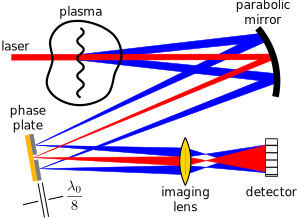
\includegraphics[width = 0.75 \textwidth]{%
    Chapters/InterferometricMethods/figs/pci_schematic.pdf}
  \caption[Schematic overview of a typical PCI system]{%
    Schematic overview of a typical PCI system.
    A plasma-density fluctuation weakly scatters an incident probe beam, and
    an off-axis parabolic mirror focuses the scattered and unscattered beams.
    An optical element known as a phase plate
    is placed at the focal plane of the parabolic mirror.
    The phase plate has a narrow groove of depth $\lambda_0 / 8$
    that imparts phase delay $\pi / 2$ to the unscattered beam,
    effectively converting the unscattered beam
    into an ``internal'' reference beam
    against which the scattered beams can be interfered.
    A lens, whose object plane sits at the plasma midplane,
    is then used to image the resulting radiation onto a detector array.}
  \label{fig:InterferometricMethods:pci_schematic}
\end{figure}


\subsection{Reference-beam generation with a phase plate}
PCI uses an optical element known as a \emph{phase plate}
to delay the unscattered beam by $\pi / 2$
relative to the scattered beams.
The phase plate is typically a reflective optical element
with a groove that is precisely fabricated
to have a depth of $\lambda_0 / 8$;
the unscattered beam reflects off of this groove, and
the corresponding $\lambda_0 / 4$-increase in path length
phase delays the unscattered beam by $\pi / 2$
relative to the scattered beams,
which reflect off of the non-grooved portions
(i.e.\ the ``face'') of the phase plate.
To boost the relative size of the fluctuating signal,
the phase groove typically reflects only a fraction $\eta < 1$
of the incident unscattered beam power, while
the phase-plate face reflects all of the scattered beam power.
Thus, by the action of the phase plate,
$1 \rightarrow i \sqrt{\eta}$ in the imaged electric field
(\ref{eq:InterferometricMethods:imaged_total_field_monochromatic_fluctuation_weak_coupling})
such that
\begin{equation}
  E_{\text{PCI}}(\vect{r}_{\image}, t)
  =
  i E_G(\vect{r}_{\image}, t) e^{i \bar{\phi}}
  \left[%
    \sqrt{\eta} + \tilde{\phi}_0 \cos\nu
  \right],
  \label{eq:InterferometricMethods:pci_imaged_field}
\end{equation}
and the corresponding intensity,
averaged over an optical cycle and
to first order in $\tilde{\phi}_0$, is
\begin{equation}
  I_{\text{PCI}}(\vect{r}_{\image}, t)
  =
  I_G(\vect{r}_{\image})
  \left[%
    \eta
    +
    2 \sqrt{\eta} \tilde{\phi}_0 \cos\nu
  \right].
  \label{eq:InterferometricMethods:pci_intensity}
\end{equation}
Here, $E_G(\vect{r}_{\image})$ and $I_G(\vect{r}_{\image})$
are the field and intensity profiles
of the unscattered Gaussian beam on the detector
in the \emph{absence} of the phase plate,
with $I_G(\vect{r}_{\image})$ being explicitly defined in
(\ref{eq:InterferometricMethods:Gaussian_beam_intensity}).
Equation
(\ref{eq:InterferometricMethods:pci_intensity})
should be contrasted with
(\ref{eq:InterferometricMethods:imaged_field_intensity}),
which gives the image-plane intensity
in the absence of the phase plate.
Thus, the phase plate converts the unscattered probe beam
into an effective reference beam for the scattered beams.


\subsection{Focal-plane separation of scattered beams}
Implicit in the use of the phase plate
is that the scattered and unscattered beams
are well-separated in space
such that the phase groove only affects the unscattered beam.
The 1\ts{st}-order scattered beams are angularly separated
from the unscattered beam by $\theta = k / k_0$, and,
in the far field ($z \gg z_R$),
the center of the scattered beam will fall outside of
the unscattered beam's 1/e $E$ radius if
\begin{equation}
  |k| \geq \frac{2}{w_0}.
  \label{eq:InterferometricMethods:kmin_for_far_field_beam_separation}
\end{equation}
However, CO$_2$ laser beams used to probe tokamak plasmas often have
$z_R \gg \SI{10}{\meter}$, so
the beam's far field is not easily accessible in typical lab settings.
Fortunately, the far-field diffraction pattern
can be equivalently accessed in the focal plane
of a focusing optic~\cite[Ch.~8]{born_and_wolf}.

The focal-plane location, beam size, and beam separation
can be easily determined.
Let the Gaussian probe beam have
an in-vessel 1/e $E$ waist radius of $w_0$,
and place a focusing optic of focal length $f$
a distance $s$ downstream from the in-vessel beam waist.
Then, the waist of the focused beam
will be located a distance $s'$ downstream of the focusing optic
and will have 1/e $E$ radius $w_0'$ given as
\begin{align}
  s' &= f \left( 1 + \frac{s - f}{z_R} \right),
  \\
  w_0' &= \frac{w_0 |f|}{\left[ (s - f)^2 + z_R^2 \right]^{1/2}},
\end{align}
where $z_R$ is the in-vessel Rayleigh length~\cite{self83}.
When $|s - f| \ll z_R$, as is typical for PCI,
the expressions for $s'$ and $w_0'$ reduce to
\begin{align}
  s' &\approx f,
  \label{eq:InterferometricMethods:focal_plane_location_rayleigh}
  \\
  w_0' &\approx \frac{2 |f|}{k_0 w_0}.
  \label{eq:InterferometricMethods:focal_plane_waist_rayleigh}
\end{align}
The spatial separation $\Delta$
of the scattered and unscattered beams in the focal plane
is found by applying the appropriate $ABCD$ ray matrices
from Table~\ref{table:ImagingSystems:ABCD_matrices}
to a ray scattered in the plasma midplane by angle $\theta$, i.e.\
\begin{align}
  \begin{pmatrix}
    \Delta
    \\
    \theta_{pp}
  \end{pmatrix}
  &=
  \begin{pmatrix}
    1 & s'
    \\
    0 & 1
  \end{pmatrix}
  \begin{pmatrix}
    1      & 0
    \\
    -1 / f & 1
  \end{pmatrix}
  \begin{pmatrix}
    1 & s
    \\
    0 & 1
  \end{pmatrix}
  \begin{pmatrix}
    0
    \\
    \theta
  \end{pmatrix},
  \notag
\end{align}
which, upon substitution of
of the focal plane location from
(\ref{eq:InterferometricMethods:focal_plane_location_rayleigh}) and
the scattering angle $\theta = k / k_0$,
simplifies to
\begin{equation}
  \Delta
  \approx
  \frac{k f}{k_0}.
  \label{eq:InterferometricMethods:phase_plate_beam_separation}
\end{equation}


\subsection{Low-$k$ cutoff of phase plate}
Now, let the phase-plate groove have a width $d$, as is shown in
Figure~\ref{fig:InterferometricMethods:phase_plate_beam_separation}.
Finite PCI response requires that (most of) the scattered beams
fall outside of the phase groove (i.e.\ $|\Delta| \geq d / 2$).
Application of the phase-plate beam-separation formula
(\ref{eq:InterferometricMethods:phase_plate_beam_separation})
then shows that there will be finite PCI response
for $|k| \geq k_g$, where
\begin{equation}
  k_g \equiv \frac{k_0 d}{2 f}.
  \label{eq:InterferometricMethods:pci_kmin_engineering}
\end{equation}
Here, the subscript $g$ is in reference
to the \emph{groove} of the phase plate.
Further, to provide the strongest phase contrast,
the unscattered beam should fall wholly within the phase groove
(i.e.\ $2 w_0' \leq d$);
substituting (\ref{eq:InterferometricMethods:focal_plane_waist_rayleigh})
for $w_0'$ then yields a constraint on the phase groove width
\begin{equation}
  d \geq \frac{4 f}{k_0 w_0},
  \label{eq:InterferometricMethods:phase_groove_constraint}
\end{equation}
and inserting (\ref{eq:InterferometricMethods:phase_groove_constraint}) into
(\ref{eq:InterferometricMethods:pci_kmin_engineering}) yields
\begin{equation}
  k_g \geq \frac{2}{w_0}.
  \label{eq:InterferometricMethods:pci_kmin_physics}
\end{equation}
As finite response requires that $|k| \geq k_g$, it follows that
(\ref{eq:InterferometricMethods:pci_kmin_physics}) is equivalent to
(\ref{eq:InterferometricMethods:kmin_for_far_field_beam_separation}),
which was derived by considering the far-field separation
of the scattered and unscattered beams.
Thus, PCI's low-$k$ cutoff
is ultimately constrained by the in-vessel beam size $w_0$,
with diffraction being the constraining physical mechanism.

\begin{figure}
  \centering
  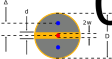
\includegraphics[width = 0.75 \textwidth]{%
    Chapters/InterferometricMethods/figs/phase_plate_beam_separation.pdf}
  \caption[Transverse phase-plate dimensions]{%
    Transverse phase-plate dimensions.
    The unscattered beam is shown in red, while
    the scattered beams are shown in blue.}
  \label{fig:InterferometricMethods:phase_plate_beam_separation}
\end{figure}


\subsection{High-$k$ cutoff of phase plate}
Let the phase plate have a diameter $D$, as is shown in
Figure~\ref{fig:InterferometricMethods:phase_plate_beam_separation}.
Detection of the scattered radiation
requires that (most of) the scattered beam reflect
from the face of the phase plate
(e.g.\ $\Delta \leq D / 2$).
Application of the phase-plate beam-separation formula
(\ref{eq:InterferometricMethods:phase_plate_beam_separation})
then shows that there will be finite PCI response for $|k| \leq k_D$ where
\begin{equation}
  k_D \equiv \frac{k_0 D}{2 f}.
  \label{eq:InterferometricMethods:pci_kmax_engineering}
\end{equation}


\subsection{Effect of phase plate on $m$\ts{th} scattered beam}
The effect of the PCI phase plate on the $m$\ts{th} scattered beam
is given by the complex-valued function $\mathcal{E}(\vect{r}_m, k)$,
which is derived and thoroughly discussed in
Appendix~\ref{app:PCIResponseIdentities}.
The relevant results are briefly summarized here for completeness.
Eq.~(\ref{eq:PCIResponseIdentities:transformation_Hermitian_decomposed})
shows that PCI's image-plane $\mathcal{E}(\vect{r}_m, k)$
readily reduces to
\begin{equation}
  \begin{aligned}
    \mathcal{E}(\vect{r}_{m,\image}, k_{\image})
    &=
    e^{-[x_{m,\image} / w(z_{m,\image})]^2}
    e^{i m k_{\image} x_{\image}}
    \\
    &\quad\times
    \left[%
      F(\vect{r}_{m,\image}, k_{\image})
      +
      G(\vect{r}_{m,\image}, k_{\image})
    \right],
  \end{aligned}
  \label{eq:InterferometricMethods:PCI_transformation_Hermitian_decomposed}
\end{equation}
where the phase-plate face acts on the $m$\ts{th} scattered beam via $F$, and
the phase-plate groove acts on the $m$\ts{th} scattered beam via $G$.
$F$ and $G$ are themselves defined in
(\ref{eq:PCIResponseIdentities:transformation_face}) and
(\ref{eq:PCIResponseIdentities:transformation_groove}).
Of particular note, $F$ is Hermitian with respect to $m$
\begin{equation}
  F(\vect{r}_{-m,\image}, k_{\image})
  =
  F^*(\vect{r}_{m,\image}, k_{\image}),
  \label{eq:InterferometricMethods:mth_beam_interaction_with_face_hermitian}
\end{equation}
while $G$ is anti-Hermitian with respect to $m$
\begin{equation}
  G(\vect{r}_{-m,\image}, k_{\image})
  =
  -G^*(\vect{r}_{m,\image}, k_{\image}).
  \label{eq:InterferometricMethods:mth_beam_interaction_with_groove_antihermitian}
\end{equation}
These symmetries imply
that $F(\vect{r}_{0,\image}, k_{\image})$ is purely \emph{real} and
that $G(\vect{r}_{0,\image}, k_{\image})$ is purely \emph{imaginary}.


\subsection{The imaged field and its intensity}
\label{sec:InterferometricMethods:pci:imaged_field_and_intensity}
Introducing the notational shorthand
$F_m \equiv F(\vect{r}_{m,\image}, k_{\image})$ and
$G_m \equiv G(\vect{r}_{m,\image}, k_{\image})$,
the weak-coupling ($\tilde{\phi}_0 \ll 1$), image-plane electric field from
(\ref{eq:InterferometricMethods:imaged_total_field_weak_coupling_Fourier_filtered})
readily reduces to
\begin{equation}
  \begin{aligned}
  E(\vect{r}_{\image}, t)
  \approx
  E_G(\vect{r}_{\image}, t)
  e^{i \bar{\phi}}
  \biggl\{%
    F_{0} + G_{0}
    &+
    i \frac{\tilde{\phi}_0}{2}
    \biggl[
      (F_{1} + G_{1}) e^{i \nu}
      \\
      &+
      (F_{-1} + G_{-1}) e^{-i \nu}
    \biggr]
  \biggr\},
  \end{aligned}
\end{equation}
where the approximation $w(z_m) \approx w(z)$ has been used,
$\nu$ is defined in (\ref{eq:InterferometricMethods:image_plane_nu}), and
$E_G(\vect{r}_{\image}, t)$ would be the image-plane electric field
of the unscattered beam in the \emph{absence} of the phase plate.
Now, recall that $F$ is Hermitian such that
$F_{-1} = F^{*}_{1}$ and $F_{0} = \real(F_{0})$ and
that $G$ is anti-Hermitian such that
$G_{-1} = -G^{*}_{1}$ and $G_{0} = {i \cdot \imag(G_{0})}$;
using these substitutions, the field further reduces to
\begin{equation}
  \begin{aligned}
    E(\vect{r}_{\image}, t)
    =
    E_G(\vect{r}_{\image}, t)
    e^{i \bar{\phi}}
    \biggl\{%
      &\real(F_0) - \tilde{\phi}_0 \imag(G_1 e^{i \nu})
      \\
      &+
      i \left[ \imag(G_0) + \tilde{\phi}_0 \real(F_1 e^{i \nu}) \right]
    \biggr\},
  \end{aligned}
\end{equation}
and the corresponding intensity,
averaged over an optical cycle and
to first order in $\tilde{\phi}_0$, is
\begin{equation}
  \begin{aligned}
    I_{\text{pci}}(\vect{r}_{\image}, t)
    &=
    I_G(\vect{r}_{\image})
    \biggl\{%
      |F_0|^2 + |G_0|^2
      \\
      &
      +
      2 \tilde{\phi}_0
      \bigl[%
        \imag(G_0) \real(F_1 e^{i \nu})
        -
        \real(F_0) \imag(G_1 e^{i \nu})
      \bigr]
    \biggr\},
  \end{aligned}
\end{equation}
where $I_G(\vect{r}_{\image})$
would be the intensity profile (averaged over an optical cycle)
of the unscattered beam in the \emph{absence} of the phase plate.
Using the fact that $e^{i \nu} = \cos\nu + {i \sin\nu}$,
$F_1 = \real(F_1) + {i \cdot \imag(F_1)}$, and
$G_1 = \real(G_1) + {i \cdot \imag(G_1)}$,
the image-plane intensity further reduces to
\begin{equation}
  \begin{aligned}
    I_{\text{pci}}(\vect{r}_{\image}, t)
    &=
    I_G(\vect{r}_{\image})
    \biggl\{%
      |F_0|^2 + |G_0|^2
      \\
      &+
      2 \tilde{\phi}_0
      \left[ \imag(G_0)\real(F_1) - \real(F_0)\imag(G_1) \right] \cos\nu
      \\
      &-
      2 \tilde{\phi}_0
      \left[ \imag(G_0)\imag(F_1) + \real(F_0)\real(G_1) \right] \sin\nu
    \biggr\}.
  \end{aligned}
  \label{eq:InterferometricMethods:PCI_image_plane_intensity_linear_combination_of_sine_and_cosine}
\end{equation}

Note that the linear combination
$A_I \cos \nu - A_Q \sin \nu$ for real $A_I$, $A_Q$, and $\nu$
can be rewritten as
\begin{align}
  A_I \cos \nu - A_Q \sin \nu
  &=
  A \cos(\nu + \theta),
  \label{eq:InterferometricMethods:linear_combination_of_sine_and_cosine}
\end{align}
where
$A = (A_I^2 + A_Q^2)^{1/2}$,
$\theta = \atantwo(A_Q, A_I)$,
and $\atantwo(A_Q, A_I)$ is the arctangent function of two arguments, which
uses the signs of $A_Q$ and $A_I$ to correctly determine the quadrant
corresponding to a tangent of $A_Q / A_I$.
Note that the notation is mnemonic:
$A_I$ is the amplitude of the ``in-phase'' ($I$) component
(i.e.\ proportional to the image of the assumed
cosine phase fluctuation $\tilde{\phi}(x, t)$ from
(\ref{eq:InterferometricMethods:cosine_phase_fluctuation})), and
$A_Q$ is the amplitude of the corresponding ``quadrature'' ($Q$) component.

As was the case for external reference-beam interferometry,
it is useful to characterize PCI's performance
relative to the saturation limits of a given detector.
Because $\tilde{\phi}_0 \ll 1$,
the PCI optical intensity
(\ref{eq:InterferometricMethods:PCI_image_plane_intensity_linear_combination_of_sine_and_cosine})
satisfies
\begin{align}
  I_{\text{pci}}(\vect{r}_{\image}, t)
  &\lesssim
  I_G(0)
  \left( |F_0|^2 + |G_0|^2 \right),
  \notag
\end{align}
where $I_G(0) = I_G(\rho_{\image} = 0, z_{\image})$ is convenient shorthand
for the peak intensity of the unscattered Gaussian probe beam at the detector
in the \emph{absence} of the phase plate.
To obtain optimal performance, select $I_G(0)$ such that
\begin{equation}
  I_{\text{sat}}
  =
  I_G(0)
  \left( |F_0|^2 + |G_0|^2 \right),
  \notag
\end{equation}
where $I_{\text{sat}}$ is the detector's linear saturation intensity.
Then, taking inspiration from
(\ref{eq:InterferometricMethods:linear_combination_of_sine_and_cosine}),
the image-plane PCI intensity fluctuations from
(\ref{eq:InterferometricMethods:PCI_image_plane_intensity_linear_combination_of_sine_and_cosine})
can be rewritten as
\begin{equation}
  \frac{\tilde{I}_{\text{pci}}(\vect{r}_{\image}, t)}{I_{\text{sat}}}
  =
  \frac{I_G(\vect{r}_{\image})}{I_G(0)}
  \cdot
  A_{\text{pci}}(k_{\image}, x_{\image})
  \cdot
  \tilde{\phi}_0
  \cos\left[ \nu + \theta_{\text{pci}}(k_{\image}, x_{\image}) \right],
\end{equation}
where
\begin{align}
  A_{\text{pci}}(k_{\image}, x_{\image})
  &\equiv
  \frac{2 A(k_{\image}, x_{\image})}{|F_0|^2 + |G_0|^2},
  \label{eq:InterferometricMethods:PCI_amplitude_response}
  \\
  \theta_{\text{pci}}(k_{\image}, x_{\image})
  &\equiv
  \atantwo(A_Q, A_I),
\end{align}
and
\begin{align}
  A(k_{\image}, x_{\image})
  &\equiv
  (A_I^2 + A_Q^2)^{1/2},
  \\
  A_I(k_{\image}, x_{\image})
  &\equiv
  \imag(G_0)\real(F_1) - \real(F_0)\imag(G_1),
  \label{eq:InterferometricMethods:PCI_response_AI}
  \\
  A_Q(k_{\image}, x_{\image})
  &\equiv
  \imag(G_0)\imag(F_1) + \real(F_0)\real(G_1).
  \label{eq:InterferometricMethods:PCI_response_AQ}
\end{align}

Thus, the action of the phase plate results in both
an amplitude response $A_{\text{pci}}(k_{\image}, x_{\image})$ and
a phase response $\theta_{\text{pci}}(k_{\image}, x_{\image})$
in PCI's image-plane intensity.
The on-axis responses $A_{\text{pci}}(k_{\image}, x_{\image} = 0)$ and
$\theta_{\text{pci}}(k_{\image}, x_{\image} = 0) = 0$
are consistent with previous derivations at $x_{\image} = 0$,
such as \cite[Eq.~2.141]{coda_phd} and \cite[Eq.~20]{rost_low_k_pci}.
The present work, however, explicitly accounts for
the spatial variation in the amplitude and phase responses
across the face of the detector.
Note that PCI operates as a nonlinear system
if there are substantial spatial variations in either
$A_{\text{pci}}$ or $\theta_{\text{pci}}$.
The amplitude and phase responses
can be easily evaluated numerically, and
the results for typical system parameters are shown in
Figure~\ref{fig:InterferometricMethods:phase_plate_amplitude_and_phase_response}.
As is colloquially understood, the amplitude response $A_{\text{pci}}$
drops precipitously for $|k| \lesssim k_g$.
(Additionally, the spatial variation in the amplitude response is minimal).
However, perhaps less well known, is the fact that
the phase response $\theta_{\text{pci}}$ exhibits
dramatic spatial variation for $|k| \lesssim k_g$.
This spatial variation biases the PCI-measured wavenumber $k_{\text{meas}}$
away from the true wavenumber $k$,
as shown in Figure~\ref{fig:InterferometricMethods:pci_wavenumber_upshift}.
The physical explanation for this effect is relatively simple:
a Gaussian beam can be decomposed into a set of infinite plane waves
with a finite spread in transverse wavevectors
(see Section~\ref{sec:InterferometricMethods:Gaussian_beam_diffraction:Gaussian_beam_definition}),
and only the components of the scattered beam
with transverse lab-frame wavenumbers $|k| \geq k_g$
are reflected from the phase-plate face and
produce measurable interference on the PCI detector.

\begin{figure}
  \centering
  \includegraphics[width = \textwidth]{%
    Chapters/InterferometricMethods/figs/pci_amplitude_and_phase_response.pdf}
    \caption[PCI amplitude and phase responses in object-plane coordinates
    ]{%
    PCI amplitude response $A_{\text{pci}}(k, x)$ and
    phase response $\theta_{\text{pci}}(k, x)$
    in object-plane coordinates.
    Spatial coordinates $x$ and wavenumbers $k$ are normalized
    to the 1/e $E$ radius of the in-vessel probe beam, $w_0$.
    The system magnification is $M = 0.5$, a fairly typical value.
    The dashed horizontal lines indicate
    the low-$k$ cutoff of the PCI phase-plate groove, $k_g$;
    here, $k_g = 2 / w_0$,
    which is the minimum value allowed by diffraction,
    as discussed in
    (\ref{eq:InterferometricMethods:pci_kmin_physics}).
    The phase-plate high-$k$ cutoff, $k_D$,
    is taken to be infinite.
    The reflectivity of the phase groove is $\eta = 0.17$,
    which is characteristic of the ZnSe typically
    employed in $\SI{10.6}{\micro\meter}$ optics.
    Note that the low-$k$ phase response $\theta_{\text{pci}}$
    exhibits dramatic spatial variation,
    which results in nonlinear PCI operation for $|k| \lesssim k_g$.
  }
\label{fig:InterferometricMethods:phase_plate_amplitude_and_phase_response}
\end{figure}

\begin{figure}
  \centering
  \includegraphics[width = \textwidth]{%
    Chapters/InterferometricMethods/figs/pci_wavenumber_upshift.pdf}
    \caption[Nonlinear upshift in low-$k$, PCI-measured wavenumber]{%
    PCI-measured wavenumber $k_{\text{meas}}$ vs.\ true wavenumber $k$.
    Wavenumbers are normalized
    to the 1/e $E$ radius of the in-vessel probe beam, $w_0$.
    The system magnification is $M = 0.5$, a fairly typical value.
    The dashed vertical lines indicate
    the low-$k$ cutoff of the PCI phase-plate groove, $k_g$;
    here, $k_g = 2 / w_0$,
    which is the minimum value allowed by diffraction,
    as discussed in
    (\ref{eq:InterferometricMethods:pci_kmin_physics}).
    For $|k| \gtrsim k_g$,
    $k_{\text{meas}}$ has a $1:1$ linear relationship with $k$;
    however, for $|k| \lesssim k_g$,
    $k_{\text{meas}}$ is \emph{not} linearly related to $k$.
    Thus, a transfer-function description of the PCI operation
    is only appropriate for wavenumbers above the low-$k$ cutoff
    ($|k| \gtrsim k_g$).
  }
\label{fig:InterferometricMethods:pci_wavenumber_upshift}
\end{figure}

Thus, for $|k| \lesssim k_g$, PCI operates as a nonlinear system
that cannot be described via a transfer function.
Practically speaking, PCI's nonlinear low-$k$ operation
prevents it from measuring the wavenumbers of low-$k$ fluctuations,
such as MHD and some ion-scale instabilities.
(Of course, because the PCI amplitude response $A_{\text{pci}}$
drops precipitously for $|k| \lesssim k_g$,
such low-$k$ fluctuations may be altogether invisible to PCI anyways).
For $|k| \gtrsim k_g$, however, a transfer function can be defined.
Specifically, for $|k| \gtrsim k_g$,
the phase-plate face reflects the scattered beam
($F_1 \rightarrow 1$), while
the phase-plate groove minimally affects the scattered beam
($G_1 \rightarrow 0$).
Further, assuming the majority of the unscattered beam
falls within the phase groove
(i.e.\ constraint (\ref{eq:InterferometricMethods:phase_groove_constraint})),
the phase-plate groove attenuates and phase shifts the unscattered beam
($G_0 \rightarrow i \sqrt{\eta}$), while
the phase-plate face minimally affects the unscattered beam
($F_0 \rightarrow 0$).
Thus, $\theta_{\text{pci}} \rightarrow 0$ and
$A_{\text{pci}} \rightarrow 2 / \sqrt{\eta}$ such that
the PCI transfer function can be defined as
\begin{equation}
  T_{\text{pci}}(k)
  =
  \begin{cases}
    \dfrac{2}{\sqrt{\eta}}, & |k| \gtrsim k_g \\
    \text{undefined},      & \text{otherwise}
  \end{cases}.
  \label{eq:InterferometricMethods:PCI_wavenumber_transfer_function}
\end{equation}
As presented here, for $|k| \gtrsim k_g$,
$T_{\text{pci}}$ is independent of the fluctuation wavenumber;
however, the finite sampling-volume effects
that accompany any real-world measurement
introduce a wavenumber dependence,
as discussed in
Section~\ref{sec:DesignConsiderations:geometric:finite_sampling_volume}.

As is the case with the homodyne interferometer,
the PCI technique does \emph{not} make an absolute measurement
of the phase-fluctuation amplitude $\tilde{\phi}_0$.
To see this, note that the PCI amplitude response $A_{\text{pci}}$
depends very sensitively on the system alignment,
with slight excursions of the unscattered beam
from the partially reflective phase-plate groove
onto the fully reflective phase-plate face
resulting in macroscopic changes to the power reaching the detector.
Further, power fluctuations at the beam source
can alter $I_G(\vect{r}_{\image})$.
Thus, there are three potentially dynamic quantities:
$\{\tilde{\phi}_0, I_G(\vect{r}_{\image}), A_{\text{pci}}\}$,
but there are only two potentially measurable quantities:
the equilibrium and fluctuating powers.
PCI systems on large, vibration-prone fusion devices
typically employ feedback stabilization
(see e.g.~\cite[Ch.~3.5]{coda_phd})
in order to dynamically maintain
the unscattered beam's alignment
on the phase-plate groove,
minimizing vibrational contamination of the PCI signal.
It is then possible, after measuring a calibration constant,
to \emph{estimate} the phase-fluctuation amplitude $\tilde{\phi}_0$ with PCI.


\section{Selecting an interferometric technique}
\label{sec:InterferometricMethods:selection}
Sections~\ref{sec:InterferometricMethods:interferometry}
and~\ref{sec:InterferometricMethods:pci}
detail external reference-beam interferometry and
phase contrast imaging (PCI), respectively.
The intent of this section is to synthesize these results and
to discuss the strengths and limitations
of these interferometric techniques
so that a suitable method can be selected for a given application.


\subsection{Sensitivity}
\label{sec:InterferometricMethods:selection:sensitivity}
The transfer functions in
Sections~\ref{sec:InterferometricMethods:interferometry}
and~\ref{sec:InterferometricMethods:pci}
specify the fraction of a given detector's dynamic range
that is occupied by the fluctuating signal.
If identical detectors are used for each interferometric method,
then an ``apples-to-apples'' comparison of fluctuation sensitivities
can be made by examining the amplitudes
of the corresponding transfer functions.
(See Section~\ref{sec:InterferometricMethods:selection:temporal_bandwidth}
for practical considerations regarding detector selection).
Just such a comparison is shown in
Figure~\ref{fig:InterferometricMethods:interferometric_method_transfer_functions}.
Clearly, for a given fluctuation ($|k| \gtrsim k_g$) and a given detector,
PCI has the best sensitivity.
Specifically, PCI is
$T_{\text{pci}} / T_{\text{hom}} = 2 / \sqrt{\eta}$
more sensitive than a comparable homodyne interferometer
($\phi_R - \bar{\phi} = \pi / 2$) and
$T_{\text{pci}} / T_{\text{het}} = 2 \pi \sqrt{2 / \eta}$
more sensitive than a comparable heterodyne interferometer.
Relative to homodyne interferometry,
PCI's enhanced sensitivity is wholly attributable
to the partial reflectivity ($\eta < 1$) of the phase-plate groove:
the decreased power in the unscattered beam
increases the fraction of the detector's dynamic range
occupied by the fluctuating signal.
The sensitivity deficit of heterodyne interferometry
relative to homodyne interferometry
has two physical origins:
first, the heterodyne interferometer
must capture the full sinusoidal waveform
of the heterodyne interference signal,
which mandates reduction of the mean optical intensity
(and, correspondingly, the fluctuating optical intensity)
at the detector by a factor of two
relative to that of the homodyne interferometer;
second, demodulation of the heterodyne interference signal
additionally attenuates the fluctuating signal.

\begin{figure}
  \centering
  \includegraphics[width = \textwidth]{%
    Chapters/InterferometricMethods/figs/interferometric_method_comparison.pdf}
  \caption[Comparison of interferometric-method transfer functions]{%
    A comparison of the transfer functions for
    PCI
    (\ref{eq:InterferometricMethods:PCI_wavenumber_transfer_function}),
    heterodyne interferometry
    (\ref{eq:InterferometricMethods:heterodyne_interferometer_wavenumber_transfer_function}),
    and homodyne interferometry
    (\ref{eq:InterferometricMethods:homodyne_interferometer_wavenumber_transfer_function},
    in the optimal fluctuation configuration
    with $\phi_R - \bar{\phi} = \pi / 2$).
    Object-plane wavenumbers $k$ are normalized
    to the 1/e $E$ radius of the in-vessel probe beam, $w_0$.
    The magnification of each system is taken to be $|M| = 0.5$,
    which is a representative ``typical'' value.
    The vertical, dashed lines indicate
    the low-$k$ cutoff of the PCI phase-plate groove, $k_g$;
    here, $k_g = 2 / w_0$,
    which is the minimum value allowed by diffraction,
    as discussed in
    (\ref{eq:InterferometricMethods:pci_kmin_physics}).
    The phase-plate high-$k$ cutoff, $k_D$,
    is taken to be infinite.
    The reflectivity of the PCI phase groove is $\eta = 0.17$,
    which is characteristic of the ZnSe typically
    employed in $\SI{10.6}{\micro\meter}$ optics.
    Because the PCI transfer function is not defined for $|k| \lesssim k_g$,
    the low-$k$ PCI amplitude response
    (\ref{eq:InterferometricMethods:PCI_amplitude_response})
    is indicated by the dash-dot curves instead.
  }
\label{fig:InterferometricMethods:interferometric_method_transfer_functions}
\end{figure}

The enhanced sensitivity of PCI and homodyne interferometry
relative to that of heterodyne interferometry
comes with several costs, however.
First, as previously discussed,
neither PCI nor homodyne interferometry
measure the absolute scale of phase fluctuations, while
heterodyne interferometry does.
Second, PCI depends sensitively on the position
of the unscattered beam relative to the phase-plate groove, and
homodyne interferometry depends sensitively on $\phi_R - \bar{\phi}$;
often, feedback stabilization is required
to dynamically maintain the optimal configuration
\cite[Ch.~3.5]{coda_phd}\cite{nazikian_rsi87}.
While feedback stabilization is an added technical complication,
it should be noted that such feedback
is expected to become more commonplace
for laser diagnostics on large fusion devices,
such as ITER's heterodyne interferometer
\cite{vanzeeland_TIP_rsi13}.
Finally, PCI cannot measure the equilibrium phase $\bar{\phi}$.
This makes intuitive sense:
$\bar{\phi}$ uniformly affects both the scattered and unscattered beams,
the PCI phase delays the unscattered beam
to generate an ``internal'' reference beam, and
the $\bar{\phi}$ information cancels in the resulting interference.
A homodyne interferometer operated with $\phi_R - \bar{\phi} = \pi / 2$
is similarly unable to measure $\bar{\phi}$.
In contrast, a heterodyne interferometer
can always measure both the equilibrium phase $\bar{\phi}$ and
the fluctuating phase $\tilde{\phi}$.


\subsection{Spatial bandwidth}
PCI's sensitivity comes at the additional expense of spatial bandwidth.
Specifically, the creation of an ``internal'' reference beam
via spatial filtering
produces a low-$k$ cutoff in the PCI response, as shown in
Figure~\ref{fig:InterferometricMethods:interferometric_method_transfer_functions}.
The minimum size of this cutoff is
set by diffraction of the in-vessel probe beam
(\ref{eq:InterferometricMethods:pci_kmin_physics}), but
it is not uncommon for the realized cutoff
(\ref{eq:InterferometricMethods:pci_kmin_engineering})
to be $\sim 2-3\times$ larger than the diffraction limit.
As shown in Figures~\ref{fig:InterferometricMethods:phase_plate_amplitude_and_phase_response}
and \ref{fig:InterferometricMethods:pci_wavenumber_upshift},
PCI operates as a nonlinear system below its low-$k$ cutoff,
preventing a transfer-function description of its low-$k$ behavior.
In contrast, by using an external reference beam,
homodyne and heterodyne interferometers
operate as linear systems over the entire wavenumber spectrum and
are even capable of making measurements at $k = 0$.

Now, colloquially, interferometry is considered a ``low-$k$'' technique, and
PCI is considered a ``high-$k$'' technique.
However, as detailed in
Section~\ref{sec:InterferometricMethods:Gaussian_beam_diffraction:from_plasma_density_fluctuations},
for a given probe beam and a given fluctuation $\tilde{\phi}$,
the laser-plasma interaction is \emph{identical}
for both interferometry and PCI.
Further, the high-$k$ optical capabilities of interferometry and PCI
are governed by the size of the collection optics
and finite sampling-volume effects~\cite{bravenec_rsi95}.
Thus, there is nothing that intrinsically limits
interferometry to low-$k$ measurements ---
an interferometer's high-$k$ limit
can be just as high, if not higher,
than that of a given PCI system.
However, as discussed in
Section~\ref{sec:InterferometricMethods:selection:sensitivity},
PCI is \emph{more sensitive} to fluctuations
than a comparable interferometer, and,
assuming a Kolmogorov-like fluctuation spectrum
$S(k) \propto k^{-p}$ for some positive $p$,
PCI's superior sensitivity may allow it
to detect high-$k$ fluctuations
that are too weak to be seen by an interferometer.


\subsection{Temporal bandwidth}
\label{sec:InterferometricMethods:selection:temporal_bandwidth}
Detector bandwidth is often the dominant constraint
of an interferometric system's temporal bandwidth.
Homodyne interferometry and PCI require
\begin{equation}
  \omega_{\text{det}} > \omega,
  \qquad \qquad \quad% \qquad
  \text{homodyne interferometry, PCI,}
\end{equation}
where
$\omega_{\text{det}}$ is the angular cutoff frequency of the detector and
$\omega$ is the angular frequency of the fluctuation.
Heterodyne interferometry, however, requires
\begin{equation}
  \omega_{\text{det}} > \Delta \omega_0 + \omega,
  \qquad
  \text{heterodyne interferometry,}
\end{equation}
where $\Delta \omega_0$ is the (angular) intermediate frequency.
Further, proper reconstruction of the baseband signal
from the heterodyne interference signal requires $\omega < \Delta \omega_0$.

Thus, for a given fluctuation $\omega \ll \Delta \omega_0$,
heterodyne interferometry requires a much faster detector
than homodyne interferometry or PCI\@.
For the HgCdTe detectors typically used at $\SI{10.6}{\micro\meter}$,
cooling the active element of the detector
reduces detector noise and increases the detector response
at the expense of reduced $\omega_{\text{det}}$.
Thus, for low--bandwidth applications ($\omega \ll \Delta \omega_0$),
homodyne interferometry and PCI may be able to use
slower, cooled detectors that are less noisy than
the comparable faster, warmer detectors
required for heterodyne interferometry.
The use of less noisy detectors
may produce sensitivity gains for PCI and homodyne interferometry
relative to heterodyne interferometry.
Although use of a ``slow'' detector prevents measurements
of broadband fluctuations beyond the detector cutoff,
it \emph{is} possible to measure coherent, high-frequency fluctuations
well beyond the detector cutoff ($\omega \gg \omega_{\text{det}}$)
by rapidly modulating the intensity of the probe beam
\cite[Sec.~3.3.1]{tsujii_phd}.


\bibliographystyle{plainurl}
\bibliography{references}
%
\chapter{Design considerations for a heterodyne interferometer}
\label{ch:DesignConsiderations}
While Chapter~\ref{ch:InterferometricMethods} discusses the
\emph{optical} foundations for various interferometric methods,
most real-world optical diagnostics are complex, integrated systems
requiring precise interplay between various components, such as
lasers, optics, detectors, and electronics.
Optimizing the performance of a given diagnostic
requires careful consideration
of each component and its role in the measurement.
Some of these considerations are generic, and
some of them are diagnostic specific.

This chapter examines numerous design considerations
that are relevant to heterodyne interferometry.
The sections are arranged in roughly sequential order,
beginning with the interference signal at the detector and
proceeding through successive downstream components
until reaching the system's digitizer.
In particular, Section~\ref{sec:DesignConsiderations:geometric}
discusses the geometric effects that
set the interferometer's wavenumber response and
the magnitude of the interferometer's heterodyne signal.
Section~\ref{sec:DesignConsiderations:intensity}
explores heterodyne measurements made
beyond the saturation-intensity limit of a given detector.
Sections~\ref{sec:DesignConsiderations:phase_noise} and
\ref{sec:DesignConsiderations:amplitude_noise}
reveal how phase noise and amplitude noise, respectively,
can creep into the interferometer's measurements.
Section~\ref{sec:DesignConsiderations:demodulation}
describes demodulation of the heterodyne interference signal and
the distortion of the baseband phase signal
that results from demodulator imperfections.
Finally, Section~\ref{sec:DesignConsiderations:quantization}
discusses the signal quantization
that necessarily results
from generating a digital record.
The below design considerations will be referenced extensively in
Chapter~\ref{ch:Implementation}, which
describes the addition of a heterodyne interferometer
to the pre-existing phase contrast imaging (PCI) diagnostic
on the \diiid\space tokamak.


\section{Geometric considerations}
\label{sec:DesignConsiderations:geometric}
Several geometric effects substantially influence
the performance of a heterodyne interferometer.
Section~\ref{sec:DesignConsiderations:geometric:finite_sampling_volume}
reveals how the imaging system's magnification $M$ and
the detector's size and shape
determine the interferometer's wavenumber response.
Section~\ref{sec:DesignConsiderations:geometric:beam_mismatch}
discusses the implications of mismatches between
the plasma beam's and the reference beam's spatial structures and
develops a criterion for the required level of matching.


\subsection{Aperture diffraction}
Diffraction from finite-aperture optics was neglected in
Chapter~\ref{ch:InterferometricMethods}'s
transfer-function derivations.
For a propagating Gaussian beam,
this neglect of aperture diffraction is a reasonable approximation if
\begin{equation}
  a_{\text{eff}} \geq \frac{3}{2} w(z),
  \label{eq:DesignConsiderations:aperture_radius_for_minimal_diffraction}
\end{equation}
for each aperture, where
$a_{\text{eff}}$ is the effective aperture radius and
$w(z)$ is the beam's 1/e $E$ radius at the aperture location
\cite{campbell_josa69, rost_diffraction_pc14}.
For a circular aperture of radius $a$,
the effective aperture radius is simply $a_{\text{eff}} = a$
for a beam propagating along the optical axis
(e.g.\ the unscattered beam from
Sec.~\ref{sec:InterferometricMethods:Gaussian_beam_diffraction:from_plasma_density_fluctuations});
however, for a beam located $\rho(z)$ away from the optical axis
(e.g.\ the upscattered or downscattered beam from
Sec.~\ref{sec:InterferometricMethods:Gaussian_beam_diffraction:from_plasma_density_fluctuations}),
the effective aperture radius is $a_{\text{eff}} = a - \rho(z)$.


\subsection{Beam coalignment}
For the moment, assume a plane-wave representation
for both the reference beam and the unscattered probe beam.
Specifically, let the spatial dependence
of the reference beam be given by
\begin{equation}
  \vect{E}_R(\vect{r})
  =
  E_0 \hat{\vect{x}}
  \cdot
  e^{i k_0 z},
\end{equation}
and let the unscattered probe beam
be misaligned with the reference beam
by angle $\theta \ll 1$ such that,
to lowest order in $\theta$,
the spatial dependence of the unscattered probe beam is
\begin{equation}
  \vect{E}_P(\vect{r})
  \approx
  E_0 \hat{\vect{x}}
  \cdot
  e^{i k_0 (z + \theta x)}.
\end{equation}
The total intensity (averaged over an optical cycle) is then
\begin{align}
  I
  =
  \frac{c \varepsilon_0}{2}
  \left|
    \vect{E}_R + \vect{E}_P
  \right|^2
  \approx
  2 I_0 \left[ 1 + \cos(k_0 \theta x) \right],
\end{align}
where $I_0 = c \varepsilon_0 E_0^2 / 2$
is the corresponding intensity of a single beam.
Here, the $\cos(k_0 \theta x)$ term
corresponds to the interference between the two beams, and
the unity term corresponds to the intensity of each individual beam.
Optimizing the interference signal requires
alignment of the beam polarizations and
minimization of the misalignment angle $\theta$.
If the interference is measured by a detector
with an extent $s_x$ in the $x$-direction,
the misalignment-induced phase $k_0 \theta x$
should change by much less than $2 \pi$ across the detector face;
i.e.\ $|k_0 \theta s_x| \ll 2 \pi$ or
\begin{equation}
  |\theta|
  \ll
  \frac{\lambda_0}{s_x}
  \approx
  0.6^{\circ},
  \label{eq:DesignConsiderations:coalignment_constraint}
\end{equation}
where $\lambda_0 = 2 \pi / k_0$ is the beam wavelength, and
$\lambda_0 = \SI{10.6}{\micro\meter}$ and
$s_x = \SI{1}{\milli\meter}$
have been used for the evaluation.
Coalignment constraint (\ref{eq:DesignConsiderations:coalignment_constraint})
has design implications for CO$_2$ interferometers
operated at magnetic fusion experiments, which
are often characterized by large, pulsed electromagnets
whose operation may contort the machine and produce vibrations,
potentially destroying the beam coalignment.


\subsection{Mismatch between beam spatial structures}
\label{sec:DesignConsiderations:geometric:beam_mismatch}
The external reference-beam interferometry derivations
in Section~\ref{sec:InterferometricMethods:interferometry}
assumed that the reference beam was exactly matched
in both amplitude and spatial structure
to the unscattered probe beam.
This is obviously an idealization
that, at best, can only be approximately met in experiment.
This section discusses the geometric effects
of such imperfections in beam matching.

The derivation of the heterodyne intensity
(\ref{eq:InterferometricMethods:heterodyne_intensity})
can be easily generalized to account for
the geometric effects of unmatched reference and probe beams.
Namely, let the image-plane probe radiation be given by
\begin{equation}
  E_P(\vect{r}_{\image}, t)
  \approx
  E_{G,P}(\vect{r}_{\image}, t)
  e^{i \bar{\phi}}
  \left[%
    1
    +
    i \tilde{\phi}_0 \cos\nu
  \right],
\end{equation}
and let the corresponding reference beam be given by
\begin{equation}
  E_R(\vect{r}_{R}, t)
  =
  E_{G,R}(\vect{r}_{R}, t) e^{-i \Delta\omega_0 t},
\end{equation}
where $\vect{r}_{\image} = (x_{\image}, y_{\image}, z_{\image})$,
\begin{equation}
  \vect{r}_{R}
  =
  \vect{r}_{\image}
  +
  (0, 0, z_{R} - z_{\image}),
\end{equation}
and $E_{G,j}$ is a Gaussian beam
with angular frequency $\omega_0$,
waist amplitude $E_{0,j}$, and
waist 1/e $E$ radius $w_{0,j}$.
If $z_R \neq z_{\image}$,
the reference beam's waist sits at a different location
than that of the unscattered probe beam.
Under these circumstances, the heterodyne intensity becomes
\begin{equation}
  \begin{aligned}
    I_{\text{het}}(\vect{r}_{\image}, z_R, t)
    =
    2 I_{G,P}(\vect{r}_{\image})
    \bigl[%
      &\alpha_{\text{DC}}
      +
      \alpha_{\text{AC}}
      \cos(\Delta \omega_0 t + \bar{\phi}_{\text{eff}})
      \\
      &-
      \tilde{\phi}_0 \alpha_{\text{AC}}
      \sin(\Delta \omega_0 t + \bar{\phi}_{\text{eff}}) \cos\nu
    \bigr],
  \end{aligned}
  \label{eq:DesignConsiderations:heterodyne_intensity}
\end{equation}
where
\begin{equation}
  \bar{\phi}_{\text{eff}}
  =
  \bar{\phi}
  +
  \bigl[ \phi_{G,P}(\vect{r}_{\image}) - \phi_{G,R}(\vect{r}_R) \bigr]
\end{equation}
is the effective bulk phase,
\begin{equation}
  \phi_{G,j}(\vect{r})
  =
  k_0 z + \frac{k_0 \rho^2}{2 R_j(z)} - \psi_j(z)
\end{equation}
is the phase of Gaussian beam $j \in \{P, R\}$
(i.e.\ $E_{G,j}(\vect{r}) = |E_{G,j}(\vect{r})| e^{i \phi_{G,j}(\vect{r})}$),
\begin{align}
  \alpha_{\text{DC}}
  &=
  \frac{1}{2}\left[%
    1
    +
    \frac{I_{G,R}(\vect{r}_R)}{I_{G,P}(\vect{r}_{\image})}
  \right],
  \\
  \alpha_{\text{AC}}
  &=
  \sqrt{\frac{I_{G,R}(\vect{r}_R)}{I_{G,P}(\vect{r}_{\image})}},
\end{align}
are geometric factors that describe the amplitudes
of the DC and AC components of the heterodyne signal, and
\begin{equation}
  I_{G,j}(\vect{r})
  =
  \frac{c \varepsilon_0 |E_{G,j}(\vect{r})|^2}{2}
\end{equation}
is the intensity profile (averaged over an optical cycle)
of Gaussian beam $j \in \{P, R\}$.
Note that (\ref{eq:DesignConsiderations:heterodyne_intensity}) readily reduces to
(\ref{eq:InterferometricMethods:heterodyne_intensity})
if $E_{G,R}(\vect{r}_R) = E_{G,P}(\vect{r}_{\image})$.

It is worth discussing the implications of heterodyne intensity
(\ref{eq:DesignConsiderations:heterodyne_intensity}).
First, the AC component of the intensity
carries the desired phase information, and
maximizing the ratio of the AC signal to the DC signal requires that
$I_{G,R}(\vect{r}_R) = I_{G,P}(\vect{r}_{\image})$.
Second, note that the effective bulk phase $\bar{\phi}_{\text{eff}}$
is dependent on the geometry of the reference beam and
the unscattered probe beam.
Specifically, in the context of measuring
the plasma-induced bulk phase $\bar{\phi}$,
note that
\begin{equation}
  \bar{\phi}_{\text{eff}}(\rho_{\image}=0)
  =
  \bar{\phi}
  +
  k_0 (z_{\image} - z_R)
  -
  \left[ \psi_P(z_{\image}) - \psi_R(z_R) \right].
\end{equation}
If $z_{\image}$ and $z_R$ are fixed,
then the beam-geometry contributions to
$\bar{\phi}_{\text{eff}}(\rho_{\image} = 0)$
constitute an unimportant DC offset that can be removed
via baseline subtraction;
however, experiments are typically plagued by vibrations, and
even small changes to $z_{\image}$ and $z_R$
can make significant time-dependent contributions to
$\bar{\phi}_{\text{eff}}(\rho_{\image} = 0)$ at CO$_2$ probe wavelengths.
As such, deconvolving the plasma-induced and vibration-induced contributions
to $\bar{\phi}_{\text{eff}}(\rho_{\image} = 0)$
requires interferometric measurements
at two distinct wavelengths (i.e.\ two-color interferometry)
\cite{carlstrom_rsi88}.
However, such vibrations occur on slow time-scales
(e.g.\ $f_{\text{vib}} \lesssim \SI{5}{\kilo \hertz}$),
and phase measurements at a \emph{single} wavelength are sufficient
to quantify plasma-induced phase fluctuations
at frequencies above $f_{\text{vib}}$
\cite{vanzeeland_ppcf05}.
Note that the beam geometry also imparts
a spatially dependent, curvature-induced phase shift
\begin{align}
  \delta\phi_{\kappa}(\rho_{\image})
  &=
  \bar{\phi}_{\text{eff}}(\rho_{\image})
  -
  \bar{\phi}_{\text{eff}}(\rho_{\image} = 0)
  \notag \\
  &=
  \frac{k_0 \rho_{\image}^2}{2}
  \left[\frac{1}{R_P(z_{\image})} - \frac{1}{R_R(z_R)} \right],
\end{align}
which can result in signal loss and distortion of the measured wavenumber.
To see this, assume that the radiation is interfered on a detector array,
as shown in Fig.~\ref{fig:DesignConsiderations:detector_array}.
As a detector element produces a signal
proportional to the average intensity across its face,
there will be substantial signal loss
if there are large curvature-induced phase shifts
across the element's face
(i.e.\ $\delta\phi_{\kappa}(s_x / 2) \gtrsim \pi$ or
$\delta\phi_{\kappa}(s_y / 2) \gtrsim \pi$).
Further, if there are large curvature-induced phase shifts
across the length of the detector array,
the spatial structure of the intensity
will \emph{not} correspond to the spatial structure
of the plasma fluctuation.
The latter is the more conservative constraint
on the curvature-induced phase shift.
Assuming that the detector array shown in
Fig.~\ref{fig:DesignConsiderations:detector_array}
consists of $N_{\text{el}}$ detector elements and
that the inter-element spacing is negligible ($\delta_x \ll s_x$),
the criterion for negligible curvature-induced phase shifts
$\delta\phi_{\kappa, \text{max}}
=
\delta\phi_{\kappa}(\rho_{\image, \text{max}})
\ll
\pi$
becomes
\begin{equation}
  \frac{k_0}{8}
  \left[ (N_{\text{el}} s_x)^2 + s_y^2 \right]
  \left| \frac{1}{R_P(z_{\image})} - \frac{1}{R_R(z_R)}\right|
  \ll
  \pi.
\end{equation}

\begin{figure}
  \centering
  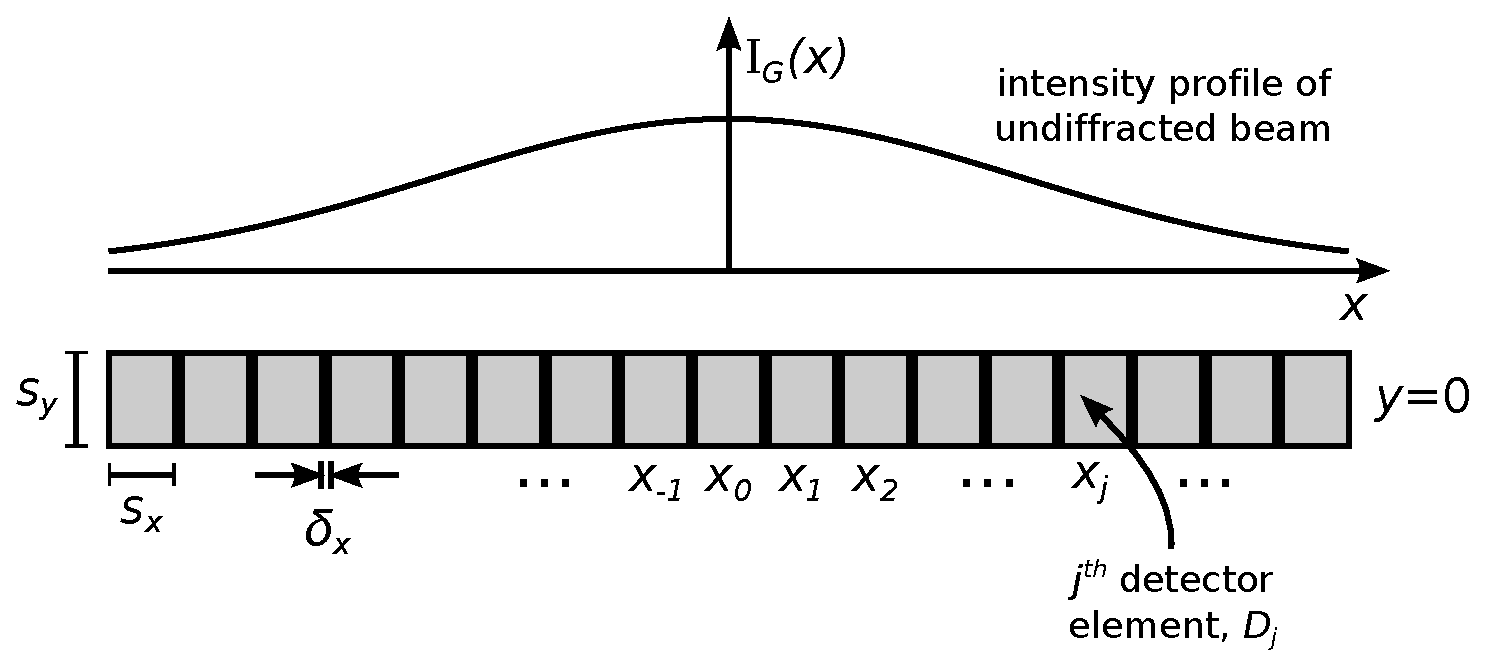
\includegraphics[width = \textwidth]{%
    Chapters/DesignConsiderations/figs/detector_array.pdf}
  \caption[Finite sampling volumes in a detector array]{%
    The probe radiation and the reference beam
    are interfered on a detector array.
    The array consists of numerous detector elements,
    each of size $s_x \times s_y$ and with interelement spacing $\delta_x$.
    The unscattered beam is centered on $x = x_0$ and $y = 0$, and
    its intensity profile varies only weakly over any given element.
    The finite size of each detector element tends to attenuate
    short wavelength components of the incident optical signal.
  }
\label{fig:DesignConsiderations:detector_array}
\end{figure}


\subsection{Finite sampling-volume effects}
\label{sec:DesignConsiderations:geometric:finite_sampling_volume}
Practically speaking, detection is always effected
via detector elements of \emph{finite} size,
with the output of each detector element
corresponding to the incident intensity
\emph{averaged} over the element's active area.
This averaging acts as a low-pass filter in the spatial domain and
is referred to as the finite sampling-volume effect~\cite{bravenec_rsi95}.

Finite sampling-volume effects dictate
a heterodyne interferometer's wavenumber response~\cite{davis_rsi16}.
To see this, assume that measurements
are made with the detector array shown in
Fig.~\ref{fig:DesignConsiderations:detector_array}.
Let the $j$\ts{th} detector element $D_j$ be centered on $x_{\image,j}$
and $y_{\image} = 0$.
Integrating the optical intensity $\tilde{I}_{IQ}(\vect{r}_{\image}, t)$
corresponding to fluctuations in the baseband signal from
(\ref{eq:InterferometricMethods:heterodyne_total_fluctuating_intensity})
over the face of detector element $D_j$ yields
the corresponding optical power
\begin{align}
  \tilde{P}_{IQ,j}(t)
  &=
  \int_{D_j} \tilde{I}_{IQ}(\vect{r}_{\image}, t) dA
  \notag \\
  &\approx
  I_G(\vect{r}_{\image,j}) s_y
  \int_{x_{\image,j} - s_x / 2}^{x_{\image,j} + s_x / 2}
  \tilde{\phi}(x_{\image}, t)
  dx_{\image};
  \label{eq:DesignConsiderations:fluctuating_baseband_equivalent_optical_power_per_element_v1}
\end{align}
here, the intensity profile $I_G(\vect{r}_{\image})$
has been assumed to be approximately constant
over the face of the detector element.
Because (\ref{eq:DesignConsiderations:fluctuating_baseband_equivalent_optical_power_per_element_v1})
is linear in $\tilde{\phi}$,
it is suitable to consider a single Fourier mode
\begin{equation}
  \tilde{\phi}(x_{\image}, t)
  =
  \tilde{\phi}_0 \cos(k_{\image} x_{\image} - \omega t)
\end{equation}
for which (\ref{eq:DesignConsiderations:fluctuating_baseband_equivalent_optical_power_per_element_v1})
reduces to
\begin{equation}
  \tilde{P}_{IQ,j}(t)
  =
  I_G(\vect{r}_{\image,j}) A
  \cdot
  T_{\text{fsv}}(k_{\image})
  \cdot
  \tilde{\phi}_0 \cos(k_{\image} x_{\image} - \omega t),
  \label{eq:DesignConsiderations:fluctuating_baseband_equivalent_optical_power_per_element_v2}
\end{equation}
where $A = s_x s_y$ is the area of the detector element,
\begin{equation}
  T_{\text{fsv}}(k_{\image})
  \equiv
  \sinc\left( \frac{k_{\image}}{k_{\text{fsv},\image}} \right)
  \label{eq:DesignConsiderations:finite_sampling_volume_transfer_function}
\end{equation}
is the finite sampling-volume transfer function,
\begin{equation}
  \sinc(x) = \frac{\sin(\pi x)}{\pi x}
  \label{eq:DesignConsiderations:normalized_sinc}
\end{equation}
is the normalized sinc function, and
\begin{equation}
  k_{\text{fsv},\image} = \frac{2 \pi}{s_x}
  \label{eq:DesignConsiderations:finite_sampling_volume_cutoff_image_plane}
\end{equation}
is the first zero of $T_{\text{fsv}}(k_{\image})$.
Recalling that an object-plane wavenumber $k$
is imaged as $k_{\image} = k / M$
in a magnification-$M$ imaging system,
the corresponding object-plane finite sampling-volume wavenumber cutoff is
\begin{equation}
  k_{\text{fsv}} = \frac{2 \pi M}{s_x}.
  \label{eq:DesignConsiderations:finite_sampling_volume_cutoff}
\end{equation}
Now, as in Section~\ref{sec:InterferometricMethods:interferometry:heterodyne},
select the central intensity of the unscattered beam at the detector to be
$I_G(0) = I_{\text{sat}} / 4$, where
$I_{\text{sat}}$ is the detector's linear saturation intensity,
such that
\begin{equation}
  \frac{\tilde{P}_{IQ,j}(t)}{I_{\text{sat}} A}
  =
  \frac{I_G(\vect{r}_{\image,j})}{I_G(0)}
  \cdot
  T_{\text{het}}(k_{\image})
  \cdot
  \tilde{\phi}_0 \cos(k_{\image} x_{\image} - \omega t),
\end{equation}
where
\begin{equation}
  T_{\text{het}}(k_{\image})
  =
  \frac{1}{4} \cdot T_{\text{fsv}}(k_{\image})
  \label{eq:DesignConsiderations:heterodyne_interferometer_wavenumber_transfer_function}
\end{equation}
is the heterodyne interferometer's wavenumber transfer function.
In the limit $s_x \rightarrow 0$, $T_\text{fsv} \rightarrow 1$ and
the heterodyne interferometer's wavenumber transfer function reduces to
(\ref{eq:InterferometricMethods:heterodyne_interferometer_wavenumber_transfer_function}).
Thus, finite sampling-volume effects
introduce a wavenumber dependence into $T_{\text{het}}$,
as shown in Fig.~\ref{fig:DesignConsiderations:fsv_effects}.
Note that finite sampling-volume effects
introduce similar wavenumber dependencies
into the transfer functions of the homodyne interferometer and PCI.

\begin{figure}
  \centering
  \includegraphics[width = \textwidth]{%
    Chapters/DesignConsiderations/figs/fsv_effects.pdf}
  \caption[Transfer function of heterodyne interferometer with finite sampling-volume effects]{%
    The wavenumber transfer function for a heterodyne interferometer
    with finite sampling-volume (FSV) effects and without FSV effects.
  }
\label{fig:DesignConsiderations:fsv_effects}
\end{figure}


\section{Intensity considerations}
\label{sec:DesignConsiderations:intensity}
Ideally, a photovoltaic detector produces an output voltage
\begin{equation}
  V(t) = \mathcal{R}_0 \cdot I(t),
\end{equation}
where $\mathcal{R}_0$ is the detector responsivity and
$I(t)$ is the incident optical intensity.
However, every real-world detector has a saturation intensity $I_{\text{sat}}$
beyond which the output voltage ceases to be a linear function
of the incident optical intensity; that is,
the detector responsivity has an intensity dependence $\mathcal{R}(I)$, and
the detector voltage can be more generally written as
\begin{equation}
  V(t) = \mathcal{R}\left( I(t) \right) \cdot I(t).
\end{equation}
Here, $\mathcal{R}(I)$ is an arbitrary monotonically increasing function
of the incident optical intensity $I$.
Despite the potentially nonlinear response,
the detector voltage remains periodic in $2 \pi / \Delta \omega_0$ and
can be expanded in a Fourier series as
\begin{equation}
  V(t)
  =
  V_0
  +
  \sum_{n = 1}^{\infty}
  V_n \cos\left( n \Delta \omega_0 t + \theta_n \right),
\end{equation}
where $V_n$ and $\theta_n$ are the amplitude and phase, respectively,
of the $n\ts{th}$ harmonic.
Thus, a nonlinear detector response produces
higher-order harmonics in the signal.
In general, $V_n$ and $\theta_n$ can vary in time,
producing sidebands about each harmonic.
Provided the bandwidth of these fluctuations is sufficiently low,
there will be no spectral overlap
between the sidebands of adjacent harmonics, and
bandpass filtering the detector signal about $\Delta \omega_0$ yields
\begin{equation}
  V(t) \approx V_1 \cos[\Delta \omega_0 t + \theta_1(t)]
\end{equation}
with $\theta_1(t) = \phi(t)$, where
$\phi(t)$ is the optical phase shift
between the plasma and reference arms of the interferometer.
However, for fluctuations with sufficiently high bandwidth
(e.g.\ $\omega \sim \Delta\omega_0 / 2$),
the sidebands of adjacent harmonics begin to overlap,
potentially corrupting the phase measurement,
as demonstrated by the example in
Fig.~\ref{fig:DesignConsiderations:nonlinear_heterodyne_detection}.
When operating in the saturated regime,
the heterodyne interferometer transfer function
(\ref{eq:InterferometricMethods:heterodyne_interferometer_wavenumber_transfer_function})
should be multiplied by the prefactor $(V_1 / V_{\text{sat}})$, where
$V_1$ is the amplitude of the heterodyne frequency's fundamental harmonic and
$V_{\text{sat}}$ is the output voltage of the detector
when the incident optical intensity
is equal to the saturation intensity $I_{\text{sat}}$.

\begin{figure}
  \centering
  \includegraphics[width = \textwidth]{%
    Chapters/DesignConsiderations/figs/nonlinear_heterodyne_detection.pdf}
  \caption[Heterodyne detection beyond the saturation intensity]{%
    Heterodyne detection beyond the saturation intensity with
    $\Delta\omega_0 = 2\pi \cdot \SI{30}{\mega\hertz}$ and
    $\omega = 2 \pi \cdot \SI{16}{\mega\hertz}$.
    (Top panel): Various detector saturation models.
    The linear model exhibits no saturation,
    the hard saturation model limits the output voltage
    to $V_{\text{sat}}$ when the incident optical intensity
    exceeds $I_{\text{sat}}$, and
    the arctangent saturation model exhibits $\SI{1}{\deci\bel}$ compression
    when the incident optical intensity is $I_{\text{sat}}$.
    (2\ts{nd} panel): The intermediate frequency (IF) waveforms
    corresponding to each saturation model when
    $I_{\text{max}} = 10 \, I_{\text{sat}}$.
    The arctangent and hard saturation models distort the IF waveform,
    producing numerous higher-order harmonics.
    (3\ts{rd} panel): Autospectral densities of the IF waveforms.
    The IF waveforms all exhibit peaks at
    the $\SI{30}{\mega\hertz}$ fundamental and
    its corresponding sidebands at
    $\SI{30}{\mega\hertz} \pm \SI{16}{\mega\hertz}$.
    However, the saturated IF waveforms
    also exhibit peaks at the second harmonic ($\SI{60}{\mega\hertz}$)
    and its corresponding sidebands
    ($\SI{60}{\mega\hertz} \pm \SI{16}{\mega\hertz}$).
    (Bottom panel): Autospectral densities of the demodulated phase.
    Note that the $\SI{16}{\mega\hertz}$ fluctuation is correctly identified
    when demodulating all of the IF waveforms.
    However, the saturated IF waveforms also produce
    a \emph{spurious} $\SI{14}{\mega\hertz}$ fluctuation,
    which is attributable to the overlap of
    the $\SI{30}{\mega\hertz}$ and $\SI{60}{\mega\hertz}$ sidebands.
  }
\label{fig:DesignConsiderations:nonlinear_heterodyne_detection}
\end{figure}


\section{Phase noise: sources and effects}
\label{sec:DesignConsiderations:phase_noise}
All real-world oscillators exhibit phase noise.
The spectral properties of oscillator phase noise and
the implications for instruments that rely on oscillators
are discussed in
Appendix~\ref{app:OscillatorPhaseNoise}.


\subsection{Umatched optical path lengths}
The external reference-beam interferometry derivations
in Section~\ref{sec:InterferometricMethods:interferometry}
assumed that the laser's angular frequency was fixed
at its nominal value $\omega_0$.
However, the angular frequency of any \emph{real} laser
will exhibit small fluctuations in time,
much like any other real-world oscillator
\cite[Sec.~1.7]{siegman_lasers}.
The electric field of such a Gaussian beam
is well-described by
\begin{equation}
  E_G(\vect{r}, t)
  =
  E_G(\vect{r})
  e^{-i [\omega_0 t + \phi_{\omega_0}(t)]},
\end{equation}
where $\phi_{\omega_0}(t)$ is a zero-mean, stationary, random process
known as the laser's \emph{phase deviation}
whose temporal variation causes
the oscillator's instantaneous angular frequency
to wander about its nominal value $\omega_0$.

Now, if the interferometer's probe beam and reference beam
traverse different optical path lengths,
the laser's phase deviation will inject
phase noise into the measured signal.
To see this, assume that the optical path length of the probe beam
exceeds that of the reference arm by $L$.
Then, if the reference beam impinging on the detector at time $t$ is
\begin{equation}
  E_R(\vect{r}_{\image}, t)
  =
  E_G(\vect{r}_{\image})
  e^{-i [
    (\omega_0 + \Delta \omega_0) t
    +
    \phi_{\omega_0}(t)
  ]},
\end{equation}
the corresponding imaged probe radiation is
\begin{equation}
  E_P(\vect{r}_{\image}, t)
  =
  E_G(\vect{r}_{\image})
  e^{-i [\omega_0 (t - \tau) + \phi_{\omega_0}(t - \tau)]}
  e^{i \bar{\phi}}
  \left[%
    1
    +
    i \tilde{\phi}_0 \cos\nu
  \right],
\end{equation}
where $\tau = L / c$ is the time delay
associated with the optical path-length difference $L$.
Define the corresponding instrumental phase noise as
\begin{equation}
  \delta \phi_{\omega_0}(t, \tau)
  =
  \phi_{\omega_0}(t + \tau)
  -
  \phi_{\omega_0}(t).
\end{equation}
Typically, $\delta \phi_{\omega_0}(t, \tau) \ll 1$.
Then, appropriately generalizing the derivations between
(\ref{eq:InterferometricMethods:heterodyne_intensity}) and
(\ref{eq:InterferometricMethods:heterodyne_total_fluctuating_intensity}),
one readily finds that the total fluctuating power
in the heterodyne interferometer's demodulated signals is
\begin{equation}
  \tilde{I}_{IQ}(\vect{r}_{\image}, t)
  =
  I_G(\vect{r}_{\image})
  \left[%
    \tilde{\phi}(x_{\image}, t)
    +
    \delta \phi_{\omega_0}(t - \tau, \tau)
  \right],
\end{equation}
and the measured phase fluctuation
$\tilde{\phi}_{\text{meas}}(x_{\image}, t)
=
\tilde{I}_{IQ}(\vect{r}_{\image}, t) / I_G(\vect{r_{\image}})$ is
\begin{equation}
  \tilde{\phi}_{\text{meas}}(x_{\image}, t)
  =
  \tilde{\phi}(x_{\image}, t)
  +
  \delta \phi_{\omega_0}(t - \tau, \tau);
  \label{eq:DesignConsiderations:measured_phase_with_laser_jitter}
\end{equation}
that is, the fluctuating signal is contaminated
by the laser's phase noise.
The spectral properties of $\delta \phi_{\omega_0}(t, \tau)$
are thoroughly discussed in Appendix~\ref{app:OscillatorPhaseNoise}.
As $\delta \phi_{\omega_0}(t, \tau)$ and
$\tilde{\phi}(x_{\image}, t)$ are uncorrelated,
the autospectral density of the measured phase fluctuations is
\begin{equation}
    S_{\tilde{\phi}_{\text{meas}}}(f)
    =
    S_{\tilde{\phi}}(f)
    +
    8 \sin^2(\pi f \tau) \mathcal{L}_{\omega_0}(f),
\end{equation}
where $\mathcal{L}_{\omega_0}(f)$ is the phase noise of the laser,
as defined in Appendix~\ref{app:OscillatorPhaseNoise}.


\subsection{Modulator's finite coupling time}
Heterodyne detection is effected by
modestly Doppler shifting the reference beam
relative to the plasma beam.
It is easy to Doppler shift $\SI{10.6}{\micro\meter}$ radiation
by tens of $MHz$ with a Germanium acousto-optic modulator (AOM).
The operation of a typical AOM is sketched in
Fig.~\ref{fig:DesignConsiderations:aom_scattering_diagram}.
A piezo-actuator drives sound waves
of angular frequency $\Delta \omega_0$
through the Germanium crystal, and
the sound waves act as a diffraction grating
that propagates at the crystal's sound speed $c_s$.
When a beam of vacuum wavelength $\lambda_0$
impinges upon the crystal at the Bragg angle
\graffito{\textcolor{red}{comment about Bragg regime criterion from Ch.~2?}}
\begin{equation}
  \theta_B = \frac{\lambda_0 \cdot \Delta \omega_0}{4 \pi c_s},
  \label{eq:DesignConsiderations:Bragg_angle}
\end{equation}
a portion of the beam is deflected and
Doppler shifted by angular frequency $\Delta \omega_0$
\cite[Sec.~20.1]{saleh_and_teich}.
The power in the deflected beam
is controlled by the intensity of the sound waves.

\begin{figure}
  \centering
  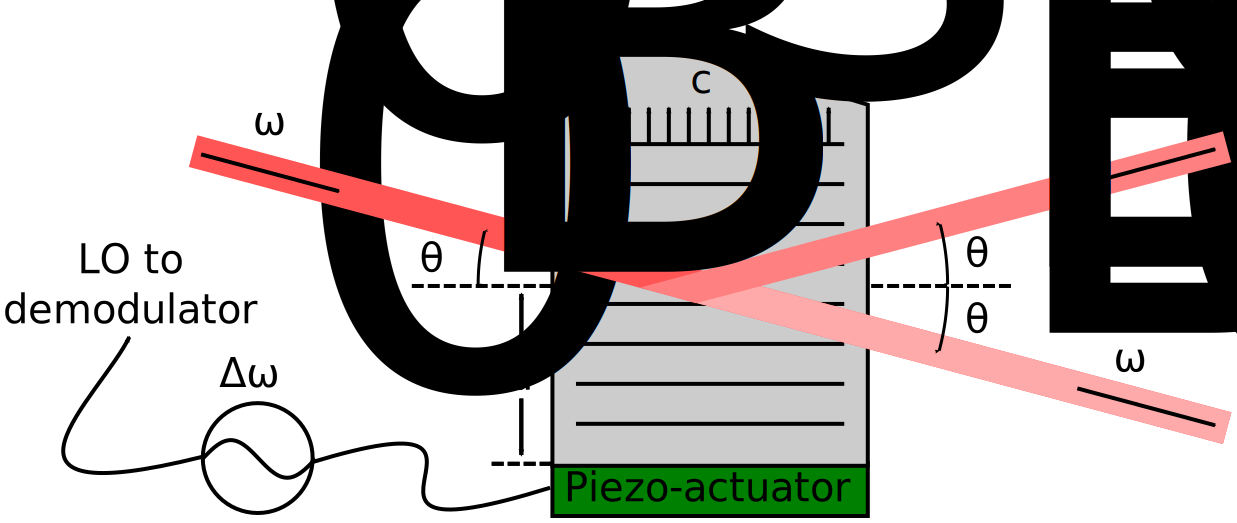
\includegraphics[width = \textwidth]{%
    Chapters/DesignConsiderations/figs/aom_scattering_diagram.pdf}
  \caption[Illustration of AOM operation in a heterodyne interferometer]{%
    An illustration of AOM operation in a heterodyne interferometer.
    A piezo-actuator drives sound waves of angular frequency $\Delta \omega_0$
    through a crystal (usually Germanium for $\SI{10.6}{\micro\meter}$ light),
    and these sound waves deflect and Doppler shift light
    that is incident upon the crystal at the Bragg angle $\theta_B$.
    The sound waves propagate from the piezo-actuator
    to the AOM's optically active region
    over finite time $\tau = d / c_s$.
    The RF waveform that drives the piezo-actuator
    is sampled and used to demodulate the heterodyne interference signal.
    Note that for simplicity the refraction of the beam
    as it enters and exits the crystal is \emph{not} depicted.}
\label{fig:DesignConsiderations:aom_scattering_diagram}
\end{figure}

The coupling of the AOM's drive signal to the deflected beam
occurs on the crystal's sound-wave timescale.
If the sound waves must propagate a distance $d$
from the piezo-actuator to the AOM's optically active region,
the drive signal is coupled to the deflected beam
only after time delay $\tau = d / c_s$.
\graffito{\textcolor{red}{reference?}}
The sound speed in Germanium is $c_s = \SI{5400}{\meter\per\second}$
such that a distance $d = \SI{1}{\centi\meter}$
is accompanied by a time delay $\tau = \SI{1.85}{\micro\second}$.
Note that this is large compared to many other timescales
typically considered in interferometry;
for example, light propagates
through $\SI{1}{\meter}$ of air
in only $\SI{3.33}{\nano\second}$,
and an RF signal propagates
through $\SI{1}{\meter}$ of RG-58 coaxial cable
(for which the index of refraction is $\sim 3 / 2$)
in only $\SI{5}{\nano\second}$.

In the presence of local-oscillator (LO) phase noise,
an AOM's finite coupling time
can degrade the performance of a heterodyne interferometer.
A local oscillator with phase noise is well-described by
\begin{equation}
  V_{\text{LO}}(t)
  =
  V_{0}
  e^{-i [\Delta \omega_0 t + \phi_{\Delta \omega_0}(t)]},
\end{equation}
where $\phi_{\Delta \omega_0}(t)$ is a zero-mean, stationary, random process
known as the LO's \emph{phase deviation}
whose temporal variation causes
the LO's instantaneous angular frequency
to wander about its nominal value $\Delta \omega_0$.
As discussed in the previous paragraph,
the AOM's finite coupling time far exceeds
the few tens of nanoseconds required for the beam
to propagate through an interferometer
of optical path length $\sim \SI{10}{\meter}$.
Thus, to account for the AOM's finite coupling time and
the local oscillator's jitter, take
$\Delta \omega_0 t
\rightarrow
[\Delta \omega_0 (t - \tau) + \phi_{\Delta \omega_0}(t - \tau)]$
in the heterodyne intensity
(\ref{eq:InterferometricMethods:heterodyne_intensity}).
Then, assuming negligible finite sampling-volume effects,
the heterodyne output voltage
from a detector element at position $\vect{r}_{\image}$
is simply proportional to the local intensity, i.e.\
\begin{align}
  \begin{aligned}
    V_{\text{het}}(\vect{r}_{\image}, t)
    &=
    2 V_0
    \bigl\{%
      1
      +
      \cos\left[%
        \Delta \omega_0 t
        +
        \bar{\phi}_{\text{eff}}
        +
        \phi_{\Delta \omega_0}(t - \tau)
      \right]
      \\
      &\quad-
      \tilde{\phi}(x_{\image}, t)
      \sin\left[%
        \Delta \omega_0 t
        +
        \bar{\phi}_{\text{eff}}
        +
        \phi_{\Delta \omega_0}(t - \tau)
      \right]
    \bigr\},
  \end{aligned}
\end{align}
where $\bar{\phi}_{\text{eff}} = \bar{\phi} - \Delta \omega_0 \tau$.
Then, following the same demodulation ``program'' used between
(\ref{eq:InterferometricMethods:heterodyne_interferometer_I_and_Q_intensity})
and
(\ref{eq:InterferometricMethods:heterodyne_total_fluctuating_intensity}),
the demodulated in-phase ($V_I$) and quadrature ($V_Q$) signals are defined as
\graffito{\textcolor{red}{Sign \& arg.\ of $\delta \phi_{\Delta \omega_0}$??}}
\begin{align}
  V_{I}(t)
  +
  i \cdot V_{Q}(t)
  &=
  \frac{1}{V_0}
  \langle
    V_{\text{LO}}(t)
    \cdot
    V_{\text{het}}(t)
  \rangle_{\Delta \omega_0}
  \notag \\
  &=
  V_0
  e^{i \bar{\phi}_{\text{eff}}}
  \left[
    \tilde{\phi}(x_{\image}, t)
    +
    \delta \phi_{\Delta \omega_0}(t - \tau, \tau)
  \right],
\end{align}
and the total fluctuating voltage in the demodulated signals is
\begin{equation}
  \tilde{V}_{IQ}(t)
  =
  V_0
  \left[
    \tilde{\phi}(x_{\image}, t)
    +
    \delta \phi_{\Delta \omega_0}(t - \tau, \tau)
  \right].
\end{equation}
Thus, the measured phase fluctuation
$\tilde{\phi}_{\text{meas}}(x_{\image}, t)
=
\tilde{V}_{IQ}(t) / V_0$
becomes
\graffito{\textcolor{red}{Sign \& arg.\ of $\delta \phi_{\Delta \omega_0}$??}}
\begin{equation}
  \tilde{\phi}_{\text{meas}}(x_{\image}, t)
  =
  \tilde{\phi}(x_{\image}, t)
  +
  \delta \phi_{\Delta \omega_0}(t - \tau, \tau);
\end{equation}
that is, the fluctuating signal is contaminated
by the local oscillator's phase noise.
The spectral properties of $\delta \phi_{\Delta\omega_0}(t, \tau)$
are thoroughly discussed in Appendix~\ref{app:OscillatorPhaseNoise}.
As $\delta \phi_{\omega_0}(t, \tau)$ and
$\tilde{\phi}(x_{\image}, t)$ are uncorrelated,
the autospectral density of the measured phase fluctuations is
\begin{equation}
    S_{\tilde{\phi}_{\text{meas}}}(f)
    =
    S_{\tilde{\phi}}(f)
    +
    8 \sin^2(\pi f \tau) \mathcal{L}_{\Delta\omega_0}(f),
\end{equation}
where $\mathcal{L}_{\Delta\omega_0}(f)$ is the phase noise of the LO,
as defined in Appendix~\ref{app:OscillatorPhaseNoise}.


\section{Amplitude noise: sources and effects}
\label{sec:DesignConsiderations:amplitude_noise}
Detector noise and shot noise are typically
the largest contributors to amplitude noise
in the heterodyne interference signal, while
a noisy amplifier can degrade the signal-to-noise ratio.
The demodulation of such amplitude noise
is throughly discussed by Rakhmanov in~\cite{rakhmanov_ao01}.
While Rakhmanov does not explicitly consider quadrature heterodyne detection,
his results can be naturally applied to quadrature heterodyne detection,
as is done below.


\subsection{Detector noise}
\graffito{\textcolor{red}{check signs and write more clearly}}
Real-world detector operation is associated with intrinsic noise.
This noise results from, among other things,
Johnson thermal noise in the detector and its associated electronics
and shot noise in the background radiation flux
\cite{hamamatsu_ir_detectors}.
A detector's noise is often characterized by
its noise-equivalent power ($NEP$):
when the power of the incident optical signal is equal to the $NEP$,
the signal-to-noise ratio is unity.
For a measurement with temporal bandwidth $\Delta f$,
a detector element with effective area $A$
will have an $NEP$
\begin{equation}
  NEP = \frac{\sqrt{A \cdot \Delta f}}{D^{*}},
\end{equation}
where $D^{*}$ is the detector's specific detectivity
\cite{jones_josa60}.
Note that larger $D^{*}$ corresponds to increased detector sensitivity.

Signal demodulation pushes detector noise
near the heterodyne frequency $\Delta \omega_0$
into the baseband signal, as is now demonstrated.
Note that
\begin{equation}
  NEP = \left\{ E\left[ \left| \delta P(t) \right|^2 \right] \right\}^{1/2},
\end{equation}
where $\delta P(t)$ is a real-valued, zero-mean, stationary, random process
that gives rise to the $NEP$ and
$E$ is the expectation-value operator.
Following a formalism similar to that from
Section~\ref{sec:InterferometricMethods:interferometry:heterodyne},
the detector noise in the in-phase ($I$) channel will be
\begin{equation}
  \delta P_I(t)
  =
  \left.
    \left[
      \cos(\Delta \omega_0 t) \cdot \delta P(t)
    \right]
  \right|_{|\omega| \ll \Delta \omega_0},
\end{equation}
and the detector noise in the quadrature ($Q$) channel will be
\begin{equation}
  \delta P_Q(t)
  =
  \left.
    \left[
      \sin(\Delta \omega_0 t) \cdot \delta P(t)
    \right]
  \right|_{|\omega| \ll \Delta \omega_0}.
\end{equation}
These two powers can be conveniently combined as
\begin{align}
  \delta P_{IQ}(t)
  &=
  \delta P_{I}(t) - i \cdot \delta P_{Q}(t)
  \notag \\
  &=
  \left.
    \left[
      e^{- i \Delta \omega_0 t} \cdot \delta P(t)
    \right]
  \right|_{|\omega| \ll \Delta \omega_0}.
\end{align}
Then, the autocorrelation function of corresponding baseband noise is
\begin{align}
  R_{\delta P_{IQ},\delta P_{IQ}}(\tau)
  &=
  E\left[\delta P_{IQ}(t) \cdot \delta P_{IQ}(t + \tau) \right]
  \notag \\
  &=
  e^{i \Delta \omega_0 \tau} \cdot R_{\delta P, \delta P}(\tau),
\end{align}
where $R_{\delta P, \delta P}(\tau)$ is the
autocorrelation function of the detector noise.
The corresponding autospectral density
of the demodulated detector noise is then
\begin{align}
  S_{\delta P_{IQ},\delta P_{IQ}}(\omega)
  &=
  \mathcal{F}\left[ R_{\delta P_{IQ},\delta P_{IQ}}(\tau) \right](\omega)
  \notag \\
  &=
  \mathcal{F}\left[
    e^{i \Delta \omega_0 \tau} \cdot R_{\delta P, \delta P}(\tau)
  \right](\omega)
  \notag \\
  &=
  S_{\delta P, \delta P}(\omega - \Delta \omega_0)
  \notag \\
  &\approx
  S_{\delta P, \delta P}(\Delta \omega_0),
  \label{eq:DesignConsiderations:detector_noise_demodulated}
\end{align}
\graffito{\textcolor{red}{$\sim \SI{e-18}{\watt\squared\per\hertz}$}}
where $S_{\delta P, \delta P}$ is
the autospectral density of the detector noise, and
the approximation follows from
the low-pass filtering
(i.e.\ $|\omega| \ll \Delta \omega_0$) and
the realness of $\delta P$
(i.e.\ $S_{\delta P, \delta P}(-\omega) = S_{\delta P, \delta P}(\omega)$).
That is, the detector noise at the heterodyne frequency $\Delta \omega_0$
is pushed into the baseband signal via the demodulation process.
Note that the autospectral density of the demodulated detector noise
(\ref{eq:DesignConsiderations:detector_noise_demodulated})
is in agreement with the literature
(e.g.\ see Rakhmanov's Eq.~(47) in~\cite{rakhmanov_ao01}
with $d_1 = 1 / 2$ for demodulation against a perfect sinusoid;
whereas Rakhmanov considers only \emph{one} of the demodulated channels,
(\ref{eq:DesignConsiderations:detector_noise_demodulated})
considers both the in-phase and quadrature channels and
is thus twice as large as Rakhmanov's expression).


\subsection{Shot noise}
The discrete nature of the arriving photons results in shot noise.
Well-modeled as a Poisson process,
the shot noise increases as $N_{\gamma}^{1/2}$, where
$N_{\gamma}$ is the number of incident photons.
Because the incident optical power (and hence the number of incident photons)
in the heterodyne optical signal is modulated as a function of time,
the corresponding shot noise is inherently \emph{nonstationary}.
Surprisingly, however, the demodulated shot noise \emph{is} stationary
(e.g.\ see Rakhmanov's Eq.~(59) in~\cite{rakhmanov_ao01}).
Note that Rakhmanov only considers \emph{one} of the demodulated signals, and
maximizing the signal-to-noise ratio in the demodulated signal
requires careful selection of the local oscillator's phase
relative to that of the heterodyne signal
(he terms this the ``demodulation phase'' and
represents it via $\gamma$).
However, by employing quadrature heterodyne detection~\cite{carlstrom_rsi88},
in which $\gamma_Q = \gamma_I + \pi / 2$,
the dependence on the demodulation phase vanishes; that is
\graffito{\textcolor{red}{$\sim \SI{e-21}{\watt\squared\per\hertz}$}}
\begin{align}
  S_{\delta P_{IQ}, \delta P_{IQ}}(\omega)
  &=
  S_{\delta P_{I}, \delta P_{I}}(\omega; \gamma_I)
  +
  S_{\delta P_{Q}, \delta P_{Q}}(\omega; \gamma_Q)
  \notag \\
  &=
  \hbar \omega_0 P_0,
\end{align}
where $\hbar$ is the Planck constant divided by $2 \pi$,
$\omega_0$ is the angular frequency of the incident photons, and
$P_0$ is the DC optical power impinging upon the detector.


\subsection{Amplifier noise}
The noise \emph{factor} $F$ of an RF amplifier is defined as the ratio of
the signal-to-noise ratio at the device's input ($SNR_{\text{in}}$) to
the signal-to-noise ratio at the device's output ($SNR_{\text{out}}$)
\begin{equation}
  F = \frac{SNR_{\text{in}}}{SNR_{\text{out}}};
\end{equation}
often, the noise factor $F$ is given
in terms of the noise \emph{figure} $NF$
\cite{minicircuits_amplifier_terms_defined}
\begin{equation}
  NF = 10 \log_{10} F.
\end{equation}
If several amplifiers are cascaded,
the total noise factor of the amplifier chain
can be computed using the well-known Friis noise-factor formula.
Note that the noise factor is only defined
in the context of a signal-to-noise ratio, so
it is not possible to write down the corresponding
autospectral density of the amplifier noise in absolute units.


\section{Demodulation}
\label{sec:DesignConsiderations:demodulation}
The interferometer's IF signal must be demodulated
in order to recover the baseband phase information.
Demodulation is typically described as an analog process
in which the IF signal is \emph{mixed} with a local oscillator (LO), but
demodulation can also be performed digitally
\cite{vanzeeland_rsi08, mlynek_fst12} or
with non-mixer-based analog electronics~\cite{mlynek_rsi17}.
The focus here, however, is on the analog-mixer-based approach.
Section~\ref{sec:DesignConsiderations:demodulation:ideal}
describes ideal analog demodulation.
Sections~\ref{sec:DesignConsiderations:demodulation:nonideal_mixing} and
\ref{sec:DesignConsiderations:demodulation:demodulator_imbalances}
discuss nonideal aspects of analog mixers and demodulators, and
Section~\ref{sec:DesignConsiderations:demodulation:imperfection_implications}
analyzes the implications of these imperfections
in the context of fluctuation measurements.


\subsection{Ideal demodulation}
\label{sec:DesignConsiderations:demodulation:ideal}
A typical analog $I\&Q$ demodulator consists of
a $90^{\circ}$ splitter,
two double-balanced mixers, and
a $0^{\circ}$ splitter~\cite{minicircuits_modulators}, as shown in
Fig.~\ref{fig:DesignConsiderations:analog_IQ_demodulator}(a).
The $90^{\circ}$ splitter divides the incident local oscillator (LO) signal
\begin{equation}
  \text{LO}(t) = \cos(\Delta\omega_0 t)
\end{equation}
into an ``in-phase'' copy of the LO
\begin{equation}
  \text{LO}_0(t)
  =
  \frac{1}{\sqrt{2}} \cos(\Delta\omega_0 t)
\end{equation}
and a $\pi / 2$-phase-advanced copy of the LO
\begin{equation}
  \text{LO}_{\pi / 2}(t)
  =
  \frac{1}{\sqrt{2}} \cos\left( \Delta\omega_0 t + \frac{\pi}{2} \right)
  =
  - \frac{1}{\sqrt{2}} \sin(\Delta\omega_0).
\end{equation}
Note that the power in the incident LO signal
is split evenly between $\text{LO}_0(t)$ and $\text{LO}_{\pi / 2}(t)$.
The $0^{\circ}$ splitter divides the intermediate frequency (IF) signal
\begin{equation}
  \text{IF}(t) = A_{\text{IF}} \cos(\Delta\omega_0 t + \phi)
  \label{eq:DesignConsiderations:IF_perfect_sinusoid}
\end{equation}
into two nominally identical copies of the IF
\begin{equation}
  \text{IF}_0(t)
  =
  \frac{A_{\text{IF}}}{\sqrt{2}} \cos(\Delta\omega_0 t + \phi).
\end{equation}
Like the LO signal, the power in the incident IF signal
is split evenly between the two copies.
The signal at the demodulator's in-phase ($I$) port
then corresponds to the product of
$\text{IF}_0(t)$ with the in-phase LO signal $\text{LO}_0(t)$:
\graffito{\textcolor{red}{incorrect amplitude}}
\begin{equation}
  \text{LO}_0(t) \cdot \text{IF}_0(t)
  =
  \frac{A_{\text{IF}}}{\sqrt{2}}
  \left[
    \cos(\phi) + \cos(2 \Delta\omega_0 t + \phi)
  \right].
\end{equation}
Such signal multiplication is often referred to as ``mixing''.
Low-pass filtering the signal exiting the demodulator's $I$ port
yields the baseband in-phase signal
\begin{equation}
  I = \frac{A_{\text{IF}}}{\sqrt{2}} \cos\phi.
\end{equation}
Similar reasoning regarding the product
$\text{LO}_{\pi / 2}(t) \cdot \text{IF}_0(t)$
at the demodulator's quadrature ($Q$) port
yields the baseband quadrature signal
\begin{equation}
  Q = \frac{A_{\text{IF}}}{\sqrt{2}} \sin\phi.
\end{equation}
Note that the total power in the $I\&Q$ signals
is $\SI{3}{\decibel}$ lower
than the power in the incident IF signal.
This is known as the \emph{conversion loss} of the demodulator, and
it results from low-pass filtering the $I\&Q$ signals;
real-world demodulators will have larger conversion losses
due to the additional effects of dissipation and other nonideal effects.
An \emph{absolute} phase measurement $\phi_m$ is then obtained via
\begin{equation}
  \phi_m = \atan\left( \frac{Q}{I} \right),
  \label{eq:DesignConsiderations:phase_from_arctangent}
\end{equation}
independent of the power in the incident IF signal.
Note that in the ideal case the measured phase is
equal to the true phase, i.e.\ $\phi_m = \phi$.

\begin{figure}
  \centering
  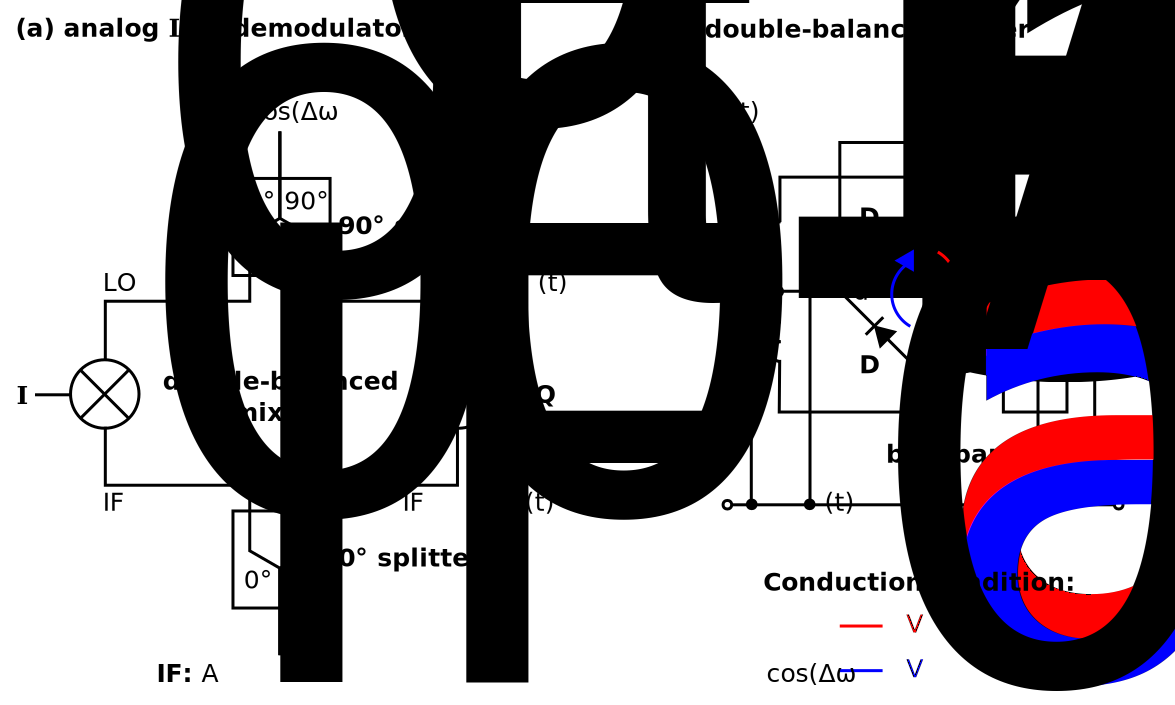
\includegraphics[width = \textwidth]{%
    Chapters/DesignConsiderations/figs/analog_IQ_demodulator.pdf}
  \caption[Components of a typical analog $I\&Q$ demodulator]{%
    (a) A typical analog $I\&Q$ demodulator and
    (b) a typical diode-ring double-balanced mixer.
    \textcolor{red}{Baseband??? More thorough descriptions}}
  \label{fig:DesignConsiderations:analog_IQ_demodulator}
\end{figure}


\subsection{Nonideal mixing}
\label{sec:DesignConsiderations:demodulation:nonideal_mixing}
In Section~\ref{sec:DesignConsiderations:demodulation:ideal},
mixing was idealized as the multiplication of the IF signal by the LO signal.
However, in practice, more complex process are used
to maximize the mixer's linear dynamic range and minimize its noise figure
\cite{analog_devices_mix_and_mod,bryant_mult_vs_mod}.

For example, a typical ring-diode double-balanced mixer
is shown in Fig.~\ref{fig:DesignConsiderations:analog_IQ_demodulator}(b).
The balun transformers $T_1$ and $T_2$
isolate the baseband port from the LO and IF ports.
Typically, the LO power is $\sim \SI{20}{\deci\bel}$ larger than the IF power.
As a result, the LO alone is responsible
for biasing the mixer's diodes into conduction.
Note that the diodes are not all simultaneously biased into conduction.
Instead, when $V_a > V_c$ (neglecting the diode drops),
diodes $D_1$ and $D_2$ are forced into conduction such that
$V_b$ acts as a virtual ground for the IF signal
coupled through transformer $T_2$.
Then, when the LO changes sign such that $V_a < V_c$,
diodes $D_1$ and $D_2$ stop conducting, and
diodes $D_3$ and $D_4$ begin to conduct,
forcing the virtual ground to jump from $V_b$ to $V_d$.
Thus, the ring diode acts as a switch
for the polarization of the coupled IF signal,
with the switching governed by the sign and frequency of the LO.
Low-pass filtering the polarization-modulated IF, of course,
yields the desired baseband signal.
Note that the diode switching time should be minimized
for optimal modulation,
explaining why some manufacturers
advocate the use of a square, rather than a sinusoidal, LO
\cite{minicircuits_mixer_faqs}.

\begin{figure}
  \centering
  \includegraphics[width = \textwidth]{%
    Chapters/DesignConsiderations/figs/LO_switching_function.pdf}
  \caption[LO switching functions]{%
    The LO switching functions.
    The top panel displays the incident sinusoidal LO signal, while
    the bottom panel shows the \emph{sign} of
    the in-phase ($\text{LO}_0$) and
    the $\pi / 2$ phase-advanced ($\text{LO}_{\pi / 2}$)
    copies of the LO signals.}
  \label{fig:DesignConsiderations:LO_switching_function}
\end{figure}

This polarization modulation can alter the baseband spectrum.
To see this, note that the sign of the in-phase LO signal
is simply a zero-mean square wave with even symmetry about the origin,
as shown in the lower pane of
Fig.~\ref{fig:DesignConsiderations:LO_switching_function}.
The Fourier series of such a square wave
consists of a sum over all of the LO's \emph{odd} harmonics:
\begin{align}
  \text{sgn}\left( \text{LO}_0(t) \right)
  &=
  \frac{4}{\pi}
  \sum_{n = 1}^{\infty}
  \frac{(-1)^{n - 1}}{2n - 1} \cos[(2n - 1) \Delta\omega_0 t]
  \\
  &\begin{aligned}
    =
    \frac{4}{\pi}
    \biggl[%
      \cos(\Delta\omega_0 t)
      &-
      \frac{1}{3} \cos(3 \Delta\omega_0 t)
      +
      \cdots
    \biggr].
  \end{aligned}
  \notag
\end{align}
Now, if the IF signal is a perfect sinusoid
as in (\ref{eq:DesignConsiderations:IF_perfect_sinusoid}),
following Section~\ref{sec:DesignConsiderations:demodulation:ideal}'s program
of mixing the LO with the IF and low-pass filtering yields
the desired in-phase baseband signal, e.g.\
\begin{align}
  I
  &=
  \bigl[%
    \text{sgn}\left( \text{LO}_0(t) \right)
    \cdot
    \text{IF}_0(t)
  \bigr]
  \biggr|_{\omega \ll \Delta\omega_0}
  \notag \\
  &=
  \frac{\sqrt{2} A_{\text{IF}}}{\pi} \cos\phi
\end{align}
However, if the path from the mixer's IF port to its baseband port
is not wholly linear
(and every real-world device exhibits \emph{some} degree of nonlinearity),
the IF signal contain contributions from its higher-order harmonics.
If this nonlinearity depends only on the magnitude of the IF
(for example, double-sided saturation or clipping of the signal),
only the odd harmonics of the fundamental will contribute, e.g.
\graffito{\textcolor{red}{Fourier phase too; comment about selecting phasing for simple expressions}}
\begin{equation}
  \text{IF}_0(t)
  =
  \sum_{n = 1}^{\infty}
  A_{2n - 1} \cos\left[ (2n - 1) (\Delta\omega_0 t + \phi) \right],
\end{equation}
where $A_n$ is
the Fourier coefficient of the $n\ts{th}$ harmonic.
Typically, $A_n$ decreases as $n$ increases, but
raising the IF amplitude drives more nonlinear interactions and
increases the power in the higher order harmonics relative to the fundamental.
Then,
following Section~\ref{sec:DesignConsiderations:demodulation:ideal}'s program
of mixing the LO with the IF and low-pass filtering yields
\begin{align}
  I
  &=
  \bigl[%
    \text{sgn}\left( \text{LO}_0(t) \right)
    \cdot
    \text{IF}_0(t)
  \bigr]
  \biggr|_{\omega \ll \Delta\omega_0}
  \notag \\
  &=
  \frac{2 A_1}{\pi}
  \left[%
    \cos\phi
    -
    \frac{1}{3}\left( \frac{A_3}{A_1} \right) \cos 3 \phi
    +
    \cdots
  \right].
\end{align}
That is, the higher order harmonics of the IF signal
\emph{beat} with the corresponding higher order harmonics
of the LO switching function
to produce harmonics in the baseband signal.
The coefficient $A_n / (n \cdot A_1)$ gives
the \emph{suppression} of the $n\ts{th}$ harmonic, and
it is typically expressed in decibels
referenced to the power of the carrier, or dBc, as
\begin{equation}
  \text{suppression of $n\ts{th}$ harmonic [dBc]}
  =
  20 \log_{10} \left( \frac{A_n}{n \cdot A_1} \right).
\end{equation}
Noting that $\text{sgn}(\text{LO}_{\pi / 2}(t))$
is an inverted, zero-mean square wave
with \emph{odd} symmetry about the origin,
as shown in the lower pane of
Fig.~\ref{fig:DesignConsiderations:LO_switching_function},
a similar path of reasoning to that used above
shows that the quadrature baseband signal is
\begin{align}
  Q
  &=
  \bigl[%
    \text{sgn}\left( \text{LO}_{\pi / 2}(t) \right)
    \cdot
    \text{IF}_0(t)
  \bigr]
  \biggr|_{\omega \ll \Delta\omega_0}
  \notag \\
  &=
  \frac{2 A_1}{\pi}
  \left[%
    \sin\phi
    +
    \frac{1}{3}\left( \frac{A_3}{A_1} \right) \sin 3 \phi
    +
    \cdots
  \right].
\end{align}
Additional distortion of the baseband signal results
if the IF power becomes comparable the LO power,
say within $\SI{10}{\deci\bel}$,
as the IF signal begins to contribute
to the modulation of the diode conduction.

Finally, the diodes of the mixers should be matched as closely as possible.
If, for example, diodes $D_1$ and $D_2$
have slightly different voltage drops than diodes $D_3$ and $D_4$,
the virtual grounds at $V_b$ and $V_d$ are not equivalent
when referenced to ground, and
a resulting baseband signal will have a DC offset.
\graffito{\textcolor{red}{Use percentage rather than dBc}}
With precision fabrication, however,
it is not uncommon for the DC offset to be $-60 \, \text{dBc}$
relative to the baseband fundamental harmonic.


\subsection{Demodulator imbalances}
\label{sec:DesignConsiderations:demodulation:demodulator_imbalances}
In addition to two double-balanced mixers,
an analog $I\&Q$ demodulator also relies on
a $90^{\circ}$ splitter and a $0^{\circ}$ splitter.
Imbalances between any of these components
can result in imbalances in the baseband $I\&Q$ signals.
For example, unequal power division in the splitters
produces amplitude imbalances in the baseband $I\&Q$ signals, while
deviations from the nominal splitter phasings
produces phase imbalances in the baseband $I\&Q$ signals.
As discussed in
Section~\ref{sec:DesignConsiderations:demodulation:nonideal_mixing},
each double-balanced mixer can produce
spectral distortion and DC offsets in the baseband signal;
in addition, differences between the two mixers
can exacerbate amplitude and phase imbalances
in the baseband $I\&Q$ signals.
Taken all together, then,
the most general form for the baseband $I\&Q$ signals is
\begin{align}
  I
  &=
  I_1 \left\{%
    \cos\phi
    -
    \frac{I_3}{3 I_1}
    \cos \left( 3 \phi \right)
    +
    \cdots
  \right\}
  +
  \delta I,
  \label{eq:DesignConsiderations:I_general}
  \\
  Q
  &=
  Q_1 \left\{%
    \sin \left( \phi + \delta \right)
    +
    \frac{Q_3}{3 Q_1}
    \sin \left[ 3 \left( \phi + \delta \right) \right]
    +
    \cdots
  \right\}
  +
  \delta Q,
  \label{eq:DesignConsiderations:Q_general}
\end{align}
where
$I_1$ is the amplitude of the in-phase signal's fundamental harmonic,
$I_3$ is the amplitude of the in-phase signal's third harmonic, and
$\delta I$ is the in-phase signal's DC offset.
Similar nomenclature applies to the quadrature signal.
The phase imbalance of the demodulator is $\delta$.
Amplitude imbalances occur when $I_1 \neq Q_1$.
The harmonic suppressions are typically comparable,
e.g.\ $|I_3 / I_1| \approx |Q_3 / Q_1|$.
Note that (\ref{eq:DesignConsiderations:I_general}) and
(\ref{eq:DesignConsiderations:Q_general})
generalize previous forms for the $I\&Q$ signals
\cite{vanzeeland_rsi04}.


\subsection{Effects of demodulator imperfections}
\label{sec:DesignConsiderations:demodulation:imperfection_implications}
Demodulator imperfections produce errors
in the measured phase~\cite{vanzeeland_rsi04,kasten_masters}.
Specifically, if the $I\&Q$ signals suffer from imbalances and nonlinearities,
as shown in (\ref{eq:DesignConsiderations:I_general}) and
(\ref{eq:DesignConsiderations:Q_general}),
then the measured phase $\phi_m$ computed via the inverse tangent formula
(\ref{eq:DesignConsiderations:phase_from_arctangent})
will \emph{not} correspond to the true phase $\phi$, e.g.\
\begin{equation}
  \phi_m = \phi + \delta \phi,
\end{equation}
where $\delta\phi$ is the error in the measured phase.
The phase error is a complicated, periodic function of the true phase,
i.e.\ $\delta\phi = \delta\phi(\phi)$~\cite{vanzeeland_rsi04}.
For small phase fluctuations $|\tilde{\phi}| \ll 1$
about an equilibrium phase $\bar{\phi}$,
the error $\delta\tilde{\phi}$ in the measured fluctuating phase
is simply the \emph{change} in the total phase error
between $\bar{\phi}$ and $\bar{\phi} + \tilde{\phi}$
\cite{kasten_masters}:
\begin{equation}
  \delta\tilde{\phi}
  =
  \delta\phi(\bar{\phi} + \tilde{\phi}) - \delta\phi(\bar{\phi})
  \approx
  \left[%
    \left. \frac{d(\delta\phi)}{d\phi} \right|_{\bar{\phi}}
  \right] \tilde{\phi}.
\end{equation}
Thus, the \emph{relative} error in the measured fluctuating phase is
\begin{equation}
  \frac{\delta\tilde{\phi}}{\tilde{\phi}}
  =
  \left. \frac{d(\delta\phi)}{d\phi} \right|_{\bar{\phi}}
  \label{eq:DesignConsiderations:relative_fluctuation_error}
\end{equation}
The $I\&Q$ Lissajous curves and
the relative errors in the measured fluctuating phase
that result from various demodulator imperfections
are displayed in
Fig.~\ref{fig:DesignConsiderations:effects_of_demodulator_imperfections}.
Obviously, each demodulator imperfection should be minimized
in order to minimize the relative error
in the measured fluctuating phase.

\begin{figure}
  \centering
  \includegraphics[width = \textwidth]{%
    Chapters/DesignConsiderations/figs/demodulator_imperfections.pdf}
  \caption[Effects of demodulator imperfections]{%
    Demodulator imperfections produce errors in the measured phase.
    The left column displays the Lissajous curves
    that result from plotting
    the quadrature $Q$ vs.\ in-phase $I$ signals, while
    the right column plots the relative error
    $\delta\tilde{\phi} / \tilde{\phi}$
    in the measured fluctuating phase
    as a function of the equilibrium phase $\bar{\phi}$.
    Each row examines a different demodulator imperfection.
  }
  \label{fig:DesignConsiderations:effects_of_demodulator_imperfections}
\end{figure}


\section{Quantization noise}
\label{sec:DesignConsiderations:quantization}
Efficient conversion of an analog signal to a digital record requires
quantization of the signal magnitude and
temporal sampling of these quantized magnitudes~\cite{bennett_bstj48}.
This analog-to-digital conversion
is performed by an instrument known as a digitizer.
If a digitizer has bit depth $N_b$ and
an input-voltage dynamic range $V_{\text{dyn}}$,
then its quantum of voltage $\Delta V$ is
\begin{equation}
  \Delta V
  =
  \frac{V_{\text{dyn}}}{2^{N_b} - 1}
  \approx
  \frac{V_{\text{dyn}}}{2^{N_b}},
  \label{eq:DesignConsiderations:digitizer_voltage_quantum}
\end{equation}
where the approximation is well-satisfied
for typical digitizer bit depths.
At each sampling time,
the analog signal's magnitude is approximated
by the closest quantized value, whose
separation from the true, analog value
will be less than or equal to $\Delta V / 2$.

In general, then, the quantized signal
will differ from the analog signal.
This error $\epsilon$ is known as quantization noise.
The mean square error (i.e.\ variance) attributable to quantization is simply
\begin{equation}
  \overline{\epsilon^2} = \frac{(\Delta V)^2}{12},
  \label{eq:DesignConsiderations:quantization_noise_variance}
\end{equation}
where $\Delta V$ is the digitizer's quantum of voltage,
as given by (\ref{eq:DesignConsiderations:digitizer_voltage_quantum})
\cite{bennett_bstj48}
\cite[Sec.~10.2.4]{bendat_and_piersol}.
For a uniformly sampled record with sampling rate $f_s$,
sufficiently fine quantization $\Delta V$
ensures that the quantization noise is \emph{white}
\cite[Th.~1]{bennett_bstj48}
\cite[Ch.~20]{widrow_and_kollar};
that is, the autospectral density of the quantization noise is
\begin{align}
  S_{\epsilon,\epsilon}(f)
  =
  \frac{\overline{\epsilon^2}}{f_s}
  =
  \frac{(\Delta V)^2}{12 f_s},
  \qquad
  -f_s < f \leq f_s.
  \label{eq:DesignConsiderations:quantization_noise_autospectral_density}
\end{align}
In practice, however, aperture error, jitter, and nonlinearities
may reduce the effective bit depth by one or two bits
\cite[Sec.~10.2.4]{bendat_and_piersol},
increasing the realized quantization noise
relative to that expected from
(\ref{eq:DesignConsiderations:quantization_noise_variance}) and
(\ref{eq:DesignConsiderations:quantization_noise_autospectral_density}).

Quantization noise can be significant
when attempting to measure absolute phase fluctuations
with a heterodyne interferometer.
Recall from the discussion of heterodyne interferometric detection in
Section~\ref{sec:InterferometricMethods:interferometry:heterodyne}
that measurement of the \emph{absolute} phase
requires capturing the full dynamics
of the large, slowly varying equilibrium phase $\bar{\phi}$
in addition to measurement of the fluctuating phase $\tilde{\phi}$.
Because $\tilde{\phi} \ll \bar{\phi}$ in typical situations,
the fluctuations only occupy a small portion
of the digitizer's dynamic range; that is,
fluctuations effectively see a bit depth that
is substantially smaller than the digitizer's nominal bit depth.
Thus, to minimize the effect of quantization noise,
it is absolutely imperative
to utilize the full dynamic range of the digitizer.


\bibliographystyle{plainurl}
\bibliography{references}
%
\chapter{Implementation of a combined PCI-interferometer on \diiid}


\section{Optical-diagnostic access on \diiid}
\label{sec:Implementation:d3d_ports}
\diiid \space provides optical access to its plasmas
through a number of ports, as indicated in
Fig.~\ref{fig:Implementation:d3d_port_locations}.
The ports are labeled according to their
toroidal positions and their sightlines, and
an experimentalist should have at least
a rough familiarity with these conventions.
The toroidal location of a port
is given in degrees clockwise from ``machine north''
when viewing the machine from above
(note that machine north does \emph{not} correspond
to geographic or magnetic north).
The angular separation of adjacent toroidal ports is $15^{\circ}$.
Port sightlines can be vertical or radial.
Ports with vertical (V) sightlines
are labeled sequentially in terms of increasing major radius,
with $V1$ having the smallest major radius and
$V3$ having the largest major radius.
Radial ports (R) have sightlines
that are roughly aligned with the plasma's minor radius, and
they are labeled according to their positions
relative to the plasma midplane:
R0 sits at the plasma midplane,
R+1 and R+2 are the first and second ports
\emph{above} the plasma midplane, respectively, and
R-1 and R-2 are the first and second ports
\emph{below} the plasma midplane, respectively.

\begin{figure}
  \centering
  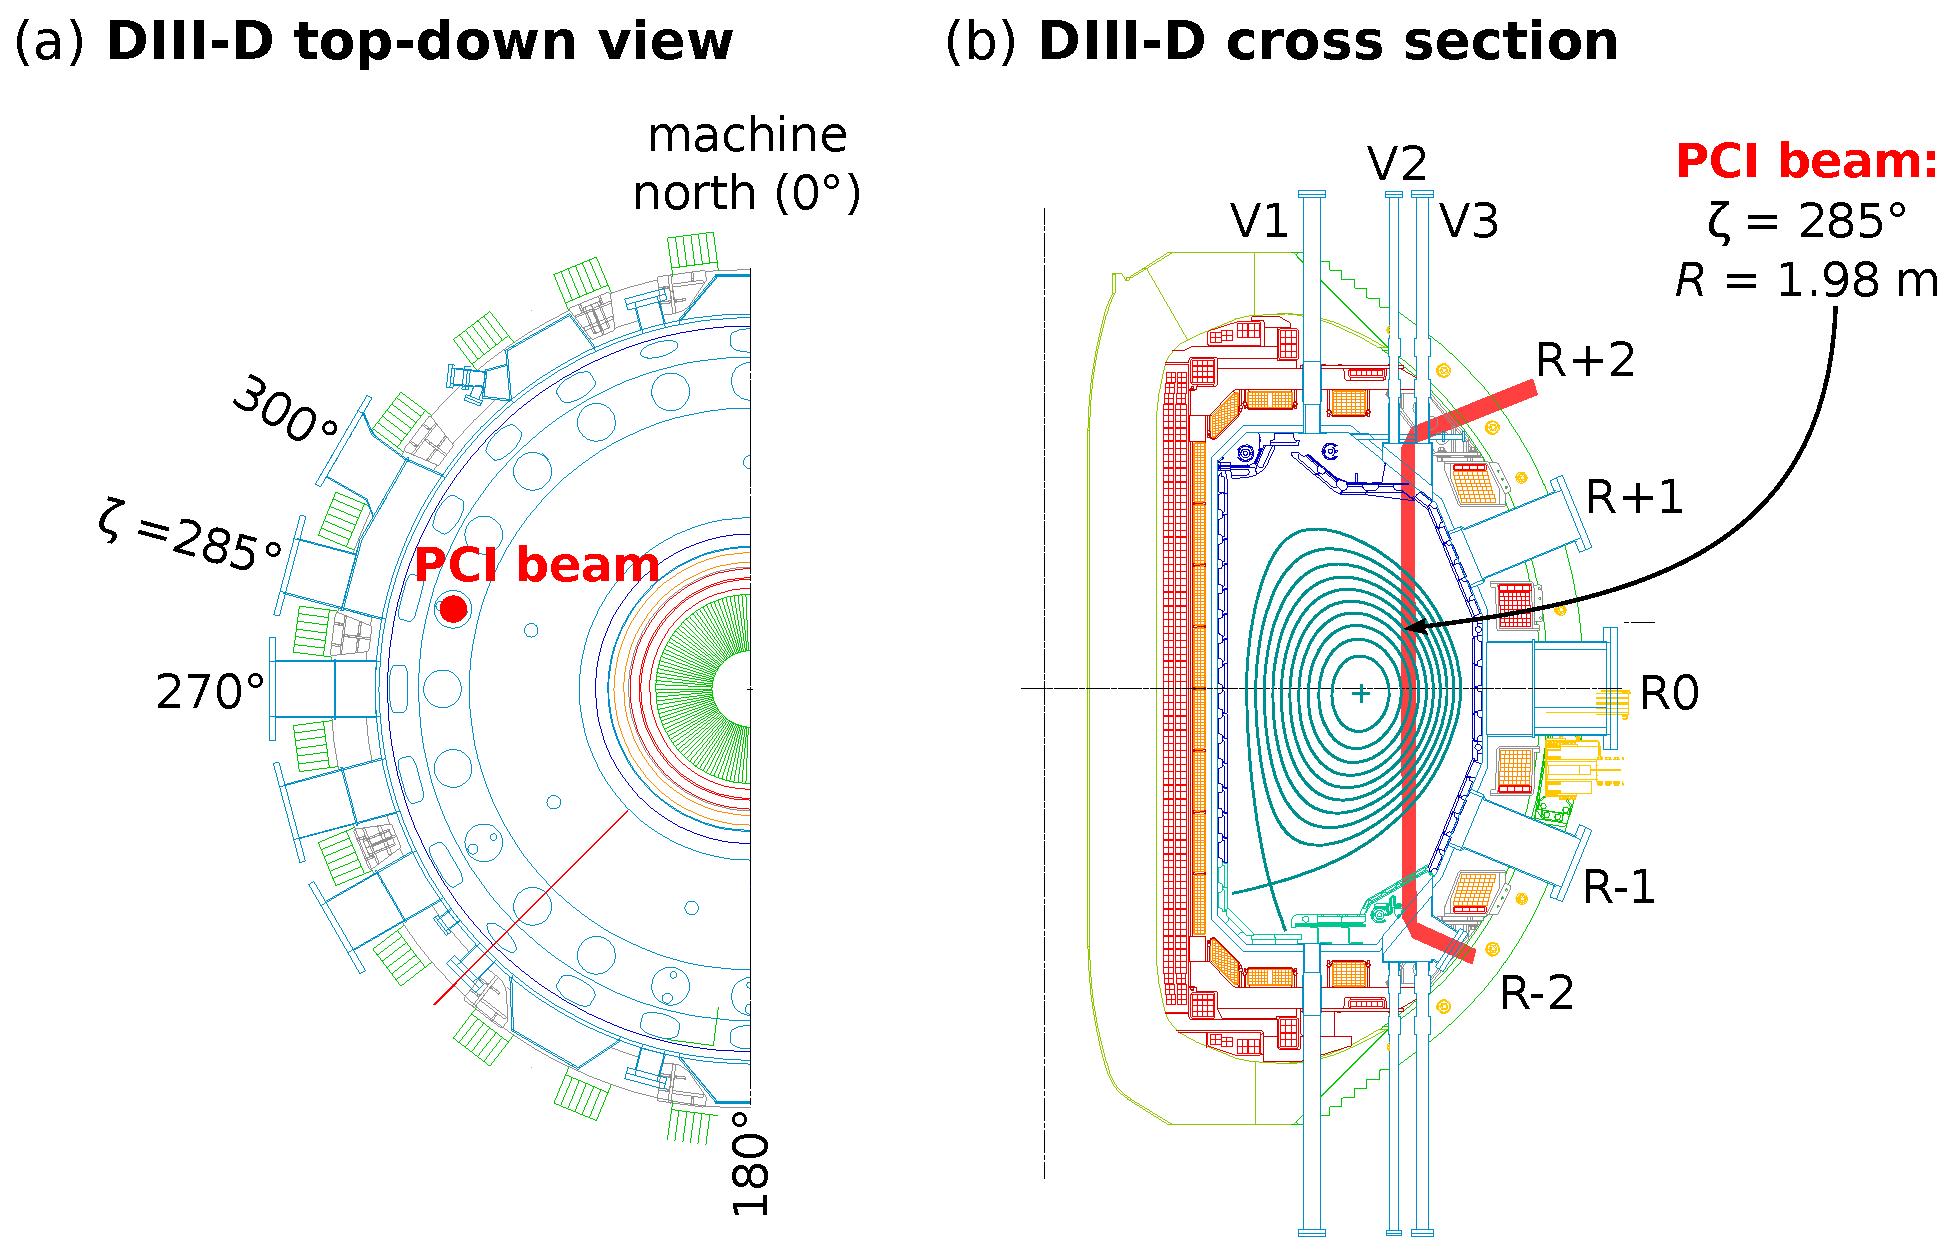
\includegraphics[width = \textwidth]{%
    Chapters/Implementation/figs/d3d_port_locations.pdf}
  \caption[\diiid \space port-labeling conventions and location of PCI]{%
    (a) View of \diiid \space from above,
    indicating the toroidal-labeling convention.
    (b) View of \diiid \space cross section,
    indicating the labeling convention
    for vertical (V) and radial (R) sightlines.
    The PCI beam enters the vessel through the $285^{\circ}$ R+2 port,
    propagates vertically downwards through the plasma
    at a major radius of $R = \SI{1.98}{\meter}$, and
    exits the vessel through the $285^{\circ}$ R-2 port.}
\label{fig:Implementation:d3d_port_locations}
\end{figure}


\section{\diiid's pre-existing PCI system}
The \diiid \space PCI system is
thoroughly described elsewhere~\cite{dorris_rsi09, dorris_phd}, but
the system components of relevance to this work
are briefly summarized below for completeness.


\subsection{System geometry}
The system is currently configured
in the ``Phase II'' geometry~\cite{dorris_rsi09},
with the probe beam propagating vertically downwards
from the $285^{\circ}$ R+2 port to the $285^{\circ}$ R-2 port.
The beam center sits at $R = $ \SI{1.98}{\meter}.
Both the toroidal and radial positions
of the PCI beam are shown in
Fig.~\ref{fig:Implementation:d3d_port_locations}.

The PCI system's vertical beam path constrains
which types of fluctuations it can and cannot detect.
Namely, the PCI-measured power fluctuations
(\ref{eq:InterferometricMethods:PCI_ratio_fluctuating_to_equilibrium_power})
correspond to \emph{line-integrated} electron-density fluctuations, which
are the physical origin of the phase fluctuations $\tilde{\phi}$ in
(\ref{eq:InterferometricMethods:phase_fluctuation}).
Because it is a line-integrated measurement,
only fluctuations propagating perpendicular to the beam path can be detected,
as fluctuations propagating parallel to the beam path
are effectively averaged out of the signal
\graffito{\textcolor{red}{what about $\delta \omega$?}}
(and, at a more fundamental level, fluctuations propagating
parallel to the beam path do \emph{not} spatially scatter the probe beam).
\graffito{\textcolor{red}{citation? Wesson?}}
Now, electrostatic turbulence (e.g.\ ITG, ETG) tends to be field-aligned
such that $k_{\perp} \gg k_{||}$, where
the $\perp$ and $||$ subscripts are used here to indicate
orientations that are perpendicular to and parallel to
the local magnetic field, respectively.
To lowest order, then, electrostatic fluctuations propagate
perpendicular to a tokamak's toroidal field.
PCI's vertical beam path and
the field-aligned constraint of electrostatic turbulence
imply that PCI is predominantly sensitive to fluctuations
with finite major-radial wavenumber $k_R$.
Thus, PCI's 32-element, 1-dimensional detector array
is oriented in the image plane such that
each detector element corresponds to a unique major radius in the plasma.

In some situations, 2-dimensional detector arrays
\cite{sanin_rsi04, tanaka_rsi16} or
spatially filtering ``masks''~\cite{dorris_rsi09, dorris_phd, lin_rsi06}
can be used to localize measurements
by exploiting the spatial variation
in the magnetic field's orientation along the beam path.
These localization techniques typically work best
for high-$k$ measurements.
Note that $k_R$ is related to the
often-theoretically-relevant poloidal wavenumber $k_{\theta}$ via
\begin{equation}
  k_R = k_{\theta} \csc[\alpha(R, z)],
  \label{eq:Implementation:kR_to_ktheta}
\end{equation}
where $\alpha(R, z)$ is the angle
between the beam path and the local flux surface,
as shown schematically in
Fig.~\ref{fig:Implementation:relating_kR_to_ktheta}.
Of course, the fluctuation measurements must be localized,
either via direct measurement
(with 2-dimensional detector arrays or ``masks'')
or via inference from other plasma properties,
before (\ref{eq:Implementation:kR_to_ktheta})
can be inverted to yield $k_{\theta}$
from measured values of $k_R$.

\begin{figure}
  \centering
  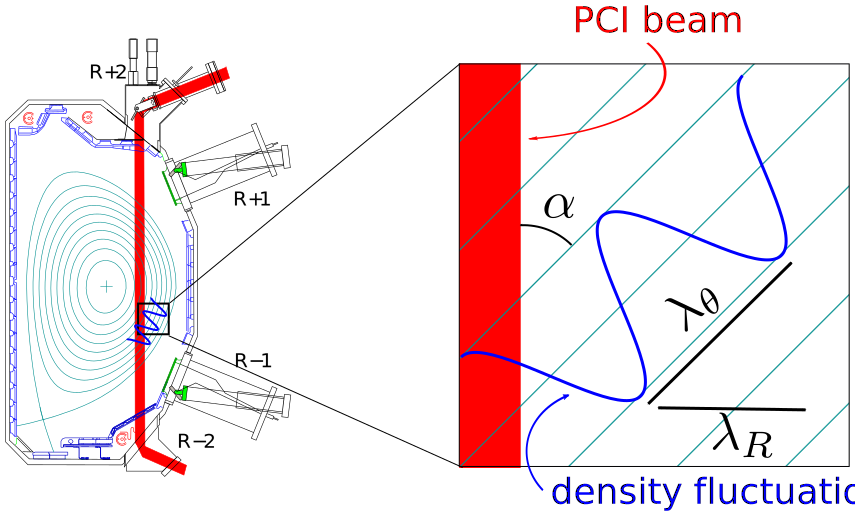
\includegraphics[width = 0.9 \textwidth]{%
    Chapters/Implementation/figs/kR_to_ktheta.pdf}
  \caption[Relating $k_R$ to $k_{\theta}$]{%
    The major-radial wavenumber $k_R = 2 \pi / \lambda_R$ and
    the poloidal wavenumber $k_{\theta} = 2 \pi / \lambda_{\theta}$
    are related via $\alpha(R, z)$, which
    is the angle between PCI's vertical probe beam and
    the local flux surface.}
\label{fig:Implementation:relating_kR_to_ktheta}
\end{figure}


\subsection{Spatial bandwidth}
The system has $k_{\text{min}}^{\text{PCI}} = \SI{1.5}{\per\centi\meter}$.

The 1/e electric field radius of the in-vessel beam is
$w_0 =$ \SI{3.4}{\centi\meter}, and

A pair of fast steering mirrors dynamically centers
the unscattered beam on the phase plate groove,
compensating for vibrations.



\subsection{Temporal bandwidth}


\begin{itemize}
  \item $k$-cutoff
  \item Maintenance
    \begin{itemize}
      \item Replacement of laser
      \item Replacement of feedback detector
      \item Replacement of in-vessel mirrors
    \end{itemize}
\end{itemize}

\section{Interferometer design}
\begin{itemize}
  \item Power sharing between the interferometer arms and PCI
  \item TE-cooled detector
  \item Imaging and $k$-response
  \item Demodulation scheme
\end{itemize}

\section{Interferometer optimization}
\begin{itemize}
  \item LO stability
  \item External clock
\end{itemize}

\section{Sound-wave calibration of combined PCI-interferometer}
\begin{itemize}
  \item Importance of speaker placement
  \item System sensitivity
\end{itemize}


\bibliographystyle{plainurl}
\bibliography{references}
%
\chapter{Correlation of \diiid's toroidally separated interferometers}
The toroidal structure of an MHD mode can strongly influence
the mode's stability and its interaction with the surrounding plasma.
A mode's toroidal structure is typically characterized
via the toroidal mode number $n$.
Historically, measurement of toroidal (and poloidal) mode numbers
with magnetic loops has provided rich insight
into the physics governing numerous operational regimes and stability limits.
However, core-localized MHD produces weak signals outside of the plasma volume,
making measurement of mode numbers via magnetic loops difficult or impossible.
Recently, measurements from toroidally separated
electron cyclotron emission imaging (ECEI) systems
on the KSTAR tokamak have identified mode numbers of
edge-localized modes~\cite{lee_rsi_2014} and
sawteeth~\cite{choe_nf_2015},
raising the question as to the utility of using more exotic measurements
to probe the structure of core-localized MHD.

This chapter describes the use of toroidally separated interferometers
to measure toroidal mode numbers.
To the author's knowledge, this is the first such implementation in a tokamak.
The addition of the heterodyne interferometer channel
to \diiid's pre-existing phase contrast imaging (PCI) system
enabled this novel measurement.
As shown in Fig.~\ref{fig:ToroidalCorrelation:pci_interf_locs}
the beampaths of the PCI and V2 interferometers
are toroidally separated by $\Delta \zeta = 45^{\circ}$ and
are very nearly radially overlapping.
Section~\ref{sec:ToroidalCorrelation:two_point_correlations}
reviews the mathematics of the two-point-correlation technique
used to extract toroidal mode numbers and
derives the resulting Nyquist mode number.
Section~\ref{sec:ToroidalCorrelation:interferometer_measurements}
examines the interferometer measurements in detail and
develops a formula for the measured toroidal mode number.
Section~\ref{sec:ToroidalCorrelation:nonideal_effects}
characterizes the effects of time-base offsets and radial offsets
between the two interferometer systems and
describes methods to minimize their influence
on the measured toroidal mode number.

\begin{figure}
  \centering
  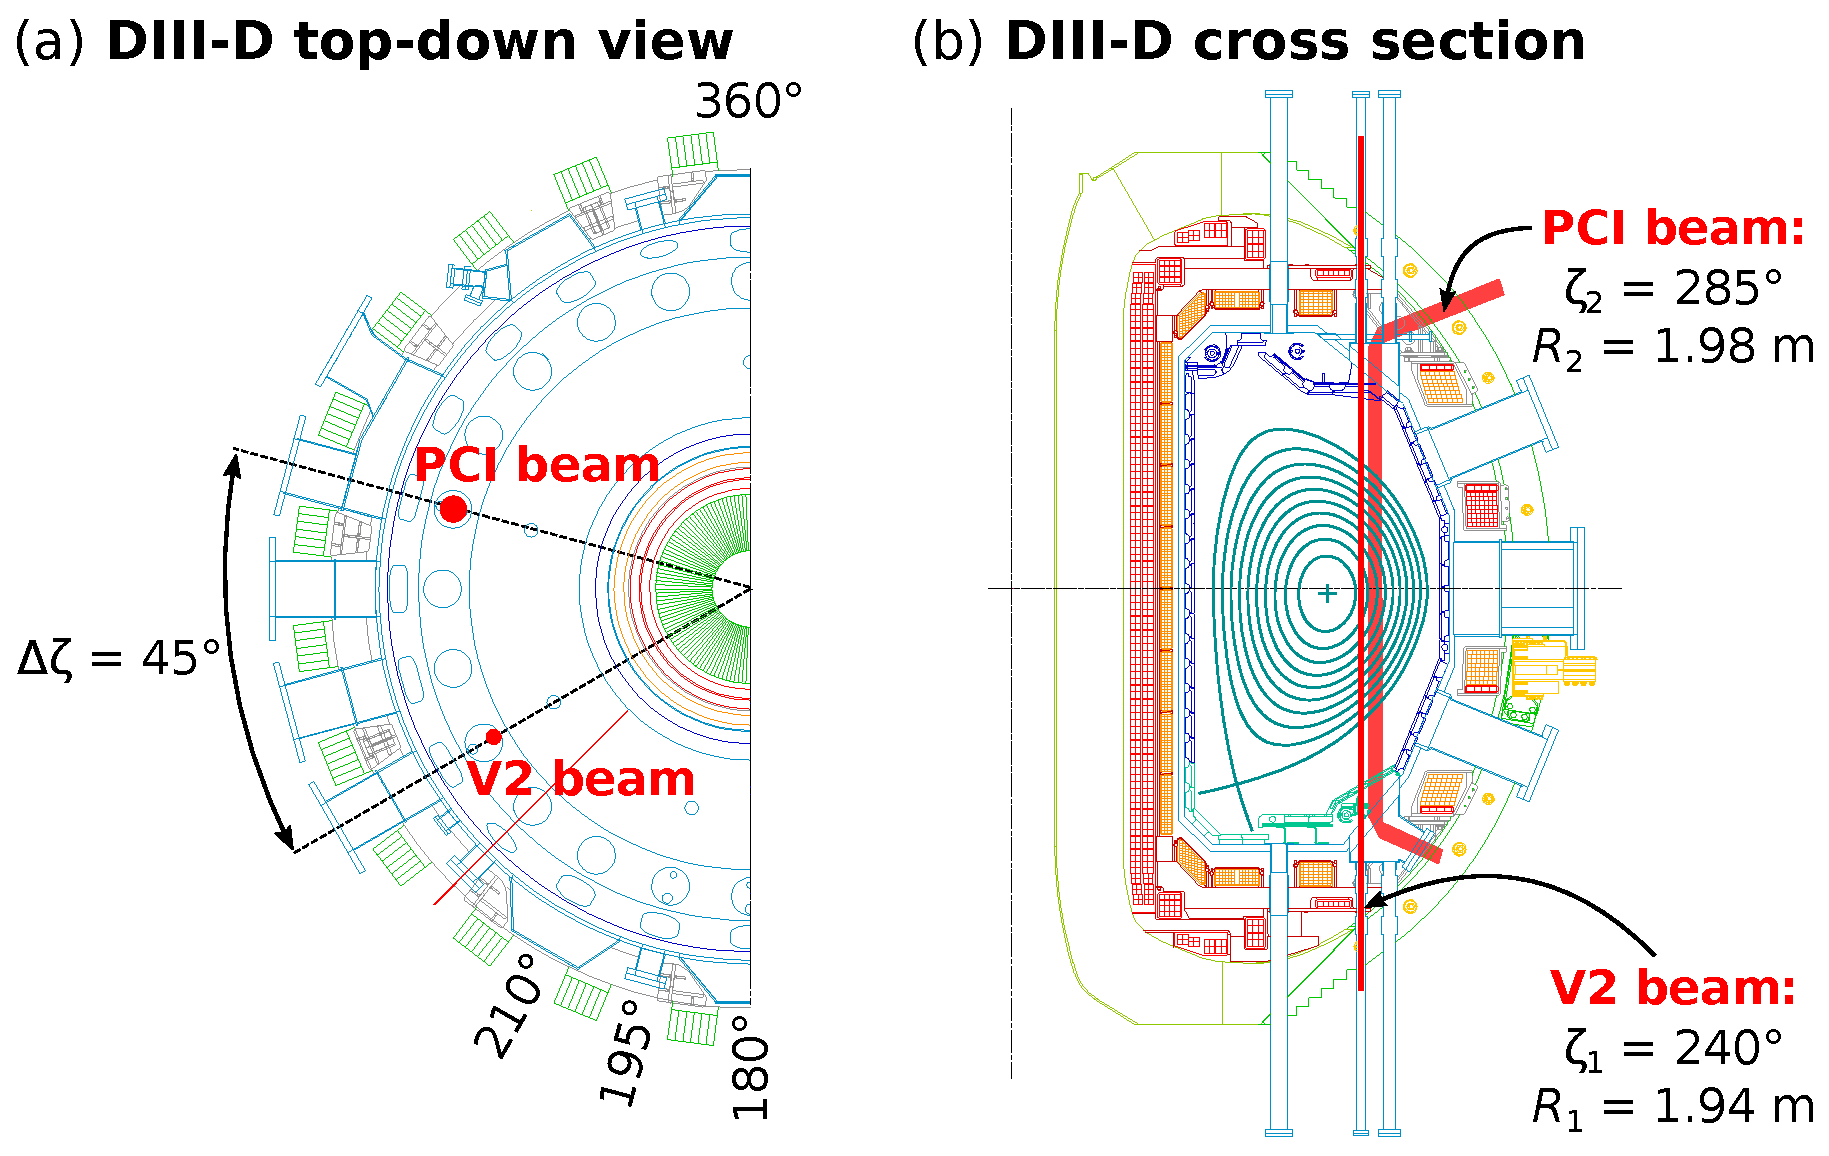
\includegraphics[width = \textwidth]{%
    Chapters/ToroidalCorrelation/figs/pci_interf_locs.eps}
  \caption[Beam locations of the V2 interferometer and PCI systems on \diiid]{%
    (a) A top-down view of the \diiid\space vessel.
    The V2 interferometer beam's toroidal location is $\zeta_1 = 240^{\circ}$,
    and the PCI beam's toroidal location is $\zeta_2 = 285^{\circ}$.
    (b) A view of the \diiid\space cross section.
    The V2 interferometer beam's
    major-radial location is $R_1 = \SI{1.94}{\meter}$, and
    the PCI beam's major-radial location is $R_2 = \SI{1.98}{\meter}$.}
\label{fig:ToroidalCorrelation:pci_interf_locs}
\end{figure}


\section{Two-point correlations}
\label{sec:ToroidalCorrelation:two_point_correlations}


\subsection{Spectral characterization of random processes}
In contrast to deterministic processes,
random processes cannot be modeled via an explicit mathematical relationship.
Rather, random processes are characterized
in terms of probabilities and statistical properties.
Any given observation of a random process represents
only one of many possible observations;
each such observation is referred to as
a ``sample'' or a ``realization'' of the random process
and is denoted as $x_k(t)$.
The random process itself consists of
the ensemble of all of the potential observations
and is denoted as $\{x_k(t)\}$.
Random processes can be stationary or nonstationary.
The statistical properties of a stationary random process
do not vary in time, and
the spectral tools discussed below
were all developed for analysis of stationary random processes.

The \emph{finite} Fourier transform $X_k(f, T)$
of a continuous signal $x_k(t)$ is defined as
\begin{equation}
  X_k(f, T)
  =
  \int_{-T / 2}^{T / 2}
  dt \, x_k(t) e^{-i \, 2 \pi f t}
  \label{eq:ToroidalCorrelation:finite_Fourier_transform}
\end{equation}
Note that $x_k(t)$ need \emph{not} be integrable over the infinite domain,
making the finite Fourier transform a suitable tool for stationary signals,
whose statistical properties (e.g.\ mean, variance, etc.) are
constant and potentially finite in time.

For real-valued, stationary random processes $\{x_k(t)\}$ and $\{y_k(t)\}$,
the one-sided cross-spectral density function $G_{xy}(f)$ is defined as
\begin{equation}
  G_{xy}(f)
  \equiv
  \lim_{T \rightarrow \infty}
  \frac{2}{T} E \left[ X_k^*(f, T) Y_k(f, T) \right]
  \label{eq:ToroidalCorrelation:cross_spectral_density_defn}
\end{equation}
for $0 < f < \infty$;
$G_{xy}(f)$ is not defined for $f < 0$, and
it is reduced by a factor of two relative to
(\ref{eq:ToroidalCorrelation:cross_spectral_density_defn}) at $f = 0$
(the value of $G_{xy}(0)$ is of little relevance to this work).
Note that $E[\cdot]$ is the expectation value operator;
this operator averages over all of the realizations in the ensemble, and
its application ensures that
(\ref{eq:ToroidalCorrelation:cross_spectral_density_defn})
is a statistically consistent definition of the cross-spectral density
(that is, ensemble averaging is needed for $G_{xy}(f)$
to approach the true cross-spectral density as $T \rightarrow \infty$).
In general $G_{xy}(f)$ is a complex-valued function;
this can be explicitly written as
\begin{equation}
  G_{xy}(f) = \left| G_{xy}(f) \right| e^{i \alpha_{xy}(f)}
  \label{eq:ToroidalCorrelation:cross_spectral_density_explicit_complex}
\end{equation}
where $\alpha_{xy}(f)$ is the \emph{phase angle}.
For the special case $\{x_k(t)\} = \{y_k(t)\}$,
$G_{xx}(f)$ is real-valued (i.e.\ $G_{xx}(f) = |G_{xx}(f)|$) and
is referred to as the one-sided autospectral density function.

The degree of correlation between random processes
$\{x_k(t)\}$ and $\{y_k(t)\}$ can be easily quantified
with the corresponding spectral density functions.
In particular, the magnitude-squared coherence function
$\gamma_{xy}^2(f)$ is defined as
\begin{equation}
  \gamma_{xy}^2(f)
  \equiv
  \frac{|G_{xy}(f)|^2}{G_{xx}(f) G_{yy}(f)}
  \label{eq:ToroidalCorrelation:magnitude_squared_coherence_defn}
\end{equation}
and it satisfies
\begin{equation}
  0 \leq \gamma_{xy}^2(f) \leq 1
  \label{eq:ToroidalCorrelation:magnitude_squared_coherence_bounds}
\end{equation}
for $0 \leq f < \infty$, with
$\gamma_{xy}^2(f) = 1$ indicating that
$\{x_k(t)\}$ and $\{y_k(t)\}$ are 100\% correlated at frequency $f$ and
$\gamma_{xy}^2(f) = 0$ indicating that
$\{x_k(t)\}$ and $\{y_k(t)\}$ are completely uncorrelated at frequency $f$.
Note that the ensemble-averaging operation in
(\ref{eq:ToroidalCorrelation:cross_spectral_density_defn})
is paramount to the computation
of \emph{informative} values for $\gamma_{xy}^2(f)$;
that is, if ensemble averaging is ignored, and
only single realizations of the random processes are used,
$\gamma_{xy}^2(f) \equiv 1$ for all $f$,
\emph{regardless} of the actual degree of coherence
between between $\{x_k(t)\}$ and $\{y_k(t)\}$.

Care should be taken when computing spectral densities.
In various programming languages,
it is not uncommon to ``detrend'' realizations $x_k(t)$ and $y_k(t)$
by subtracting the signal mean or linear trend
prior to application of
(\ref{eq:ToroidalCorrelation:cross_spectral_density_defn}).
However, the author has empirically found that
such detrending can lead to values of $\gamma_{xy}^2(f)$
that unphysically exceed the bounds established in
(\ref{eq:ToroidalCorrelation:magnitude_squared_coherence_bounds}).
The author has not explored more exotic means of detrending, and
no detrending was applied to signals prior to spectral computations
in this work.


\subsection{Nyquist mode number}


\section{Toroidal correlation of interferometers}
\label{sec:ToroidalCorrelation:interferometer_measurements}


\subsection{\diiid's interferometers}


\subsection{Perturbed plasma density}
An MHD mode displaces a plasma from it's equilibrium position
by $\vect{\xi} = \vect{\xi}(\vect{r}, t)$.
The perturbed velocity is given as
$\vect{v_1} = \partial \vect{\xi} / \partial t$
and, assuming harmonic variations, reduces to
\begin{equation}
  \vect{v_1}
  \equiv
  \frac{\partial \vect{\xi}}{\partial t}
  =
  -i \omega \vect{\xi}
  \notag
\end{equation}
where $\omega$ is the mode's angular frequency.
The plasma density $n_i$ is given as
\begin{equation}
  n_i = \bar{n}_i + \tilde{n}_i
  \notag
\end{equation}
where $\bar{n}_i$ and $\tilde{n}_i$ are
the equilibrium and fluctuating components, respectively.
Assuming a stationary equilibrium ($\vect{v_0} = 0$) and
using the above relations,
the linearized continuity equation reduces to
\begin{equation}
  \tilde{n}_i = -\nabla \cdot (\bar{n}_i \vect{\xi})
  \label{eq:ToroidalCorrelation:density_fluctuations}
\end{equation}
If we relax the assumption on $\vect{v_0}$ to allow
finite equilibrium flow ($\vect{v_0} \neq 0$),
then the right-hand side of (\ref{eq:ToroidalCorrelation:density_fluctuations})
is simply multiplied by the prefactor
$[1
- (\vect{v_0} \cdot \vect{k} / \omega)
+ i (\nabla \cdot \vect{v_0} / \omega)]^{-1}$, where
$\vect{k}$ is the mode wavevector.


\subsection{Interferometer-measured phase fluctuations}
For a CO$_2$ laser beam ($\lambda_0 =$ \SI{10.6}{\micro \meter})
in a tokamak plasma, the index of refraction $N$ is
\begin{equation}
  N
  \approx
  1 - \frac{1}{2} \left( \frac{\omega_{pe}}{\omega_0} \right)^2
  \notag
\end{equation}
where $\omega_{pe}$ is the electron angular plasma frequency and
$\omega_0 = 2 \pi c / \lambda_0 = 2 \pi \cdot \SI{28.3}{\tera\hertz}$
is the laser's angular frequency.
Thus, a CO$_2$ beam propagating through a tokamak plasma
will acquire a phase shift $\phi$ \emph{relative} to vacuum
\begin{equation}
    \phi
    =
    \frac{\omega}{c} \int (N - 1) dl
    =
    - r_e \lambda_0 \int n_e dl \notag
\end{equation}
where $r_e = \SI{2.8e-15}{\meter}$ is the classical electron radius.
Further, if there are electron density fluctuations $\tilde{n}_e$
about the equilibrium $\bar{n}_e$, there will be corresponding
phase fluctuations $\tilde{\phi}$
\begin{align}
  \tilde{\phi} = -r_e \lambda_0 \int \tilde{n}_e dl
  \label{eq:ToroidalCorrelation:phase_fluctuations_generic}
\end{align}
Assuming quasineutrality $n_e \approx n_i$ and
invoking (\ref{eq:ToroidalCorrelation:density_fluctuations}),
the phase fluctuations reduce to
\begin{align}
  \tilde{\phi}
  =
  r_e \lambda_0
  \int [\nabla \cdot (\bar{n}_e \vect{\xi})] dl
  \label{eq:ToroidalCorrelation:phase_fluctuations_from_displacement}
\end{align}

Now, \diiid's V2 and PCI interferometers have \emph{vertical} beam paths
located at major radial ($R$) and toroidal ($\zeta$) coordinates
$(R_1, \zeta_1) = (\SI{1.94}{\meter}, \; 240^{\circ})$ and
$(R_2, \zeta_2) = (\SI{1.98}{\meter}, \; 285^{\circ})$, respectively.
Fourier decomposing the displacement $\vect{\xi}$ as
\begin{equation}
  \vect{\xi}(\vect{r}, t)
  =
  \vect{\xi_0}(r) e^{i(m \theta + n \zeta - \omega t)}
  \notag
\end{equation}
for poloidal ($m$) and toroidal ($n$) mode numbers and
$\vect{\xi_0}(r) \in \mathbb{R}^3$,
(\ref{eq:ToroidalCorrelation:phase_fluctuations_from_displacement}) becomes
\begin{align}
  \tilde{\phi}
  =
  r_e \lambda_0
  \int \left\{
    \nabla
    \cdot
    \left[
      \bar{n}_e \, \vect{\xi_0}(r) e^{i(m \theta + n \zeta - \omega t)}
    \right]
  \right\} dl
  \notag
\end{align}
Finally, noting that $dl = dl(r, \theta)$ for vertical beam paths,
the phase fluctuations reduce to
\begin{equation}
  \tilde{\phi}
  =
  \Phi e^{i(n \zeta - \omega t)}
  \label{eq:ToroidalCorrelation:phase_fluctuations_vertical_beam1}
\end{equation}
where
$\Phi
\equiv
\Phi(R, m, n, \vect{\xi_0}(r), \bar{n}_e(r), \vect{G}) \in \mathbb{C}$
is a complex-valued function of
the beam's major radial location,
the mode structure,
the equilibrium density profile, and
the plasma geometry $\vect{G} = \vect{G}(R_0, a, \kappa, \delta, \cdots)$.
$\Phi$ can be written explicitly
as a complex value $\Phi = |\Phi| e^{i \sigma}$.

For a given mode and plasma,
the V2 and PCI interferometer beams see the \emph{same}
$\{m, n, \vect{\xi_0}(r), \bar{n}_e(r), \vect{G}\}$, and
$\Phi$ reduces to a one-dimensional function $\Phi = \Phi(R)$.
Thus, (\ref{eq:ToroidalCorrelation:phase_fluctuations_vertical_beam1}) can
alternatively be written as
\begin{equation}
  \tilde{\phi}
  =
  |\Phi(R)| e^{i[n \zeta - \omega t + \sigma(R)]}
  \label{eq:ToroidalCorrelation:phase_fluctuations_vertical_beam2}
\end{equation}
where the dependence on $R$ for a given mode and plasma
has been noted explicitly.
The phase angle $\alpha$ of $\tilde{\phi}$ is defined as
\begin{equation}
  \alpha \equiv n \zeta - \omega t + \sigma(R)
  \label{eq:ToroidalCorrelation:phase_angle}
\end{equation}
such that $\tilde{\phi} = |\Phi| e^{i \alpha}$.


\subsection{The measured mode number --- the ideal case}
In the ideal case, phase fluctuations $\tilde{\phi}_1$ and $\tilde{\phi}_2$
are made at different toroidal locations $\zeta_1 \neq \zeta_2$ but
the \emph{same} radial locations $R_1 = R_2 = R$.
The one-sided cross-spectral density
$G_{12}(f) = |G_{12}(f)| e^{i \alpha_{12}(f)}$
then yields an estimate of the relative phase angle
$\alpha_{12} \equiv \alpha_2 - \alpha_1 = n(\zeta_2 - \zeta_1)$,
inspiring the definition of the measured toroidal mode number as
\begin{equation}
  n_{\text{meas}}
  \equiv
  \frac{\alpha_{12}}{\Delta \zeta}
  \quad \text{where} \quad
  \Delta \zeta \equiv \zeta_2 - \zeta_1
  \label{eq:ToroidalCorrelation:toroidal_mode_number_ideal}
\end{equation}


\section{Non-ideal effects}
\label{sec:ToroidalCorrelation:nonideal_effects}
Offsets in the time bases and major radial positions
of the V2 and PCI interferometers can bias
the measured toroidal mode number
(computed via (\ref{eq:ToroidalCorrelation:toroidal_mode_number_ideal}))
away from the true toroidal mode number $n$.
Each effect is treated independently below.
While the time-base offset between the two systems
has now been measured (as discussed below) and compensated for,
accounting for the radial offset of the beams requires
forward modeling/synthetic diagnostics and a bit of intuition.


\subsection{Time-base offset}
The V2 and PCI interferometer sampling rates are phase-locked,
as both systems share a common clock.
However, phase-locked sampling rates do \emph{not} guarantee
identical/ideal \emph{triggering} of both systems, so
there could very well be an offset between the
V2 and PCI interferometer time bases.

Imagine that the time bases between $\tilde{\phi}_1$ and $\tilde{\phi}_2$
are offset by constant $\delta t$ such that
$t_1 \equiv t$ and $t_2 \equiv t + \delta t$.
Then, for \emph{constant} angular frequency ($\omega = \text{const}$),
$\alpha_{12} = n \Delta \zeta - \omega \delta t$
such that application of
(\ref{eq:ToroidalCorrelation:toroidal_mode_number_ideal})
yields a measured mode number
\begin{equation}
  n_{\text{meas}} = n - \frac{\omega \delta t}{\Delta \zeta}
  \label{eq:ToroidalCorrelation:toroidal_mode_number_dt_constant_omega}
\end{equation}
That is, the measured mode number will be biased away from
the true mode number by a constant DC offset.
If the true mode number $n$ is known,
then (\ref{eq:ToroidalCorrelation:toroidal_mode_number_dt_constant_omega})
can be used to determine the time-base offset $\delta t$.

Now, in addition to constant time offset $\delta t$,
imagine that the mode's angular frequency is ramping linearly in time
($\dot{\omega} = \partial \omega / \partial t = \text{const}$) such that
$\omega(t + \delta t) = \omega(t) + \dot{\omega} \delta t$.
Then,
$\alpha_{12}
=
n \Delta \zeta - [\omega(t)] \delta t - (\dot{\omega} \delta t) t$
such that application of
(\ref{eq:ToroidalCorrelation:toroidal_mode_number_ideal})
yields a measured mode number that also ramps linearly in time
\begin{equation}
  \dot{n}_{\text{meas}}
  =
  - \left( \frac{2 \dot{\omega}}{\Delta \zeta} \right) \delta t
  \label{eq:ToroidalCorrelation:toroidal_mode_number_dt_ramp_rate}
\end{equation}
Note that (\ref{eq:ToroidalCorrelation:toroidal_mode_number_dt_ramp_rate}) is
\emph{independent} of the true toroidal mode number $n$,
unlike (\ref{eq:ToroidalCorrelation:toroidal_mode_number_dt_constant_omega}).
Further, if $\delta t$ is ``large''
(i.e.\ $|\omega \delta t / \Delta \zeta| > n_{\text{Ny}}$),
$n_{\text{meas}}$ may be aliased and application of
(\ref{eq:ToroidalCorrelation:toroidal_mode_number_dt_constant_omega})
will give an incorrect value for $\delta t$.
Thus, if the frequency of the mode is ramping \emph{and}
the measured toroidal mode number $n_{\text{meas}}$ is also ramping in time,
(\ref{eq:ToroidalCorrelation:toroidal_mode_number_dt_ramp_rate})
can be used to determine the time-base offset $\delta t$ and
is superior to application of
(\ref{eq:ToroidalCorrelation:toroidal_mode_number_dt_constant_omega}).

To make use of (\ref{eq:ToroidalCorrelation:toroidal_mode_number_dt_ramp_rate}),
we must relate $\dot{\omega}$ to experimental measurements.
Note that the \emph{measured} angular frequency is given as
$\omega_{\text{meas}} \equiv \partial[\omega(t) \cdot t] / \partial t$.
In the case where $\omega = \text{const}$,
this yields the expected result that $\omega_{\text{meas}} = \omega$.
However, if the angular frequency is ramping linearly in time
($\omega(t) = \omega_0 + \dot{\omega} t$), then
$\omega_{\text{meas}} = \omega_0 + 2 \dot{\omega} t$ and
$\dot{\omega}_{\text{meas}} = 2 \dot{\omega}$.
Thus, (\ref{eq:ToroidalCorrelation:toroidal_mode_number_dt_ramp_rate}) becomes
\begin{equation}
  \dot{n}_{\text{meas}}
  =
  - \left( \frac{\dot{\omega}_{\text{meas}}}{\Delta \zeta} \right) \delta t
  \label{eq:ToroidalCorrelation:toroidal_mode_number_dt_ramp_rate_lab_frame}
\end{equation}

\begin{figure}
  \centering
  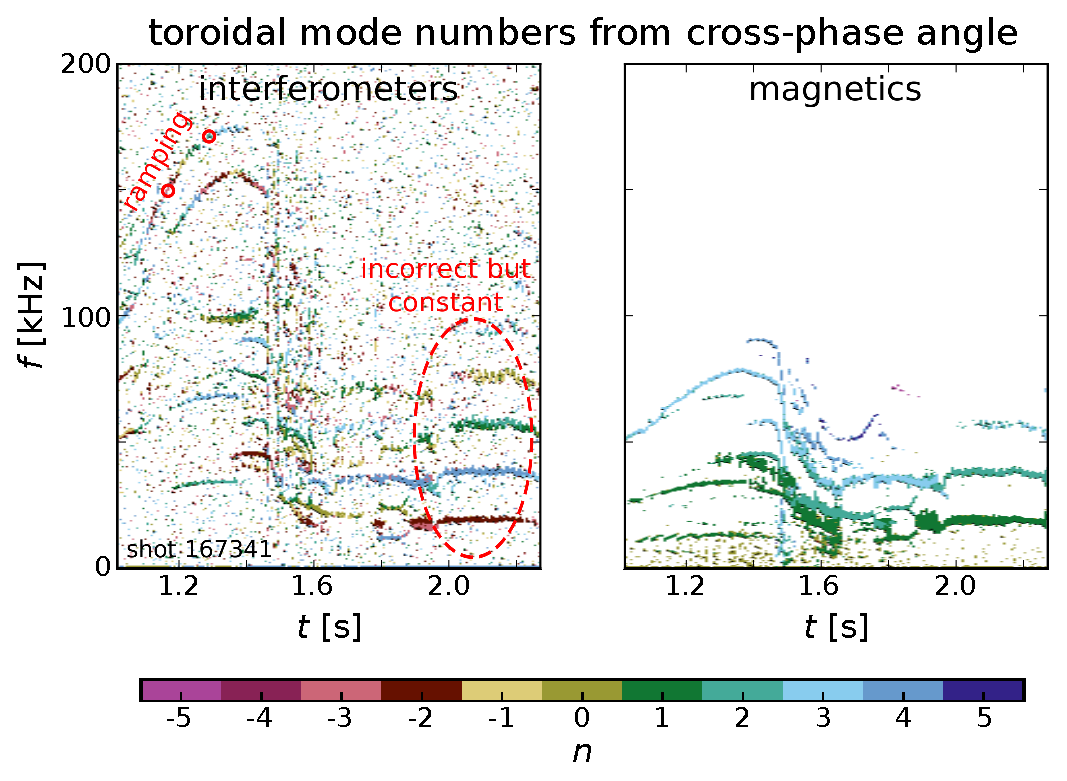
\includegraphics[width = \textwidth]{%
    Chapters/ToroidalCorrelation/figs/mode_numbers_with_uncompensated_time_delay.eps}
  \caption{Computed mode numbers from
    toroidally separated interferometers and magnetics.
    When there is an uncompensated time delay ($\delta t \neq 0$)
    between the two interferometers, as there is here,
    the interferometer-measured mode numbers
    for both constant-frequency and ramping-frequency modes
    are \emph{incorrectly} computed.}
\label{fig:ToroidalCorrelation:uncompensated_time_delay}
\end{figure}

Now, Fig.~\ref{fig:ToroidalCorrelation:uncompensated_time_delay} shows an example
of the computed toroidal mode number spectrum
when using the native time-bases of the V2 and PCI interferometers;
the corresponding magnetics spectrum is shown for comparison.
For $t \lesssim \SI{1.5}{\second}$
the mode frequencies are ramping approximately linearly in time, and
the interferometer-measured mode number is (artificially) ramping in time,
in contrast to the corresponding measurements from magnetics;
application of
(\ref{eq:ToroidalCorrelation:toroidal_mode_number_dt_ramp_rate_lab_frame})
to the \emph{highest-frequency} mode observed by the interferometers yields
$\delta t \approx \SI{-30}{\micro\second}$
($\Delta n = 5$, $\Delta f \approx \SI{20}{\kilo\hertz}$,
as indicated by the positions of the small circular annotations
to the highest frequency mode in
Fig.~\ref{fig:ToroidalCorrelation:uncompensated_time_delay}).
Further, note that the mode number evolution \emph{reverses}
after the mode reaches its peak frequency,
in agreement with the behavior expected from
(\ref{eq:ToroidalCorrelation:toroidal_mode_number_dt_ramp_rate_lab_frame}).
Finally, for $t \gtrsim \SI{2}{\second}$
the mode frequencies are constant, but
the interferometer-measured mode numbers are in disagreement with magnetics.
Naive application of
(\ref{eq:ToroidalCorrelation:toroidal_mode_number_dt_constant_omega})
to the \emph{lowest-frequency} mode at $f \approx \SI{20}{\kilo\hertz}$
yields $\delta t \approx \SI{20}{\micro\second}$
($n_{\text{meas}} = -2$, $n = 1$,
$\omega \approx 2 \pi \cdot \SI{20}{\kilo\hertz}$),
in contrast with the above time-delay estimate
from the linearly ramping mode numbers.
However, as warned above,
$n_{\text{meas}}$ will be \emph{aliased} for ``large'' time delays:
using the above parameters for the lowest-frequency mode,
we see that $|\omega \delta t / \Delta \zeta| \approx 4.8 > n_{\text{Ny}}$,
where $n_{\text{Ny}} = 4$ is the Nyquist mode number
for the $\Delta \zeta = 45^{\circ}$ toroidal separation of the interferometers,
confirming that aliasing has biased our time-delay estimate.
To account for aliasing, we can take $n_{\text{meas}} = -2 \rightarrow 6$, and
application of
(\ref{eq:ToroidalCorrelation:toroidal_mode_number_dt_constant_omega}) yields
$\delta t \approx -\SI{30}{\micro\second}$,
in agreement with the time-delay estimate
from the linearly ramping mode numbers!

The above observations are all consistent with there being an offset
between the native time-bases of the PCI and V2 interferometers, and
the two \emph{independent} measurements of this time offset are in agreement,
with each yielding an offset $\delta t \approx \SI{-30}{\micro\second}$.
Indeed, delaying the PCI signal by $-\SI{30}{\micro\second}$
relative to the V2 signal in software dramatically improves
the agreement between the interferometer and magnetics mode number spectra.
By scanning $\delta t$ about $-\SI{30}{\micro\second}$ and
noting when discrepancy with magnetics began to creep back into
the interferometer-measured mode spectrum,
the upper and lower bounds of $\delta t$ were found;
the best estimate for $\delta t$ was then taken as the midpoint
between these upper and lower bounds, which was found to be
\begin{equation}
  \delta t = -\SI{32}{\micro\second}
  \label{eq:ToroidalCorrelation:time_delay}
\end{equation}
That is, the native PCI-interferometer's time base \emph{leads}
the native V2 time base by $\SI{32}{\micro\second}$.
Delaying the PCI-interferometer by $\SI{32}{\micro\second}$ (in software)
relative to the V2 interferometer yields the mode number spectrum
shown in Fig.~\ref{fig:ToroidalCorrelation:compensated_time_delay}.
Note that both
Fig.~\ref{fig:ToroidalCorrelation:uncompensated_time_delay} and
Fig.~\ref{fig:ToroidalCorrelation:compensated_time_delay}
correspond to shot 167341, and
the only difference in the interferometer-measured mode number spectrum
between the two figures results from the compensation of the time delay
between the native time bases of the two interferometers.

\textcolor{red}{Note that additional measurements are needed
to determine which clock is correct in the \emph{absolute} sense.
For example, we can try digitizing a trigger signal and
comparing the digitized time of the trigger to the ``nominal'' trigger time
to determine the offset of our digitizer from the DIII-D clock.}

\begin{figure}
  \centering
  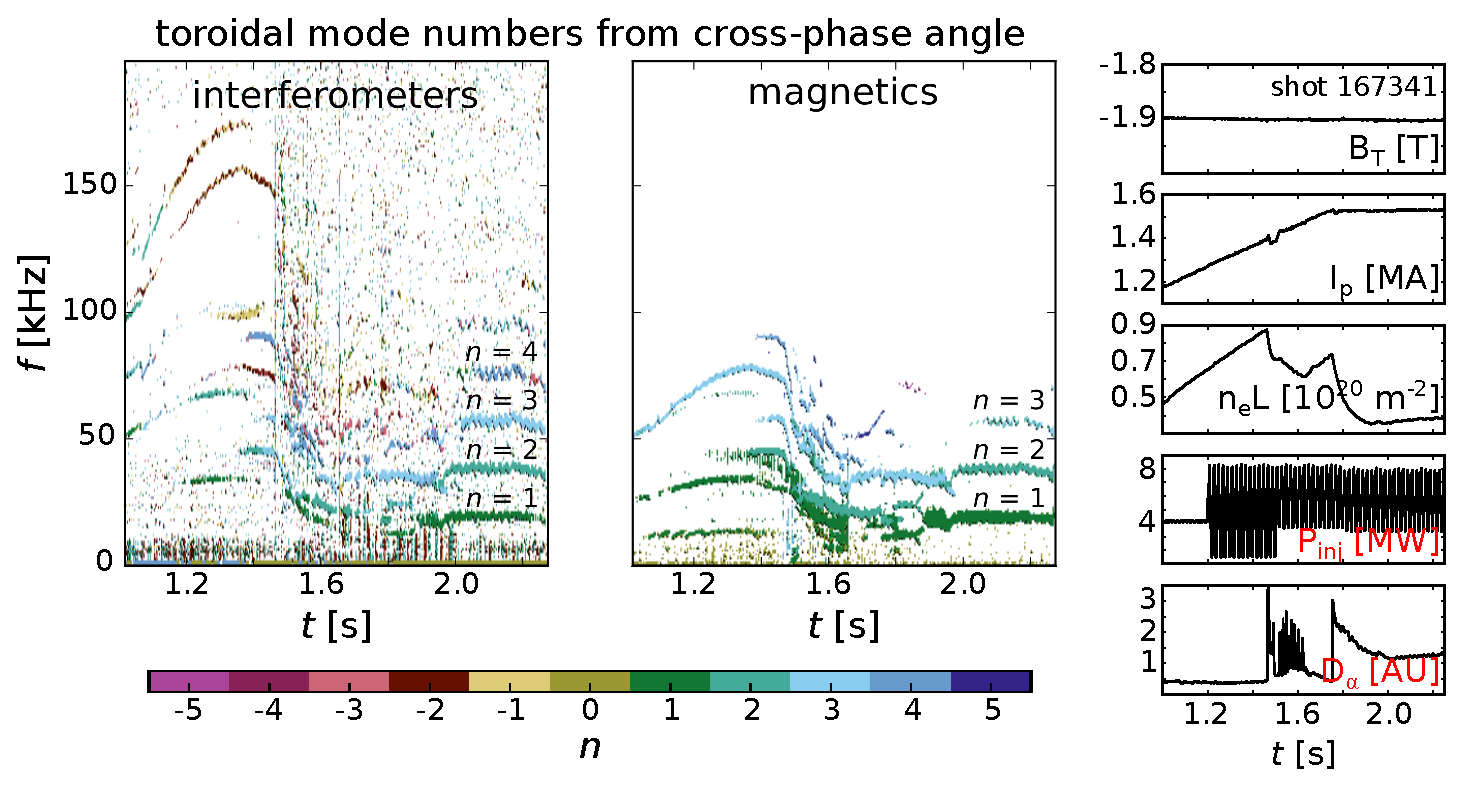
\includegraphics[width = \textwidth]{%
    Chapters/ToroidalCorrelation/figs/magnetics_and_interferometer_mode_numbers_167341.eps}
  \caption{Computed mode numbers from
    toroidally separated interferometers and magnetics.
    Here, the PCI-interferometer signal has been delayed by
    $\SI{32}{\micro\second}$ relative to the V2 signal
    to account for the time offset between each system's native time base.
    Note that the agreement with magnetics is excellent and that
    the mode numbers of the ramping-frequency modes are no longer
    artificially ramping;
    this is an enormous improvement over the corresponding
    uncompensated interferometer-measured spectrum in
    Fig.~\ref{fig:ToroidalCorrelation:uncompensated_time_delay}.}
\label{fig:ToroidalCorrelation:compensated_time_delay}
\end{figure}


\subsection{Radial offset}
The V2 and PCI interferometer beam paths have a slight radial offset
($\Delta R = \SI{4}{\centi\meter}$ with
$R_{\text{V2}} = \SI{1.94}{\meter}$ and $R_{\text{PCI}} = \SI{1.98}{\meter}$).
Thus, $\alpha_{12} = n(\zeta_2 - \zeta_1) + [\sigma(R_2) - \sigma(R_1)]$.
Recall that $\sigma_F$ is a complicated function of
the beam's major radial location,
the mode structure,
the equilibrium density profile, and
the plasma geometry.
However, the \emph{dominant} effect of such a radial offset
is attributable to the relative phase of $\vect{\xi}$
at the two radial locations:
\begin{equation}
  \sigma(R_2) - \sigma(R_1)
  \approx
  \begin{cases}
    0, & \quad \text{$\vect{\xi}(R_1)$ and $\vect{\xi}(R_2)$ in-phase} \\
    \pi, & \quad \text{$\vect{\xi}(R_1)$ and $\vect{\xi}(R_2)$ out-of-phase}
  \end{cases}
  \notag
\end{equation}
If $\vect{\xi}(R_1)$ and $\vect{\xi}(R_2)$ are in-phase,
then application of (\ref{eq:ToroidalCorrelation:toroidal_mode_number_ideal})
will yield the correct mode number.
However, if $\vect{\xi}(R_1)$ and $\vect{\xi}(R_2)$ are out-of-phase,
then application of (\ref{eq:ToroidalCorrelation:toroidal_mode_number_ideal})
will yield a measured mode number $n_{\text{meas}}$
\begin{equation}
  n_{\text{meas}}
  =
  \begin{cases}
    n + n_{\text{Ny}}, & \quad n \leq 0 \\
    n - n_{\text{Ny}}, & \quad n > 0
  \end{cases}
  \label{eq:ToroidalCorrelation:toroidal_mode_number_radially_out_of_phase}
\end{equation}
where $n_{\text{Ny}} \equiv \pi / \Delta \zeta$
is the Nyquist toroidal mode number, and
the $n > 0$ case results from \emph{aliasing}
(that is, $n + n_{\text{Ny}} \rightarrow n - n_{\text{Ny}}$
when $n > 0$ because of aliasing).
Lacking additional measurements or some type of forward modeling,
this incorrect mode-number identification may go undiagnosed.
However, if $\vect{\xi}(R)$ evolves such that
$\vect{\xi}(R_1)$ and $\vect{\xi}(R_2)$ transition
from being in-phase to being out-of-phase (or vice versa),
the measured mode number will ``flip'';
an example of this mode-number ``flipping''
is shown in Fig.~\ref{fig:ToroidalCorrelation:mode_number_flips}.
Further effects of the radial offset can be investigated
via e.g.\ forward modeling and synthetic diagnostics.

\begin{figure}
  \centering
  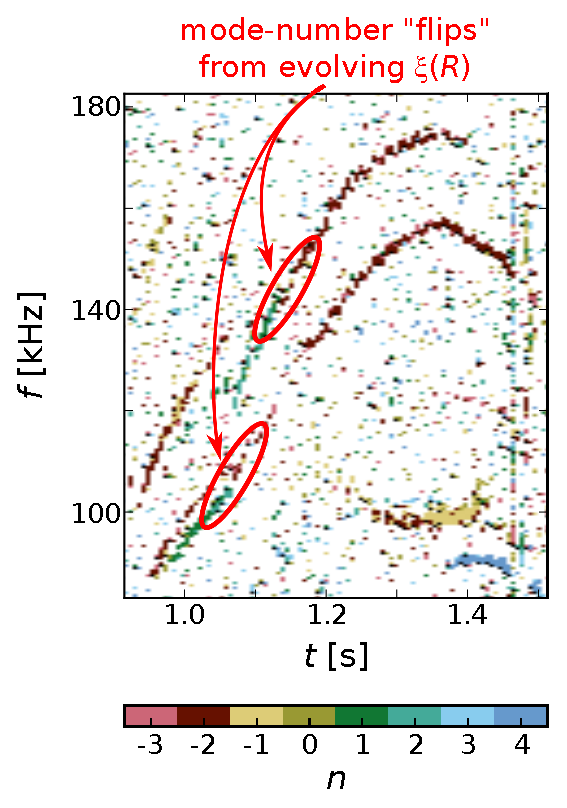
\includegraphics[width = 0.5 \textwidth]{%
    Chapters/ToroidalCorrelation/figs/phase_flips_167341.eps}
  \caption{Due to the small radial offset ($\Delta R = \SI{4}{\centi\meter}$)
    between the V2 and PCI interferometers,
    changes in the radial structure of a mode
    can result in ``flipping'' of the interferometer-measured mode number.
    Here, the mode number flips from $n = 2$ to $n = -2$,
    consistent with
    (\ref{eq:ToroidalCorrelation:toroidal_mode_number_radially_out_of_phase}).
    Lacking additional measurements or some type of forward modeling,
    it is impossible to determine if the mode is truly $n = 2$ or $n = -2$.
    Note that these modes exceed the typical bandwidth of magnetics, however,
    so even identification as $n = \pm 2$ \emph{is} an improvement!}
\label{fig:ToroidalCorrelation:mode_number_flips}
\end{figure}


\section{Example mode number spectra}

\begin{figure}[h!]
  \centering
  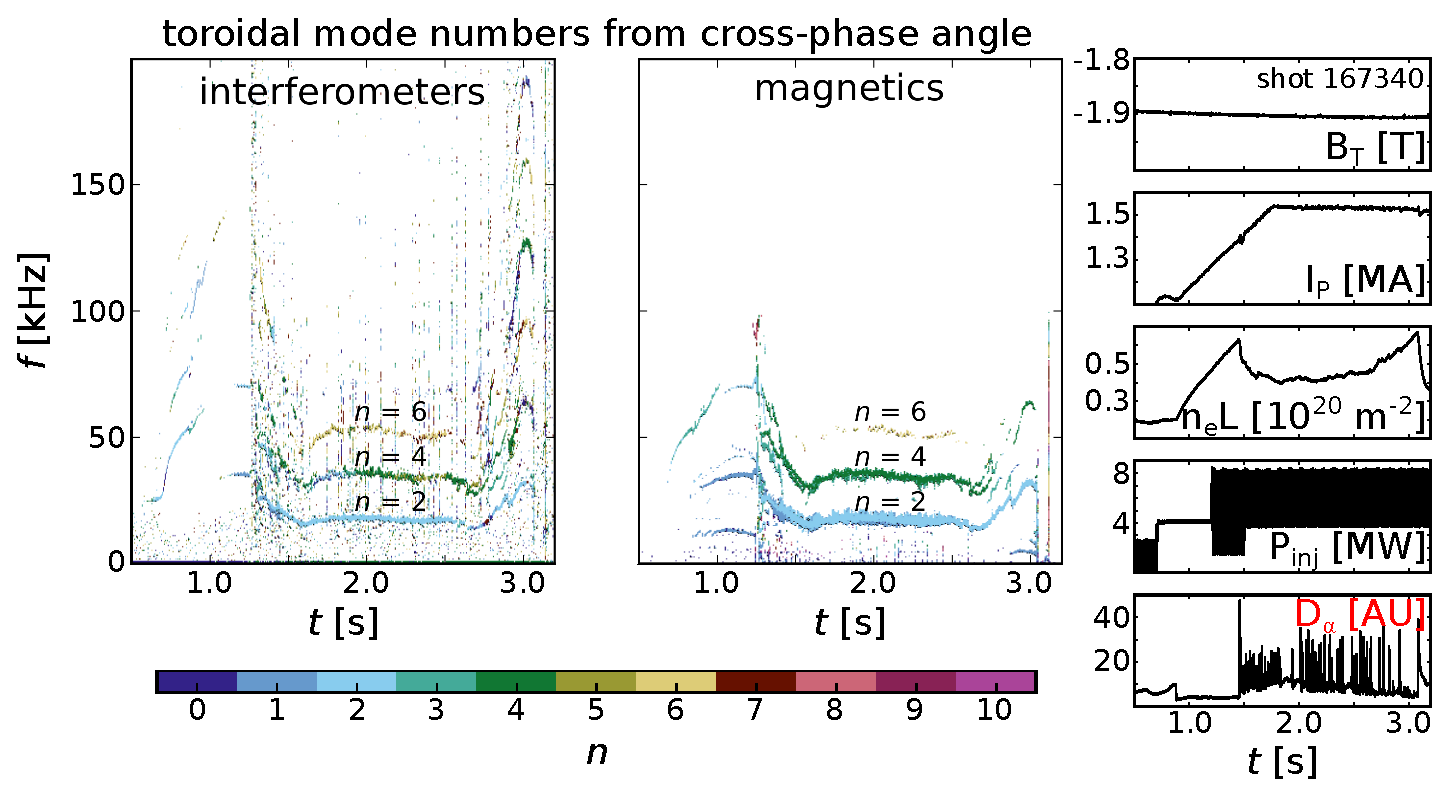
\includegraphics[width = \textwidth]{%
    Chapters/ToroidalCorrelation/figs/magnetics_and_interferometer_mode_numbers_167340.eps}
  \caption{Another example of excellent agreement between the
    interferometer and magnetics mode number spectra. Note that
    the interferometers additionally see modes \emph{invisible} to magnetics.
    Here,the modes were \emph{assumed} to be rotating
    in the ``positive'' direction
    (i.e.\ counterclockwise when viewing the torus from above,
    as this corresponds to the direction of dominant torque injection)
    such that we can discriminate $0 \leq n < 8$
    (rather than the typical $-4 < n \leq 4$).}
\label{fig:ToroidalCorrelation:magnetics_corroboration_2}
\end{figure}

\begin{figure}[h!]
  \centering
  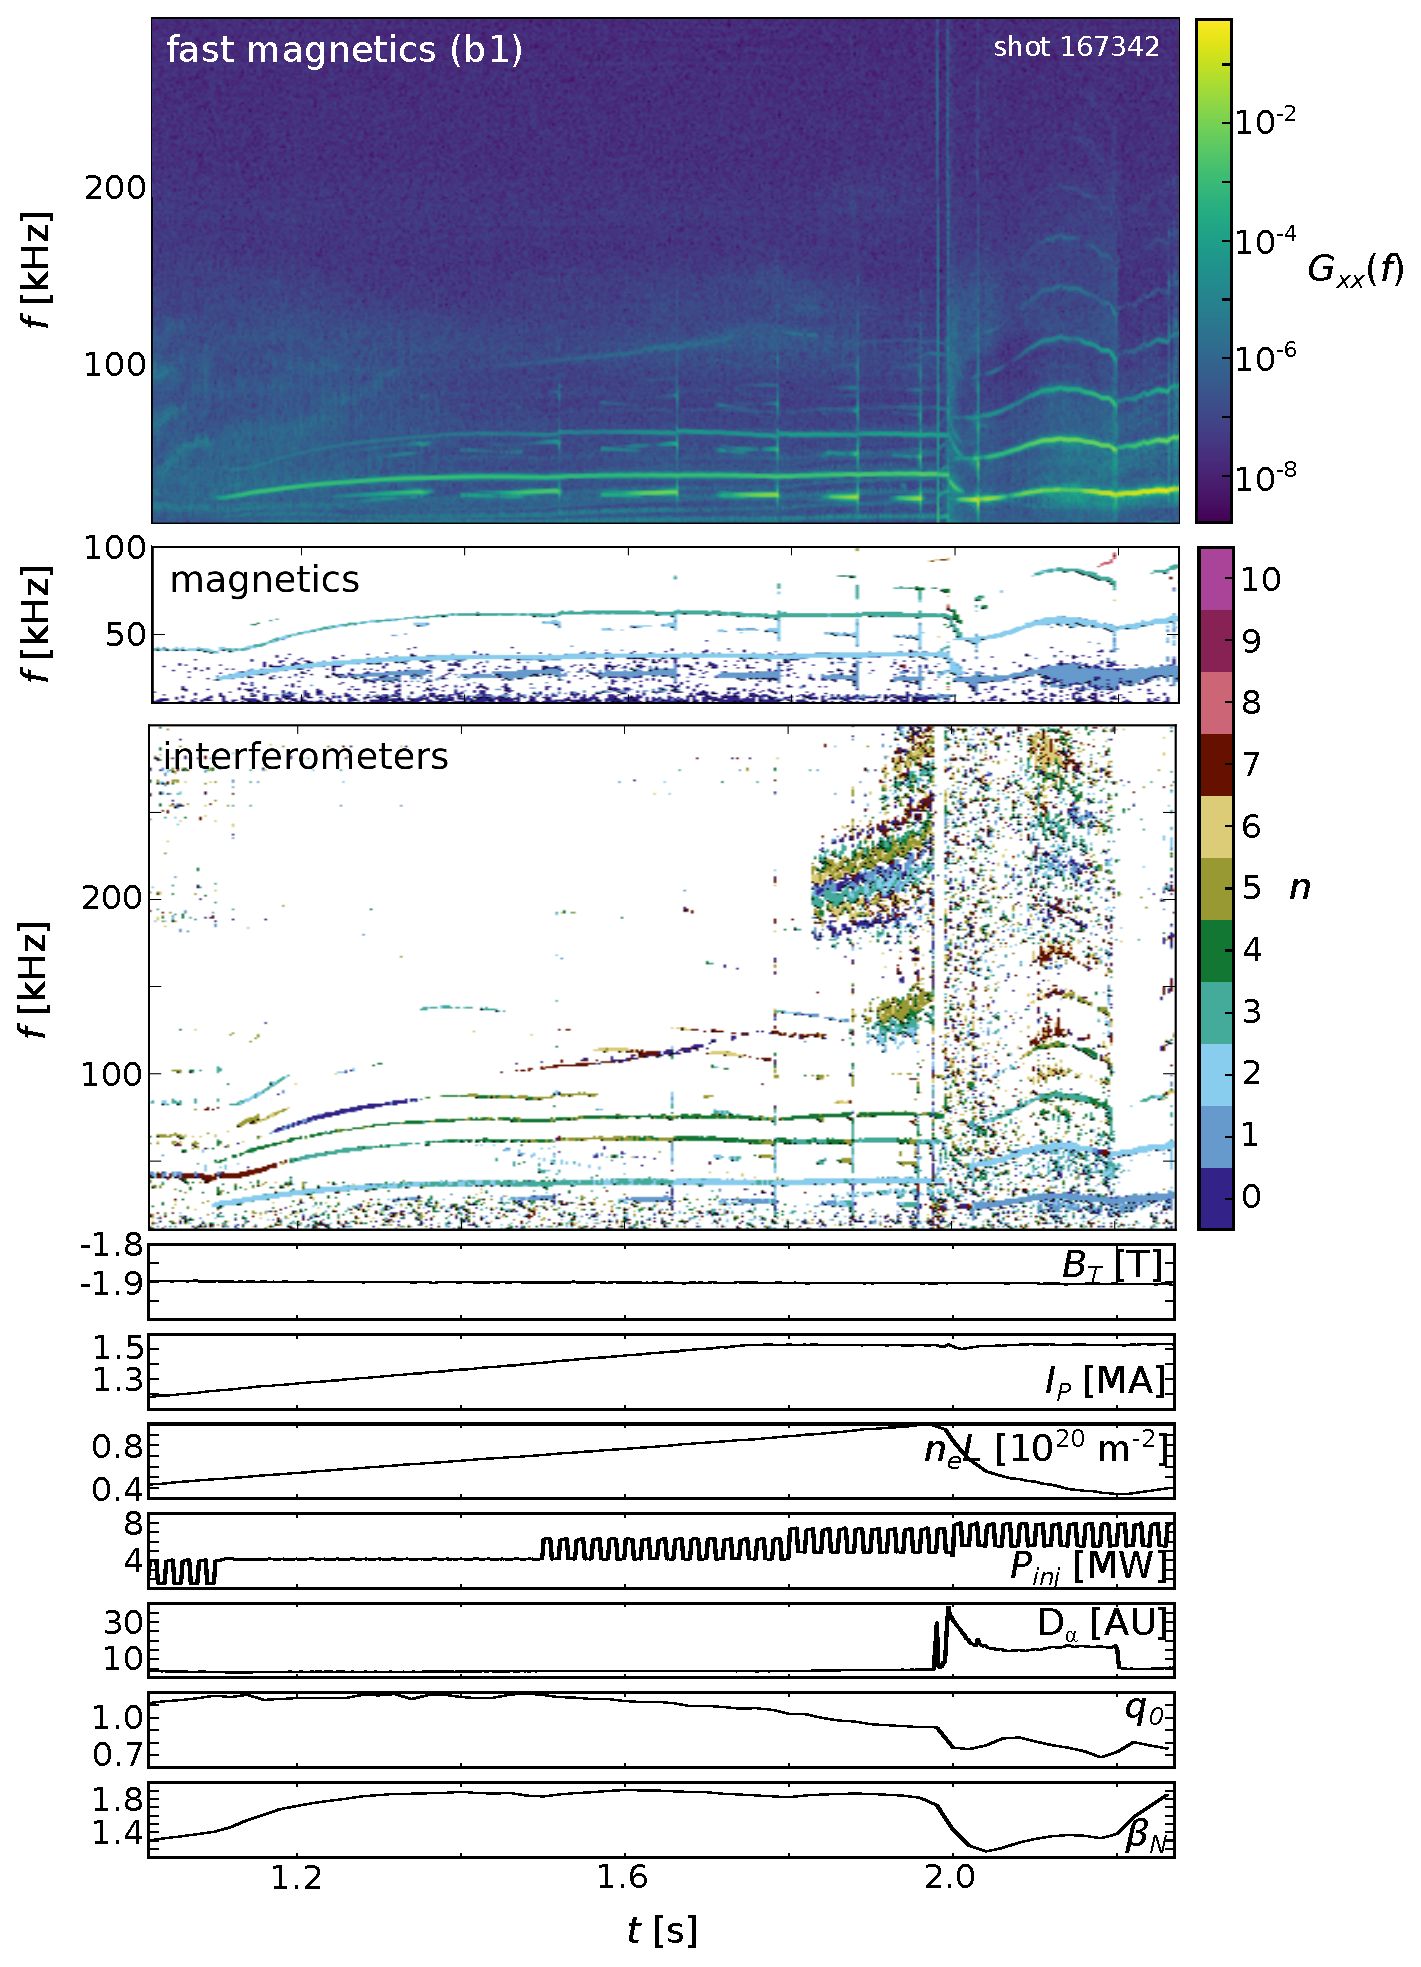
\includegraphics[width = 0.8 \textwidth]{%
    Chapters/ToroidalCorrelation/figs/core_localized_167342.eps}
  \caption{Between $1.8 \leq t \, [\text{s}] \leq 2.2$,
    the correlated interferometers measure fluctuations
    (Alfv\'{e}n eigenmodes?) that are \emph{invisible} to magnetics.
    This suggests that the modes are \emph{core-localized} and
    that the correlated interferometers are indeed capable
    of measuring core-localized MHD!
    (Note that the fast magnetic probes have a \SI{1}{\mega\hertz} bandwidth,
    but they do not have significant toroidal separation,
    preventing accurate measurement of toroidal mode numbers).}
\label{fig:ToroidalCorrelation:core_localized}
\end{figure}

\begin{figure}[h!]
  \centering
  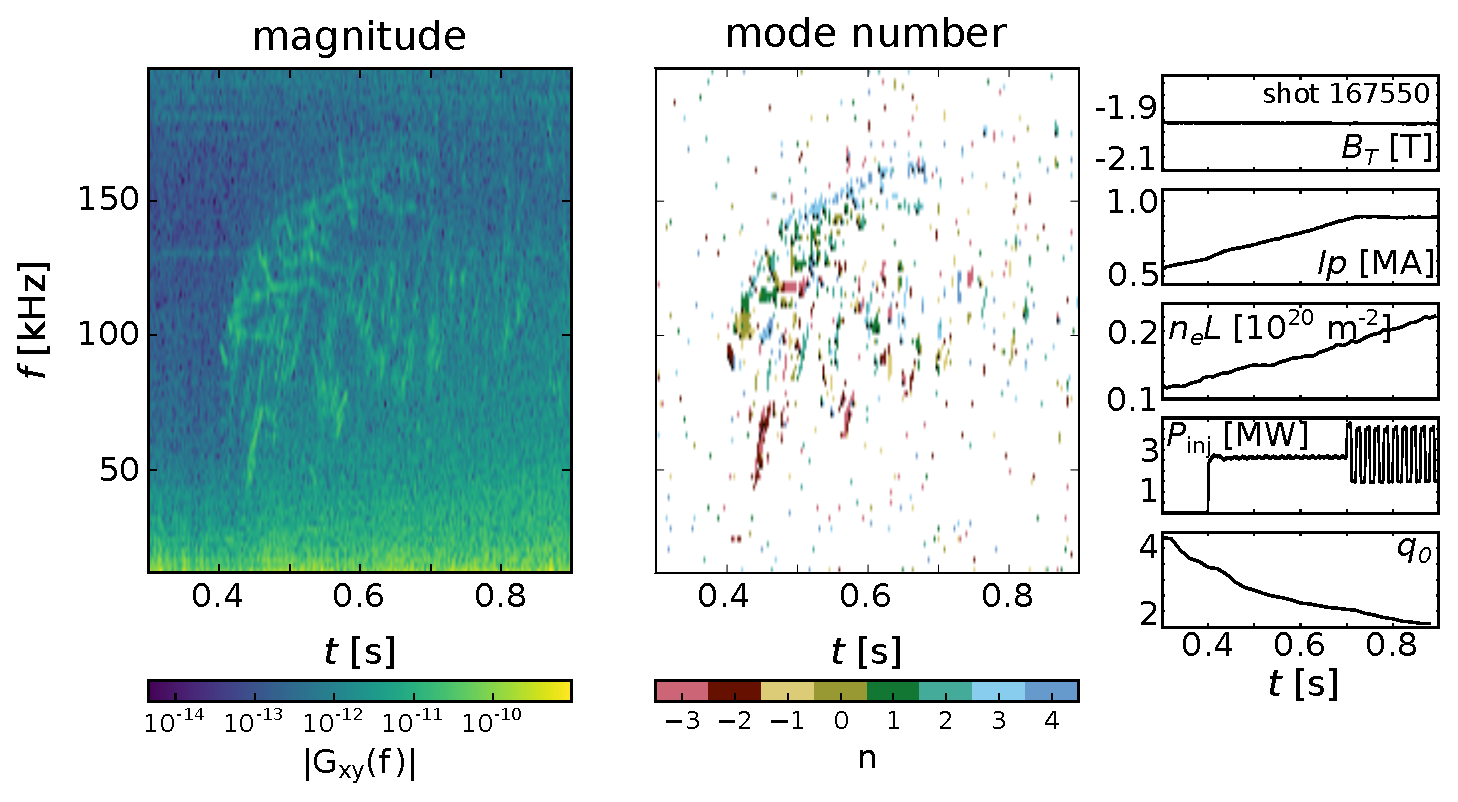
\includegraphics[width = \textwidth]{%
    Chapters/ToroidalCorrelation/figs/AEs_167550.eps}
  \caption{Alfv\'{e}n eigenmodes (?) visible
    on the correlated interferometers.
    These modes are not readily visible on magnetics.}
\label{fig:ToroidalCorrelation:AEs}
\end{figure}

\begin{figure}[h!]
  \centering
  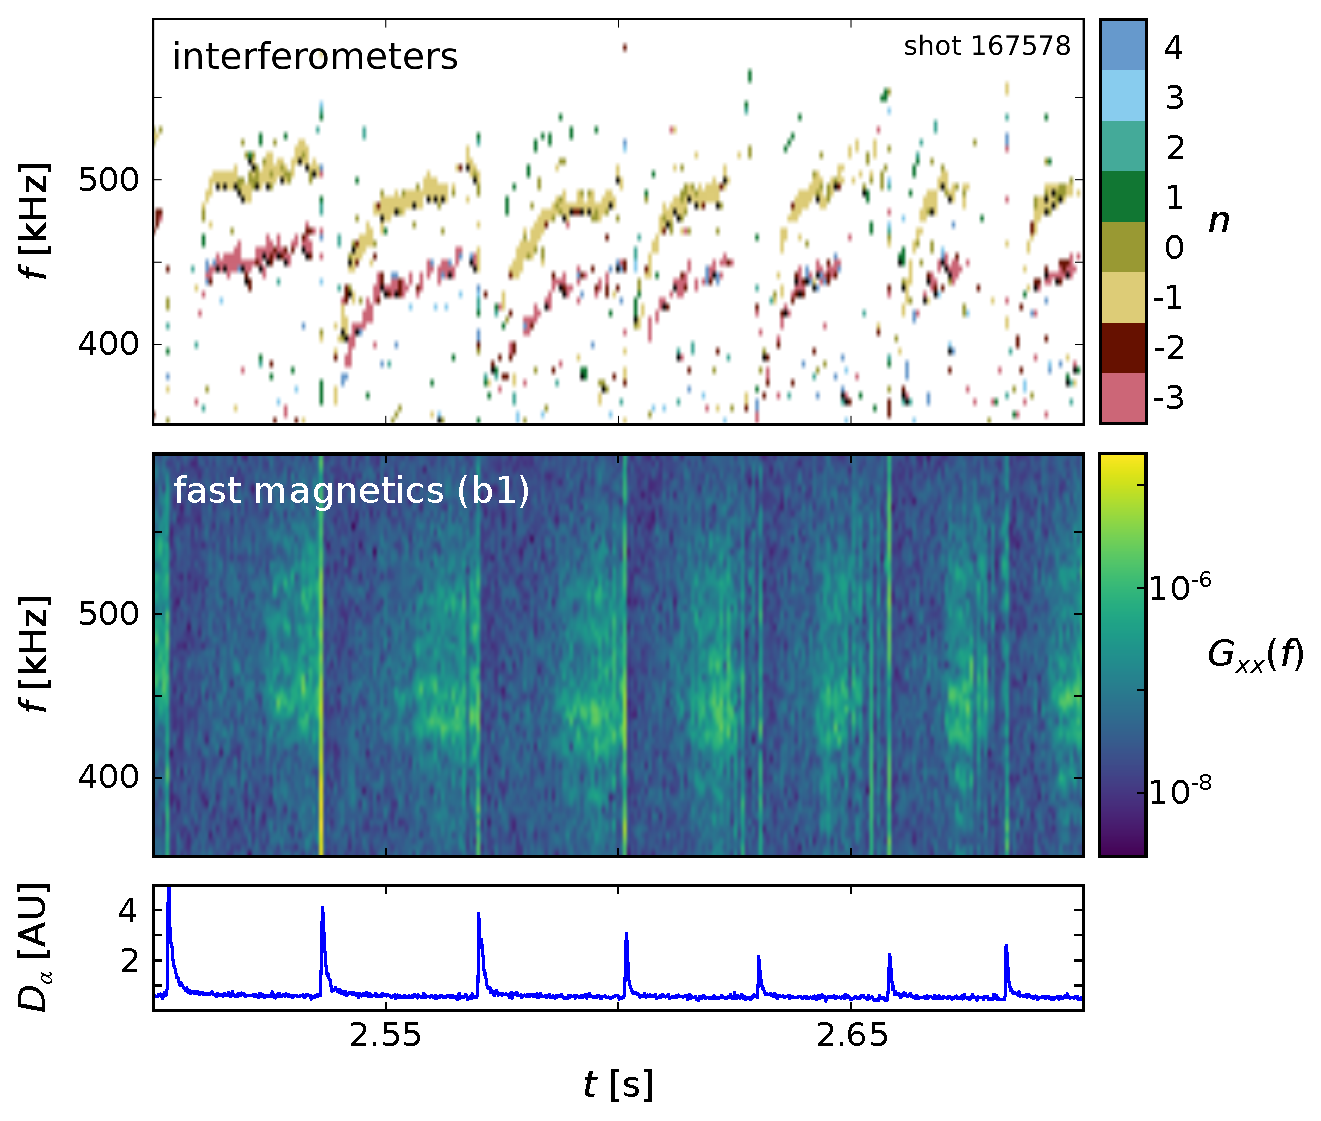
\includegraphics[width = 0.7 \textwidth]{%
    Chapters/ToroidalCorrelation/figs/interELM_fast_167578.eps}
  \caption{Inter-ELM fluctuations as measured by
    the correlated interferometers and fast magnetics.
    The mode frequency ramps early in the inter-ELM window before saturating;
    the magnetic component of the fluctuation only appears \emph{after}
    the mode frequency has saturated --- fascinating!
    (Note that the fast magnetic probes have a \SI{1}{\mega\hertz} bandwidth,
    but they do not have significant toroidal separation,
    preventing accurate measurement of toroidal mode numbers).
    The drive and significance of such fluctuations is not known, but
    they do \emph{not} occur in every ELMy discharge.}
\label{fig:ToroidalCorrelation:interELM_fast}
\end{figure}

\begin{figure}[h!]
  \centering
  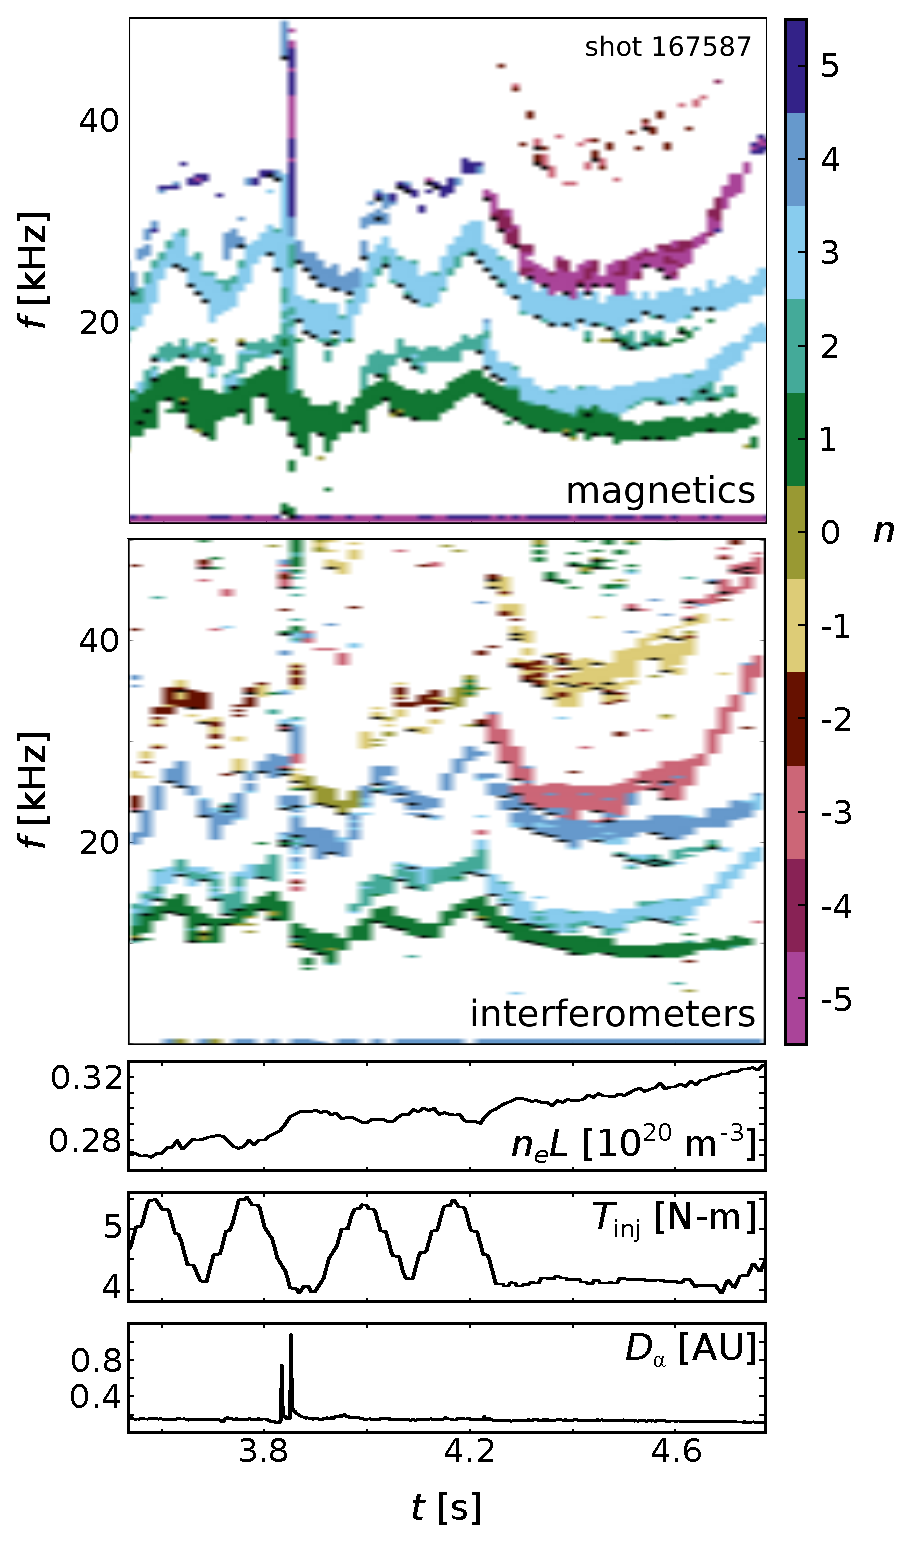
\includegraphics[width = 0.5 \textwidth]{%
    Chapters/ToroidalCorrelation/figs/EHO_167587.eps}
  \caption{The magnetics and interferometers both see the
    edge harmonic oscillation (EHO), which is responsible for
    flushing impurities from quiescent H-mode (QH-mode) plasmas.
    Below \SI{20}{\kilo\hertz}, the magnetics and interferometers
    both measure the same toroidal mode numbers; however,
    above \SI{20}{\kilo\hertz}, the measured mode numbers differ,
    likely due to a combination of aliasing and the small radial offset
    of the two interferometer beams.}
\label{fig:ToroidalCorrelation:EHO}
\end{figure}

\begin{figure}[h!]
  \centering
  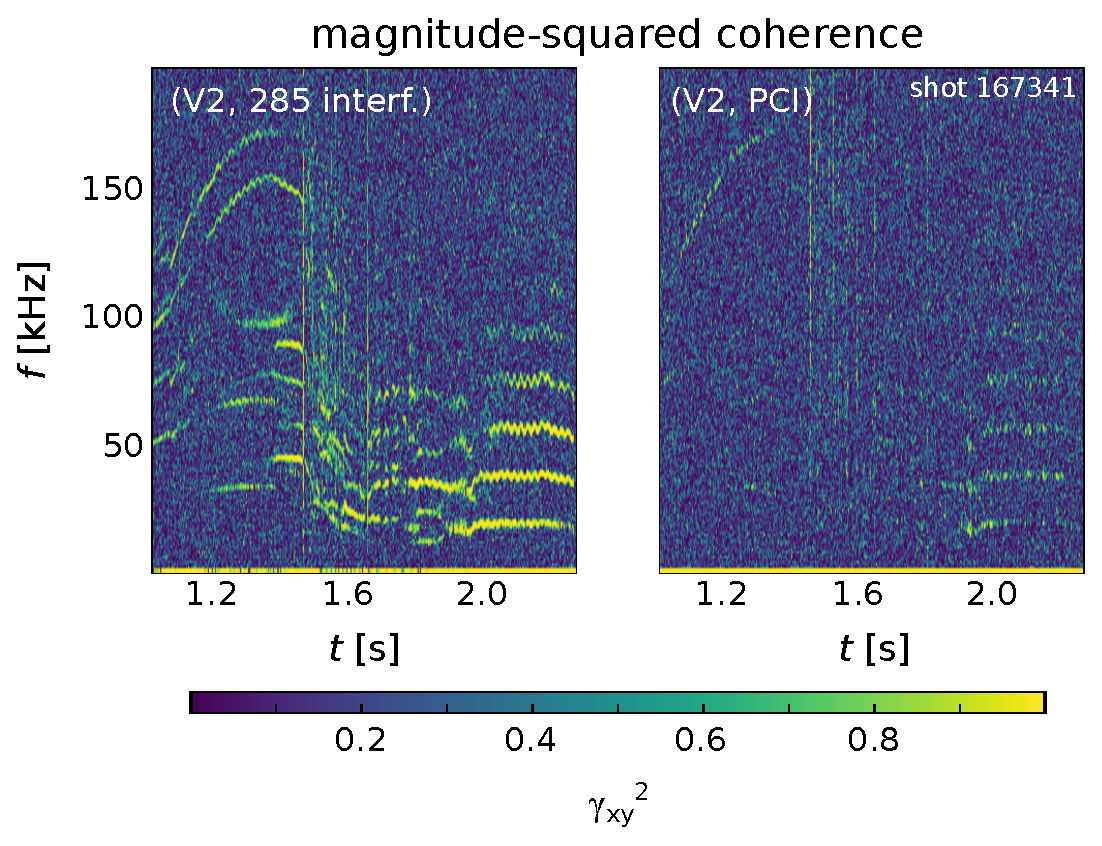
\includegraphics[width = 0.75 \textwidth]{%
    Chapters/ToroidalCorrelation/figs/interferometer_vs_PCI_coherence.eps}
  \caption[%
    Inability to correlate V2 and PCI]{%
      The magnitude-squared coherence $\gamma_{xy}^2$ between
      the V2 and 285 interferometers (left) and
      between the V2 interferometer and PCI (right).
      The high coherence between the V2 and 285 interferometers
      allows accurate measurement of toroidal mode numbers,
      as demonstrated by the corresponding mode number spectrum
      displayed in Fig.~\ref{fig:ToroidalCorrelation:compensated_time_delay},
      whereas the poor coherence between the V2 and PCI
      prevents such measurements.
      (Note that ``285 interferometer'' refers to
      the newly installed interferometer channel of the PCI).}
\label{fig:ToroidalCorrelation:PCI_coherence}
\end{figure}


\bibliographystyle{plainurl}
\bibliography{references}
%
\chapter{Multiscale turbulence measurements}
\label{ch:TurbulenceMeasurements}
Development of a first-principles understanding
of turbulent transport in a tokamak
requires multi-tiered validation\ldots
comparing not just heat fluxes, but
also turbulent spectra etc.
\diiid's extensive suite of fluctuation diagnostics
provides an ideal setting to validate
predicted changes~\cite{howard_pp16}
to turbulent spectra when altering relative drive
between electron-scale and ion-scale turbulence.


\section{Overview of multiscale gyrokinetic predictions}


\section{Experimental conditions}
The experiment was run in the ITER-similar shape,
with aspect ratio, elongation, and triangularity
all closely matched to those of the ITER-baseline scenario
\cite[Sec.~13.5 \& 13.6]{wesson}.
The on-axis toroidal field $B_T = \SI{1.7}{\tesla}$ and
plasma current $I_p = \SI{1.3}{\mega\ampere}$
produced $q_{95} = 3.15$,
where $q_{95}$ is the average value
of the safety factor $q$~\cite[Sec.~3.4]{wesson}
over the surface that encloses $95\%$
of the poloidal flux within the last-closed flux surface.
The neutral beams~\cite[Sec.~5.3-5.5]{wesson}
were operated with feedback to maintain
$\beta_N = 1.9$, where
$\beta_N$ is the normalized plasma pressure~\cite[Sec.~6.18]{wesson}.
In order to suppress core MHD,
an average neutral-beam torque of $\sim \SI{1.5}{\newton \meter}$
was injected into the plasma;
note that this is $\sim 4\times$ larger than
the projected ITER-equivalent torque~\cite{garofalo_nf11}.
In order to alter the local electron-scale and ion-scale drives,
the electron cyclotron resonance heating (ECH)~\cite[Sec.~5.10]{wesson}
location was scanned between $\rho = 0.5$ and $\rho = 0.8$,
where $\rho$ is the square root of the normalized toroidal flux
(which scales as $r / a$, with
$r$ being the minor-radial coordinate and
$a$ being the minor radius of the plasma).
Intra-shot scans of the ECH location
were plagued with core MHD, so
only shot-to-shot, MHD-free scans of the ECH location
are considered here.
The line-averaged density was
$\bar{n}_e = \SI{5.2e19}{\per\meter\cubed}$.
Impurities are removed from the plasma
by both large and small edge localized modes (ELMs)~\cite[Sec.~7.17]{wesson}.
The time histories of several actuators and plasma parameters
are shown in Figure~\ref{fig:TurbulenceMeasurements:traces}.
Note that multiscale gyrokinetic simulations
of this experiment's reference discharge,
\diiid\space shot $153523$ with ECH at $\rho = 0.5$,
indicate that the turbulent transport
is intrinsically multiscale in nature~\cite{holland_nf17}.

\begin{figure}
  \centering
  \includegraphics[width = \textwidth]{%
    Chapters/TurbulenceMeasurements/figs/traces.png}
  \caption[Time histories of various actuators \& plasma parameters]{%
    Time histories of various actuators and plasma parameters:
    (a) plasma current $I_p$,
    (b) neutral beam injected (NBI) power $P_{\text{inj}}$,
    (c) NBI torque $T_{\text{inj}}$,
    (d) electron cyclotron resonance heating (ECH) power $P_{\text{ECH}}$,
    (e) line-averaged density $\bar{n}_e$,
    (f) normalized plasma pressure $\beta_N$,
    (g) confinement quality $H_{98,\text{y}2}$, and
    (h) divertor $D_{\alpha}$ light, indicating
    the presence of large and small edge localized modes (ELMs).
    The ECH heating location was
    at $\rho = 0.5$ in $171536$ and
    at $\rho = 0.8$ in $171538$.
  }
\label{fig:TurbulenceMeasurements:traces}
\end{figure}

Equilibrium profiles
\begin{itemize}
  \item averaging over \textcolor{red}{XXX ms}
  \item What types of fits? (splines, RBF, etc.)
  \item Electron-density profiles -- Thomson w/ CO$_2$ normalization?
    Reflectometer?
  \item Electron-temperature profiles -- Thomson \& ECE (or ECE cutoff?)
  \item Ion-temperature profiles -- \textcolor{red}{???}
  \item CER provides C$^{6+}$ density, temperature, and rotation
  \item $E_r$ computed using force balance for
    C$^{6+}$ pressure and toroidal rotation.
    \textcolor{red}{poloidal rotation neglected?}
  \item \textcolor{red}{MSE-constrained EFIT? Kinetic?}
  \item \textcolor{red}{How are ELMs handled?}
  \item Uncertainties
  \item Clear change in turbulent drives with ECH location
\end{itemize}

\begin{figure}
  \centering
  \includegraphics[width = \textwidth]{%
    Chapters/TurbulenceMeasurements/figs/profiles.pdf}
  \caption[Profiles \& inverse scale lengths]{%
    Profiles \& inverse scale lengths from
    OMFIT['TGLF\_scan']['tgyro\_output']
    used as input for TGLF simulations.
  }
\label{fig:TurbulenceMeasurements:profiles}
\end{figure}

\begin{figure}
  \centering
  \includegraphics[width = \textwidth]{%
    Chapters/TurbulenceMeasurements/figs/Er_profiles.pdf}
  \caption[Radial electric field \& $E \times B$ shearing rate]{%
    Radial electric field \& $E \times B$ shearing rate from
    OMFIT['TGLF\_scan']['TGYRO']['PROFILES\_GEN']['OUTPUTS']['Er']
    (note that there are no corresponding values from
    OMFIT['TGLF\_scan']['tgyro\_output']
    from which Figure~\ref{fig:TurbulenceMeasurements:profiles}
    was generated, which is why this is a separate figure\ldots).
  }
\label{fig:TurbulenceMeasurements:Er_profiles}
\end{figure}


\section{Measurements}
\begin{figure}[h!]
  \centering
  \includegraphics[width = 0.9 \textwidth]{%
    Chapters/TurbulenceMeasurements/figs/spectra_171521_quarterly_review.pdf}
  \caption[Combined PCI-interferometer measured spectra]{%
    Combined PCI-interferometer measured spectra.
  }
\label{fig:TurbulenceMeasurements:spectra_quarterly_review}
\end{figure}

\begin{figure}[h!]
  \centering
  \includegraphics[width = \textwidth]{%
    Chapters/TurbulenceMeasurements/figs/Skf_annotated.png}
  \caption[PCI-measured $S(k, f)$ with branch annotations]{%
    PCI-measured $S(k, f)$ with branch annotations.
  }
\label{fig:TurbulenceMeasurements:Skf_annotated}
\end{figure}

\begin{figure}[h!]
  \centering
  \includegraphics[width = 0.6 \textwidth]{%
    Chapters/TurbulenceMeasurements/figs/Sk_power_law.pdf}
  \caption[PCI-measured power law]{%
    PCI-measured power law from branches annotated in
    Figure~\ref{fig:TurbulenceMeasurements:Skf_annotated}.
  }
\label{fig:TurbulenceMeasurements:Sk_power_law}
\end{figure}


\section{TGLF modeling}
\begin{figure}[h!]
  \centering
  \includegraphics[width = \textwidth]{%
    Chapters/TurbulenceMeasurements/figs/doppler_shift.pdf}
  \caption[Doppler shift]{%
    Doppler shift. Positive \& negative values of $v_{\text{pci}}$
    correspond to above \& below the midplane, respectively.
    As the mask was not used, we cannot determine whether or not
    $v_{\text{meas}}$ corresponds to above or below the midplane, however
    (hence we plot $\pm v_{\text{meas}}$).
  }
\label{fig:TurbulenceMeasurements:doppler_shift}
\end{figure}

\begin{figure}[h!]
  \centering
  \includegraphics[width = \textwidth]{%
    Chapters/TurbulenceMeasurements/figs/TGLF_171536_vs_171538.png}
  \caption[Qualitative presentation of TGLF results]{%
    Qualitative presentation of TGLF results.
  }
\label{fig:TurbulenceMeasurements:TGLF_171536_vs_171538}
\end{figure}

\begin{figure}[h!]
  \centering
  \includegraphics[width = \textwidth]{%
    Chapters/TurbulenceMeasurements/figs/linear_stability.pdf}
  \caption[Growth rates \& frequencies at $\rho=0.7$]{%
    Growth rates \& frequencies at $\rho=0.7$
    (i.e.\ we're slicing
    Figure~\ref{fig:TurbulenceMeasurements:TGLF_171536_vs_171538}
    at $\rho = 0.7$ for the most unstable mode, mode $1$).
    Note that only $171536$ uses SAT\_RULE $= 1$,
    which is calibrated against multiscale GYRO results;
    $171538$ uses SAT\_RULE $= 0$.
    Thus, it is difficult to draw conclusions\ldots
  }
\label{fig:TurbulenceMeasurements:linear_stability}
\end{figure}

\begin{figure}[h!]
  \centering
  \includegraphics[width = \textwidth]{%
    Chapters/TurbulenceMeasurements/figs/density_spectra.pdf}
  \caption[TGLF-predicted density-fluctuation spectra at $\rho=0.7$]{%
    TGLF-predicted density-fluctuation spectra at $\rho=0.7$.
    Note that only $171536$ uses SAT\_RULE $= 1$,
    which is calibrated against multiscale GYRO results;
    $171538$ uses SAT\_RULE $= 0$.
    Thus, it is difficult to draw conclusions\ldots
  }
\label{fig:TurbulenceMeasurements:density_spectra}
\end{figure}


\bibliographystyle{plainurl}
\bibliography{references}
%
\chapter{Conclusions \& future work}
\label{ch:Conclusions}


\section{Summary \& conclusions}
\label{sec:Conclusions:summary_and_conclusions}
The work described in this thesis can be summarized as follows:
\begin{itemize}
  \item Chapter~\ref{ch:InterferometricMethods} discusses
    the theory of optical interferometric methods
    in the context of measuring tokamak plasma-density fluctuations.
    The laser-plasma interaction is quantified via
    Fraunhofer scalar-diffraction theory, and
    the resulting diffracted field is imaged onto a square-law detector.
    Interfering the imaged field with a known reference field
    produces measurable intensity fluctuations;
    the specification of this reference field
    defines the interferometric method.
    Details of two particular interferometric methods ---
    external-reference-beam interferometry and
    phase contrast imaging (PCI) ---
    are discussed, with an emphasis on
    their sensitivity to fluctuations and their spatiotemporal bandwidths.
    Significantly, while PCI can measure fluctuations more sensitively
    than an external-reference-beam interferometer,
    PCI suffers from a low-$k$ cutoff;
    an external-reference-beam interferometer
    does \emph{not} suffer from such a low-$k$ cutoff.
  \item Chapter~\ref{ch:DesignConsiderations} considers the design of an
    external-reference-beam, heterodyne interferometer
    (hereafter referred to as a heterodyne interferometer).
    A criterion for satisfactory wavefront matching
    between the probe beam and the reference beam is developed, and
    finite-sampling-volume effects are shown
    to constrain the heterodyne interferometer's spatial bandwidth.
    The effects of phase noise, amplitude noise, and digitizer bit noise
    are each discussed in the context of
    the heterodyne interferometer's signal-to-noise ratio, and
    the systematic errors resulting from
    imperfect demodulation of the heterodyne interference signal
    are quantified.
  \item Chapter~\ref{ch:Implementation} details
    the addition of a heterodyne interferometer
    to the pre-existing PCI system on the \diiid\space tokamak.
    Both systems operate simultaneously,
    sharing a single $\SI{10.6}{\micro\meter}$ probe beam through the plasma.
    Optical-diagnostic access on \diiid\space and the capabilities
    of the pre-existing PCI system are briefly reviewed.
    Referencing the design considerations
    in Chapter~\ref{ch:DesignConsiderations} and
    adopting the philosophy
    that the pre-existing PCI system should be minimally perturbed,
    the optical layout for the heterodyne interferometer is developed;
    the magnification of the interferometer's imaging system
    is selected such that the spatial bandwidths
    of the PCI and interferometer have a mid-$k$ overlap.
    The design, procurement, and installation
    of the new optical and electrical components
    required to make the heterodyne interferometric measurement
    are summarized.
    Of note is the interferometer's radio-frequency local oscillator:
    the phase noise of a crystal oscillator (XO)
    was empirically found to be \emph{too large}
    to make meaningful fluctuation measurements in most tokamak plasmas, but
    the substantially lower phase noise of an
    oven-controlled crystal oscillator (OCXO)
    allows measurements of a whole zoo
    of coherent and broadband plasma fluctuations.
    The interferometer response and
    the multiscale capabilities of the combined PCI-interferometer
    are empirically verified via sound-wave calibrations.
    Specifically, the PCI is shown to measure high-$k$
    ($\SI{1.5}{\per\centi\meter} < |k_R| \leq \SI{25}{\per\centi\meter}$)
    fluctuations with
    sensitivity $3 \times 10^{13} \; \text{m}^{-2} / \sqrt{\text{kHz}}$,
    while the interferometer simultaneously measures low-$k$
    ($|k_R| < \SI{5}{\per\centi\meter}$) fluctuations with
    sensitivity $3 \times 10^{14} \; \text{m}^{-2} / \sqrt{\text{kHz}}$.
    Both systems have temporal bandwidths in excess of $\SI{1}{\mega\hertz}$.
  \item Chapter~\ref{ch:TurbulenceMeasurements} demonstrates
    the multiscale capabilities of the combined PCI-interferometer.
    During a recent \diiid\space experiment,
    the location of electron cyclotron resonance heating (ECH)
    was moved from $\rhoech = 0.5$ to $\rho_{ECH} = 0.8$,
    altering the local $a / L_{T_e}$ and $a / L_{T_i}$
    in an attempt to change the coupling between
    the electron-scale and ion-scale turbulence.
    As such, this experiment presents an ideal opportunity
    for multiscale turbulence investigations
    with the combined PCI-interferometer.
    Numerous turbulent branches are observed.
    In particular, the interferometer measures
    a low-$k$ electromagnetic mode driven unstable by collisionality,
    properties consistent with the micro-tearing mode (MTM), and
    the PCI measures a wavenumber spectrum
    that exhibits distinct flattening
    when $a / L_{T_e}$ is increased relative to $a / L_{T_i}$,
    reminiscent of results
    from realistic multiscale gyrokinetic simulations~\cite{howard_pp16}.
    To aid the interpretation of these measurements,
    linear-stability analysis and quasilinear-transport modeling
    are performed with the gyro-Landau fluid code TGLF, and
    qualitative agreement with the PCI-measured wavenumber spectrum
    is obtained.
  \item Chapter~\ref{ch:ToroidalCorrelation} discusses the correlation
    of the newly installed interferometer with
    \diiid's toroidally separated, pre-existing $V2$ interferometer.
    Capable of probing the core plasma,
    the interferometers are shown to be sensitive
    to core-localized fluctuations
    that are \emph{invisible} to external magnetic probes.
    The chapter begins with a brief review
    of the two-point correlation technique and
    shows how toroidal mode numbers can be extracted
    from a pair of toroidally separated measurements.
    Meaningful correlation requires that
    the two measurements share the same timebase.
    The digitizers of both interferometers were modified
    to phase lock their clocks, and
    a residual ``trigger offset'' was measured
    and is compensated in software.
    Where comparisons can be made with magnetic probes,
    the interferometer-measured toroidal mode numbers
    are in good agreement.
    Currently, there is not a tested, robust method
    for correcting the bias introduced by
    the $\SI{4}{\centi\meter}$ major-radial offset
    between the interferometer beam centers,
    which unfortunately limits the
    deployment of this system for physics studies
    of core-localized MHD.
\end{itemize}


\section{Future work}
\label{sec:Conclusions:future_work}
The combined PCI-interferometer developed in this work
has a clear application in the burgeoning study
of multiscale turbulence and cross-scale coupling, which
may be significant in the reactor relevant $T_e \approx T_i$ regime.
In roughly the next six months,
Howard \emph{et al.} expects to complete
realistic multiscale gyrokinetic simulations
for the experiment described in
Chapter~\ref{ch:TurbulenceMeasurements}.
It will be very interesting
to see if the predicted wavenumber spectrum
matches the PCI-measured wavenumber spectrum.
It should be noted that a synthetic PCI diagnostic
already exists for the interpretation
of such gyrokinetic simulations~\cite{rost_pp10}.
Small modifications to the synthetic PCI
should also allow a synthetic interferometer diagnostic.
Previous multiscale simulations predict
significant local and non-local energy cascades
between the ion and electron scales~\cite{howard_pp16}, so
it is desirable to investigate such coupling empirically.
With its large spatiotemporal bandwidth,
the combined PCI-interferometer may be ideally suited
for measurement of such coupling, which
may be suitably quantified by
the bicoherence~\cite{young_and_powers_ieee79}
between various channels of the system or
some other suitable measure of nonlinear processes.
(Note that the author has performed preliminary bispectral analysis
of the measurements discussed in
Chapter~\ref{ch:TurbulenceMeasurements};
interestingly, the $|k_R| \sim \SI{5}{\per\centi\meter}$ and
$f \sim \SI{1}{\mega\hertz}$ mode observed in
Figure~\ref{fig:TurbulenceMeasurements:Skf_pci}(b)
has an exceptionally large autobicoherence).

The interferometer-measured, low-$k$, electromagnetic modes
that are destabilized by collisionality
are also deserving of further study.
The properties of this mode are consistent
with the micro-tearing mode, which
was predicted to be marginally unstable
in the multiscale experiment's reference discharge~\cite{holland_nf17}.
Unfortunately, TGLF's default eigenfunction basis
of four Hermite polynomials is typically insufficient
to resolve micro-tearing modes (MTMs)~\cite{staebler_MTM_question}, so
there are no attempts to simulate the MTM in this work.
However, it may be conceivable that
increasing the number of Hermite polynomials
will allow identification of the MTM in TGLF.
Alternatively, linear simulations with
the gyrokinetic code GYRO~\cite{candy_jcp03}
could be pursued.
(Note that the reference-discharge simulations
indicating marginal MTM instability were performed with GYRO).
Experimentally, it is desirable to map out the parametric dependencies
of this mode, particularly its response
to the plasma $\beta$ and collisionality.
If dedicated experiments cannot be performed,
it should be noted that the relevant experimental conditions
(i.e.\ ITER-baseline scenario) are fairly typical at \diiid, and
a fair amount may still be learned
by ``piggybacking'' on other experiments.

With regards to the combined PCI-interferometer,
the most substantial improvement to the system
would be upgrading the heterodyne-interferometer detector
from a single element to a multi-element array.
This would allow reconstruction of $k_R$
from the interferometer measurements,
enabling estimates of
frequency-wavenumber spectra $S_{\phi,\phi}(k,f)$ and
wavenumber spectra $S_{\phi,\phi}(k)$
much like with the PCI.
This capability is desirable for several reasons.
First and foremost,
interferometric measurements across a multi-element array
would allow accurate estimates of $S_{\phi,\phi}(k)$
below the PCI low-$k$ cutoff
(\ref{eq:Implementation:kg_realized}), which
may have important implications for
validation of spectral-flattening predictions
from multiscale gyrokinetic predictions.
Further, as discussed in
Section~\ref{sec:Implementation:Calibration:pci},
interferometric measurements across a multi-element array
would allow robust and accurate
cross-calibration of the PCI
on a shot-to-shot and an intra-shot basis.
Note that each additional detector element
would require its own set of electronics
(e.g.\ signal conditioning RF amplifiers,
demodulation electronics, and
audio amplifiers) and
two additional digitizer channels
(to digitize both the in-phase $I$ and quadrature $Q$ signals).
While the ``deadbug'' circuit construction utilized in this work
is ideal for prototyping,
any future increase to the number of interferometer channels
would call for a printed-circuit-board (PCB) construction
of the electronics.
Thus, increasing the number of interferometer channels
is not a small undertaking.

A simpler, cheaper, and faster performance improvement
would be the procurement of anti-aliasing filters
with a higher cutoff frequency.
The current anti-aliasing filters
limit the bandwidth of the interferometer to
approximately $\SI{1}{\mega\hertz}$, but
the upstream components have bandwidths
in excess of $\SI{2}{\mega\hertz}$.
Thus, new anti-aliasing filters could,
quite literally overnight,
nearly double the temporal bandwidth of the interferometer.

Finally, there is not currently a tested, robust method
for correcting the bias introduced by
the major-radial offset of the toroidally correlated interferometers
(other than reducing the offset, i.e.\ $\Delta R \rightarrow 0$,
which is not possible with current port allocations).
It may be possible to account for the radial and poloidal mode structure
via e.g.\ measurements from
microwave imaging reflectometry (MIR)~\cite{muscatello_rsi14} or
electron cyclotron emission imaging (ECEI)~\cite{tobias_rsi10}.

Looking towards ITER and other next-step devices,
the combined PCI-interferometer may allow
sensitive, high spatiotemporal bandwidth measurements
of multiscale turbulence.
The diagnostic development pursued in this thesis
proves that heterodyne-interferometric detection and PCI detection
can be simultaneously implemented
using a shared probe beam and
a shared set of ports.
The addition of PCI detection to
e.g.\ the ITER interferometer~\cite{vanzeeland_TIP_rsi13}, however,
is not without its challenges.
For example, the ITER interferometer
employs a Michelson configuration,
with the beam making a second pass through the plasma
after bouncing off of a retroreflector inside the vacuum vessel.
In contrast,
at least to the author's knowledge,
all previous PCI implementations
have employed a Mach-Zehnder configuration,
with the probe beam making a single pass through the plasma.
In principle, PCI can use a Michelson configuration, but
the double pass and retroreflector
may complicate interpretation of the measurements,
particularly if attempting to localize the measurements
with a spatially filtering mask~\cite{dorris_rsi09, dorris_phd, lin_rsi06} or
with $2$-dimensional detector arrays~\cite{sanin_rsi04, tanaka_rsi16}.

Regardless, the spatial bandwidth of a PCI system
that shares its probe beam
with the ITER interferometer can be considered.
The 1/e $E$ waist of the ITER interferometer's
$\SI{10.6}{\micro\meter}$ probe beam is
$w_0 \approx \SI{8}{\milli\meter}$~\cite{vanzeeland_TIP_rsi13}
such that a PCI system using this probe beam
would have a diffraction-limited low-$k$ cutoff
(\ref{eq:InterferometricMethods:pci_kmin_physics})
of $\SI{2.5}{\per\centi\meter}$.
(However, recall that the \diiid\space PCI
is operated two to three times above the diffraction limit
to give some leeway to the PCI feedback system).
Of course, as demonstrated in this thesis,
simultaneous heterodyne-interferometric and PCI detection
can obviate the PCI's low-$k$ cutoff.
A somewhat larger problem, however, may be the limited collection volumes
and long path lengths
between the vacuum vessel and the detector, which
may impose severe constraints
on the high-$k$ cutoff of a $\SI{10.6}{\micro\meter}$ PCI or interferometer.
One potential solution is to use a smaller probe wavelength
(i.e.\ larger $k_0$) to decrease the scattering angle $\theta_m$ from
(\ref{eq:GaussianBeamDiffraction:scattering_angles}).
As the burning plasma regime will be predominantly electron heated
(i.e.\ via fusion alpha particles slowing down on electrons),
it is extremely important that
both high-$k$ electron turbulence and
any cross-scale coupling with low-$k$ ion turbulence
is accurately diagnosed and understood.


\bibliographystyle{plainurl}
\bibliography{references}
%


% **********
% Backmatter
% **********
\appendix%
\cleardoublepage%
\chapter{Diffraction of a Gaussian probe beam}
\label{app:GaussianBeamDiffraction}


\section{Kirchhoff scalar-diffraction theory}
As discussed in the text surrounding
(\ref{eq:InterferometricMethods:electric_field_eigenvector}),
a CO$_2$ probe beam in a tokamak plasma propagates
as a transverse electromagnetic wave with near-constant polarization
(with any small changes to beam polarization being
of little practical interest to the present work).
Thus, it is suitable to pursue a \emph{scalar} theory
of the beam's interaction with the plasma.
Below, Kirchoff's scalar-diffraction theory is summarized.

A monochromatic scalar wave $U(\vect{r}) e^{-i \omega t}$ in vacuum
satisfies the Helmholtz equation
\begin{equation}
  (\nabla^2 + k^2) U = 0,
\end{equation}
where $k = \omega / c$.
The Helmholtz-Kirchhoff integral theorem states
that the field at a point $P$ is
\begin{equation}
  U(P)
  =
  \frac{1}{4 \pi}
  \int_S \left[
    U \frac{\partial}{\partial n}\left(\frac{e^{i k s}}{s}\right)
    -
    \frac{e^{i k s}}{s} \frac{\partial U}{\partial n}
  \right] dS,
  \label{eq:GaussianBeamDiffraction:Helmholtz_Kirchhoff_integral_theorem}
\end{equation}
where $S$ is an arbitrary surface that encloses $P$,
$\vect{s}$ is the vector from point $P$ to differential area element $dS$,
$\vect{n}$ is the \emph{inward}-pointing normal of surface $S$, and
$U$ is assumed to be differentiable to second order within and on $S$
\cite[Sec.~8.3]{born_and_wolf}.
The relevant geometry is sketched
in Fig.~\ref{fig:GaussianBeamDiffraction:Kirchhoff_geometry}(a).

\begin{figure}
  \centering
  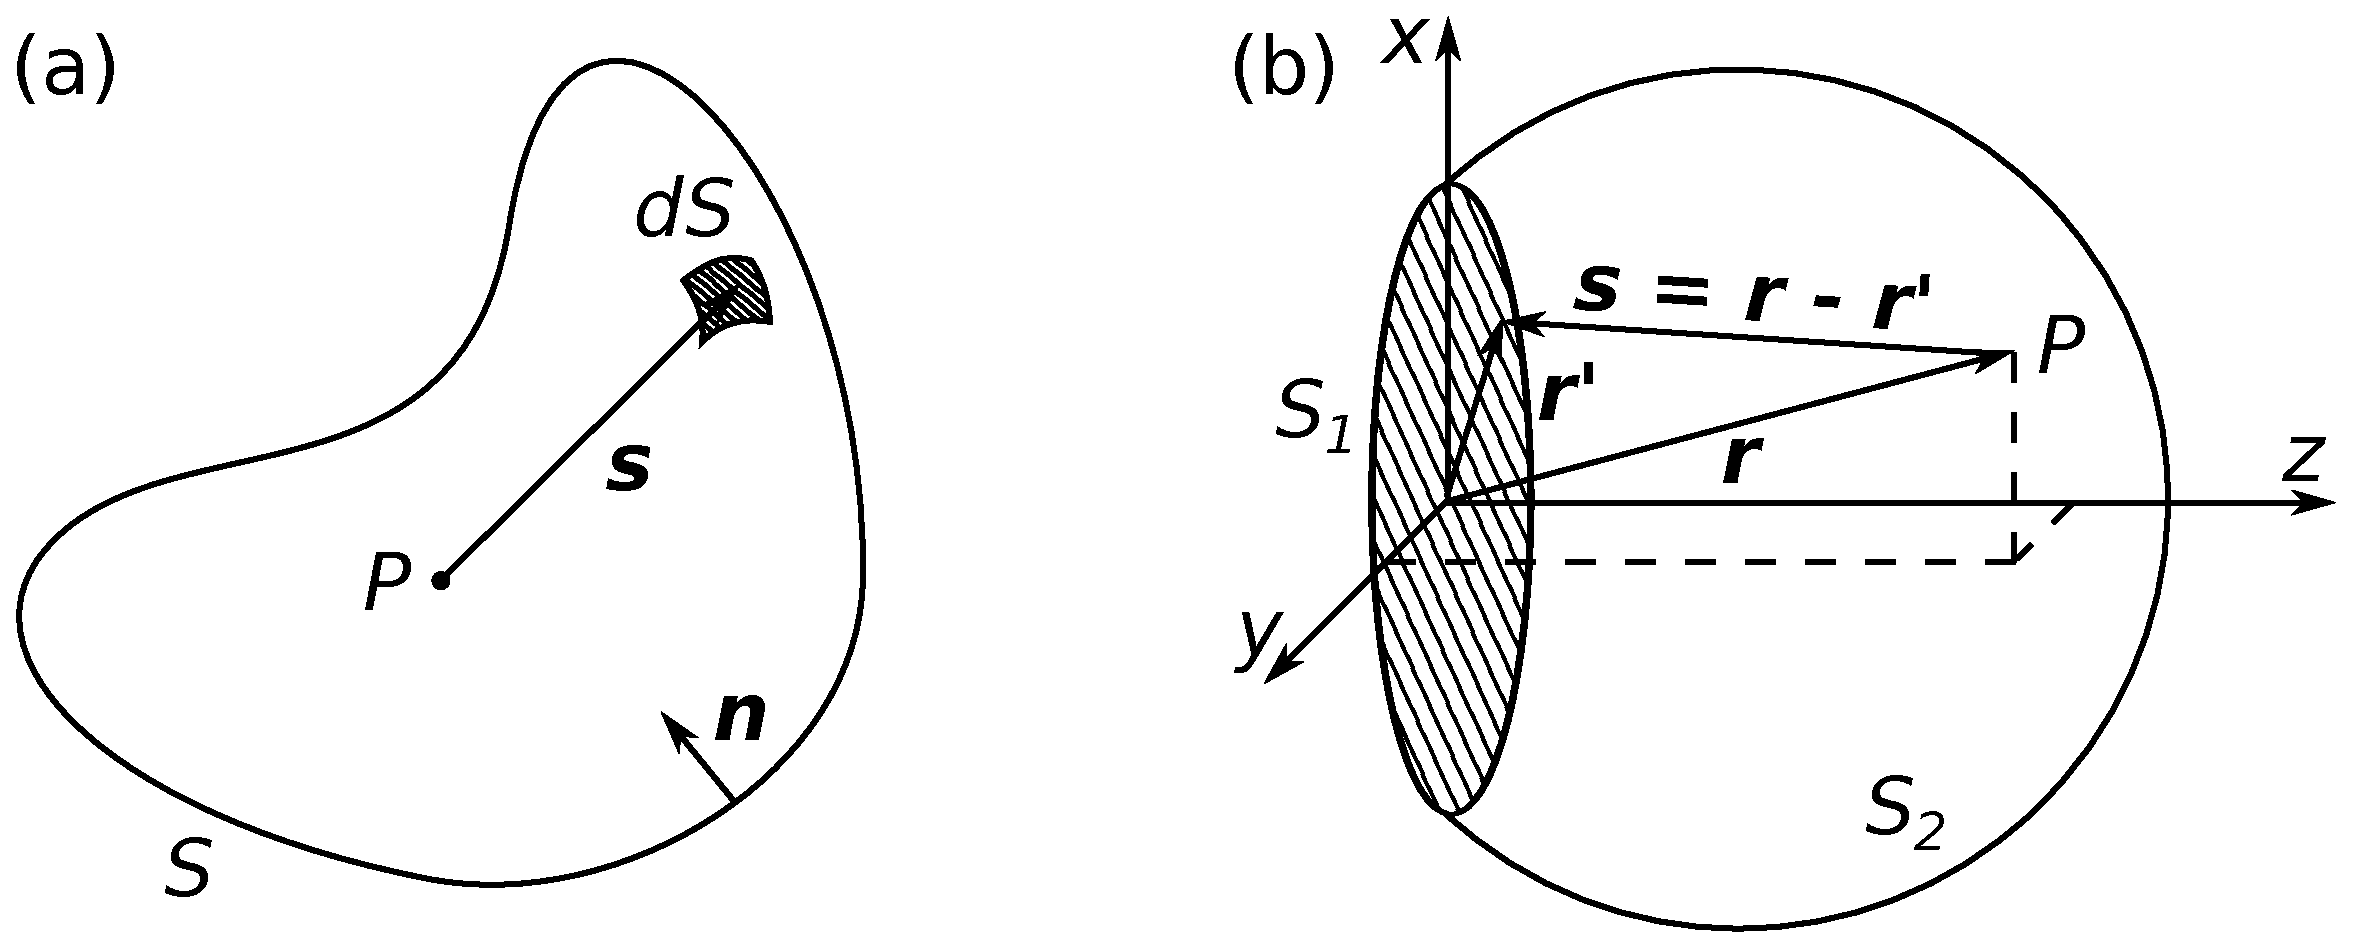
\includegraphics[width = \textwidth]{%
    Appendices/GaussianBeamDiffraction/figs/kirchhoff_geometry.eps}
  \caption[Geometries for Kirchhoff diffraction calculations]{%
    Geometries for Kirchhoff scalar-diffraction calculations.
    When $S_1$ is imaged by an optical system,
    $S_1$ is referred to as the \emph{object plane}.}
\label{fig:GaussianBeamDiffraction:Kirchhoff_geometry}
\end{figure}

To proceed with the diffraction calculation,
assume that the incident waves propagate in the $+z$-direction and
adopt the surface drawn
in Fig.~\ref{fig:GaussianBeamDiffraction:Kirchhoff_geometry}(b).
That is, $S = S_1 + S_2$,
where $S_1$ is a circle in the $(x, y)$-plane, and
$S_2$ is a spherical segment centered on the optical axis.
When $S_1$ is imaged by an optical system,
$S_1$ is referred to as the \emph{object plane}.
Now, assume that the incident waves were ``turned on''
at some finite time in the past, and
take the radius of $S_2$ to be large enough such that
none of the diffracted waves have had sufficient time to reach $S_2$,
i.e.\ $U \equiv 0$ on $S_2$.
(Of course, strictly speaking, the source's finite turn-on time
requires relaxation of the monochromatic assumption.
Finite turn-on time does not preclude a pseudo-monochromatic source, however,
and such a source is assumed hereafter).
Thus, the integral over $S_2$ vanishes, and
the diffraction calculation reduces to an integral over $S_1$.

Now, evaluation of
the Helmholtz-Kirchhoff integral
(\ref{eq:GaussianBeamDiffraction:Helmholtz_Kirchhoff_integral_theorem})
requires knowledge of $U$ on $S_1$.
For free-space propagation,
$S_1$ is an imagined (rather than a physical) surface
that does not impede the propagation of the incident wave $U^{(i)}$
(that is, $U = U^{(i)}$ and
$\partial U / \partial n = \partial U^{(i)} / \partial n$ on $S_1$).
If, however, $S_1$ contains opaque obstacles,
the free-space propagation conditions are no longer valid;
instead, the Kirchhoff boundary conditions can be adopted:
\begin{align}
  \text{surfaces of clear aperture:}&
  \quad
  U = U^{(i)},
  \quad
  \frac{\partial U}{\partial n} = \frac{\partial U^{(i)}}{\partial n},
  \notag \\
  \text{opaque surfaces:}&
  \quad \;
  U = 0,
  \qquad
  \frac{\partial U}{\partial n} = 0.
  \notag
\end{align}
While these boundary conditions are adequate for the current application,
it should be noted that they are not physical
for points that are very close to the boundaries of the opaque obstacles.


\section{Free-space diffraction of a Gaussian beam}
This section demonstrates that the Fraunhofer diffraction formalism
gives the correct form for a free-space Gaussian beam in the far-field limit,
and it also lays the groundwork for examining
the diffraction of a Gaussian beam from plasma-density fluctuations.
Note that the Gaussian-beam definition provided in
Section~\ref{sec:InterferometricMethods:Gaussian_beam_diffraction:Gaussian_beam_definition}
is used throughout the remainder of this appendix.

Assume that the incident Gaussian beam has a waist at $S_1$, and
take the radius of $S_1$ to be much larger than the beam waist $w_0$
such that the domain of integration effectively extends
over the whole $(x, y)$-plane.
For free-space propagation,
$S_1$ does not perturb the Gaussian beam; thus,
$E(\vect{r}, t) = E^{(i)}(\vect{r}, t) = E_G(\vect{r}) e^{-i \omega_0 t}$,
where $E_G(\vect{r})$ is the Gaussian beam's spatial dependence,
as defined by (\ref{eq:InterferometricMethods:Gaussian_beam}).
Now, in the far-field ($k_0 s \gg 1$) and
paraxial ($\vect{s} \approx -z \hat{\vect{z}}$) approximations
\begin{align}
  \left. \frac{e^{i k_0 s}}{s} \right|_{S_1}
  &\approx
  \frac{e^{i k_0 s}}{z},
  \notag \\
  \left. \frac{\partial}{\partial n}
  \left( \frac{e^{i k_0 s}}{s} \right) \right|_{S_1}
  &\approx
  -i k_0 \left( \frac{e^{i k_0 s}}{z} \right).
  \notag
\end{align}
The $s$-dependence in the phase arguments has been retained,
as it is the mechanism responsible for diffraction, but
the $s$-dependence in the amplitude has been dropped
as it only gives rise to negligible variations
in the amplitude of the diffracted wave.
Relative to a spherical wave,
a Gaussian beam has several additional $z$-dependencies;
however, at the beam's waist
\begin{align}
  \left. \frac{\partial w(z)}{\partial z} \right|_{\text{waist}}
  &\equiv
  0,
  \notag \\
  \left. \frac{\partial}{\partial z}
  \left[ \frac{1}{R(z)} \right] \right|_{\text{waist}}
  &=
  \frac{1}{z_R^2},
  \notag \\
  \left. \frac{\partial \psi(z)}{\partial z} \right|_{\text{waist}}
  &=
  \frac{1}{z_R}.
  \notag
\end{align}
Then, if the beam's Rayleigh range is much greater than
the probe wavelength ($k_0 z_R \gg 1$) and
the relevant transverse dimensions are much less than
the Rayleigh range ($w_0 \ll z_R$),
the Gaussian beam at $S_1$ satisfies
\begin{align}
  \left. E_G(\vect{r}') \right|_{S_1}
  &\approx
  E_0 e^{-(\rho' / w_0)^2},
  \notag \\
  \left. \frac{\partial E_G(\vect{r}')}{\partial n} \right|_{S_1}
  &\approx
  i k_0 \left[ E_0 e^{-(\rho' / w_0)^2} \right].
  \notag
\end{align}
Note that the CO$_2$ laser beams ($k_0 \approx \SI{2 \pi e5}{\per\meter}$)
that probe tokamak plasmas often have $z_R \gg \SI{10}{\meter}$
such that $k_0 z_R \gg 1$ and $w_0 \ll z_R$
(the transverse dimensions are constrained by the machine size
such that $w_0 \ll \SI{1}{\meter}$) are very well-satisfied.

Substituting the above expressions for
the incident waves and their surface-normal derivatives into
the Helmholtz-Kirchhoff integral
(\ref{eq:GaussianBeamDiffraction:Helmholtz_Kirchhoff_integral_theorem})
and simplifying yields
\begin{equation}
  E(\vect{r})
  \approx
  \frac{-i E_0}{\lambda_0 z}
  \int_{S_1}
  e^{-( \rho' / w_0 )^2}
  e^{i k_0 s}
  dS.
  \label{eq:GaussianBeamDiffraction:Kirchhoff_diffraction_integral}
\end{equation}
To proceed further, $s$ must be approximated:
\begin{align}
  s
  &=
  | \vect{\rho}' - \vect{r}|
  \notag \\
  &=
  \left[ r^2 - 2(x'x + y'y) + (x'^2 + y'^2) \right]^{1/2}
  \notag \\
  &\approx
  r - \frac{x'x + y'y}{r},
  \label{eq:GaussianBeamDiffraction:Fraunhofer_s}
\end{align}
where only terms linear in $(x' / r)$ and $(y' / r)$ have been retained.
This is known as the Fraunhofer limit, and
it is valid in the far-field $z \gg z_R$~\cite[Sec.~8.3.3]{born_and_wolf}.
Under the Fraunhofer limit
the diffraction integral
(\ref{eq:GaussianBeamDiffraction:Kirchhoff_diffraction_integral}) becomes
\begin{equation}
  E(\vect{r})
  \approx
  \frac{-i E_0}{\lambda_0 z}
  e^{i k_0 r}
  D_x D_y,
  \label{eq:GaussianBeamDiffraction:Fraunhofer_diffracted_field}
\end{equation}
where
\begin{align}
  D_x
  &=
  \int_{-\infty}^{\infty}
  e^{-( x' / w_0 )^2}
  e^{-i k_0 x' x / r}
  dx'
  \label{eq:GaussianBeamDiffraction:Fraunhofer_diffraction_integral_free_space}
  \\
  &=
  \mathcal{F} \left[%
    e^{-( x' / w_0 )^2}
  \right](k_0 x / r)
  \notag \\
  &=
  \sqrt{\pi} w_0 e^{-(k_0 w_0 x / 2 r)^2}
  \label{eq:GaussianBeamDiffraction:Fourier_transform_free_space_Gaussian}
\end{align}
gives the diffraction pattern in the $x$-direction, and
the integral has been easily evaluated by noting that
it is simply the Fourier transform of a Gaussian.
The diffraction pattern in the $y$-direction, $D_y$, is similarly determined.
Note that the $e^{-i k_0 x' x / r} = e^{-i k_0 x' \sin\theta}$ term in
(\ref{eq:GaussianBeamDiffraction:Fraunhofer_diffraction_integral_free_space})
is the typical geometric phase factor
that results from path-length differences between
points on surface $S_1$ and the field point $\vect{r}$, as shown in
Fig.~{\ref{fig:GaussianBeamDiffraction:Fraunhofer_geometric_phase_factor}}.
Substituting
(\ref{eq:GaussianBeamDiffraction:Fourier_transform_free_space_Gaussian}) into
(\ref{eq:GaussianBeamDiffraction:Fraunhofer_diffracted_field}) yields
\begin{equation}
  E(\vect{r})
  \approx
  -i E_0
  \left( \frac{z_R}{z} \right)
  e^{-(k_0 w_0 \rho / 2 r)^2}
  e^{i k_0 r}.
  \label{eq:GaussianBeamDiffraction:Fraunhofer_Gaussian_beam_diffraction}
\end{equation}
Is this consistent
with the expected far-field representation of a Gaussian beam? Yes!
To see this, note that in the far-field ($z \gg z_R$)
\begin{align}
  \frac{z_R}{z}
  &\approx
  \frac{w_0}{w(z)},
  \notag \\
  \frac{k_0 w_0 \rho}{2 r}
  &\approx
  \frac{\rho}{w(z)},
  \notag \\
  r
  &\approx
  z + \frac{\rho^2}{2 R(z)},
  \notag \\
  -i
  = e^{-i \pi / 2}
  &\approx
  e^{-i \psi(z)},
  \notag
\end{align}
such that the diffracted field in the Fraunhofer limit
(\ref{eq:GaussianBeamDiffraction:Fraunhofer_Gaussian_beam_diffraction})
can be cast in the form of a typical Gaussian beam
as expressed in
(\ref{eq:InterferometricMethods:Gaussian_beam}),
i.e.\ $E(\vect{r}) = E_G(\vect{r})$ for $z \gg z_R$.
Of course, when considering free-space propagation,
$E(\vect{r}) \equiv E_G(\vect{r})$ for $0 \leq z < \infty$, but
the above work \emph{proves} that
the Fraunhofer diffraction formalism
gives the correct results under the appropriate limits;
it also lays the groundwork for examining
the diffraction of a phase-modulated Gaussian beam.

\begin{figure}
  \centering
  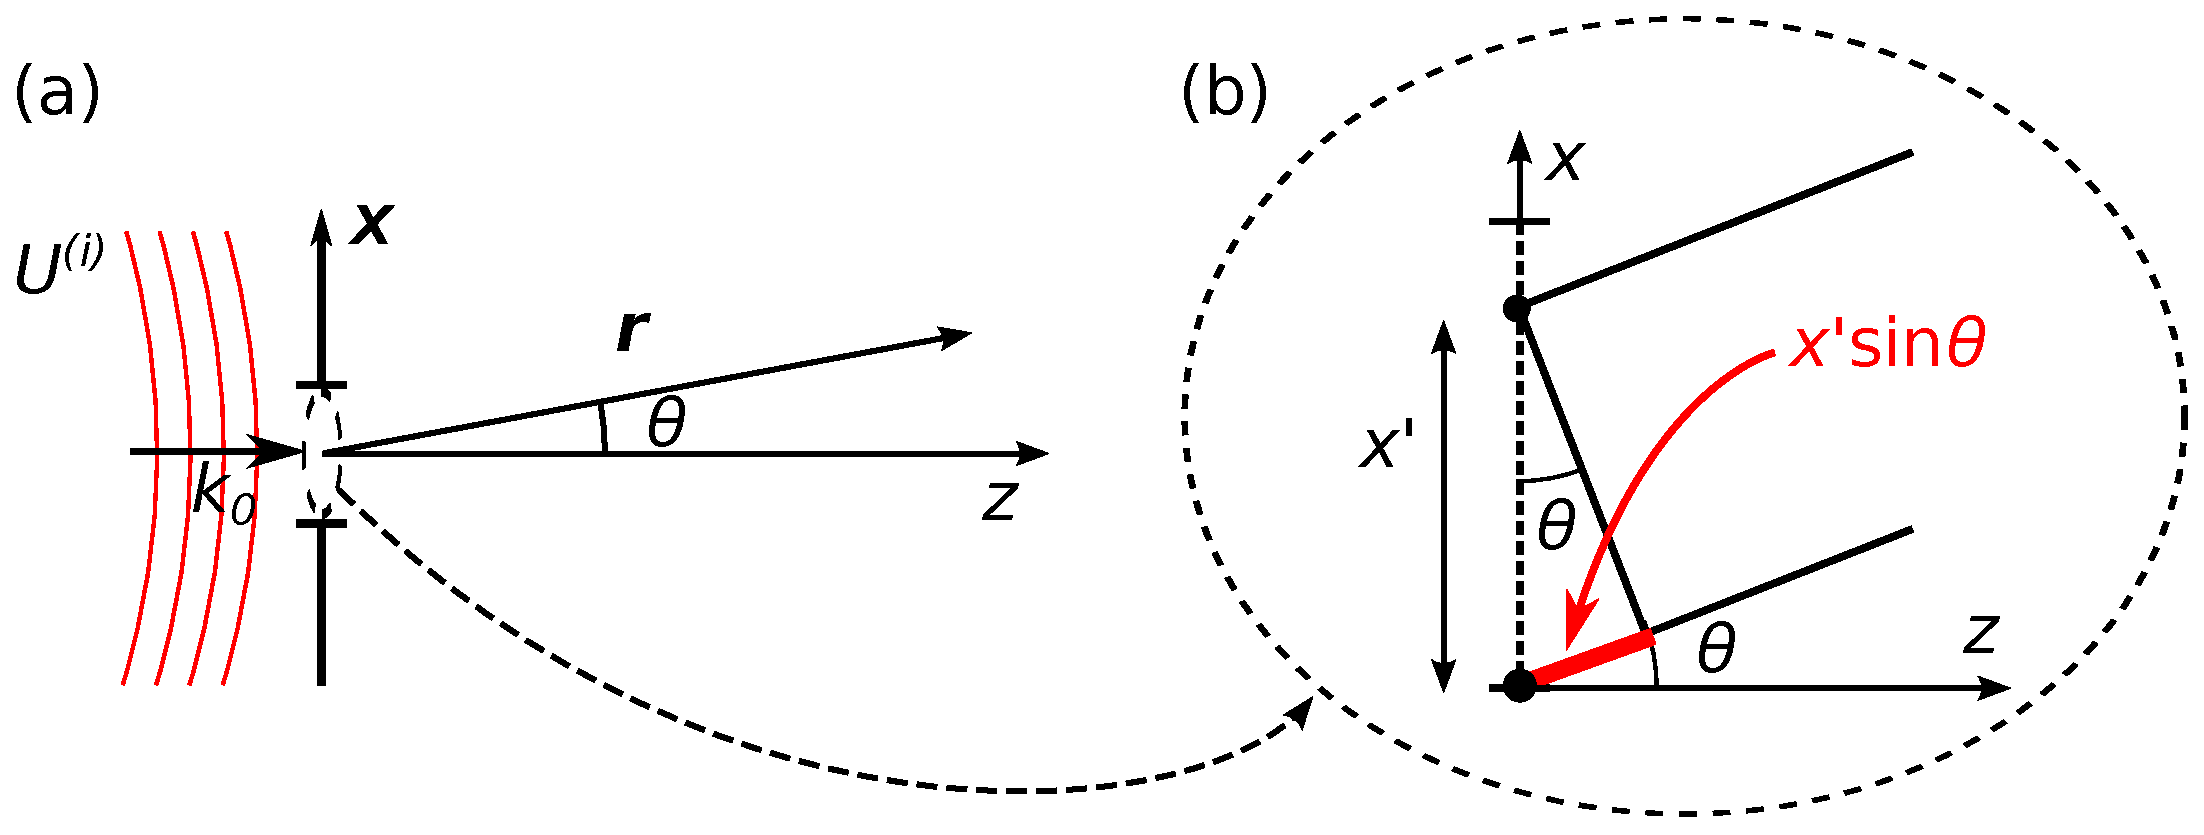
\includegraphics[width = \textwidth]{%
    Appendices/GaussianBeamDiffraction/figs/Fraunhofer_geometric_phase_factor.eps}
  \caption[Fraunhofer geometric phase factor]{%
    (a) Typical Fraunhofer diffraction geometry and
    (b) a close up that displays the path-length difference $x' \sin\theta$
    between a wave emanating from the origin and
    a wave emanating from $x'$}
\label{fig:GaussianBeamDiffraction:Fraunhofer_geometric_phase_factor}
\end{figure}


\section{Diffraction from plasma-density fluctuations}
\label{sec:GaussianBeamDiffraction:from_plasma_density_fluctuations}
Now, allow a Gaussian, CO$_2$ probe beam
to pass through a tokamak plasma.
The beam acquires the plasma-induced phase delay $\phi(\vect{\rho}', t)$
given by (\ref{eq:InterferometricMethods:phase}),
where $\vect{\rho}'$ corresponds to the beam's transverse dimensions.
Explicitly dividing $\phi$ into bulk $\bar{\phi}(t)$ and
spatially varying $\tilde{\phi}(\vect{\rho}', t)$ components,
the plasma-induced phase delay becomes
\begin{equation}
  \phi(\vect{\rho}', t) = \bar{\phi}(t) + \tilde{\phi}(\vect{\rho}', t).
\end{equation}
Typically, $\tilde{\phi}$ varies on much faster time scales than $\bar{\phi}$,
but this is not required.
The spatial variation of the plasma-induced phase delay
contributes to the diffraction of the incident Gaussian probe beam, and
the remainder of this section uses scalar-diffraction theory
to determine the diffracted field in the Fraunhofer limit;
the near-field form consistent with the computed Fraunhofer field
is then inferred.
(The object planes of the imaging systems relevant to this work
sit in the near field, so computation of the imaged field requires
knowledge of the near-field diffraction pattern).

The response functions of the diagnostics investigated in
Sections~\ref{sec:InterferometricMethods:interferometry} and
\ref{sec:InterferometricMethods:pci} are shown
to be linear in their regimes of relevance, so
it is sufficient to examine phase fluctuations $\tilde{\phi}$
consisting of a single Fourier mode
\begin{equation}
  \tilde{\phi}(\vect{\rho}', t) = \tilde{\phi}_0 \cos(k x' - \omega t).
  \label{eq:GaussianBeamDiffraction:cosine_phase_fluctuation}
\end{equation}
As a CO$_2$ beam's optical cycles
($\omega_0 = 2 \pi \cdot \SI{28.3}{\tera\hertz}$)
occur much more rapidly than the temporal evolution of the plasma
($\omega \lesssim 2 \pi \cdot \SI{1}{\giga\hertz}$),
the problem can be treated adiabatically
by solving for the beam propagation
at each instant in time during the relatively slow evolution of $\phi$.
Then, following the formalism pioneered by Raman and Nath
\cite{raman_nath_diffraction_partI,raman_nath_diffraction_partIII},
this plasma-induced phase delay makes an additional phase contribution
to the diffraction integral
(\ref{eq:GaussianBeamDiffraction:Fraunhofer_diffraction_integral_free_space})
such that the diffraction pattern in the $x$-direction is given as
\begin{align}
  D_x
  &=
  \int_{-\infty}^{\infty}
  e^{-( x' / w_0 )^2}
  e^{-i k_0 x x' / r}
  e^{i \phi(x', t)}
  dx'
  \notag \\
  &=
  e^{i \bar{\phi}}
  \int_{-\infty}^{\infty}
  e^{-( x' / w_0 )^2}
  e^{-i k_0 x x' / r}
  e^{i \tilde{\phi}_0 \cos(k x' - \omega t)}
  dx'
  \notag \\
  &\begin{aligned}
    =
    e^{i \bar{\phi}}
    &\int_{-\infty}^{\infty}
    e^{-( x' / w_0 )^2}
    e^{-i k_0 x x' / r}
    \\
    &\times
    \left\{%
      \sum_{m = -\infty}^{\infty}
      i^m \left[ J_m(\tilde{\phi}_0) \right]
      e^{i m (k x' - \omega t)}
    \right\}
    dx'
  \end{aligned}
  \notag \\
  &\begin{aligned}
    =
    e^{i \bar{\phi}}
    &\sum_{m = -\infty}^{\infty}
    i^m \left[ J_m(\tilde{\phi}_0) \right]
    e^{-i m \omega t}
    \\
    &\times
    \int_{-\infty}^{\infty}
    e^{-( x' / w_0 )^2}
    e^{-i \left( \frac{k_0 x}{r} - m k \right) x'}
    dx'
  \end{aligned}
  \notag \\
  &\begin{aligned}
    =
    \sqrt{\pi} w_0
    e^{i \bar{\phi}}
    \sum_{m = -\infty}^{\infty}
    \biggl\{
      &i^m \left[ J_m(\tilde{\phi}_0) \right]
      e^{-i m \omega t}
      \\
      &\qquad \times
      e^{-\left[ \frac{w_0}{2} \left( \frac{k_0 x}{r} - m k \right) \right]^2}
    \biggr\},
  \end{aligned}
  \label{eq:GaussianBeamDiffraction:Fraunhofer_diffraction_integral_phase_modulated}
\end{align}
where the bracketed expression in the third equality follows from
application of the well-known Jacobi-Anger expansion and
$J_m$ is the $m$\ts{th} Bessel function of the first kind.
Noting that $E(\vect{r}, t) = E(\vect{r}) e^{-i \omega_0 t}$,
substitution of
(\ref{eq:GaussianBeamDiffraction:Fraunhofer_diffraction_integral_phase_modulated})
into (\ref{eq:GaussianBeamDiffraction:Fraunhofer_diffracted_field}) yields
\begin{align}
  \begin{aligned}
    E(\vect{r}, t)
    \approx
    &\sum_{m = -1}^{1}
    i^m \left[ J_m(\tilde{\phi}_0) \right]
    e^{-i m \omega t}
    e^{-\left[ \frac{w_0}{2} \left( \frac{k_0 x}{r} - m k \right) \right]^2}
    \\
    &\times
    e^{i \bar{\phi}}
    \left[
      -i E_0
      \left( \frac{z_R}{z} \right)
      e^{-(k_0 w_0 y / 2 r)^2}
      e^{i (k_0 r - \omega_0 t)}
    \right].
  \label{eq:GaussianBeamDiffraction:Fraunhofer_phase_modulated_Gaussian_beam_diffraction}
  \end{aligned}
\end{align}
Here, only the $|m| \leq 1$ terms have been retained because
$|J_m(\tilde{\phi}_0)| \sim \tilde{\phi}_0^{|m|}$
for experimentally relevant values of $\tilde{\phi}_0 \ll 1$.
(The complete small-argument, asymptotic form for $J_m$ is discussed in
Section~\ref{sec:InterferometricMethods:imaging:weak_coupling_limit}).
The effect of higher order terms can be easily investigated
by e.g.\ including the $m = \pm 2$ terms etc.

\begin{figure}
  \centering
  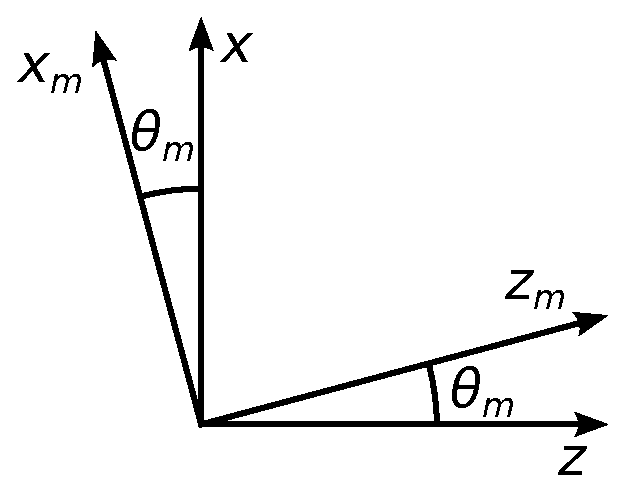
\includegraphics[width = 0.4 \textwidth]{%
    Appendices/GaussianBeamDiffraction/figs/coordinate_rotation.eps}
  \caption{Coordinate transformation for interpretation of
    the diffraction pattern of a phase-modulated Gaussian beam}
\label{fig:GaussianBeamDiffraction:coordinate_rotation}
\end{figure}

To put
(\ref{eq:GaussianBeamDiffraction:Fraunhofer_phase_modulated_Gaussian_beam_diffraction})
in a more familiar form,
consider the coordinate transformation
from the lab-frame coordinate system $\vect{r}$
to the coordinate system of the $m$\ts{th} scattered beam $\vect{r}_m$,
as depicted graphically
in Fig.~\ref{fig:GaussianBeamDiffraction:coordinate_rotation}.
As the transformation is simply
a rotation about the $y$-axis by angle $\theta_m$,
the coordinate systems are related via
\begin{equation}
  \begin{pmatrix}
    x_m
    \\
    y_m
    \\
    z_m
  \end{pmatrix}
  =
  \begin{pmatrix}
    \cos\theta_m & 0 & -\sin\theta_m
    \\
    0            & 1 & 0
    \\
    \sin\theta_m & 0 & \cos\theta_m
  \end{pmatrix}
  \begin{pmatrix}
    x
    \\
    y
    \\
    z
  \end{pmatrix},
  \label{eq:GaussianBeamDiffraction:object_plane_coordinate_transformation_explicit}
\end{equation}
where
\begin{equation}
  \sin \theta_m
  \equiv
  \frac{m k}{k_0}.
  \label{eq:GaussianBeamDiffraction:scattering_angles}
\end{equation}
Typically, $m k / k_0 \ll 1$ such that
\begin{equation}
  \cos \theta_m
  \approx
  1 - \frac{1}{2} \left( \frac{m k}{k_0} \right)^2
\end{equation}
is a very good approximation.
The above coordinate transformation can be written more compactly as
\begin{equation}
  \vect{r}_m
  =
  [ \vect{R}(\theta_m) ] \vect{r},
  \label{eq:GaussianBeamDiffraction:object_plane_coordinate_transformation_compact}
\end{equation}
where
\begin{equation}
  \vect{R}(\theta)
  =
  \begin{pmatrix}
    \cos\theta & 0 & -\sin\theta
    \\
    0          & 1 & 0
    \\
    \sin\theta & 0 & \cos\theta
  \end{pmatrix}
  \label{eq:GaussianBeamDiffraction:rotation_matrix}
\end{equation}
is the rotation matrix
that rotates the $(x, z)$-plane about the $y$-axis by angle $\theta$.
Rotation matrices are \emph{orthogonal},
which endows $\vect{R}(\theta_m)$ with some useful properties
\cite[Ch.~6]{FB_linear_algebra};
namely, its inverse is equal to its transpose $[\vect{R}(\theta_m)]^T$
\begin{equation}
  [\vect{R}(\theta_m)]^T
  =
  [\vect{R}(\theta_m)]^{-1}
  =
  \vect{R}(-\theta_m),
  \label{eq:GaussianBeamDiffraction:rotation_matrix_inverse_relationships}
\end{equation}
and its determinant is unity
\begin{equation}
  \text{det}[\vect{R}(\theta_m)] = |\vect{R}(\theta_m)| = 1
  \label{eq:GaussianBeamDiffraction:rotation_matrix_determinant}
\end{equation}
such that the rotation preserves lengths, i.e.\ $r_m = r$.
It is sufficient to retain terms only to first order in
$k / k_0$ (small scattering angle) and $x / z$ (paraxial limit)
for the \emph{amplitude} dependencies of the diffracted field
(this is \emph{not}, in general, true for the phase dependencies).
Thus, $1 / z \approx 1 / z_m$ and $x \approx x_m + (m k / k_0) z$
such that the Fraunhofer diffracted field
(\ref{eq:GaussianBeamDiffraction:Fraunhofer_phase_modulated_Gaussian_beam_diffraction})
can be rewritten as
\begin{equation}
  \begin{aligned}
    E(\vect{r}, t)
    \approx
    e^{i \bar{\phi}}
    &\sum_{m = -1}^{1}
    i^m \left[ J_m(\tilde{\phi}_0) \right]
    e^{-i (\omega_0 + m \omega) t}
    \\
    &\times
    \left[
      -i E_0
      \left( \frac{z_R}{z_m} \right)
      e^{-(k_0 w_0 \rho_m / 2 r)^2}
      e^{i k_0 r}
    \right],
  \end{aligned}
\end{equation}
where $\rho_m = (x_m^2 + y_m^2)^{1/2}$.
Now, the bracketed expression has the form of
(\ref{eq:GaussianBeamDiffraction:Fraunhofer_Gaussian_beam_diffraction})
for a far-field Gaussian beam; thus,
the diffracted electric field can be more compactly and generally written as
\begin{equation}
  E(\vect{r}, t)
  \approx
  e^{i \bar{\phi}}
  \sum_{m = -1}^{1}
  i^m \left[ J_m(\tilde{\phi}_0) \right]
  E_G(\vect{r}_m)
  e^{-i (\omega_0 + m \omega) t}.
  \label{eq:GaussianBeamDiffraction:phase_modulated_Gaussian_beam_diffraction}
\end{equation}
Note that
(\ref{eq:GaussianBeamDiffraction:phase_modulated_Gaussian_beam_diffraction})
is valid for $0 \leq z < \infty$ rather than only for $z \gg z_R$;
that is, computing the far-field diffraction pattern
has additionally allowed \emph{inferring} the corresponding near field.

Thus, a sinusoidal phase modulation diffracts an incident Gaussian beam
predominantly into downscattered ($m = -1$), unscattered ($m = 0$), and
upscattered ($m = 1$) Gaussian beams.
The incident beam is coupled into the $m$\ts{th} scattered beam
with strength $J_m(\tilde{\phi}_0)$.
The $m$\ts{th} scattered beam is Doppler shifted
relative to the incident beam by $m \omega$ and
propagates at an angle $\theta_m \approx m k / k_0$
relative to the lab-frame optical axis.
The adiabatic assumption ($\omega / \omega_0 \ll 1$)
is very well-satisfied for a CO$_2$ probe beam
in a typical tokamak plasma
(i.e.\
$\omega / \omega_0
\lesssim
\SI{1}{\giga\hertz} / \SI{28.3}{\tera\hertz}
\sim 10^{-5}$).
Thus, the scattering is very nearly elastic, and
$|\vect{k}_{0,m}| = k_0$ is a very good approximation.
This constraint of elasticity
coupled with knowledge of the scattering angle $\theta_m$
allows determination of the scattered wavevector
\begin{equation}
  \vect{k}_{0,m}
  =
  (m k) \hat{\vect{x}}
  +
  k_0 \left[ 1 - \left(\frac{m k}{k_0}\right)^2 \right]^{1/2} \hat{\vect{z}}.
  %k_0 \sqrt{1 - \left(\frac{m k}{k_0}\right)^2} \hat{\vect{z}}
  \label{eq:GaussianBeamDiffraction:scattered_beam_wavevector}
\end{equation}
Finally, note that the simultaneous presence
of both the upscattered and downscattered beams
under typical experimental conditions
has been demonstrated empirically
\cite[Sec.~2.1]{dorris_phd}.
In the above formalism, the simultaneous upscattering and downscattering
of the incident probe beam results from
the assumption of a sinusoidal phase fluctuation in
(\ref{eq:GaussianBeamDiffraction:cosine_phase_fluctuation});
if a complex exponential were assumed instead,
one would erroneously deduce that
only one such scattering process (either up or down) occurs.


\section{Validity of the Raman-Nath formalism}
The Raman-Nath formalism employed in
Section~\ref{sec:GaussianBeamDiffraction:from_plasma_density_fluctuations}
is valid as long as the fluctuation wavenumber $k$ is not ``too large''.
This constraint has been rigorously quantified by Bhatia and Noble
\cite{bhatia_53_general_theory,bhatia_53_approximate_expressions_for_intensities} and
is also discussed by Born and Wolf
\cite[Ch.~12]{born_and_wolf}.
Specifically, beam diffraction will be in the Raman-Nath regime when
\begin{equation}
  \delta = \frac{\tilde{n}_e}{\bar{n}_e} \left( \frac{k_0}{k} \right)^2 \gg 1,
  \label{eq:GaussianBeamDiffraction:raman_nath_validity_criterion}
\end{equation}
where
$\bar{n}_e$ is the bulk plasma density,
$\tilde{n}_e$ is the amplitude of the plasma-density fluctuation,
$k_0$ is the vacuum wavenumber of the probe beam, and
$k$ is the wavenumber of the plasma-density fluctuation.
Note that the above $\delta$ is equivalent
to that used by Bhatia and Noble,
after having made the appropriate substitutions
for a CO$_2$ probe beam in a tokamak plasma.
Assuming typical tokamak values
\begin{align}
  &\frac{\tilde{n}_e}{\bar{n}_e}
  \sim
  10^{-3},
  \notag \\
  &k
  \lesssim
  \SI{30}{\per\centi\meter}
  \notag
\end{align}
yields $\delta \gtrsim 40$
for a CO$_2$ probe beam ($k_0 \approx 2 \pi \cdot \SI{e5}{\per\meter}$)
such that beam's diffraction is well within the Raman-Nath regime.
In the opposite regime ($\delta \ll 1$)
the beam can \emph{Bragg scatter} from the phase fluctuation,
producing a single, strongly-scattered beam
\cite{bhatia_53_approximate_expressions_for_intensities}
\cite[Ch.~12]{born_and_wolf};
such Bragg scattering is the foundation of acousto-optics.


\section{Wavenumber filtering of the diffracted field}
Examine again the diffracted field
(\ref{eq:GaussianBeamDiffraction:phase_modulated_Gaussian_beam_diffraction}).
The spatial dependence of each term in the summation
is wholly governed by the factor $E_G(\vect{r}_m)$,
which corresponds to a Gaussian beam
that emanates from the beam waist
at an angle $\theta_m$ relative to the lab-frame $z$-axis.
The coordinate system $\vect{r}_m$ is defined such that
the $m$\ts{th} Gaussian beam propagates along the $z_m$-axis, and
it is related to the lab-frame coordinate system $\vect{r}$ via
(\ref{eq:GaussianBeamDiffraction:object_plane_coordinate_transformation_compact}).
The wavenumber basis $\vect{k}_m$ that is dual to $\vect{r}_m$
is similarly related to the lab-frame wavenumber basis $\vect{k}$ via
\begin{equation}
  \vect{k}_m
  =
  [ \vect{R}(\theta_m) ] \vect{k},
  \label{eq:GaussianBeamDiffraction:object_plane_coordinate_transformation_wavenumber_dual}
\end{equation}
which naturally results from the geometric constraint that
$\vect{k} \cdot \vect{r} = \vect{k}_m \cdot \vect{r}_m$.

Imagine now that each of the above Gaussian beams
is somehow manipulated based upon its Fourier wavenumber content.
Assume this manipulation can be described
in terms of a transfer function $T(\vect{k})$,
where $\vect{k}$ is the lab-frame wavenumber basis.
A transfer function of this form is appropriate for investigating e.g.\
diffraction from an aperture or the action of a phase plate.
Using the wavenumber basis transformation
(\ref{eq:GaussianBeamDiffraction:object_plane_coordinate_transformation_wavenumber_dual}),
this transfer function can be written
in terms of the $\vect{k}_m$ wavenumber basis as
\begin{equation}
  T(\vect{k}) = T(\vect{R}_{-m} \vect{k}_m),
\end{equation}
where the abbreviation $\vect{R}_m = \vect{R}(\theta_m)$ has been adopted.
The transformed field $E_T$ then has the Fourier representation
in the $\vect{k}_m$ wavenumber basis
\begin{equation}
  E_T(\vect{k}_m) = T(\vect{R}_{-m} \vect{k}_m) \cdot E_G(\vect{k}_m).
\end{equation}
Inverse Fourier transforming $E_T(\vect{k}_m)$ yields
\begin{equation}
  E_T(\vect{r}_m)
  =
  \frac{1}{(2 \pi)^3}
  \int d\vect{k}_m \,
  \left[%
    T(\vect{R}_{-m} \vect{k}_m)
    e^{i \vect{k}_m \cdot \vect{r}_m}
  \right]
  E_G(\vect{k}_m).
\end{equation}
Note that each spectral component $E_G(\vect{k}_m)$
individually satisfies the wave equation.
Thus, the above construction of the transformed field $E_T(\vect{r}_m)$,
which consists of a linear combination of the spectral components
with arbitrary amplitudes and phases,
\emph{also} satisfies the wave equation.
Now, explicitly writing $E_G(\vect{k}_m)$ as the Fourier transform
of $E_G$ over a dummy spatial coordinate $\vect{r}'$, and
exchanging the order of integration yields
\begin{equation}
  E_T(\vect{r}_m)
  =
  \frac{1}{(2 \pi)^3}
  \int d\vect{r}' \,
  E_G(\vect{r}')
  \int d\vect{k}_m \,
  T(\vect{R}_{-m} \vect{k}_m)
  e^{i \vect{k}_m \cdot (\vect{r}_m - \vect{r}')}.
\end{equation}
Further, for the applications considered here,
it is advantageous to change the variables of integration
from the $\vect{k}_m$ wavenumber basis
to the lab-frame wavenumber basis $\vect{k}$.
Note that
\begin{equation}
  d\vect{k}_m
  =
  \left| \frac{\partial \vect{k}_m}{\partial \vect{k}} \right|
  d\vect{k}
  =
  |\vect{R}_m|
  d\vect{k}
  =
  d\vect{k}
\end{equation}
and that
\begin{align}
  \vect{k}_m \cdot (\vect{r}_m - \vect{r}')
  &=
  (\vect{R}_m \vect{k}) \cdot (\vect{r}_m - \vect{r}')
  \notag \\
  &=
  (\vect{R}_m \vect{k})^T (\vect{r}_m - \vect{r}')
  \notag \\
  &=
  \vect{k}^T \vect{R}_m^T (\vect{r}_m - \vect{r}')
  \notag \\
  &=
  \vect{k} \cdot [\vect{R}_{-m} (\vect{r}_m - \vect{r}')]
\end{align}
such that the transformed field $E_T(\vect{r}_m)$ becomes
\begin{equation}
  E_T(\vect{r}_m)
  =
  \frac{1}{(2 \pi)^3}
  \int d\vect{r}' \,
  E_G(\vect{r}')
  \int d\vect{k} \,
  T(\vect{k})
  e^{i \vect{k} \cdot \left[ \vect{R}_{-m} (\vect{r}_m - \vect{r}') \right]},
  \label{eq:GaussianBeamDiffraction:mth_diffracted_beam_Fourier_filtered}
\end{equation}
where, again, the abbreviation $\vect{R}_{-m} = \vect{R}(-\theta_m)$
has been adopted and $\vect{R}(\theta)$ is the rotation matrix given by
(\ref{eq:GaussianBeamDiffraction:rotation_matrix}).

To make further progress,
a particular form of $T(\vect{k})$ is needed.
Assume that wavenumbers are filtered
only in the direction of beam scattering
i.e.\ $T(\vect{k}) = T(k_x)$.
(For example, the groove of a phase plate would be aligned
with the lab-frame $y$-axis to effect such filtering).
Then
\begin{equation}
  \vect{R}_{-m} (\vect{r}_m - \vect{r}')
  =
  \begin{pmatrix}
    (x_m - x') \cos\theta_m + (z_m - z') \sin\theta_m
    \\
    y_m - y'
    \\
    (z_m - z') \cos\theta_m - (x_m - x') \sin\theta_m
  \end{pmatrix}
\end{equation}
such that
(\ref{eq:GaussianBeamDiffraction:mth_diffracted_beam_Fourier_filtered})
becomes
\begin{align}
  E_T(\vect{r}_m)
  &=
  \frac{1}{(2 \pi)^3}
  \int d\vect{r}' \,
  E_G(\vect{r}')
  \int dk_y \,
  e^{i k_y (y_m - y')}
  \notag \\
  &\qquad\quad \times
  \int dk_z \,
  e^{i k_z [(z_m - z') \cos\theta_m - (x_m - x') \sin\theta_m]}
  \notag \\
  &\qquad\quad \times
  \int dk_x \,
  T(k_x)
  e^{i k_x \left[ (x_m - x') \cos\theta_m + (z_m - z') \sin\theta_m \right]}
  \notag \\
  &=
  \frac{1}{2 \pi}
  \int d\vect{r}' \,
  E_G(\vect{r}')
  \delta(y_m - y')
  \notag \\
  &\qquad\quad \times
  \delta\bigl( (z_m - z') \cos\theta_m - (x_m - x') \sin\theta_m \bigr)
  \notag \\
  &\qquad\quad \times
  \int dk_x \,
  T(k_x)
  e^{i k_x \left[ (x_m - x') \cos\theta_m + (z_m - z') \sin\theta_m \right]}
  \notag \\
  &\begin{aligned}
    &=
    \frac{1}{2 \pi}
    \int dx' \,
    E_G\bigl( x',\, y_m,\, z_m - (x_m - x')\tan \theta_m \bigr)
    \\
    &\qquad\quad \times
    \int dk_x \,
    T(k_x)
    e^{i k_x (x_m - x') \sec\theta_m}
  \end{aligned}
  \label{eq:GaussianBeamDiffraction:mth_diffracted_beam_kx_filtered_v1}
\end{align}
Contributions to the integral from regions outside of $|x'| \lesssim w(z_m)$
are suppressed by the Gaussian envelope such that
\begin{align}
  w\bigl( z_m - (x_m - x')\tan \theta_m \bigr)
  &\approx
  w(z_m),
  \notag \\
  R\bigl( z_m - (x_m - x')\tan \theta_m \bigr)
  &\approx
  R(z_m),
  \notag \\
  \psi\bigl( z_m - (x_m - x')\tan \theta_m \bigr)
  &\approx
  \psi(z_m)
  \notag
\end{align}
are very good approximations.
Note that the phase of the Gaussian beam
\emph{cannot} be approximated in such a manner;
instead, terms up to first order in $\theta_m$
must be retained in the phase.
After making these approximations,
(\ref{eq:GaussianBeamDiffraction:mth_diffracted_beam_kx_filtered_v1})
reduces to
\begin{equation}
  E_T(\vect{r}_m)
  \approx
  E_G(0, y_m, z_m)
  \cdot
  \mathcal{E}(\vect{r}_m, k),
  \label{eq:GaussianBeamDiffraction:mth_diffracted_beam_kx_filtered_compact}
\end{equation}
where
\begin{equation}
  \begin{aligned}
    \mathcal{E}(\vect{r}_m, k)
    &=
    \frac{e^{-i m k x_m}}{2 \pi}
    \\
    &\quad \times
    \int dx' \,
    \exp\left[ \frac{-x'^2}{w(z_m)^2} \right]
    \exp\left\{%
      i \left[%
        m k x'
        +
        \frac{k_0 x'^2}{2 R(z_m)}
      \right]
    \right\}
    \\
    &\quad \times
    \int dk_x \,
    T(k_x)
    e^{i k_x (x_m - x')}
  \end{aligned}
  \label{eq:GaussianBeamDiffraction:mth_diffracted_beam_kx_filtered_transformation}
\end{equation}
is a complex-valued function
that describes the amplitude and phase transformations
that result from filtering the scattered radiation by $T(k_x)$.
(Note that
(\ref{eq:GaussianBeamDiffraction:mth_diffracted_beam_kx_filtered_compact})
readily reduces to $E_T(\vect{r}_m) = E_G(\vect{r}_m)$ when $T(k_x) = 1$,
in agreement with expectations).
Generalizing
(\ref{eq:GaussianBeamDiffraction:phase_modulated_Gaussian_beam_diffraction})
to allow for such wavenumber-dependent manipulation
yields a total diffracted electric field
\begin{equation}
  E(\vect{r}, t)
  \approx
  e^{i \bar{\phi}}
  \sum_{m = -1}^{1}
  i^m \left[ J_m(\tilde{\phi}_0) \right]
  E_T(\vect{r}_m)
  e^{-i (\omega_0 + m \omega) t}.
  \label{eq:GaussianBeamDiffraction:phase_modulated_Gaussian_beam_diffraction_Fourier_filtered}
\end{equation}
Manipulating the total diffracted electric field in such a manner
forms the foundation of phase contrast imaging (PCI),
as is discussed in Section~\ref{sec:InterferometricMethods:pci}.


\bibliographystyle{plainurl}
\bibliography{references}
%
\chapter{Imaging systems}
\label{app:ImagingSystems}


\section{Geometric optics of imaging systems}
Let the optical axis of an arbitrary optical system lie along the $z$-axis,
and let all optical rays lie in a plane with the optical axis.
At a given position $z_j$, an optical ray is fully described by
its transverse distance $\rho$ to the optical axis and
its slope $d\rho / dz$.
In the paraxial limit $d\rho / dz \approx \theta$,
where $\theta$ is the angle between the ray and the optical axis.
Ray propagation through homogeneous media and refractive interfaces
is well-governed by the so-called $ABCD$ ray-matrix formalism
\cite[Ch.~15]{siegman_lasers};
that is, a ray propagating from point $j$ to point $j + 1$ evolves as
\begin{equation}
  \begin{pmatrix}
    \rho_{j + 1}
    \\
    \theta_{j + 1}
  \end{pmatrix}
  =
  \begin{pmatrix}
    A & B
    \\
    C & D
  \end{pmatrix}
  \begin{pmatrix}
    \rho_j
    \\
    \theta_j
  \end{pmatrix},
  \label{eq:ImagingSystems:ABCD_ray_tracing_general}
\end{equation}
where the $ABCD$ matrix elements are determined
by the optical properties of the media between points $j$ and $j + 1$.
Some rudimentary $ABCD$ matrices are given in
Table~\ref{table:ImagingSystems:ABCD_matrices}, while
more exhaustive lists can be readily found elsewhere
\cite[Ch.~15]{siegman_lasers}~\cite{tovar_generalized_beam_matrices_IV}.

\begin{table}
  \centering
  \renewcommand{\arraystretch}{1.5}% Spread rows out...
  \begin{tabular}{%
    >{\centering}m{6cm} >{\centering}m{4.5cm}
  }
    \toprule%
    \textbf{optical element} & $\mathbf{ABCD}$~\textbf{matrix}
    \tabularnewline%
    \midrule
    \textbf{propagation} by distance $d$ \\
    through medium of constant \\
    index of refraction, $N$
    &
    $\begin{pmatrix}
      1 & d
      \\
      \phantom{-} 0 \phantom{f} & 1  % phantoms to match thin lens format
    \end{pmatrix}$
    \tabularnewline%
    \textbf{thin lens} with \\
    focal length $f$
    &
    $\begin{pmatrix}
      1 & 0
      \\
      -1/f & 1
    \end{pmatrix}$
    \tabularnewline%
    \toprule%
  \end{tabular}
  \caption[Some $ABCD$ ray matrices]{Some useful $ABCD$ ray matrices.}
\label{table:ImagingSystems:ABCD_matrices}
\end{table}

An imaging system $\image$, by definition,
redirects all rays emanating from transverse position $\rho_{\object}$
in the object plane $S_{\object}$
to intersect at transverse position
\begin{equation}
  \rho_{\image} = M \rho_{\object}
  \label{eq:ImagingSystems:image_plane_transverse_coordinates}
\end{equation}
in the image plane $S_{\image}$.
Here, $M$ is the \emph{magnification} of the imaging system, and
$M < 0$ implies that the image is inverted relative to the object.
The imaging system's $A$, $B$, and $D$ matrix elements
are easily determined by inspection.
Recalling the ray-matrix definitions in
(\ref{eq:ImagingSystems:ABCD_ray_tracing_general}),
note that
$\rho_{\image} = M \rho_{\object} = A \rho_{\object} + B \theta_{\object}$
such that $A = M$ and $B = 0$.
Further, assuming the image plane and object plane refractive indices
are identical, as is often the case,
the determinant of the ray matrix is unity
(i.e.\ $AD - BC = 1$)~\cite{halbach_63}
such that $D = 1 / M$.
The final matrix element $C$ is determined by the particulars
of the imaging system;
for propagation through ``simple'' optical components,
such as lenses and homogeneous media, $C$ is constrained to be real.
Thus, an imaging system of magnification $M$ is characterized
by an $ABCD$ ray matrix of the form
\begin{equation}
  \mathcal{I}
  =
  \begin{pmatrix}
    M & 0
    \\
    C & 1 / M
  \end{pmatrix}.
  \label{eq:ImagingSystems:ABCD_imaging}
\end{equation}

The symmetry axis of a Gaussian beam
behaves as a ray in the geometric-optics sense
\cite{tovar_generalized_beam_matrices_IV}.
Application of the imaging $ABCD$ ray matrix
(\ref{eq:ImagingSystems:ABCD_imaging})
to a beam scattered by $\theta_m$ in the object plane
(i.e.\ see (\ref{eq:InterferometricMethods:scattered_beam_wavevector}))
indicates that this beam will be rotated by angle $\theta_m / M$
relative to the unscattered beam in the image plane,
as shown in Fig.~\ref{fig:ImagingSystems:imaging_geometry}.
Further, the imaging optics do \emph{not} alter
the magnitude of the beam's wavevector, i.e.\ $|\image(\vect{k}_m)| = k_0$
(this readily follows from the fact that the imaging optics
do not alter the energy of the beam's constituent photons).
Knowledge of the wavevector's image-plane magnitude and orientation
allows determination of the image-plane wavevector as
\begin{align}
  \image(\vect{k}_{0,m})
  =
  \vect{k}_{0,m,\image}
  =
  \left( m k_{\image} \right) \hat{\vect{x}}
  +
  k_0 \left[ 1 - \left(\frac{m k_{\image}}{k_0}\right)^2 \right]^{1/2}
  \hat{\vect{z}},
  \label{eq:ImagingSystems:scattered_beam_wavevector_image_plane}
\end{align}
where
\begin{equation}
  k_{\image} \equiv \frac{k}{M}
  \label{eq:ImagingSystems:image_plane_fluctuation_wavenumber}
\end{equation}
is the \emph{imaged} wavenumber
of the corresponding object-plane phase fluctuation
(\ref{eq:InterferometricMethods:cosine_phase_fluctuation}).

\begin{figure}
  \centering
  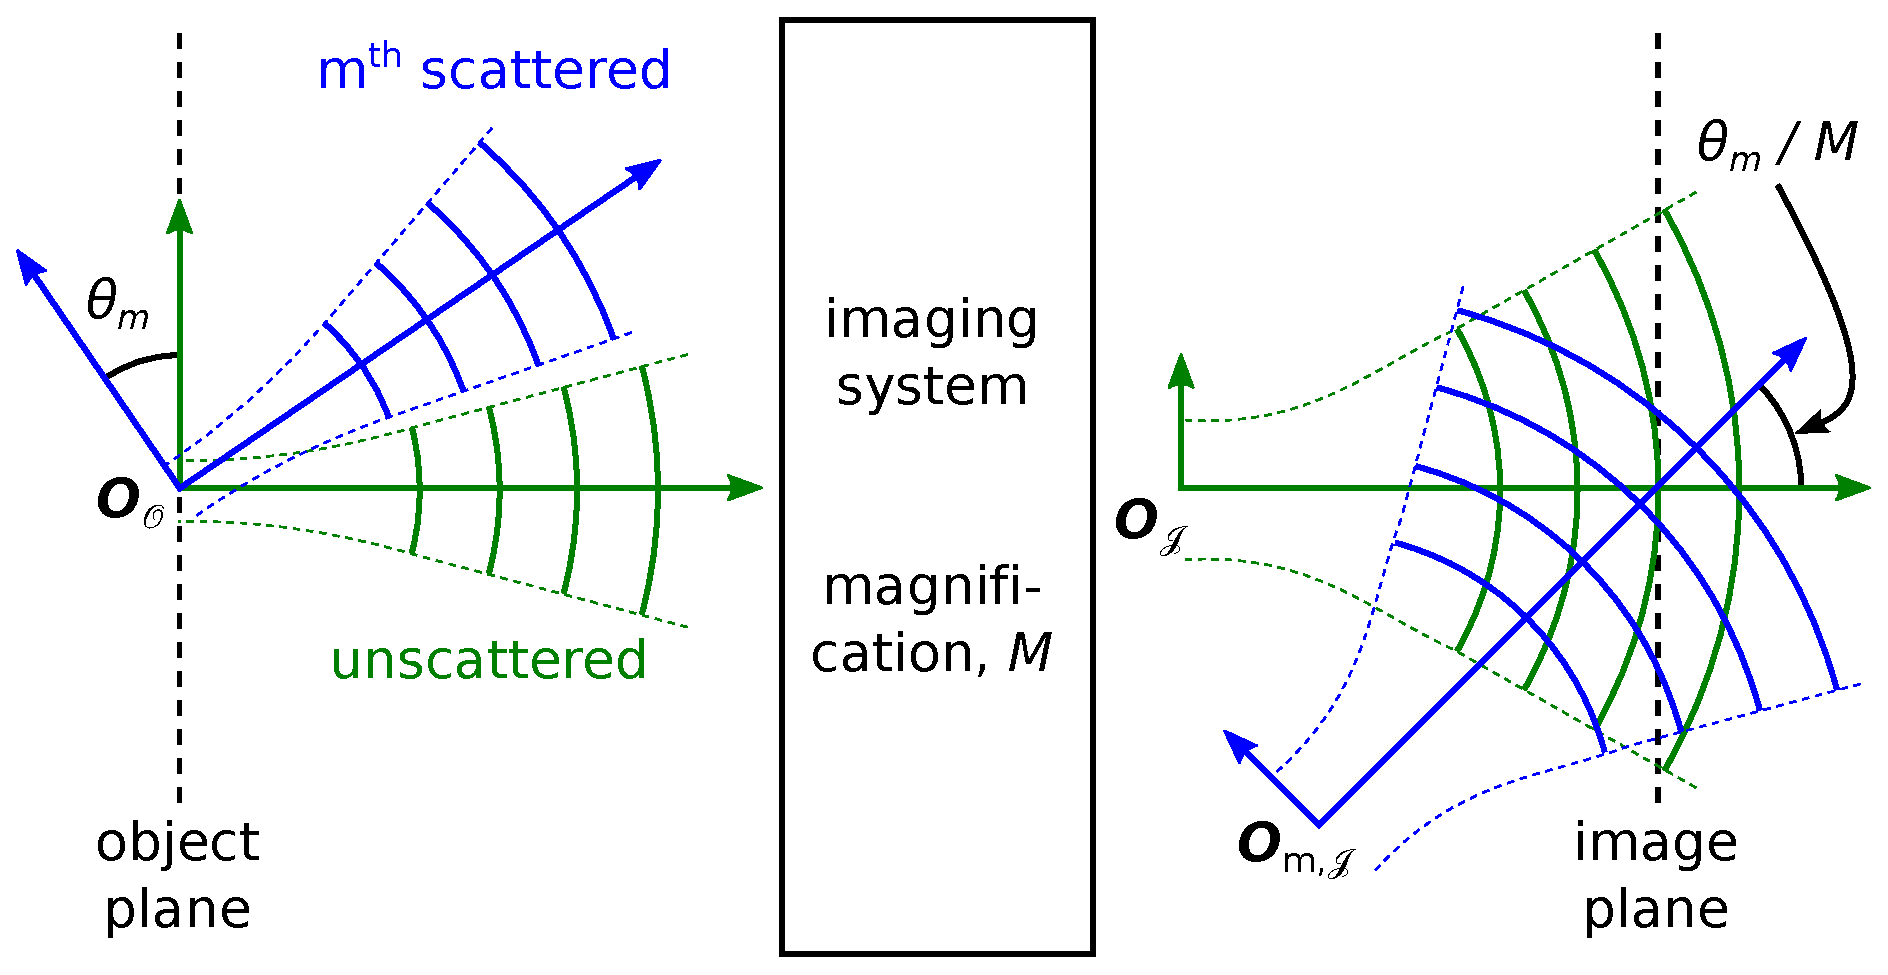
\includegraphics[width = \textwidth]{%
    Appendices/ImagingSystems/figs/imaging_geometry.eps}
  \caption[Imaging geometry]{%
    Beam geometries in an imaging system with magnification $M$.
    Beam scattering occurs in the object plane at the probe beam's waist.
    Thus, the $m$\ts{th} scattered beam
    shares the origin $\vect{O}_{\object}$ with the unscattered beam but
    is angularly separated by $\theta_m$.
    The imaging system redirects all beams emanating from $\vect{O}_{\object}$
    to intersect at angle $\theta_m / M$ in the image plane.
    In general, the image plane does \emph{not} sit at a beam waist
    such that the post-imaging-system beam waists
    of the scattered and unscattered beams do not coincide,
    i.e.\ $\vect{O}_{\image} \neq \vect{O}_{m,\image}$.}
\label{fig:ImagingSystems:imaging_geometry}
\end{figure}


\section{Gaussian-beam transformation in imaging systems}
\label{sec:ImagingSystems:imaging:Gaussian_beam_transformation}
In addition to manipulating the ray-like trajectory
of a Gaussian beam's symmetry axis,
an imaging system also alters
other important properties of an incident Gaussian beam.
A Gaussian beam is fully characterized by
its in-medium wavelength $\lambda_0 / N$,
its width $w(z_j)$, and
its radius of curvature $R(z_j)$
at a single location $z_j$.
These parameters can be conveniently combined
to define the so-called complex beam parameter $q$
\cite[Sec.~17.1]{siegman_lasers}
\begin{equation}
  \frac{1}{q}
  \equiv
  \frac{1}{R}
  -
  i \left( \frac{\lambda_0}{N \pi w^2} \right).
  \label{eq:ImagingSystems:complex_beam_parameter_inverse}
\end{equation}
Referencing the Gaussian-beam width
(\ref{eq:InterferometricMethods:Gaussian_beam_width}) and
the Gaussian-beam radius of curvature
(\ref{eq:InterferometricMethods:Gaussian_beam_radius_of_curvature}),
the complex beam parameter can be rewritten as
\begin{equation}
  q = z + i z_R,
  \label{eq:ImagingSystems:complex_beam_parameter}
\end{equation}
where $z$ is the axial distance from the beam waist and
$z_R$ is the Rayleigh range (\ref{eq:InterferometricMethods:Rayleigh_range}).
The Gaussian beam can then be propagated from point $j$ to point $j + 1$ via
\begin{equation}
  q_{j+1}
  =
  \frac{A q_j + B}{C q_j + D},
  \label{eq:ImagingSystems:complex_beam_parameter_propagation}
\end{equation}
where, amazingly, $A$, $B$, $C$, and $D$
are equal to the corresponding values
of the $ABCD$ ray matrix from geometric optics
\cite[Sec.~20.2]{siegman_lasers} \cite{tovar_generalized_beam_matrices_IV}.
The beam's transverse and angular displacements
relative to the lab-frame optical axis
are similarly governed by the so-called ``$S$-parameter transformation''
\cite{tovar_generalized_beam_matrices_IV}.
It is important to note that the complex beam parameter and its evolution
are \emph{independent} of the beam's transverse and angular displacements
from the lab-frame optical axis
(assuming such displacements do not violate the paraxial limit, of course);
that is, a scattered beam's width and radius of curvature
evolve identically to those of the unscattered beam.

The properties of the image-plane beams are easily determined.
Using the ray matrix of an imaging system from
(\ref{eq:ImagingSystems:ABCD_imaging}),
the image-plane complex beam parameter $q_{\image}$ is given as
\begin{equation}
  q_{\image}
  =
  \frac{M q_{\object}}{C q_{\object} + (1 / M)},
  \label{eq:ImagingSystems:complex_beam_parameter_image_plane}
\end{equation}
where $q_{\object}$ is the object-plane complex beam parameter,
and $M$ and $C$ are both real.
Note that the post-imaging-system beam waists
do \emph{not} necessarily sit at the image plane,
in which case the beams' native coordinate systems
are necessarily \emph{displaced} from each other
(i.e.\ $\vect{O}_{\image} \neq \vect{O}_{m,\image}$,
as indicated in Fig.~\ref{fig:ImagingSystems:imaging_geometry}).
Examining the image-plane complex beam parameter
(\ref{eq:ImagingSystems:complex_beam_parameter_image_plane})
it is easy to see that the beam waists will not sit at the image plane
when $|C q_{\object}| \gg 1 / M$ such that
$z_{\image} = \text{Re}(q_{\image}) \approx M / C \neq 0$.

As the native coordinate systems of
the unscattered beam and the $m$\ts{th} scattered beam
do not align in the image plane,
it will be convenient to determine the relevant coordinate transformation.
The transformation is derived for the most general case
in which the beam waists do not sit at the image plane
(i.e.\ $\vect{O}_{\image} \neq \vect{O}_{m,\image}$,
as indicated in Fig.~\ref{fig:ImagingSystems:imaging_geometry}).
The coordinate transformation is simply a series of translations and rotations
\begin{equation}
  \vect{r}_{m, \image}
  =
  \left[ \vect{R}(\theta_m / M) \right]
  \left[ \vect{r}_{\image} - z_{\image} \hat{\vect{z}} \right]
  +
  z_{\image} \hat{\vect{z}},
  \label{eq:ImagingSystems:coordinate_transformation_imaging_plane_compact}
\end{equation}
where
\begin{equation}
  \vect{R}(\theta)
  =
  \begin{pmatrix}
    \cos\theta & 0 & -\sin\theta
    \\
    0          & 1 & 0
    \\
    \sin\theta & 0 & \cos\theta
  \end{pmatrix}
  \label{eq:ImagingSystems:rotation_matrix}
\end{equation}
is the rotation matrix
that rotates the $(x, z)$-plane about the $y$-axis by angle $\theta$.
Explicitly, the image-plane coordinate transformation
(\ref{eq:ImagingSystems:coordinate_transformation_imaging_plane_compact}) is
\begin{equation}
  \begin{pmatrix}
    x_{m, \image}
    \\
    y_{m, \image}
    \\
    z_{m, \image}
  \end{pmatrix}
  =
  \begin{pmatrix}
    x_{\image} \cos\left( \frac{\theta_m}{M} \right)
    \\
    y_{\image}
    \\
    z_{\image} + x_{\image} \sin\left( \frac{\theta_m}{M} \right)
  \end{pmatrix}
  \approx
  \begin{pmatrix}
    x_{\image}
    \\
    y_{\image}
    \\
    z_{\image} + x_{\image} \left( \frac{\theta_m}{M} \right)
  \end{pmatrix},
  \label{eq:ImagingSystems:coordinate_transformation_imaging_plane}
\end{equation}
where the approximation is valid to first order in $\theta_m / M$.

Imagine now that the detector is located an axial distance $\delta z_{\image}$
downstream of the image plane
(i.e.\ $z_{\text{det}} = z_{\image} + \delta z_{\image}$ such that
positive $\delta z_{\image}$ implies that
the detector is downstream of the image plane, and
negative $\delta z_{\image}$ implies that
the detector is upstream of the image plane).
Coordinate transformation
(\ref{eq:ImagingSystems:coordinate_transformation_imaging_plane_compact})
then readily generalizes to
\begin{equation}
  \vect{r}_{m, \text{det}}
  =
  \left[ \vect{R}(\theta_m / M) \right]
  \left[ \vect{r}_{\text{det}} - z_{\image} \hat{\vect{z}} \right]
  +
  z_{\image} \hat{\vect{z}},
  \label{eq:ImagingSystems:coordinate_transformation_detector_plane_compact}
\end{equation}
where
$\vect{r}_{\text{det}}
=
\vect{r}_{\image} + (\delta z_{\image}) \hat{\vect{z}}$
specifies the detector-plane coordinates of the unscattered beam and
$\vect{r}_{m, \text{det}}$ specifies the detector-plane coordinates
of the $m\ts{th}$ scattered beam.
Explicitly, the detector-plane coordinate transformation
(\ref{eq:ImagingSystems:coordinate_transformation_detector_plane_compact}) is
\begin{align}
  \begin{pmatrix}
    x_{m, \text{det}}
    \\
    y_{m, \text{det}}
    \\
    z_{m, \text{det}}
  \end{pmatrix}
  &=
  \begin{pmatrix}
    x_{\text{det}} \cos\left( \frac{\theta_m}{M} \right)
    -
    \delta z_{\image} \sin\left( \frac{\theta_m}{M} \right)
    \\
    y_{\text{det}}
    \\
    z_{\image}
    +
    \delta z_{\image} \cos\left( \frac{\theta_m}{M} \right)
    +
    x_{\image} \sin\left( \frac{\theta_m}{M} \right)
  \end{pmatrix}
  \notag \\
  &\approx
  \vect{r}_{\text{det}}
  +
  \frac{\theta_m}{M}
  \begin{pmatrix}
    -\delta z_{\image}
    \\
    0
    \\
    x_{\text{det}}
  \end{pmatrix}
  -
  \frac{1}{2}
  {\left( \frac{\theta_m}{M} \right)}^2
  \begin{pmatrix}
    x_{\text{det}}
    \\
    0
    \\
    \delta z_{\image}
  \end{pmatrix},
  \label{eq:ImagingSystems:coordinate_transformation_detector_plane}
\end{align}
where the approximation is valid to second order in $\theta_m / M$.
As discussed in
Section~\ref{sec:DesignConsiderations:geometric:depth_of_focus},
second-order effects can become significant
when the detector is displaced from the image plane
(i.e.\ when $\delta z_{\image} \neq 0$).


\bibliographystyle{plainurl}
\bibliography{references}
%
\chapter{Some identities for the PCI wavenumber response}
\label{app:PCIResponseIdentities}


\section{Phase factor in the beam's near field}
The effect of wavenumber-dependent manipulation $T(k_x)$
on the $m$\ts{th} scattered beam is given by
the phase factor $\mathcal{P}(m, k, x)$ as defined in
(\ref{eq:InterferometricMethods:mth_diffracted_beam_kx_filtered_phase_factor}),
which is repeated here for completeness
\begin{equation}
  \begin{aligned}
    \mathcal{P}(m, k, x)
    &=
    \frac{1}{2 \pi}
    \int dx' \,
    \exp\left[ \frac{-x'^2}{w(z)^2} \right]
    \exp\left\{%
      i \left[%
        m k x'
        +
        \frac{k_0 x'^2}{2 R(z)}
      \right]
    \right\}
    \\
    &\qquad \times
    \int dk_x' \,
    T(k_x')
    e^{i k_x' (x_m - x')}
  \end{aligned}
  \label{eq:PCIResponseIdentities:mth_diffracted_beam_kx_filtered_phase_factor_full}
\end{equation}
The integrals are over the full domain of $x'$ and $k_x'$, but
note that contributions to the integral
from regions outside of $|x'| \lesssim w(z)$
are suppressed by the Gaussian envelope such that
the maximum value of the curvature-induced phase factor obeys
\begin{equation}
  \left[ \frac{k_0 x'^2}{2 R(z)} \right]_{\text{max}}
  \sim
  \frac{k_0 [w(z)]^2}{2 R(z)}
  \label{eq:PCIResponseIdentities:curvature_phase_factor_constraint_general}
\end{equation}
Now, in the beam's near field
($z \ll z_R$, which is often experimentally relevant),
the beam's waist and radius of curvature are
\begin{align}
  w(z) &\approx w_0
  \\
  R(z) &\approx \frac{z_R^2}{z}
\end{align}
as can be easily verified by examining the definitions in
(\ref{eq:InterferometricMethods:Gaussian_beam_width}) and
(\ref{eq:InterferometricMethods:Gaussian_beam_radius_of_curvature}),
respectively.
Thus,
(\ref{eq:PCIResponseIdentities:curvature_phase_factor_constraint_general})
becomes
\begin{align}
  \left[ \frac{k_0 x'^2}{2 R(z)} \right]_{\text{max}}
  &\sim
  \frac{k_0 [w(z)]^2}{2 R(z)}
  \notag \\
  &\approx
  \frac{k_0 w_0^2}{2 (z / z_R)}
  \notag \\
  &= \frac{z}{z_R}
  \notag \\
  &\ll 1
  \label{eq:PCIResponseIdentities:curvature_phase_factor_constraint_near_field}
\end{align}
where $z / z_R \ll 1$ follows from the near-field assumption.
Thus, in the beam's near field,
the curvature-induced phase factor is negligible, and
$\mathcal{P}(m, k, x)$ reduces to
\begin{equation}
  \begin{aligned}
    \mathcal{P}(m, k, x)
    &=
    \frac{1}{2 \pi}
    \int dx' \,
    e^{-\left[ x' / w(z) \right]^2}
    e^{i m k x'}
    \\
    &\qquad \times
    \int dk_x' \,
    T(k_x')
    e^{i k_x' (x_m - x')}
  \end{aligned}
  \label{eq:PCIResponseIdentities:mth_diffracted_beam_kx_filtered_phase_factor_near_field}
\end{equation}
This near-field assumption will be implicit
in the remainder of the discussion about PCI.


\section{The PCI phase factor}
The transfer function of the PCI phase plate can be described as
\begin{equation}
  \begin{aligned}
    T(k_x)
    &=
    i \sqrt{\eta} \, H(k_g - |k_x|)
    \\
    &\quad +
    H(|k_x| - k_g)
    H(k_D - |k_x|)
  \end{aligned}
  \label{eq:PCIResponseIdentities:phase_plate_transfer_function}
\end{equation}
where $H(x)$ is the Heaviside step function defined as
\begin{equation}
  H(x)
  =
  \begin{cases}
    0, \quad &x < 0 \\
    1, \quad &x \geq 0
  \end{cases}
  \label{eq:PCIResponseIdentities:Heaviside_step_function}
\end{equation}
$\eta$ is the reflectivity of the phase-plate groove, and
$k_g$ and $k_D$ are the low-$k$ and high-$k$ cutoffs of the phase plate
as defined in
(\ref{eq:InterferometricMethods:pci_kmin_engineering}) and
(\ref{eq:InterferometricMethods:pci_kmax_engineering}), respectively.
Note that the first term on the right-hand side of
(\ref{eq:PCIResponseIdentities:phase_plate_transfer_function})
corresponds to reflection from the phase-plate groove, while
the second term corresponds to reflection
from the non-grooved portion of the phase plate (i.e.\ the ``face'').
Thus, the PCI phase factor $\mathcal{P}(m, k, x)$ is
\begin{equation}
  \begin{aligned}
    \mathcal{P}(m, k, x)
    &=
    \frac{1}{2 \pi}
    \int dx' \,
    e^{-\left[ x' / w(z) \right]^2}
    e^{i m k x'}
    \\
    &\begin{aligned}
      \quad
      \times
      \Biggl\{%
        &\int_{-k_D}^{-k_g} dk_x' \,
        e^{i k_x' (x_m - x')}
        \\
        &+
        i \sqrt{\eta}
        \int_{-k_g}^{k_g} dk_x' \,
        e^{i k_x' (x_m - x')}
        \\
        &+
        \int_{k_g}^{k_D} dk_x' \,
        e^{i k_x' (x_m - x')}
      \Biggr\}
    \end{aligned}
  \end{aligned}
  \label{eq:PCIResponseIdentities:mth_diffracted_beam_kx_filtered_phase_factor_near_field_integrals}
\end{equation}


\section{Some useful integrals for evaluation of $\mathcal{P}(m, k, x)$}


\subsection{Finite-domain inverse Fourier transforms of unity}
Note that
\begin{equation}
  \int_{k_1}^{k_2} dk_x
  e^{i k_x x}
  =
  \frac{e^{i k_2 x} - e^{i k_1 x}}{ix}
\end{equation}
Now, if $k_1 = -k_2$, this simplifies to
\begin{equation}
  \int_{-k_2}^{k_2} dk_x
  e^{i k_x x}
  =
  2 k_2 \sinc \left( \frac{k_2 x}{\pi} \right)
  \label{eq:PCIResponseIdentities:finite_domain_inverse_FT_groove}
\end{equation}
where
\begin{equation}
  \sinc(x) = \frac{\sin(\pi x)}{\pi x}
  \label{eq:PCIResponseIdentities:normalized_sinc}
\end{equation}
is the normalized sinc function;
note that sinc is an \emph{even} function.
Finally, note that
\begin{align}
  \int_{-k_2}^{-k_1}
  &dk_x
  e^{i k_x x}
  +
  \int_{k_1}^{k_2} dk_x
  e^{i k_x x}
  \notag \\
  &=
  \int_{-k_2}^{k_2} dk_x
  e^{i k_x x}
  -
  \int_{-k_1}^{k_1} dk_x
  e^{i k_x x}
  \notag \\
  &=
  2 k_2 \sinc \left( \frac{k_2 x}{\pi} \right)
  -
  2 k_1 \sinc \left( \frac{k_1 x}{\pi} \right)
  \label{eq:PCIResponseIdentities:finite_domain_inverse_FT_face}
\end{align}
Using (\ref{eq:PCIResponseIdentities:finite_domain_inverse_FT_groove}) and
(\ref{eq:PCIResponseIdentities:finite_domain_inverse_FT_face}),
it is easy to see that
(\ref{eq:PCIResponseIdentities:mth_diffracted_beam_kx_filtered_phase_factor_near_field_integrals})
becomes
\begin{equation}
  \begin{aligned}
    \mathcal{P}(m, k, x)
    &=
    \frac{1}{\pi}
    \int dx' \,
    e^{-\left[ x' / w(z) \right]^2}
    e^{i m k x'}
    \\
    &\begin{aligned}
      \quad
      \times
      \Biggl\{%
        &k_D \sinc\left[ \frac{k_D}{\pi} (x' - x_m) \right]
        \\
        &-
        k_g \sinc\left[ \frac{k_g}{\pi} (x' - x_m) \right]
        \\
        &+
        i \sqrt{\eta}
        k_g \sinc\left[ \frac{k_g}{\pi} (x' - x_m) \right]
      \Biggr\}
    \end{aligned}
  \end{aligned}
  \label{eq:PCIResponseIdentities:mth_diffracted_beam_kx_filtered_phase_factor_near_field_sincs}
\end{equation}


\subsection{Integral of offset sinc with complex-Gaussian weighting}
Note that
(\ref{eq:PCIResponseIdentities:mth_diffracted_beam_kx_filtered_phase_factor_near_field_sincs})
consists of several integrals of the form
\begin{equation}
  I
  \equiv
  \frac{b}{\pi}
  \int dx \,
  e^{-a x^2}
  e^{i c x}
  \sinc\left[ \frac{b}{\pi} (x - x_0) \right]
  \label{eq:PCIResponseIdentities:I_x0_abc_definition}
\end{equation}
where $a > 0$ and $x_0$, $b$, and $c$ are real.
While daunting, the integral can be evaluated ``analytically''
in terms of complex error functions as follows
\begin{align}
  I
  &=
  \frac{b}{\pi}
  \int dx \,
  e^{-a x^2}
  e^{i c x}
  \sinc\left[ \frac{b}{\pi} (x - x_0) \right]
  \notag \\
  &=
  \frac{1}{\pi}
  \int dx \,
  e^{-a x^2}
  e^{i c x}
  \cdot
  \frac{\sin[b (x - x_0)]}{x - x_0}
  \notag \\
  &=
  \frac{1}{\pi}
  \int_{0}^{b} d\beta
  \int dx \,
  e^{-a x^2}
  e^{i c x}
  \cos[\beta (x - x_0)]
  \notag \\
  &=
  \frac{1}{2 \pi}
  \int_{0}^{b} d\beta
  \int dx \,
  e^{-a x^2}
  e^{i c x}
  \left[%
    e^{i \beta (x - x_0)}
    +
    e^{-i \beta (x - x_0)}
  \right]
  \notag \\
  &\begin{aligned}
    &=
    \frac{1}{2 \pi}
    \int_{0}^{b} d\beta
    \int dx \,
    e^{-a x^2}
    e^{i [(\beta + c) x - \beta x_0]}
    \\
    &\quad+
    \frac{1}{2 \pi}
    \int_{0}^{b} d\beta
    \int dx \,
    e^{-a x^2}
    e^{i [-(\beta - c) x + \beta x_0]}
  \end{aligned}
  \notag \\
  &\begin{aligned}
    &=
    \frac{1}{2 \pi}
    \int_{0}^{b} d\beta
    \int dx \,
    e^{-a x^2}
    e^{i [(\beta + c) x - \beta x_0]}
    \\
    &\quad-
    \frac{1}{2 \pi}
    \int_{0}^{-b} d\beta'
    \int dx \,
    e^{-a x^2}
    e^{i [(\beta' + c) x - \beta' x_0]}
  \end{aligned}
  \notag \\
  &=
  \frac{1}{2 \pi}
  \int_{-b}^{b} d\beta
  \int dx \,
  e^{-a x^2}
  e^{i [(\beta + c) x - \beta x_0]}
  \notag \\
  &=
  \frac{1}{2 \pi}
  \int_{-b}^{b} d\beta \,
  e^{-(\beta + c)^2 / 4 a}
  e^{-i \beta x_0}
  \int dx \,
  e^{-a [x - i (\beta + c) / 2a]^2}
  \notag \\
  &=
  \frac{1}{2 \sqrt{\pi a}}
  \int_{-b}^{b} d\beta \,
  e^{-(\beta + c)^2 / 4 a}
  e^{-i \beta x_0}
  \notag \\
  &=
  \frac{1}{2 \sqrt{\pi a}}
  e^{i c x_0}
  \int_{c - b}^{c + b} d\beta' \,
  e^{-\beta'^2 / 4 a}
  e^{-i \beta' x_0}
  \notag \\
  &=
  \frac{1}{2 \sqrt{\pi a}}
  e^{-a x_0^2}
  e^{i c x_0}
  \int_{c - b}^{c + b} d\beta' \,
  e^{-(\beta' + i 2 a x_0)^2 / 4 a}
  \notag \\
  &=
  \frac{1}{\sqrt{\pi}}
  e^{-a x_0^2}
  e^{i c x_0}
  \int_{u(c, - b)}^{u(c, b)} du \,
  e^{-u^2}
  \notag \\
  &=
  \frac{1}{2}
  e^{-a x_0^2}
  e^{i c x_0}
  \left\{
    \erf[u(c, b)]
    -
    \erf[u(c, - b)]
  \right\}
  \label{eq:PCIResponseIdentities:I_x0_abc_evaluated}
\end{align}
where the error function is defined for complex argument $z$ as
\begin{equation}
  \erf(z)
  =
  \frac{2}{\sqrt{\pi}}
  \int_0^z e^{-t^2} dt
  \label{eq:PCIResponseIdentities:error_function}
\end{equation}
and
\begin{equation}
  u(c, b) = \frac{1}{2 \sqrt{a}} [(c + b) + i 2 a x_0]
\end{equation}

Now, substituting the appropriate values
into (\ref{eq:PCIResponseIdentities:I_x0_abc_evaluated})
\begin{equation}
  x_0 \equiv x_m,
  \qquad
  a \equiv \frac{1}{w(z)^2},
  \qquad
  b \equiv k_j,
  \qquad
  c \equiv mk
  \notag
\end{equation}
yields
\begin{equation}
  I
  =
  \frac{1}{2}
  e^{-[x_m / w(z)]^2}
  e^{i m k x_m}
  \mathcal{D}(m, k_j, k, x)
  \label{eq:PCIResponseIdentities:I_x0_abc_evaluated_lab_parameters}
\end{equation}
where the difference function $\mathcal{D}$ is defined as
\begin{equation}
  \mathcal{D}(m, k_j, k, x)
  =
  \erf[u(m, k_j, k, x)]
  -
  \erf[u(m, -k_j, k, x)]
  \label{eq:PCIResponseIdentities:difference_function}
\end{equation}
and
\begin{equation}
  u(m, k_j, k, x)
  =
  \frac{w(z)}{2}
  \left[%
    (m k + k_j)
    +
    i \frac{2 x_m}{w(z)^2}
  \right]
  \label{eq:PCIResponseIdentities:u}
\end{equation}
With these definitions
the PCI phase factor from
(\ref{eq:PCIResponseIdentities:mth_diffracted_beam_kx_filtered_phase_factor_near_field_sincs})
readily reduces to
\begin{equation}
  \begin{aligned}
    \mathcal{P}(m, k, x)
    &=
    \frac{1}{2}
    e^{-[x_m / w(z)]^2}
    e^{i m k x_m}
    \\
    &\quad\times
    \left[%
       \mathcal{D}(m, k_D, k, x)
       +
       (i \sqrt{\eta} - 1)
       \mathcal{D}(m, k_g, k, x)
    \right]
  \end{aligned}
  \label{eq:PCIResponseIdentities:mth_diffracted_beam_kx_filtered_phase_factor_near_field_difference_functions}
\end{equation}


\section{Symmetries and degeneracies in the image plane}
The plasma midplane sits at the object plane
of a magnification-$M$ imaging system.
The probe beam's waist also nominally sits at this object plane,
with a 1/e $E$ radius of $w_{0,\object}$, and
the plasma dimensions are far smaller than the corresponding Rayleigh length
such that throughout the plasma volume
\begin{equation}
  w(z) \approx w_{0,\object}
\end{equation}
As discussed in
Section~\ref{sec:InterferometricMethods:imaging:Gaussian_beam_transformation},
the waist of the imaged beam
does \emph{not} necessarily occur at the image plane.
However, the derivation of
(\ref{eq:PCIResponseIdentities:mth_diffracted_beam_kx_filtered_phase_factor_near_field})
required assuming that the beam was well within its Rayleigh range
(i.e.\ $|z_{\image}| \ll z_{R,\image}$).
Thus, valid application of any of the above derived results to the image plane
requires that the image plane and the waist of the imaged beam
approximately overlap such that
\begin{equation}
  w(z_{\image}) \approx w_{0,\image} \approx M w_{0,\object}
  \label{eq:PCIResponseIdentities:criterion_on_imaged_beam_radius}
\end{equation}
where $w_{0,\image}$ is the 1/e $E$ radius of the imaged beam at its waist.

Further, according to the image-plane coordinate transformation in
(\ref{eq:InterferometricMethods:coordinate_transformation_imaging_plane}),
\begin{equation}
  x_{m,\image} = x_{\image}
\end{equation}
to first order in $k / k_0$; that is,
$x_{m,\image}$ is \emph{independent} of $m$ in the image plane.
This leads to several useful symmetries in the image plane.


\subsection{Properties of $u$ in the image plane}
The complex-valued function $u$ is defined in
(\ref{eq:PCIResponseIdentities:u}).
Note that $u$ is anti-Hermitian
with respect to $m$ and $k_{j,\image}$
\begin{align}
  u(-m, -k_{j,\image}, k_{\image}, x_{\image})
  &=
  \frac{w(z_{\image})}{2}
  \left[%
    (-m k_{\image} - k_{j,\image})
    +
    i \frac{2 x_{m,\image}}{w(z_{\image})^2}
  \right]
  \notag \\
  &=
  \frac{w(z_{\image})}{2}
  \left[%
    -(m k_{\image} + k_{j,\image})
    +
    i \frac{2 x_{\image}}{w(z_{\image})^2}
  \right]
  \notag \\
  &=
  \frac{-w(z_{\image})}{2}
  \left[%
    (m k_{\image} + k_{j,\image})
    -
    i \frac{2 x_{\image}}{w(z_{\image})^2}
  \right]
  \notag \\
  &=
  \frac{-w(z_{\image})}{2}
  \left[%
    (m k_{\image} + k_{j,\image})
    +
    i \frac{2 x_{\image}}{w(z_{\image})^2}
  \right]^*
  \notag \\
  &=
  -[u(m, k_{j,\image}, k_{\image}, x_{\image})]^*
\end{align}
where $z^*$ indicates the complex conjugate of $z$.
Further, referencing
(\ref{eq:PCIResponseIdentities:criterion_on_imaged_beam_radius}),
note that
\begin{align}
  u(m, k_{j,\image}, k_{\image}, x_{\image})
  &=
  \frac{w(z_{\image})}{2}
  \left[%
    (m k_{\image} + k_{j,\image})
    +
    i \frac{2 x_{\image}}{w(z_{\image})^2}
  \right]
  \notag \\
  &\approx
  \frac{M w_{0,\object}}{2}
  \left[%
    \left(\frac{m k}{M} + \frac{k_j}{M}\right)
    +
    i \frac{2 M x_{\object}}{(M w_{0,\object})^2}
  \right]
  \notag \\
  &=
  \frac{w_{0,\object}}{2}
  \left[%
    \left(m k + k_j \right)
    +
    i \frac{2 x_{\object}}{w_{0,\object}}
  \right]
  \notag \\
  &=
  u(m, k_{j,\object}, k, x_{\object})
\end{align}
that is,
$u(m, k_{j,\image}, k_{\image}, x_{\image})$ and
$u(m, k_{j,\object}, k, x_{\object})$ are geometrically \emph{similar},
as is expected in an imaging system.


\subsection{Properties of the error function}
The error function has two useful properties
that will be exploited shortly.
First, the error function is \emph{odd}
\begin{equation}
  \erf(-z) = - \erf(z)
  \label{eq:PCIResponseIdentities:error_function_is_odd}
\end{equation}
as is easily determined by inspection.
Second, the error function \emph{commutes} with complex conjugation
\begin{equation}
  \erf(z^*) = [\erf(z)]^*
  \label{eq:PCIResponseIdentities:error_function_commutativity}
\end{equation}
where $z^*$ is the complex conjugate of $z$.


\subsection{Properties of $\mathcal{D}$ in the image plane}
The complex-valued difference function $\mathcal{D}$ is defined in
(\ref{eq:PCIResponseIdentities:difference_function}).
Note that $\mathcal{D}$ is Hermitian with respect to $m$
\begin{align}
  &\begin{aligned}
    \mathcal{D}(-m, k_{j,\image}, k_{\image}, x_{\image})
    &=
    \erf[u(-m, k_{j,\image}, k_{\image}, x_{\image})]
    \\
    &\quad
    -
    \erf[u(-m, -k_{j,\image}, k_{\image}, x_{\image})]
  \end{aligned}
  \notag \\
  &\begin{aligned}
    \phantom{\mathcal{D}(-m, k_{j,\image}, k_{\image}, x_{\image})}
    &=
    \erf\{-[u(m, -k_{j,\image}, k_{\image}, x_{\image})]^*\}
    \\
    &\quad
    -
    \erf\{-[u(m, k_{j,\image}, k_{\image}, x_{\image})]^*\}
  \end{aligned}
  \notag \\
  &\begin{aligned}
    \phantom{\mathcal{D}(-m, k_{j,\image}, k_{\image}, x_{\image})}
    &=
    -\{\erf[u(m, -k_{j,\image}, k_{\image}, x_{\image})]\}^*
    \\
    &\quad
    +
    \{\erf[u(m, k_{j,\image}, k_{\image}, x_{\image})]\}^*
  \end{aligned}
  \notag \\
  &\begin{aligned}
    \phantom{\mathcal{D}(-m, k_{j,\image}, k_{\image}, x_{\image})}
    &=
    \{\erf[u(m, k_{j,\image}, k_{\image}, x_{\image})]
    \\
    &\quad
    -
    \erf[u(m, -k_{j,\image}, k_{\image}, x_{\image})]\}^*
  \end{aligned}
  \notag \\
  &\phantom{\mathcal{D}(-m, k_{j,\image}, k_{\image}, x_{\image})}
  =
  \mathcal{D}^*(m, k_{j,\image}, k_{\image}, x_{\image})
  \label{eq:PCIResponseIdentities:difference_function_symmetry}
\end{align}
The above symmetry relation also implies a degeneracy when $m = 0$; namely,
$\mathcal{D}(0, k_{j,\image}, k_{\image}, x_{\image})
=
\mathcal{D}^*(0, k_{j,\image}, k_{\image}, x_{\image})$,
which proves that
$\mathcal{D}(0, k_{j,\image}, k_{\image}, x_{\image})$
is purely \emph{real}.


\subsection{Properties of $\mathcal{P}$ in the image plane}
Using (\ref{eq:PCIResponseIdentities:difference_function_symmetry})
the PCI phase factor from
(\ref{eq:PCIResponseIdentities:mth_diffracted_beam_kx_filtered_phase_factor_near_field_difference_functions})
can be readily written as
\begin{equation}
  \begin{aligned}
    \mathcal{P}(m, k_{\image}, x_{\image})
    &=
    e^{-[x_{\image} / w(z_{\image})]^2}
    e^{i m k_{\image} x_{\image}}
    \\
    &\quad\times
    \left[%
      F(m, k_{\image}, x_{\image})
      +
      G(m, k_{\image}, x_{\image})
    \right]
  \end{aligned}
  \label{eq:PCIResponseIdentities:phase_factor_Hermitian_decomposed}
\end{equation}
where
\begin{align}
  F(m, k_{\image}, x_{\image})
  &=
  \frac{1}{2}
  \left[%
    \mathcal{D}(m, k_{D,\image}, k_{\image}, x_{\image})
    -
    \mathcal{D}(m, k_{g,\image}, k_{\image}, x_{\image})
  \right]
  \label{eq:PCIResponseIdentities:phase_factor_face}
  \\
  G(m, k_{\image}, x_{\image})
  &=
  \frac{i \sqrt{\eta}}{2} \, \mathcal{D}(m, k_{g,\image}, k_{\image}, x_{\image})
  \label{eq:PCIResponseIdentities:phase_factor_groove}
\end{align}
Here, the notation is mnemonic:
the non-grooved portion of the phase plate (i.e.\ the ``face'')
acts on the $m$\ts{th} scattered beam via $F$, while
the phase-plate groove acts on the $m$\ts{th} scattered beam via $G$.
Note that $F$ is Hermitian with respect to $m$
\begin{equation}
  F(-m, k_{\image}, x_{\image}) = F^*(m, k_{\image}, x_{\image})
  \label{eq:PCIResponseIdentities:mth_beam_interaction_with_face_hermitian}
\end{equation}
while $G$ is anti-Hermitian with respect to $m$
\begin{equation}
  G(-m, k_{\image}, x_{\image}) = -G^*(m, k_{\image}, x_{\image})
  \label{eq:PCIResponseIdentities:mth_beam_interaction_with_groove_antihermitian}
\end{equation}

Note that the above symmetries also imply a degeneracy when $m = 0$.
Specifically,
(\ref{eq:PCIResponseIdentities:mth_beam_interaction_with_face_hermitian})
states that $F(0, k_{\image}, x_{\image}) = F^*(0, k_{\image}, x_{\image})$;
that is, $F(0, k_{\image}, x_{\image})$ is purely \emph{real}
\begin{equation}
  F(0, k_{\image}, x_{\image}) = \real[F(0, k_{\image}, x_{\image})]
\end{equation}
Similarly,
(\ref{eq:PCIResponseIdentities:mth_beam_interaction_with_groove_antihermitian})
states that $G(0, k_{\image}, x_{\image}) = -G^*(0, k_{\image}, x_{\image})$;
that is, $G(0, k_{\image}, x_{\image})$ is purely \emph{imaginary}
\begin{equation}
  G(0, k_{\image}, x_{\image}) = i \cdot \imag[G(0, k_{\image}, x_{\image})]
\end{equation}

Another set of useful degeneracies occurs
when the fluctuation wavenumber vanishes (i.e.\ $k_{\image} = 0$).
Note that the $m$ and $k_{\image}$ dependence of $F$ and $G$
only appears as the \emph{product} $(m \cdot k_{\image})$.
Just as $m = 0$ at finite $k_{\image}$ yields $(m \cdot k_{\image}) = 0$,
$k_{\image} = 0$ at finite $m$ also gives $(m \cdot k_{\image}) = 0$;
thus,
\begin{align}
  F(m, k_{\image}=0, x_{\image}) &= F(m=0, k_{\image}, x_{\image})
  \label{eq:PCIResponseIdentities:mth_beam_interaction_with_face_for_wavenumber_0}
  \\
  G(m, k_{\image}=0, x_{\image}) &= G(m=0, k_{\image}, x_{\image})
  \label{eq:PCIResponseIdentities:mth_beam_interaction_with_groove_for_wavenumber_0}
\end{align}
Eqs.~(\ref{eq:PCIResponseIdentities:mth_beam_interaction_with_face_for_wavenumber_0})
and
(\ref{eq:PCIResponseIdentities:mth_beam_interaction_with_groove_for_wavenumber_0})
will be helpful in analytically showing
that the PCI response vanishes at $k_{\image} = 0$
(i.e.\ when the object-plane wavevector vanishes, $k = 0$).
%
\chapter{Oscillator phase noise}


\section{Motivation}
An oscillator with negligible amplitude variation is well-described by
\begin{equation}
  A(t) = A_0 e^{i [\omega_0 t + \phi(t)]},
\end{equation}
where $\phi(t)$ is a zero-mean, random process
whose temporal variation causes
the oscillator's instantaneous frequency
to wander about its nominal value $\nu_0 = \omega_0 / (2 \pi)$.
The oscillator's phase change between
times $t$ and $t + \tau_j$ is
\begin{equation}
  \arg[A(t + \tau_j) \cdot A^*(t)]
  =
  \omega_0 \tau_j + \phi(t + \tau_j) - \phi(t).
\end{equation}
In a perfect oscillator,
$\phi(t + \tau_j) = \phi(t)$ for all $t$ and $\tau_j$
such that the phase change is governed only by
the oscillator's nominal frequency $\omega_0 / (2 \pi)$ and
the time difference $\tau_j$.
Excursions from this ideal result in phase noise.

It is the goal of this appendix
to investigate the spectral properties
of an oscillator's phase noise.
Define the phase noise between times $t$ and $t + \tau_j$ to be
\begin{equation}
  \delta \phi(t, \tau_j)
  \equiv
  \phi(t + \tau_j) - \phi(t).
\end{equation}
This phase noise can be related to
the deviation in the oscillator's instantaneous frequency via
\begin{equation}
  \delta \phi(t, \tau_j)
  =
  2 \pi \int_{t}^{t + \tau_j} \delta \nu(t') dt'.
  \label{eq:OscillatorPhaseNoise:phase_noise_from_frequency_deviation}
\end{equation}
Whereas the phase noise $\delta \phi(t, \tau_j)$
depends on the externally imposed time difference $\tau_j$,
the oscillator's instantaneous frequency deviation $\delta \nu(t)$ does not
(i.e.\ it is an intrinsic property of the oscillator).


\section{Autospectral density of phase noise}
The two-sided autospectral density $S_{xx}(f)$
of a stationary random process $\{x_k(t)\}$ is simply
\begin{equation}
  S_{xx}(f) = \mathcal{F}[R_{xx}(\tau)](f),
\end{equation}
where $\mathcal{F}$ is the Fourier transform operator and
$R_{xx}(\tau)$ is the autocorrelation of $\{x_k(t)\}$
\cite{bendat_and_piersol}.
Below, the phase-noise autocorrelation
$R_{\delta\phi,\delta\phi}(\tau)$ is computed;
subsequently, the phase-noise autospectral density
$S_{\delta\phi,\delta\phi}(f)$ is computed
by Fourier transforming
$R_{\delta\phi,\delta\phi}(\tau)$.


\subsection{Autocorrelation of phase-noise}
The autocorrelation $R_{xx}(\tau)$
of a stationary random process $\{x_k(t)\}$ is defined as
\begin{equation}
  R_{xx}(\tau) = E\left[ x_k(t) x_k(t + \tau) \right],
\end{equation}
where $E$ is the expectation-value operator
that averages over all of the realizations in the ensemble $\{x_k(t)\}$
\cite{bendat_and_piersol}.
Thus, the phase noise
(\ref{eq:OscillatorPhaseNoise:phase_noise_from_frequency_deviation})
has an autocorrelation
\begin{align}
  R_{\delta\phi,\delta\phi}(\tau)
  &=
  E\left[ \delta\phi(t) \delta\phi(t + \tau) \right]
  \notag \\
  &=
  (2 \pi)^2
  \int_{t}^{t + \tau_j} dt'
  \int_{t + \tau}^{t + \tau + \tau_j} dt'' \,
  E[ \delta \nu(t') \delta \nu(t'') ],
  \label{eq:OscillatorPhaseNoise:phase_noise_autocorrelation_v1}
\end{align}
where the linearity of the expectation-value operator has been used
to bring $E$ into the integrand of the double integral.
Note that
$E[ \delta \nu(t') \delta \nu(t'') ]
=
R_{\delta\nu,\delta\nu}(t', t'')
=
R_{\delta\nu,\delta\nu}(t' - t'')$, where
the last equality follows from the fact that
the autocorrelation of a stationary process
cannot depend on the absolute times $t'$ and $t''$
\emph{except} through their difference $t' - t''$.
Thus, (\ref{eq:OscillatorPhaseNoise:phase_noise_autocorrelation_v1})
becomes
\begin{equation}
  R_{\delta\phi,\delta\phi}(\tau)
  =
  (2 \pi)^2
  \int_{t}^{t + \tau_j} dt'
  \int_{t + \tau}^{t + \tau + \tau_j} dt'' \,
  R_{\delta\nu,\delta\nu}(t' - t'').
  \label{eq:OscillatorPhaseNoise:phase_noise_autocorrelation_v2}
\end{equation}

Fortunately, a suitable change of variables
simplifies the expression for
$R_{\delta\phi,\delta\phi}(\tau)$ in
(\ref{eq:OscillatorPhaseNoise:phase_noise_autocorrelation_v2}).
To see this, define the integral
\begin{equation}
  I(g, \tau, \tau_j)
  \equiv
  \int_{a}^{a + \tau_j} dx
  \int_{a + \tau}^{a + \tau + \tau_j} dy \,
  g(x - y),
\end{equation}
and make the change of variables
\begin{equation}
  x = z + y,
  \label{eq:OscillatorPhaseNoise:change_of_variables}
\end{equation}
which transforms the integration domain as shown in
Fig.~\ref{fig:OscillatorPhaseNoise:integration_domains}.
Then, $I(g, \tau, \tau_j)$ becomes
\begin{align}
  I(g, \tau, \tau_j)
  &=
  \int_{- \tau_j - \tau}^{- \tau} dz \, g(z)
  \int_{a - z}^{a + \tau + \tau_j} dy
  +
  \int_{-\tau}^{\tau_j - \tau} dz \, g(z)
  \int_{a + \tau}^{a + \tau_j - z} dy
  \notag \\
  &=
  \int_{- \tau_j - \tau}^{- \tau} dz \,
  \left[ \tau_j + (z + \tau) \right]
  g(z)
  +
  \int_{-\tau}^{\tau_j - \tau} dz \,
  \left[ \tau_j - (z + \tau) \right]
  g(z)
  \notag \\
  &=
  \int_{-\tau_j}^{0} dz' \,
  \left[ \tau_j + z' \right]
  g(z' - \tau)
  +
  \int_{0}^{\tau_j} dz' \,
  \left[ \tau_j - z' \right]
  g(z' - \tau)
  \notag \\
  &=
  \int_{-\tau_j}^{\tau_j} dz' \,
  \left[ \tau_j - |z'| \right]
  g(z' - \tau)
  \label{eq:OscillatorPhaseNoise:integral_after_change_of_variables}
\end{align}
Substituting (\ref{eq:OscillatorPhaseNoise:integral_after_change_of_variables})
into (\ref{eq:OscillatorPhaseNoise:phase_noise_autocorrelation_v2})
with $g = R_{\delta\nu,\delta\nu}$ yields
\begin{equation}
  R_{\delta\phi,\delta\phi}(\tau)
  =
  (2 \pi)^2
  \int_{-\tau_j}^{\tau_j} dt' \,
  \left[ \tau_j - |t'| \right]
  R_{\delta\nu,\delta\nu}(t' - \tau).
  \label{eq:OscillatorPhaseNoise:phase_noise_autocorrelation_final}
\end{equation}

\begin{figure}
  \centering
  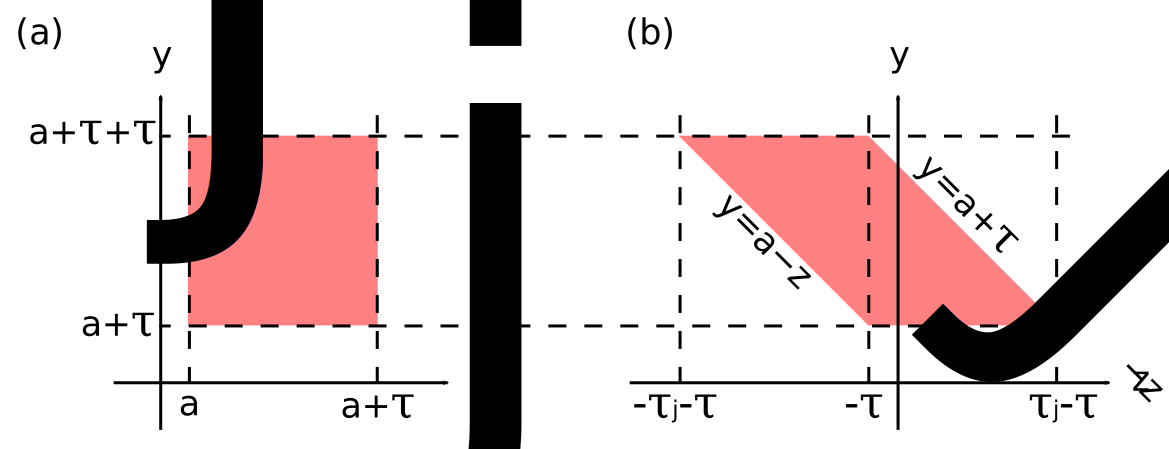
\includegraphics[width = \textwidth]{%
    Appendices/OscillatorPhaseNoise/figs/integration_domains.pdf}
  \caption[Integration domains]{
    Integration domains (a) before and (b) after
    the change of variables in
    (\ref{eq:OscillatorPhaseNoise:change_of_variables}).}
  \label{fig:OscillatorPhaseNoise:integration_domains}
\end{figure}


\bibliographystyle{plainurl}
\bibliography{references}
%
\chapter{Sound-wave characterization}
\label{app:SoundWaveCharacterization}
\begin{itemize}
  \item Sound-wave dispersion relation
\end{itemize}


\section{Hardware}
\label{sec:SoundWaveCharacterization:Hardware}
\subsection{Speaker}
\label{sec:SoundWaveCharacterization:Hardware:speaker}
\subsection{Calibrated microphone}
\label{sec:SoundWaveCharacterization:Hardware:microphone}
\subsection{Test stand}
\label{sec:SoundWaveCharacterization:Hardware:test_stand}


\section{Sound-wave measurements}
\label{sec:SoundWaveCharacterization:Measurements}
To lowest order, the speaker is cylindrically symmetric.
Thus, the sound waves are expected to have
axial, radial, and frequency dependencies.
Sections~\ref{sec:SoundWaveCharacterization:Measurements:amlitude} through
\ref{sec:SoundWaveCharacterization:Measurements:phasing}
summarize these measurements and their implications
for the sound-wave model developed in
Section~\ref{sec:SoundWaveCharacterization:Model}.


\subsection{On-axis amplitude}
\label{sec:SoundWaveCharacterization:Measurements:amlitude}
After centering the microphone on the speaker's symmetry axis,
the on-axis amplitude can be easily characterized by
varying both the frequency $f$ of the sound waves and
the microphone height $z$ above the speaker face.
The frequencies $f$ and heights $z$
are motivated by the parameters of the heterodyne interferometer
described in Chapter~\ref{ch:Implementation}.
Specifically, the interferometer spatial bandwidth
$|k| \leq \SI{5}{\per\centi\meter}$
from (\ref{eq:Implementation:kfsv_interferometer_design}) motivates
sound-wave measurements at frequencies
$f \lesssim \SI{30}{\kilo\hertz}$
(i.e.\ $|k| \lesssim \SI{5}{\per\centi\meter}$).
Further, to produce a robust interference signal
during sound-wave calibrations,
the speaker is placed very close
to the edge of the collimated probe beam,
which has 1/e $E$ radius $w_0 = \SI{3.4}{\centi\meter}$;
thus, sound-wave measurements are made at heights
spanning the probe-beam profile
$z
=
\{\SI{2.5}{\centi\meter}, \SI{5.5}{\centi\meter}, \SI{8.5}{\centi\meter}\}$.
The on-axis amplitude of the sound waves as a function of
wavenumber $k$ and height $z$ above the speaker face is shown in
Fig.~\ref{fig:SoundWaveCharacterization:tymphany_on_axis_amplitude}.
As expected, the on-axis amplitude decreases with
increasing distance $z$ from the speaker face.
Further, the on-axis amplitude has a complicated wavenumber dependence, but
it is relatively flat for
$\SI{1}{\per\centi\meter} \lesssim k \lesssim \SI{3.5}{\per\centi\meter}$.

\begin{figure}
  \centering
  \includegraphics[width = \textwidth]{%
    Appendices/SoundWaveCharacterization/figs/tymphany_on_axis_amplitude.pdf}
  \caption[On-axis amplitude of sound waves]{%
    On-axis amplitude of sound waves as a function of
    wavenumber $k$ and height $z$ above the speaker face.
    Note that the amplitude is specified
    as a \emph{peak-to-peak} value.
  }
\label{fig:SoundWaveCharacterization:tymphany_on_axis_amplitude}
\end{figure}


\subsection{Wavefront phasing}
\label{sec:SoundWaveCharacterization:Measurements:phasing}
Characterizing the sound-wave phasing is somewhat more involved
than characterizing the on-axis amplitude,
as it requires measurements at several radial positions $\rho$
for each frequency $f$ and microphone height $z$.
For this reason, the wavefront-phasing measurements
are more coarsely sampled in frequency $f$
than the on-axis amplitude measurements in
Section~\ref{sec:SoundWaveCharacterization:Measurements:amlitude}.
For a given frequency $f$ and height $z$,
the sound-wave phasing is measured by
tracking a point of constant phase in the microphone waveform
as the radial position $\rho$ is varied;
such tracking can be easily accomplished
by triggering the oscilloscope
with a copy of the waveform that is driving the speaker.
To begin the radial scan,
the microphone height $z$ is selected, and
the microphone is displaced from the speaker's symmetry axis
by a few centimeters.
Then, in $\SI{1}{\centi\meter}$ increments,
the microphone is moved radially inwards towards the center;
upon passing through the center,
the radial scan is continued in $\SI{1}{\centi\meter}$ increments
until the sound-wave amplitude becomes negligible.
Note that beginning the radial scan
with a small displacement from the symmetry axis
allows empirical identification of the symmetry-axis location
(by e.g.\ fitting the measured amplitude and/or phasing
and identifying the extremum that occurs at the symmetry axis).

\begin{figure}
  \centering
  \includegraphics[width = \textwidth]{%
    Appendices/SoundWaveCharacterization/figs/tymphany_wavefront_phasing.pdf}
  \caption[Wavefront phasing of sound waves]{%
    Wavefront phasing of sound waves.
    The symbols show the measured time delay $\tau$
    between the wavefront at height $z$ and radial displacement $\rho$ and
    the corresponding on-axis wavefront (i.e.\ same $z$ and $\rho = 0$),
    with each symbol shape corresponding to particular frequency.
    The traces correspond to the time delay
    (\ref{eq:SoundWaveCharacterization:time_delay})
    predicted for spherical waves.
    The close proximity of the measured points to the spherical-wave traces
    indicates that, to lowest order, the waves are approximately spherical
    over the spatial domain and frequencies probed.
  }
\label{fig:SoundWaveCharacterization:tymphany_wavefront_phasing}
\end{figure}

At sufficiently large distances,
the speaker will behave like a point source,
producing sound waves with spherical wavefronts.
This point-source approximation is taken as a reasonable
starting point for the investigation of the wavefront phasing.
If a sound wave is measured on axis at height $z$ above the speaker,
the corresponding wavefront will subsequently arrive
at position $r = (z^2 + \rho^2)$
delayed by a time $\tau$
\begin{equation}
  \tau = \frac{r - z}{c_s},
  \label{eq:SoundWaveCharacterization:time_delay}
\end{equation}
\graffito{\textcolor{red}{value for $c_s$}}
where $c_s$ is the sound speed.
Fig.~\ref{fig:SoundWaveCharacterization:tymphany_wavefront_phasing}
compares the measured time delay to
the time delay predicted for spherical waves
(\ref{eq:SoundWaveCharacterization:time_delay})
as a function of height $z$, radial position $\rho$, and frequency $f$.
Clearly, to lowest order, the waves are approximately spherical
over the spatial domain and frequencies probed.


\subsection{Spatial envelope}
\label{sec:SoundWaveCharacterization:Measurements:envelope}


\section{Sound-wave model}
\label{sec:SoundWaveCharacterization:Model}


\section{Perturbed index of refraction}
\label{sec:SoundWaveCharacterization:PerturbedIndexOfRefractiion}


\bibliographystyle{plainurl}
\bibliography{references}
%
\chapter{Spectral estimation}
\label{app:SpectralEstimation}
In contrast to deterministic processes,
random processes cannot be modeled via an explicit mathematical relationship.
Rather, random processes are characterized
in terms of probabilities and statistical properties.
Any given observation of a random process represents
only one of many possible observations;
each such observation is referred to as
a ``sample'' or a ``realization'' of the random process
and is denoted as $x_k(t)$.
The random process itself consists of
the ensemble of all of the potential observations
and is denoted as $\{x_k(t)\}$.
Random processes can be stationary or nonstationary.
The statistical properties of a stationary random process
do not vary in time.

The spectral tools discussed below
are all developed for analysis of stationary random processes.
Section~\ref{app:SpectralEstimation:NonParametric}
discusses non-parametric spectral-estimation techniques,
which find powerful and versatile application
in the analysis of uniformly and richly sampled data.
Section~\ref{app:SpectralEstimation:Parametric}
discuses parametric spectral-estimation techniques,
which find application
in the analysis of data with sharp spectral features,
particularly if the data is sparsely sampled.
Finally, Section~\ref{app:SpectralEstimation:2d_spectra}
discusses the hybrid non-parametric-in-time, parametric-in-space
technique used to estimate the PCI-measured
two-dimensional autospectral density function.


\section{Non-parametric techniques}
\label{app:SpectralEstimation:NonParametric}
Most of the discussion below is distilled from
the seminal work by Bendat and Piersol~\cite{bendat_and_piersol}, and
inquisitive readers are directed there
for a more extensive treatment of the subject.

The windowed, finite Fourier transform $X_k(f, T)$
of a continuous signal $x_k(t)$
sampled for $-T / 2 \leq t < T / 2$
is defined as
\begin{equation}
  X_k(f, T)
  =
  \int_{-T / 2}^{T / 2}
  dt \, [w(t) \cdot x_k(t)] e^{-i \, 2 \pi f t},
  \label{eq:SpectralEstimation:finite_Fourier_transform}
\end{equation}
where $w(t)$ is an arbitrary windowing function.
Typically, the selected windowing function smoothly tapers
as $|t| \rightarrow T / 2$
to minimize sidelobe leakage
that results from discontinuities at the start and end of the sample record.
Further, to prevent power loss, the windowing function
is also typically normalized such that
\begin{equation}
  \frac{1}{T} \int_{-T/2}^{T/2} dt \, [w(t)]^2 = 1.
\end{equation}
The normalized Hanning window is perhaps
the most commonly used windowing function, and
it is used uniformly throughout this work.

For real-valued, stationary random processes $\{x_k(t)\}$ and $\{y_k(t)\}$,
the one-sided \emph{cross-spectral density} function $G_{xy}(f)$ is defined as
\begin{equation}
  G_{xy}(f)
  \equiv
  \lim_{T \rightarrow \infty}
  \frac{2}{T} E \left[ X_k^*(f, T) Y_k(f, T) \right]
  \label{eq:SpectralEstimation:cross_spectral_density_defn}
\end{equation}
for $0 < f < \infty$;
$G_{xy}(f)$ is not defined for $f < 0$, and
it is reduced by a factor of two relative to
(\ref{eq:SpectralEstimation:cross_spectral_density_defn}) at $f = 0$
(the value of $G_{xy}(0)$ is of little relevance to this work).
Note that $E[\cdot]$ is the expectation value operator;
this operator averages over all of the realizations in the ensemble, and
its application ensures that
(\ref{eq:SpectralEstimation:cross_spectral_density_defn})
is a statistically consistent definition of the cross-spectral density
(that is, ensemble averaging is needed for $G_{xy}(f)$
to approach the true cross-spectral density
as $T \rightarrow \infty$). % see pgs. 127, 128 of Bendat & Piersol, 4th ed.
If, in addition to being stationary,
the random process is also \emph{ergodic},
the ensemble average can be replaced
with a time average of $X_k(f, T)$
over successive time slices.
If desired, these time slices may partially overlap.
Unless otherwise noted,
all of the ensemble averages in this work are computed
using this assumption of ergodicity, and
successive slices are selected to overlap by 50\%.

In general $G_{xy}(f)$ is a complex-valued function.
This can be made explicit by writing
\begin{equation}
  G_{xy}(f) = \left| G_{xy}(f) \right| e^{i \alpha_{xy}(f)},
  \label{eq:SpectralEstimation:cross_spectral_density_explicit_complex}
\end{equation}
where $\alpha_{xy}(f)$ is the \emph{cross phase}.
For the special case $\{x_k(t)\} = \{y_k(t)\}$,
$G_{xx}(f)$ is real-valued (i.e.\ $G_{xx}(f) = |G_{xx}(f)|$) and
is referred to as the one-sided \emph{autospectral density} function.

The degree of correlation between random processes
$\{x_k(t)\}$ and $\{y_k(t)\}$ can be easily quantified
with the corresponding spectral density functions.
In particular, the \emph{magnitude-squared coherence} function
$\gamma_{xy}^2(f)$ is defined as
\begin{equation}
  \gamma_{xy}^2(f)
  \equiv
  \frac{|G_{xy}(f)|^2}{G_{xx}(f) G_{yy}(f)},
  \label{eq:SpectralEstimation:magnitude_squared_coherence_defn}
\end{equation}
and it satisfies
\begin{equation}
  0 \leq \gamma_{xy}^2(f) \leq 1
  \label{eq:SpectralEstimation:magnitude_squared_coherence_bounds}
\end{equation}
for $0 \leq f < \infty$.
If $\gamma_{xy}^2(f) = 1$,
$\{x_k(t)\}$ and $\{y_k(t)\}$ are $100\%$ correlated at frequency $f$, and
if $\gamma_{xy}^2(f) = 0$,
$\{x_k(t)\}$ and $\{y_k(t)\}$ are completely uncorrelated at frequency $f$.
Note that the ensemble-averaging operation in
(\ref{eq:SpectralEstimation:cross_spectral_density_defn})
is paramount to the computation
of \emph{informative} values for $\gamma_{xy}^2(f)$;
that is, if ensemble averaging is ignored, and
only single realizations of the random processes are used,
$\gamma_{xy}^2(f) \equiv 1$ for all $f$,
\emph{regardless} of the actual degree of coherence
between between $\{x_k(t)\}$ and $\{y_k(t)\}$.

\begin{table}[t]
  \centering
  \renewcommand{\arraystretch}{1.5}% Spread rows out...
  \begin{tabular}{%
    >{\centering}m{5.0cm} >{\centering}m{5.0cm}
  }
    \toprule%
    \textbf{Spectral estimate}
    & \textbf{Random error} \cite{bendat_and_piersol}
    \tabularnewline%
    \midrule
    $G_{xy}(f)$
    & $\varepsilon \left[G_{xy}(f) \right]
    =
    \frac{1}{|\gamma_{xy}(f)| \sqrt{N_r}}$
    \tabularnewline%
    $\alpha_{xy}(f)$
    & s.d.$\left[ \alpha_{xy}(f) \right]
    \approx
    \frac{[1 - \gamma_{xy}^2(f)]^{1/2}}{|\gamma_{xy}(f)| \sqrt{2 N_r}}$
    \tabularnewline%
    $\gamma_{xy}^2(f)$
    & $\varepsilon \left[ \gamma_{xy}^2(f) \right]
    =
    \frac{\sqrt{2} [1 - \gamma_{xy}^2(f)]}{|\gamma_{xy}(f)| \sqrt{N_r}}$
    \tabularnewline%
    \toprule%
  \end{tabular}
  \caption[Random errors in spectral estimates]{%
    Random errors in estimates of spectral properties are functions of
    the number of realizations $N_r$ used
    in the computation of the ensemble average and
    the coherence magnitude $|\gamma_{xy}(f)|$.
    Here, s.d$[\cdot]$ represents the standard deviation of the estimate, and
    $\varepsilon[\cdot]$ represents the standard deviation of the estimate
    \emph{normalized} to the true value of the spectral property.
    }%
\label{table:ToroidalCorrelation:spectral_estimate_random_errors}
\end{table}

Care should be taken when computing spectral density estimates.
Table~\ref{table:ToroidalCorrelation:spectral_estimate_random_errors}
summarizes the random errors associated with the estimates
of various spectral properties.
Note that the number of realizations $N_r$ used
in the computation of the ensemble average
is a parameter that can be specified
at the time of analysis and that
increasing $N_r$ reduces the random errors of each spectral estimate.
(While increased $\gamma_{xy}^2(f)$ also reduces random errors,
$\gamma_{xy}^2(f)$ is an intrinsic property of the data
rather than a parameter that can be specified at the time of analysis).
Further, in various programming languages,
it is not uncommon to ``detrend'' realizations $x_k(t)$ and $y_k(t)$
by subtracting the signal mean or linear trend
prior to application of
(\ref{eq:SpectralEstimation:cross_spectral_density_defn}).
As described in
Section~\ref{sec:Implementation:DataPreparation:high_pass_filtering},
signals are high-pass filtered prior to spectral analysis, and
no further detrending is performed.


\section{Parametric techniques}
\label{app:SpectralEstimation:Parametric}
Parametric techniques attempt to represent a signal
with a mathematical model containing
a limited number of predefined parameters.
For a pedagogical overview of such techniques,
the reader is directed to
the work of Oppenheim and Schafer~\cite[Ch.~11]{oppenheim}
The discussion here is largely synthesized
from the discussion by Marple~\cite{marple_ieee89}.

Many random processes are well approximated
by rational transfer-function models.
In such models,
an input driving sequence $n_n$ and
an output (i.e.\ data) sequence $x_n$
are related via the linear difference equation
\begin{equation}
  x_n
  =
  \sum_{l = 0}^q b_l n_{n - l}
  -
  \sum_{k = 1}^p a_k x_{n - k};
  \label{eq:SpectralEstimation:ARMA}
\end{equation}
sequence $x_n$ and $n_n$ each have length $N$, and
successive samples are separated in time by $\Delta t$.
Such a model is termed an
autoregressive-moving average (ARMA) model.
Now, if $b_0 = 1$ and the remainder of the $b_l$ are zero,
(\ref{eq:SpectralEstimation:ARMA}) reduces to
\begin{equation}
  x_n
  =
  -\sum_{k = 1}^p a_k x_{n - k}
  +
  n_n
  \label{eq:SpectralEstimation:AR}
\end{equation}
such that $x_n$ is an autoregression (AR) of order $p$
driven by white noise $n_n$.
The autospectral density $G_{xx}(f)$ of such an AR is
\begin{equation}
  G_{xx}(f)
  =
  \frac{%
    \sigma^2}{%
    \left|
      1
      +
      \sum\limits_{k = 1}^{p} a_k \exp(-2 \pi k f \Delta t)
    \right|^2
  },
  \label{eq:SpectralEstimation:AR_autospectral_density}
\end{equation}
where $\sigma^2$ is the variance of noise term $n_n$.
Because the only frequency dependence in spectral estimate
(\ref{eq:SpectralEstimation:AR_autospectral_density})
appears in the denominator,
the AR model is often referred to as an all-pole model.
In one dimension, AR spectra are equivalent
to spectra computed via the maximum entropy method (MEM).
Interestingly, AR spectra do \emph{not} suffer from
traditional sidelobes due to windowing.

The AR process is fully characterized
by the $(p + 1)$ parameters $(a_1, a_2, \cdots, a_p, \sigma^2)$, and
numerous techniques exist for their estimation.
The $p + 1$ autocorrelations
$\{R_{xx}(0)$, $R_{xx}(\Delta t)$, \ldots $R_{xx}(p \cdot \Delta t)\}$
are related to $(a_1, a_2, \cdots, a_p, \sigma^2)$
via the Yule-Walker normal equations,
which the Levinson-Durbin recursion can efficiently solve
\cite[Sec.~11.6]{oppenheim}.
However, better AR estimates are often obtained
via least-squares linear prediction
applied directly to the data $x_n$.
Such techniques may employ the forward-only linear prediction
or some combination of the forward and reverse linear predictions.
The covariance method~\cite[Sec.~11.3.2]{oppenheim}
is perhaps the most well known forward-only algorithm,
while the Burg method
is perhaps the most well known forward and reverse algorithm.

Here, the Burg method is briefly reviewed.
The algorithm is iterative, so
assume that the $p$\ts{th} order AR parameters are known.
Then, the forward linear prediction is
\begin{equation}
  \hat{x}_n
  =
  -\sum_{k = 1}^p a_{p,k} x_{n - k},
  \label{eq:SpectralEstimation:forward_linear_prediction}
\end{equation}
where $a_{p,k}$ is the $k$\ts{th} coefficient
of the $p$-order AR model.
The corresponding forward linear-prediction error is
\begin{align}
  e_{p,n}
  &=
  x_n - \hat{x}_n
  \notag \\
  &=
  \sum_{k = 0}^p a_{p,k} x_{n - k},
  \qquad
  p \leq n < N,
  \label{eq:SpectralEstimation:forward_linear_prediction_error}
\end{align}
where $a_{p,0} = 1$ by definition and
the limits on $n$ are established
such that the error is defined only over the available data.
Note that $e_{p,n} = n_n$ such that
$\sigma^2 = |e_{p,n}|^2$.
For a stationary process,
the coefficients of the backward linear-prediction error filter
are simply conjugated and reversed in time
relative to those of the forward linear-prediction error filter
such that the backward linear-prediction error is
\begin{equation}
  b_{p,n}
  =
  \sum_{k = 0}^p a_{p,k}^* x_{n - p + k},
  \qquad
  p \leq n < N,
  \label{eq:SpectralEstimation:backward_linear_prediction_error}
\end{equation}
where $z^*$ indicates the complex conjugate of $z$.
The total forward and backward linear-prediction error is
\begin{equation}
  E_p
  =
  \sum_{n = p}^{N - 1} |e_{p,n}|^2
  +
  \sum_{n = p}^{N - 1} |b_{p,n}|^2.
\end{equation}
To estimate the AR parameters,
the Burg method minimizes the total error $E_p$
subject to the constraint that
the AR parameters satisfy the Levinson-Durbin recursion
\begin{equation}
  a_{p,k}
  =
  a_{p - 1, k}
  +
  a_{p,p} a_{p - 1, p - k}^*,
  \qquad
  1 \leq k \leq p.
  \label{eq:SpectralEstimation:Levinson_Durbin_recursion}
\end{equation}
The Levinson-Durbin constraint
ensures that the AR filter is stable
(i.e.\ all poles fall within the unit circle) and
make $E_p$ a function solely of the unknown coefficient $a_{p,p}$.
Setting the derivative of $E_p$
with respect to $a_{p,p}$ to zero then yields
\begin{equation}
  a_{i,i}
  =
  \frac{%
    -2 \sum\limits_{k = i}^{N - 1}
    b_{i - 1, k - 1}^*
    e_{i - 1, k}
  }{%
    \sum\limits_{k = i}^{N - 1}
    \left(%
      |b_{i - 1, k - 1}|^2
      +
      |e_{i - 1, k - 1}|^2
    \right)
  }.
  \label{eq:SpectralEstimation:a_ii}
\end{equation}

Although the Burg method has satisfactory performance for the present work,
it should be noted for completeness that
the Burg method suffers from several problems,
including spectral line splitting and biases in the frequency estimate.
These problems can be corrected via
a ``least-squares'' algorithm
(independently developed by Ulrych-Clayton and Nuttall)
in which $E_p$ is differentiated with respect to all of the $a_{p,k}$,
not just $a_{p,p}$,
to obtain a set of normal equations
(the Levinson-Durbin constraint is no longer enforced).
Application of this modified algorithm
is relegated to future work.


\section{Hybrid two-dimensional spectral estimates}
\label{app:SpectralEstimation:2d_spectra}
\begin{figure}
  \centering
  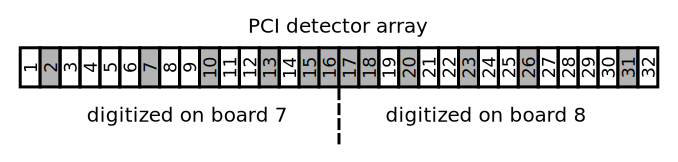
\includegraphics[width = \textwidth]{%
    Appendices/SpectralEstimation/figs/pci_detector_array.pdf}
  \caption[Schematic of PCI detector array]{%
    Schematic of PCI detector array.
    Only the gray channels are digitized.
  }
  \label{fig:SpectralEstimation:pci_detector_array}
\end{figure}

The PCI detector consists of $32$ elements arranged in a linear array.
However, due to digitization constraints,
only a subset of the signals from the linear array are digitized.
Further, to achieve reasonable mid-$k$ and high-$k$ response,
this subset of channels is non-uniformly spaced, as indicated in
Figure~\ref{fig:SpectralEstimation:pci_detector_array}.
This immediately precludes direct application
of the fast Fourier transform (FFT) in the spatial dimension, and
more elaborate schemes must be utilized
to quantify the spatial spectrum.
Below, Section~\ref{app:SpectralEstimation:2d_spectra:trigger_offset}
describes the estimation and compensation
of the trigger offset between the two PCI digitizer boards.
Then, Section~\ref{app:SpectralEstimation:2d_spectra:correlation_function}
discusses estimation of the two-dimensional autocorrelation function,
which can be computed even when channels are non-uniformly spaced.
Finally, Section~\ref{app:SpectralEstimation:2d_spectra:2d_spectra}
discusses calculation of the two-dimensional autospectral density
from the two-dimensional autocorrelation function.


\subsection{Estimation \& compensation of trigger offset}
\label{app:SpectralEstimation:2d_spectra:trigger_offset}
Prior to performing any spectral computations,
the trigger offset between
digitizer board $7$ and digitizer board $8$
must be estimated and compensated.
The general theory is discussed in
Appendix~\ref{app:DigitizerSynchronization}.
The trigger offset is estimated by defining
\begin{align}
  \Delta \alpha(f)
  &=
  \frac{\alpha_{15,16}(f) + \alpha_{17,18}(f)}{2}
  \\
  \Delta \alpha_{\meas}(f)
  &=
  \alpha_{16,17}(f),
\end{align}
and applying
(\ref{eq:DigitizerSynchronization:trigger_offset_estimate_apriori_phase});
here $\alpha_{i,j}(f)$ is the cross phase
between channels $i$ and $j$
during a stationary portion of the discharge.
To minimize random error,
at least $1000$ realizations are averaged over, and
only frequencies with sufficiently high coherence
(e.g.\ $\gamma^2_{i,j} \geq 0.1$) are considered.
The offset is rarely larger than one or two timestamps, but
even such small offsets can significantly bias spectral estimates.
Then, using standard techniques~\cite[Sec.~4.5]{oppenheim},
the trigger offset can be compensated easily in post-processing,
even if the offset is a non-integer multiple of the sample spacing.


\subsection{Two-dimensional autocorrelation function}
\label{app:SpectralEstimation:2d_spectra:correlation_function}
The autocorrelation function $R_{xx}$ and
the autospectral density function $S_{xx}$
are Fourier transform pairs, i.e.\
\begin{align}
  S_{xx}(\xi, f)
  &=
  \mathcal{F}[R_{xx}(\delta, \tau)](\xi, f),
  \label{eq:SpectralEstimation:autospectral_density_from_autocorrelation}
  \\
  R_{xx}(\delta, \tau)
  &=
  \mathcal{F}^{-1}[S_{xx}(\xi, f)](\delta, \tau),
  \label{eq:SpectralEstimation:autocorrelation_from_autospectral_density}
\end{align}
where
$\mathcal{F}$ is the Fourier transform,
$\tau$ is the temporal lag,
$\delta$ is the spatial lag,
$f$ is the frequency, and
$\xi$ is the spatial frequency
(related to the wavenumber $k$ via $k = 2 \pi \xi$).
If the measurements are uniformly sampled in space and time,
it is most efficient to estimate
the two-dimensional autospectral density $S_{xx}$
using the FFT methods described in
Section~\ref{app:SpectralEstimation:NonParametric} and
then apply the inverse Fourier transform
as in (\ref{eq:SpectralEstimation:autocorrelation_from_autospectral_density})
to compute the two-dimensional autocorrelation function $R_{xx}$.
However, if the measurements are \emph{not} uniformly spaced,
the two dimensional autocorrelation function
can still be estimated via the definition
\begin{equation}
  R_{xx}(\delta, \tau)
  =
  E[x_k(z, t) \cdot x_k(z + \delta, t + \tau)],
  \label{eq:SpectralEstimation:autocorrelation_definition}
\end{equation}
where $E[\cdot]$ is the expectation-value operator and
$x_k$ is the $k$\ts{th} realization
of the real-valued random process $\{x_k(z, t)\}$.
If needed, the autocorrelation can be interpolated onto a uniform grid, and
then the autospectral density $S_{xx}$ can be computed
by applying the Fourier transform,
as in (\ref{eq:SpectralEstimation:autospectral_density_from_autocorrelation}).

When temporal sampling is uniform but spatial sampling is nonuniform,
as in the PCI,
it is often convenient to define a
``hybrid'' two-dimensional autocorrelation function $\tilde{R}_{xx}$
\begin{align}
  \tilde{R}_{xx}(\delta, f)
  &=
  \mathcal{F}^{-1}[S_{xx}(\xi, f)](\delta)
  \notag \\
  &=
  \int_{-\infty}^{\infty}
  d\xi e^{i 2 \pi \xi \delta}
  S_{xx}(\xi, f)
  \notag \\
  &=
  S_{xx}(\delta, f),
\end{align}
where $S_{xx}(\delta, f) = S_{x_i, x_j}(f)$
is the cross-spectral density function
between $x_i(t) = x(z, t)$ and $x_j(t) = x(z + \delta, t)$.
Note that $S_{x_i, x_j}(f)$ can be efficiently computed
via the FFT methods described in
Section~\ref{app:SpectralEstimation:NonParametric}
such that the ``hybrid'' autocorrelation function can be estimated as
an ensemble average over all of the unique correlation pairs
separated by $\delta$
\begin{equation}
  \tilde{R}_{xx}(\delta, f)
  =
  \frac{%
    \sum\limits_{i - j = \delta} S_{x_i, x_j}(f)
  }{%
    \sum\limits_{i - j = \delta} 1
  };
  \label{eq:SpectralEstimation:hybrid_autocorrelation_estimate}
\end{equation}
if there are no correlation pairs separated by $\delta$,
then $\tilde{R}_{xx}$ is undefined for this separation.
If the variances of $x_i$ and $x_j$ are artificially biased
e.g.\ due to the finite PCI beam width,
the variances should be equalized prior to estimating $\tilde{R}_{xx}$ with
(\ref{eq:SpectralEstimation:hybrid_autocorrelation_estimate}).
As discussed in Section~\ref{app:SpectralEstimation:2d_spectra:2d_spectra},
the autospectral density can be computed
from this $\tilde{R}_{xx}$ estimate.

\begin{figure}
  \centering
  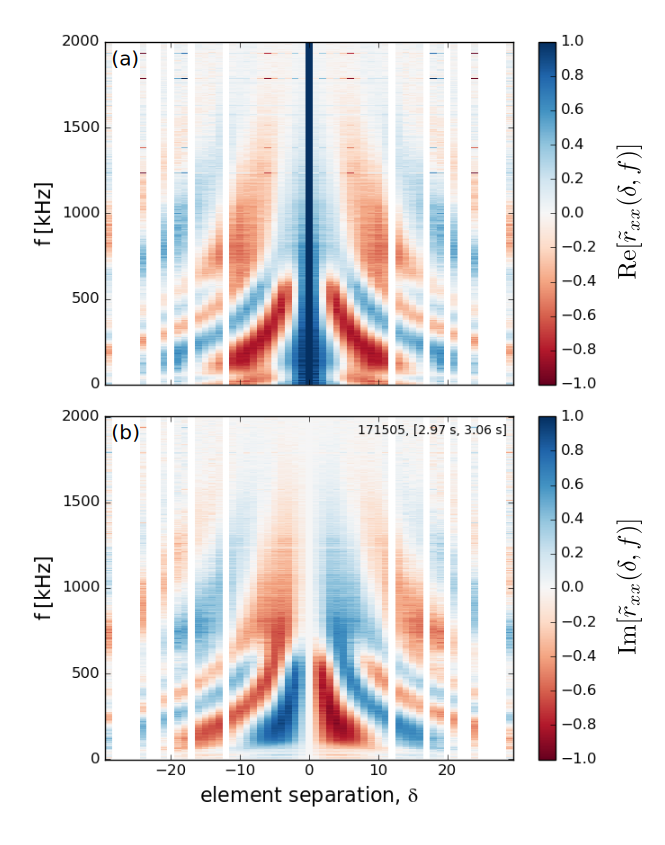
\includegraphics[width = 0.75 \textwidth]{%
    Appendices/SpectralEstimation/figs/corr_example.png}
  \caption[Normalized, $2$d, hybrid autocorrelation function]{%
    Example of the (a) real and (b) imaginary components
    of the PCI-measured normalized, two-dimensional, hybrid
    autocorrelation function $\tilde{r}_{xx}(\delta, f)$.
    Note that $\delta = 0$ corresponds to the same detector element,
    $\delta = 1$ corresponds to adjacent detector elements, etc.
    The vertical white striations correspond to
    non-existing element separations
    (as established by the digitization layout shown in
    Figure~\ref{fig:SpectralEstimation:pci_detector_array})
    for which $\tilde{r}_{xx}(\delta, f)$ is not defined.
    To proceed with the autospectral density estimation
    in Section~\ref{app:SpectralEstimation:2d_spectra:2d_spectra},
    the computation must either be restricted
    to the central, continuous domain, or
    the autocorrelation function must be interpolated;
    linear interpolation was found to be sufficient in this work.
  }
  \label{fig:SpectralEstimation:corr_example}
\end{figure}

Before proceeding, however, it is instructive
to consider a few properties of $\tilde{R}_{xx}$.
In general, $\tilde{R}_{xx}$ is complex-valued.
For real-valued $x$, however,
$\tilde{R}_{xx}$ is Hermitian,
i.e.\ $\tilde{R}_{xx}(-\delta, -f) = [\tilde{R}_{xx}(\delta, f)]^*$,
where $z^*$ indicates the complex conjugate of $z$.
At any given frequency $f$,
$|\tilde{R}_{xx}(\delta, f)|$ attains a maximum at $\delta = 0$.
The variance of signal $x(z, t)$ is related to $\tilde{R}_{xx}$ via
\begin{equation}
  \text{var}(x)
  =
  \int \tilde{R}_{xx}(0, f) df.
  \label{eq:SpectralEstimation:variance_relation_to_autocorrelation}
\end{equation}
Because $|\tilde{R}_{xx}|$ can vary by several orders of magnitude
across the full temporal bandwidth of signal $x(z, t)$,
visualizing the spatiotemporal structure of $\tilde{R}_{xx}$
can be aided by defining the normalized autocorrelation function
\begin{equation}
  \tilde{r}_{xx}(\delta, f)
  =
  \frac{\tilde{R}_{xx}(\delta, f)}{\tilde{R}_{xx}(0, f)}.
\end{equation}
An example of the PCI-measured $\tilde{r}_{xx}(\delta, f)$ is shown in
Figure~\ref{fig:SpectralEstimation:corr_example}.


\subsection{Two-dimensional autospectral density}
\label{app:SpectralEstimation:2d_spectra:2d_spectra}
The two-dimensional autospectral density function
$S_{xx}(k, f)$ can be computed from
the hybrid two-dimensional autocorrelation function
$\tilde{R}_{xx}(\delta, f)$.
Below and throughout this work,
if $\tilde{R}_{xx}(\delta, f)$ is not defined for a given $\delta$,
it is linearly interpolated across the gap.
Investigation of more sophisticated interpolation algorithms
is relegated to future work.

As suggested by
(\ref{eq:SpectralEstimation:autospectral_density_from_autocorrelation}),
computing the spatial Fourier transform of $\tilde{R}_{xx}(\delta, f)$
produces an estimate of the autospectral density $S_{xx}(k, f)$.
Explicitly,
\begin{align}
  S_{xx}(k, f)
  &=
  \mathcal{F} \left[ \tilde{R}_{xx}(\delta, f) \right](k)
  \notag \\
  &=
  \int_{-\infty}^{\infty}
  \tilde{R}_{xx}(\delta, f)
  e^{-i k \delta} d\delta
  \notag \\
  &\approx
  \int_{-\Delta / 2}^{\Delta / 2}
  \tilde{R}_{xx}(\delta, f)
  e^{-i k \delta} d\delta,
  \label{eq:SpectralEstimation:autospectral_density_from_autocorrelation_explicit}
\end{align}
where $\Delta = 2 \cdot \text{max}(|\delta|)$
is the full span of spatial lags.
Of course, for efficiency, the Fourier transform
should be computed via the FFT.
Further, to minimized sidelobe leakage,
$\tilde{R}_{xx}(\delta, f)$ should be windowed in $\delta$
prior to computing the Fourier transform;
here, only the Hanning window is considered.
Using the $\tilde{R}_{xx}(\delta, f)$ corresponding to
Figure~\ref{fig:SpectralEstimation:corr_example},
the resulting Fourier-in-space
autospectral density estimate is shown in
Figure~\ref{fig:SpectralEstimation:Skf_example}(a).
Clearly, the wavenumber resolution of the Fourier estimate
is severely limited by the sparse spatial sampling.

\begin{figure}
  \centering
  \includegraphics[width = 0.75 \textwidth]{%
    Appendices/SpectralEstimation/figs/Skf_example.png}
  \caption[$2$d autospectral density estimates]{%
    Two-dimensional autospectral density estimates $S_{xx}(k, f)$.
    Here, (a) estimates the spatial spectrum
    using conventional Fourier methods while
    (b) estimates the spatial spectrum
    using a $p = 4$ Burg AR evaluated
    on a uniformly spaced, $1000$-element wavenumber grid.
    It is important to note that
    the autospectral density estimates in both (a) and (b)
    correspond to the \emph{same} raw data and
    the \emph{same} autocorrelation function $\tilde{R}_{xx}(\delta, f)$
    from Figure~\ref{fig:SpectralEstimation:corr_example}.
    However, the Burg AR produces substantially improved
    wavenumber resolution.
  }
  \label{fig:SpectralEstimation:Skf_example}
\end{figure}

The parametric spectral-estimation techniques discussed in
Section~\ref{app:SpectralEstimation:Parametric}
present an alternative method for computing $S_{xx}(k, f)$.
For each frequency $f$ in $\tilde{R}_{xx}(\delta, f)$,
a $p$-order Burg AR can be performed in $\delta$
to estimate the autospectral density
of the \emph{autocorrelation function} $S_{\tilde{R}\tilde{R}}(k, f)$.
Now, from the non-parametric methods discussed in
Section~\ref{app:SpectralEstimation:NonParametric},
the autospectral density of $\tilde{R}_{xx}$ is defined as
\begin{equation}
  S_{\tilde{R}\tilde{R}}(k, f)
  =
  \lim_{\Delta \rightarrow \infty}
  \frac{1}{\Delta}
  E\left[%
    \left|
      \int_{-\Delta / 2}^{\Delta / 2}
      \tilde{R}_{xx}(\delta, f)
      e^{-i k \delta} d\delta
    \right|^2
  \right]
\end{equation}
such that
\begin{equation}
  \int_{-\Delta / 2}^{\Delta / 2}
  \tilde{R}_{xx}(\delta, f)
  e^{-i k \delta} d\delta
  \approx
  \pm \left[ \Delta \cdot S_{\tilde{R}\tilde{R}}(k, f) \right]^{1 / 2},
  \label{eq:SpectralEstimation:Fourier_transform_of_autocorrelation}
\end{equation}
which is real-valued because $S_{\tilde{R}\tilde{R}}$ and $\Delta$
are real-valued.
Substituting (\ref{eq:SpectralEstimation:Fourier_transform_of_autocorrelation})
into (\ref{eq:SpectralEstimation:autospectral_density_from_autocorrelation_explicit})
yields
\begin{equation}
  S_{xx}(k, f)
  \approx
  \left[
    \Delta
    \cdot
    S_{\tilde{R}\tilde{R}}(k, f)
  \right]^{1 / 2},
  \label{eq:SpectralEstimation:autospectral_density_Burg}
\end{equation}
where the positive root has been selected
because $S_{xx}(k, f)$ is positive semidefinite by definition.
Power conservation is ensured by normalizing
the spectral estimate to the signal variance, i.e.\
\begin{equation}
  \int S_{xx}(k, f) dk df
  =
  \text{var}(x),
\end{equation}
where $\text{var}(x)$ is related to $R_{xx}(\delta, f)$ via
(\ref{eq:SpectralEstimation:variance_relation_to_autocorrelation}).
Because the all-pole feature of an AR model
is capable of fitting very sharp spectral features
and the resulting spectral estimate can be evaluated
with an arbitrary resolution,
the wavenumber resolution of the Burg AR estimate
may be substantially better than that of the corresponding Fourier estimate,
as shown in Figure~\ref{fig:SpectralEstimation:Skf_example}(b).


\bibliographystyle{plainurl}
\bibliography{references}
%
\newcommand{\nom}{\text{nom}}
\newcommand{\trig}{\text{trig}}
\newcommand{\meas}{\text{meas}}


\chapter{Synchronization of digital records}
\label{app:DigitizerSynchronization}
\ldots
Efficient conversion of an analog signal to a digital record requires
quantization of the signal magnitude and
temporal sampling of these quantized magnitudes~\cite{bennett_bstj48}.


\section{Timebase of single digital record}
\label{app:DigitizerSynchronization:timebase_single_record}
Typically, temporal sampling of signal $x_j(t)$ occurs
at a fixed sampling rate $F_j$ such that
successive points in the digital record
are separated in time by $1 / F_j$.
Digitization begins at the ``trigger time'' $t_j[0]$ such that
the time corresponding to the $m\ts{th}$ digitized point is
\begin{equation}
  t_j[m] = t_j[0] + \frac{m}{F_j}.
  \label{eq:DigitizerSynchronization:timebase_generic}
\end{equation}
Ideally, the \emph{realized} sampling rate $F_j$ and trigger time $t_j[0]$
are equal to their \emph{nominal} values
$F_j^{\nom}$ and $t_j^{\nom}[0]$, respectively.
However, short-term jitter, long-term drifts, and constant offsets
often plague real-world digitization such that
$F_j \neq F_j^{\nom}$, $t_j[0] \neq t_j^{\nom}[0]$, and
\begin{equation}
  t_j[m] \neq t_j^{\nom}[0] + \frac{m}{F_j^{\nom}};
\end{equation}
that is, the actual time base of the digital record
does \emph{not} equal the nominal timebase.
In a properly operating digitizer,
these discrepancies are typically small, and
an autospectral-density estimate (for example)
of $x_j(t)$ from its digital record
will be negligibly compromised.
When estimating the \emph{phasing}
between $x_j(t)$ and $x_{k}(t)$ for $j \neq k$, however,
identifying and correcting such timebase discrepancies
becomes paramount in importance.


\section{Which digital records can be synchronized?}
\label{app:DigitizerSynchronization:digitization_schemes}
The digitization scheme determines
whether or not digital records
$\{x_j[m]\}$ and $\{x_k[m]\}$
can be synchronized.
The cleanest, simplest, and most problem-free scheme
is to digitize $x_j(t)$ and $x_k(t)$ on the \emph{same} system
such that the actual sample rates and trigger times
of both digital records are identical
(i.e.\ $F_j = F_k$ and $t_j[0] = t_k[0]$, respectively).
However, such a scheme is not always feasible.
Further, note that multiple digitizer boards
operating in a master-slave configuration
can still suffer from trigger-time offsets,
despite nominally being part of the same digitization system.
The next-best scheme is to use phase-locked digitizers
such that $F_j / F_k = F_j^{\nom} / F_k^{\nom}$,
regardless of any short-term jitter or long-term drift
in the digitizer clocks.
In general, phase-locked digitizers
still suffer from trigger offsets, which result
from the digitizers having different actual trigger times
(i.e.\ $t_j[0] \neq t_k[0]$) and
from each digitizer triggering at
an actual time that differs from its nominal trigger time
(e.g.\ $t_j[0] \neq t_j^{\nom}[0]$).
As shown in
Section~\ref{app:DigitizerSynchronization:phase_locked_synchronization},
it \emph{is} possible to synchronize records
from phase-locked digitizers.
Finally, the least-desirable scheme
is to use free-running digitizers
such that $F_j / F_k \neq F_j^{\nom} / F_k^{\nom}$;
it may be impossible to synchronize records
from free-running digitizers.


\section{Synchronization of phase-locked digital records}
\label{app:DigitizerSynchronization:phase_locked_synchronization}
\begin{itemize}
  \item Trigger offset
  \item Estimating trigger offset from constant-frequency mode
  \item Estimating trigger offset from mode with linearly ramped frequency
\end{itemize}


\subsection{The ``trigger offset''}
Phase-locked digitizers can still suffer from trigger offsets.
To see this, for digitizer $j$ define
$\delta t_j = t_j[0] - t_j^{\nom}[0]$
to be the difference between the actual and nominal trigger times,
$\delta F_j = F_j - F_j^{\nom}$
to be the difference between the actual and nominal sampling rates, and
$\bar{\delta F_j} = \delta F_j / F_j^{\nom}$
to be the relative difference between the actual and nominal sampling rates.
Then, to first order in $\bar{\delta F_j}$,
the actual digitization times $t_j[m]$
are related to the nominal digitization times $t_j^{\nom}[m]$ via
\begin{equation}
  t_j[m]
  \approx
  t_j^{\nom}[m]
  +
  \delta t_j
  -
  \frac{m \cdot \bar{\delta F_j}}{F_j^{\nom}}.
  \label{eq:DigitizerSynchronization:timebase_actual_vs_nominal}
\end{equation}
Thus, trigger-time discrepancy $\delta t_j$
produces a constant offset
between the actual and nominal timebases, while
sampling-rate discrepancy $\delta F_j$
produces a linear ramp
between the actual and nominal timebases.
Now, for phase-locked digitizers $j$ and $k$,
$\bar{\delta F_j} = \bar{\delta F_k}$
such that the corresponding ``trigger offset'' $\delta t_{\trig}$
between digital records $j$ and $k$ is
\begin{align}
  \delta t_{\trig}
  &=
  t_j[m] - t_k[m]
  \notag \\
  &=
  \left( \delta t_j - \delta t_k \right)
  +
  \bar{\delta F_j} \left( t_j^{\nom}[0] - t_k^{\nom}[0] \right).
  \label{eq:DigitizerSynchronization:trigger_offset}
\end{align}
Here, the first term on the right-hand side of
(\ref{eq:DigitizerSynchronization:trigger_offset})
corresponds to the difference between
trigger-time discrepancies of each digitizer, while
the second term on the right-hand side
corresponds to the relative sampling-rate discrepancy
weighted by the difference in nominal trigger times.
Note that (\ref{eq:DigitizerSynchronization:trigger_offset})
is valid even when $F_j^{\nom} \neq F_k^{\nom}$
(i.e.\ measurements made at different nominal sampling rates
can be upconverted or downconverted~\cite[Sec.~4.6]{oppenheim}
to the same nominal sampling rate, and
then (\ref{eq:DigitizerSynchronization:trigger_offset}) applies).


\subsection{Effect of the trigger offset}
The trigger offset (\ref{eq:DigitizerSynchronization:trigger_offset})
biases the phase of the digital record.
To see this, let $x_j(t)$ be a coherent mode
of angular frequency $\omega$ such that
the corresponding digital record is
\begin{align}
  x_j[m]
  &=
  x_j(t_j[m])
  \notag \\
  &=
  X_j(\omega) e^{-i \omega t_j[m]}
  \notag \\
  &=
  |X_j(\omega)| e^{i \{ \alpha_j(\omega) - \omega t_j[m]\}},
\end{align}
where $|X_j(\omega)|$ is the Fourier amplitude and
$\alpha_j(\omega)$ is the Fourier phase.
Then, the \emph{measured} phase difference $\Delta \alpha_{\meas}$
between digital records $\{x_j[m]\}$ and $\{x_k[m]\}$ is
\begin{align}
  \Delta \alpha_{\meas}
  &=
  \arg\left(
    x_k^*[m]
    \cdot
    x_j[m]
  \right)
  \notag \\
  &=
  \left[
    \alpha_j(\omega)
    -
    \alpha_k(\omega)
  \right]
  -
  \omega
  \left(
    t_j[m] - t_k[m]
  \right)
  \notag \\
  &=
  \Delta \alpha(\omega)
  -
  \left( \omega \cdot \delta t_{\trig} \right)
  \label{eq:DigitizerSynchronization:measured_phase_difference}
\end{align}
Thus, non-zero $\delta t_{\trig}$ biases
the measured phase difference $\Delta \alpha_{\meas}$
away from the true phase difference $\Delta \alpha$.
The above argument readily extends to broadband signals.


\subsection{Estimating the trigger offset}


\bibliographystyle{plainurl}
\bibliography{references}
%
% \chapter{External Clock}
\label{app:ExternalClock}

\begin{itemize}
  \item Cite D-tAcq documentation
\end{itemize}

% The frequency division is performed in `Dt216Init.fun` via the commands
% 
%     set.ext_clk DIx falling
%     setExternalClock DIx [div DOy]
% 
% The first command maps the external clock to digital input line
% `DIx` (x = {0, 1, 2, ..., 5)} and tells the digitizer what clock
% characteristic to sample on (here, the falling edge (as opposed to
% the rising edge)). The second command tells the digitizer to actually
% use the external clocking (as opposed to internal) by accepting a clock
% on digital input line `DIx` (x = {0, 1, 2, ..., 5}), optionally deriving
% a "local" clock by dividing by integer factor `div`, and also optionally
% outputting the derived local clock to digital output line
% `DOy` (y = {0, 1, 2, ...5}, with the constraint that x != y).
% 
% Note that the *minimum* value of `div` is 2. Note further that the commands
% *MUST* be issued in the above order to get correct clocking between the master
% and slave boards (described below); this is not well-documented in the
% user manuals, but it is absolutely essential.
% 
% I've hard-coded `div` = 4 to obtain a 4 MS/s sampling rate when using a
% 16 MHz external clock.
% 
% Master and slave board:
% -----------------------
% Previously, board 7 generated a local internal clock and distributed this
% to board 8 via the PXI backplane; for this reason, board 7's clock source
% (node name: `CLOCK_SRC`) was referred to as "MASTER" in the MDSplus tree.
% The trigger was accepted on board 8 and similarly distributed to board 7.
% 
% Attempting to "streamline" the logic, I've now designated board 8 as "MASTER".
% This means that board 8 accepts both the external clock and the trigger and
% distributes both to board 7 (the "slave"). This required making changes to
% the MDSplus tree.
% 
% Signal routing:
% ---------------
% Signal routing was altered in `Dt216Init.fun` and the MDSplus tree to realize
% the external clock and master-and-slave configuration discussed above. There
% are also some very slight tweaks to how the routing is done in
% `dt216__init.fun` and `dt216__store.fun` that are well-explained in the
% commentary surrounding the adjacent changes.
% 
% Note that the signal routing and the fact that the minimum value of `div`
% in the setExternalClock command (above) means that the maximum sample rate
% we can achieve with a 16 MHz external clock is 8 MS/s. (Sampling at the full
% 16 MS/s requires non-trivial changes to the routing).
% 
% Tests:
% ------
% As mentioned above, Mike's clock system has two spare outputs, each
% programmed to output a 16 MHz clock signal. The first output is used
% as our external clock input. The second output was connected to our
% divide-by-4 flip-flop circuit and digitized on ch. 8 and 16. Sampling
% at 16 MS/s (which required manually re-routing the clock signals etc),
% we expect a strong peak exactly at 4 MHz (corresponding to the fundamental
% frequency of the 4 MHz square wave). This is exactly what we see,
% as shown in the attached figure (`4MHz_signal_at_16MSPS.pdf`).
% 
% Also, when sampling at <= 8 MS/s (i.e. the normal signal routing I've
% implemented above), the phase difference between the signals is constant
% (i.e. no relative drift between boards, as is desired. Note that sampling
% at 8 MS/s allows us to just barely resolve the phase of the 4 MHz square wave
% at the digitizer Nyquist frequency). For some reason, however, when
% digitizing at 16 MS/s (with the altered routing), the phase of the signals
% digitized between the two boards is *not* constant, presumably resulting
% from some subtlety of the digitizer operation that I'm not quite grasping;
% however, by restricting our sample rates to <= 8 MS/s and using the usual
% routing, we shouldn't run into any problems :)

%
% \include{biblio}

\cleardoublepage\include{FrontBackmatter/Colophon}


\end{document}
